%\usepackage{wasysym}

\documentclass{book}
\usepackage{amsmath, amsfonts, amssymb}
\usepackage{Preamble}% options: nospade
\usepackage{paracol}


\DeclareMathOperator{\GL}{GL}
\DeclareMathOperator{\SL}{SL}
\DeclareMathOperator{\nul}{nul}
\DeclareMathOperator{\rank}{rank}
\DeclareMathOperator{\nullity}{nullity}
\DeclareMathOperator{\Span}{Span}
\DeclareMathOperator{\tr}{Tr}
\DeclareMathOperator{\sgn}{sgn}
\DeclareMathOperator{\Char}{Char}
\DeclareMathOperator{\Aut}{Aut}
\DeclareMathOperator{\Inn}{Inn}
\DeclareMathOperator{\End}{End}
\newcommand{\Ham}{\mathbb{H}}

%\usepackage{draftwatermark}
\usepackage{todonotes}
%todo list:  put tables into a box
%Preface
%Index
%nospade, search for [!HW!, label=$\spadesuit$ \arabic*., ref=\arabic*]
%%%%%%%%%%% Beginning of Document %%%%%%%%%%%

%\makeindex
%%https://raw.githubusercontent.com/emisseldine/MisselBooks/main/AbstractAlgebra/AbstractAlgebra.pdf
\begin{document}%\layout
\pagenumbering{gobble}

%\includepdf[fitpaper=true]{FrontMatter/cover2.pdf}%someone

%\begin{center}
%  \makebox[\textwidth]{\includegraphics[width=\paperwidth, height=0.75\paperheight]{FrontMatter/cover.pdf}}%Daven Triplett
%\end{center}

%Cover Page
\mbox{}\vfill
\resizebox{\linewidth}{!}{\sffamily\scshape Abstract}\vspace{5pt}
\resizebox{\linewidth}{!}{\sffamily\scshape Algebra}
\vfill\mbox{}\pagebreak\pagebreak

%%Dedication
%\mbox{}\vspace{25pt}
%\begin{center}
%\huge \scshape -- to Noelle\\
%\itshape ``Strive hard to do hard things''
%\end{center}\pagebreak

%Acknowledgements?

\copyleft{2025}
%\date{2025 Edition}
\date{\today}

\aboutAndrew

\title{Abstract Algebra}
\author{Andrew Misseldine}
\maketitle

\pdfbookmark{Table of Contents}{toc}
\tableofcontents

%\pagebreak
%\section*{Preface}
%This textbook is designed to guide you through the fundamental concepts of differential calculus, providing a comprehensive and accessible resource for your first collegiate calculus course.
%
%This book is heavily influenced by the clear and rigorous pedagogical style of Stewart Calculus, a classic in the field. While we've drawn inspiration from such excellent resources, great care has been taken to craft original examples and exercises that will challenge and solidify your understanding. Our goal is to make calculus engaging and intuitive, connecting abstract concepts to concrete applications.
%
%How This Book Is Organized
%This textbook is structured to align perfectly with a standard 4-credit, 15-week college semester. It's divided into 50 sections, with each section representing approximately one 50-minute lecture. This breakdown provides a natural pacing guide, ensuring that you can absorb the material effectively. Some topics span two sections, offering extra practice and reinforcement before you move on.
%
%The content is presented in a logical, developmental order, building concepts layer by layer. Each chapter corresponds to a unit exam, and while the primary arrangement is developmental, some topics have been strategically placed to balance the difficulty of these assessments. Within each section, you'll find clear definitions, illustrative examples, theorems with proofs, and a robust set of exercises to test your comprehension.
%
%To support your learning, final solutions are provided for all exercises, including complete proofs for problems requiring them. The only exceptions are the "Deeper Dive" questions, which are designed to offer more challenging problems for those seeking an extra intellectual push.
%
%Enhance Your Learning
%We believe in providing diverse tools to help you master calculus. Each section includes links to lecture videos created by the author, hosted on a dedicated YouTube channel. These videos offer an alternative explanation and visual demonstration of the concepts.
%
%Throughout the exercises and examples, you'll also find links to external websites like Desmos.com, offering interactive graphs or calculators. Many of these interactive tools were created by the author to enhance your understanding of specific concepts, while others are valuable resources from third parties. A comprehensive list of all external links (excluding the lecture videos) can be found in the back matter of this book. Additionally, useful formulas are conveniently located in the back of the book for quick reference.
%
%An Open Invitation
%This textbook was entirely written in LaTeX, a powerful typesetting system, allowing for precise mathematical formatting and high-quality presentation. All graphics were also created in LaTeX, with the exception of QR codes generated using Adobe.
%
%As an open-source textbook, we strongly believe in the power of collaboration and continuous improvement. We invite you to be a part of this journey! Your feedback is invaluable. If you find any typos, errors, areas that could be explained more clearly, or have suggestions for new examples and exercises, please don't hesitate to contribute. Information on how to provide feedback or contribute to this project can be found in the back matter. Together, we can make this an even better resource for future students.
%
%We hope this textbook empowers you to understand and appreciate the elegance and utility of calculus. Happy learning!
%%Preface/Introduction for Students:
%%
%%Welcome Message: A friendly introduction to the subject and the textbook.
%%Why this book? Briefly explain your philosophy or unique approach.
%%How to Use This Book: Guidance on effective study habits, how to navigate the book, and how to engage with exercises.
%%Prerequisites: Clearly state what mathematical background students should have.
%%Software/Tools Used (if applicable): Mention any specific software (e.g., graphing calculators, Desmos, Wolfram Alpha) or tools students might need.
%%Preface/Introduction for Instructors (Optional but recommended for OER):
%%
%%Pedagogical Approach: Elaborate on the teaching philosophy behind the book.
%%Customization Guide: Explain how instructors can adapt, remix, or contribute to the textbook. Provide guidance on accessing source files (e.g., LaTeX source, GitHub repository).
%%Suggested Course Pacing: Offer ideas for structuring a course using the textbook.
%%Instructor Resources: Mention if there are solutions manuals, problem banks, or other supplementary materials available.

\mainmatter

%%%%%%%%%%%% CHAPTER 1 %%%%%%%%%%%%%%%%%%%%
%%%%%%%%%%%%%%%%%%%%%%%%%%%%%%%%%%%%%%%%%%%%%%%%%%%%%%%%%%%%%%%%%%%%%%%%%%%%%%%%
\startHW
\chapterlabel{Abstract Prealgebra}{prealgebra}\pagebreak

%%%%%%%%%%%% Section 1.1 %%%%%%%%%%%%%%%%%%%%%%%%%%%%%%%%%%%%%%%%%%%%%%%%%%%%%%%%%%
%%%%%%%%%%%%%%%%%%%%%%%%%%%%%%%%%%%%%%%%%%%%%%%%%%%%%%%%%%%%%%%%%%%%%%%%%%%%
\begin{center} 
\emph{``What we call the beginning is often the end. And to make an end is to make a beginning. The end is where we start from.'' -- T. S. Eliot}
\end{center}


\begin{Videos}
\video{https://youtu.be/GLDPH62L72M}{Sets} &
\video{https://youtu.be/Khu_fHMbe6Y}{Subsets}  &
\video{https://youtu.be/HwqrbpJHdCY}{Algebra of Sets} &
\video{https://youtu.be/bD_y_aSlgGY}{Properties of Set Algebra}\\
\end{Videos}

\sectionlabel{Sets}{sets}

\begin{Def} A \textbf{set} is a well-defined collection of distinct objects. The objects of a set are called its \textbf{elements}. By \textbf{well-defined}, we mean that there is a rule that enables one to determine whether a given object is an element of the set or not. If a set has no elements, it is called the \textbf{empty set} and is denoted $\emptyset$ or $\{\}$.
\end{Def}\vs

A set is usually specified either by listing all of its elements inside a pair of braces or by stating the property that determines whether or not an object $x$ belongs to the set. We might write
\[X=\{x_1, x_2,\ldots,x_n\}\]
for a set containing elements $x_1, x_2,\ldots, x_n$ or 
\[X=\{x \mid x \text{ satisfies } \mathfrak{p}\}\]
if each $x$ in $X$ satisfies a certain property $\mathfrak{p}$.\\

Because elements in a set are distinct, we do not let repeats to occur in a set. In other words, the sets $\{1, 3, 2, 2\}$ and $\{1,3,2\}$ are the same, that is, \[\{1,3,2,2\} = \{1,3,2\}.\] Also, the order or arrangement of the elements in a set is irrelevant. So, \[\{1,2,3\} = \{1,3,2\} = \{3,2,1\}.\]

\begin{Def} When considering if an object is an element of a set or not, the symbol $\in$ means ``is an element of'' and $\notin$ means ``is not an element of.''
\end{Def}\vs

\begin{Exam} Let $A = \{1, 2, 3, 4\}$. To denote that $2$ is an element of the set $A$, we write $2\in A$. To denote that $5$ is not an element of $A$, we write $5\notin A$.
\end{Exam}\vs

Some famous sets include: 
\begin{eqnarray*}
\N &=& \{n\mid n \text{ is a natural number}\} = \{0, 1, 2, 3, 4, \ldots\};\\
\Z &=& \{n\mid n \text{ is an integer}\} = \{\ldots, -2, -1, 0, 1, 2, 3, 4, \ldots\};\\
\Q &=& \{r\mid r \text{ is a rational number}\} = \{p/q \mid p,q\in \Z \text{ where } q\neq 0\};\\
\R &=& \{x\mid x \text{ is a real number}\};\\
 \C &=& \{z\mid z \text{ is a complex number}\}.
\end{eqnarray*}

One can compare real numbers by determining whether one is bigger than the other or if they are the same. A similar comparison exists for sets.

 \begin{Def} Let $A$ and $B$ be two sets. If $A$ and $B$ have exactly the same elements as each other, then $A=B$.\\

 If every element of $A$ is an element of $B$, then $A$ is a \textbf{subset} of $B$ and we denote this as $A\subseteq B$. For example, \[\{1,2\} \subseteq \{1, 2, 3\}.\] Note that it is always true that $\emptyset \subseteq A$ for any set $A$. The reason this holds is that there exists no counterexamples, that is, there does not exist an element of $\emptyset$ which is not in $A$.\\

If $A\subseteq B$ and $A\neq B$, then $A\subset B$ and $A$ is a \textbf{proper subset} of $B$.\\

The \textbf{power set} of $A$, denoted $\mathcal{P}(A)$ is the set of all subsets of $A$. Hence, $X\in \mathcal{P}(A)$ if and only if $X\subseteq A$.
\end{Def}\vs

\begin{Exam} Consider the three sets $A = \text{the set of all even numbers}$, $B = \{2, 4, 6\}$, and $C = \{2,  3, 4, 6\}$.\\

Here, $B \subseteq A$ since every element of $B$ is also an even number, so is an element of $A$. Of course, $B\neq A$ since $8\in A$ but $8\notin B$. So, $B\subset A$.\\

It is also true that $B\subset C$. On the other hand, $C\not\subseteq A$ since $3\in C$ but $3\notin A$.
\end{Exam}\vs

\begin{Def} If $A$ and $B$ are sets, then the \textbf{intersection} of $A$ and $B$, denoted $A\cap B$, is the set consisting of elements that belong to both $A$ \emph{and} $B$. The \textbf{union} of $A$ and $B$, denoted $A\cup B$, is the set consisting of elements that belong to $A$ \emph{or} $B$ (or both).\\

For a list of sets $A_1, A_2,\ldots, A_n$, then 
\[\bigcap_{i=1}^n A_i = A_1\cap A_2 \cap \ldots \cap A_n \quad\text{and}\quad \bigcup_{i=1}^n A_i = A_1\cup A_2 \cup \ldots \cup A_n.\]\vs

Two sets are called \textbf{disjoint} if their intersection is empty.
\end{Def}\vs

\begin{Exam} Let $A = \{1, 3, 5, 8\}$, $B = \{3,5,7\}$, and $C = \{2,4,6,8\}$.
\begin{enumerate}
\item $A\cap B = \fbox{$\{3,5\}$}$\\
\item $A\cup B = \fbox{$\{1,3,5,7,8\}$}$\\
\item To calculate $B\cap (A\cup C)$, we first calculate $A\cup C$. 
\[A\cup C = \{1,2,3,4,5,6,8\}.\] Then \[B\cap(A\cup C) = \fbox{$\{3,5\}$}. \]
\end{enumerate}
\end{Exam}\vs

Usually, we will work with subsets of a bigger set, which we call the \textbf{universal set} $U$.

\begin{Def} If $A$ is a set, the \textbf{complement} of $A$, denoted $\overline{A}$, is the set of all elements in the universal set $U$ that are not in $A$. Other texts sometimes denote this as $A'$, $A^c$, or $\sim A$.
\end{Def}\vs

\begin{Exam} If the universal set $U = \{1,2,3,4,5,6,7,8,9\}$, $A = \{1,2,5,7,9\}$, and $B = \{1,2,4\}$, then \[\overline{A} = \fbox{$\{3,4,6,8\}$} \qquad\text{and}\qquad \overline{B} = \fbox{$\{3,5,6,7,8,9\}$}. \]
\end{Exam}\vs

\begin{Exam} Consider the sets $A =\{\text{red},\ \text{green},\ \text{blue}\}$ and $B=\{\text{red},\ \text{orange},\ \text{yellow},\ \text{green},\ \text{blue},\ \text{purple}\}$ inside the universal set of all colors. Then 
\[B\cap \overline{A} = \fbox{$\{\text{orange},\ \text{yellow},\ \text{purple}\}$}. \qedhere\]
\end{Exam}\vs

Note that in the previous example, the set $B\cap \overline{A}$ is the set of all elements of $B$ not contained in $A$. This is called the $\textbf{set difference}$ and is often denoted $B\setminus A$ or $B-A$. In this context, the set difference only depends on $B$ and $A$ and not on the universal set $U$ even though $A'$ depends on $U$.\\

Still considering the previous example, note that $A\setminus B = A\cap \overline{B} = \emptyset$ since every element of $A$ is contained in $B$. In fact, $A\subseteq B$. In general, if $A\subseteq B$ then $A\setminus B = \emptyset$.

\begin{Prop}\label{prop:setalgebra} For any set $A, B, C\subseteq U$,  
\begin{enumerate}[!THM!]
\item\label{item:setalgebra:idempotent} (Idempotency) $A\cup A = A$ and $A\cap A=A$;\\
\item\label{item:setalgebra:identity} (Identity) $A\cup \emptyset = A$ and $A\cap U = A$;\\
\item\label{item:setalgebra:absorb} (Absorption) $A\cup U = U$,  $A\cap \emptyset = \emptyset$, and $A\setminus \emptyset = A$;\\
\item\label{item:setalgebra:complement} (Complements) $A \cup \overline{A} = U$,  $A\cap \overline{A} = \emptyset$, and $A\setminus A = \emptyset$;\\
\item\label{item:setalgebra:commute} (Commutativity) $A\cup B = B\cup A$ and $A\cap B = B\cap A$;\\
\item\label{item:setalgebra:associate} (Associativity) $A\cup (B\cup C) = (A\cup B)\cup C$ and $A\cap (B\cap C) = (A\cap B)\cap C$;\\
\item\label{item:setalgebra:distribute} (Distributivity) $A\cup (B\cap C) = (A\cup B) \cap (A\cup C)$ and $A\cap (B\cup C) = (A\cap B) \cup (A\cap C)$;\\
\item\label{item:setalgebra:demorgan} (De Morgan's Laws) $\overline{A\cap B} = \overline{A}\cup \overline{B}$ and $\overline{A\cup B} = \overline{A} \cap \overline{B}$.
\end{enumerate}
\end{Prop}
\begin{pf}
Many of these identities are straight forward to prove and many will be proven in the homework. To illustrate the basic template for proving two sets are equal we prove the first distributive law $A\cup (B\cap C) = (A\cup B) \cap (A\cup C)$. To prove that two sets are equal, we will show that the two sets are subsets of each other.\\

We begin by showing that $A\cup (B\cap C) \subseteq (A\cup B) \cap (A\cup C)$. Let $x\in A\cup (B\cap C)$. So, $x\in A$ or $x\in B\cap C$. Suppose first that $x\in A$. Now, $A\subseteq A\cup B, A\cup C$. So, $x\in A\cup B, A\cup C$. Thus, $x\in (A\cup B)\cap (A\cup C)$. Next, suppose that $x\in B\cap C$. So, $x\in B$ and $x\in C$. Now, $B\subseteq A\cup B$ and $C\subseteq A\cup C$. Thus, $x\in (A\cup B)\cap (A\cup C)$. Either way, we get $A\cup (B\cap C) \subseteq (A\cup B) \cap (A\cup C)$.\\

Next, we show that $(A\cup B) \cap (A\cup C) \subseteq A\cup (B\cap C)$. Let $x\in (A\cup B)\cap (A\cup C)$. So, $x \in A\cup B$ and $x\in A\cup C$. If $x\in A$, then $x\in A\cup (B\cap C)$ and we're done. Suppose then that $x\notin A$. That implies that $x\in B$ and $x\in C$. Thus, $x\in B\cap C$. Therefore, $x\in A\cup (B\cap C)$, which implies that $(A\cup B) \cap (A\cup C) \subseteq A\cup (B\cap C)$. \\

Combining the two statements, this shows that $A\cup (B\cap C) = (A\cup B) \cap (A\cup C)$.
\end{pf}\vs

\vfill
\stepcounter{footnote}\footnotetext{See \href{http://abstract.ups.edu/aata/ssets-ection-sets-and-equivalence-relations.html}{\S 1.2 Sets and Equivalence Relations} in Judson's \href{https://judsonbooks.org/aata/}{Abstract Algebra: Theory and Applications} for additional reading.}
\pagebreak

\startExercises{sets}

For Exercises \ref{exer:setalgebra:start}--\ref{exer:setalgebra:stop}, suppose that 
\[A=\{n\mid n\in \N, n \text{ is even}\},\quad B = \{n\mid n\in \N, n \text{ is prime}\},\quad C =\{n\mid n\in \N, 5 \mid n\}.\] Describe the given set.
\begin{multicols}{4}
\begin{enumerate}[!HW!]
\item\label{exer:setalgebra:start} $A\cap B$
\item $B\cap C$
\item $A\cup B$
\item\label{exer:setalgebra:stop}  $A\cap (B\cup C)$\\
\end{enumerate}
\end{multicols}\vs

For Exercises \ref{exer:setproof:start}--\ref{exer:setproof:stop}, for any set $A,B,C\subseteq U$, prove the given set identity.\\ \textbf{\color{cyan} (Pick 2 from Exercises \ref{exer:setproof:start}-\ref{exer:setproof:pickstop}; Pick 2 from Exercises \ref{exer:setproof:pickstart}-\ref{exer:setproof:stop})}
\begin{enumerate}[!HW!]
\begin{multicols}{3}
\item \label{exer:setproof:start} \propref{prop:setalgebra} \ref{item:setalgebra:idempotent}
\item \propref{prop:setalgebra} \ref{item:setalgebra:identity}
\item \propref{prop:setalgebra} \ref{item:setalgebra:absorb}
\end{multicols}
\begin{multicols}{3}
\item \propref{prop:setalgebra} \ref{item:setalgebra:complement}
\item \propref{prop:setalgebra} \ref{item:setalgebra:commute}
\item \propref{prop:setalgebra} \ref{item:setalgebra:associate}
\end{multicols}
\begin{multicols}{3}
\item \propref{prop:setalgebra} \ref{item:setalgebra:distribute}
\item  \propref{prop:setalgebra} \ref{item:setalgebra:demorgan}
\item $A\subseteq B$ iff $A\cap B=A$
\end{multicols}
\begin{multicols}{2}
\item \label{exer:setproof:pickstop} $A\cup B = (A\cap B)\cup (A\setminus B)\cup (B\setminus A)$
\item \label{exer:setproof:pickstart} $(A\cap B)\setminus B = \emptyset$
\end{multicols}
\begin{multicols}{2}
\item $(A\cup B)\setminus B = A\setminus B$
\item $A\setminus (B\cup C) = (A\setminus B) \cap (A\setminus C)$
\end{multicols}
\begin{multicols}{2}
\item $A\cap (B\setminus C) = (A\cap B)\setminus (A\cap C)$
\item \label{exer:setproof:stop} $(A\setminus B)\cup (B\setminus A) = (A\cup B)\setminus (A\cap B)$
\end{multicols}
\end{enumerate}

\pagebreak


%%%%%%%%%%%% Section 1.2 %%%%%%%%%%%%%%%%%%%%%%%%%%%%%%%%%%%%%%%%%%%%%%%%%%%%%%%%%%
%%%%%%%%%%%%%%%%%%%%%%%%%%%%%%%%%%%%%%%%%%%%%%%%%%%%%%%%%%%%%%%%%%%%%%%%%%%%
\begin{center} 
\emph{``The function of education is to teach one to think intensively and to think critically. Intelligence plus character -- that is the goal of true education.'' -- Martin Luther King, Jr.}
\end{center}

\begin{Videos}
\video{https://youtu.be/JZB5_fKd2C8}{Cartesian Products} &
\video{https://youtu.be/8PX2Wi2apfI}{Function Composition}  &
\video{https://youtu.be/1gQfUT6NDbI}{Injective and\\ Surjective Functions} &
\video{https://youtu.be/_D48Iu6kJR8}{Properties of Functions}
\end{Videos}

\sectionlabel{Functions}{function}

\begin{Def} Given sets $A$ and $B$, we can define a new set $A\times B$, called the \textbf{Cartesian product} of $A$ and $B$, as a set of ordered pairs. That is,
\[A\times B=\{(a,b) \mid a\in A \text{ and } b\in B\}.\]\vs

We define the Cartesian product of $n$ sets to be
\[\prod_{i=1}^n A_i = A_1\times\ldots\times A_n = \{(a_1,\ldots,a_n) \mid a_i\in A_i \text{ for } i=1,\ldots,n\}.\]
If $A=A_1=A_2=\ldots=A_n$, we often write $A^n$ for $A\times\ldots\times A$ (where $A$ would be written $n$ times). For example, the set $\mathbb{R}^3$ consists of all of 3-tuples of real numbers.
\end{Def}\vs

\begin{Exam} If $A=\{x, y\}$, $B=\{1,2,3\}$, and $C=\emptyset$, then $A\times B$ is the set 
\[A\times B = \{(x,1), (x,2), (x,3), (y,1), (y,2), (y,3)\}\quad\text{and}\quad A\times C=\emptyset.\qedhere\]
\end{Exam}\vs

\begin{Def} A \textbf{relation} $R$  between the sets $A$ and $B$ is a subset of their Cartesian product, that is, $R\subseteq A\times B$. For elements $a\in A$ and $b\in B$, we say that $a$ is \textbf{related to} $b$ with respect to $R$, denoted $a\ R\ b$, if and only if $(a,b) \in R$. \\

We say that a relation $f\subseteq A\times B$ is a \textbf{function} or \textbf{mapping} from set $A$ to set $B$, denoted $f : A \to B$ or $A \xrightarrow{f} B$, if each element $a\in A$ occurs in exactly one ordered pair of the form $(a,b)$ in $f$, that is, each $a\in A$ is related to exactly one $b\in B$. This unique element $b$ is called the \textbf{image} of $a$ with respect to $f$, and this unique relationship is expressed as $f(a) = b$ or $f : a \mapsto b$. The set $A$ is called the \textbf{domain} of $f$, the set $B$ is called the \textbf{codomain} of $f$,  the set 
\[f(A) = \{f(a) \mid a\in A\}\] is called the \textbf{image} (or \textbf{range}) of $f$, and, any subset $X\subseteq B$, the set \[f^{-1}(X) = \{a\in A\mid f(a) \in X\}\] is called the \textbf{pre-image} of $X$ with respect to $f$. \\

Let $B^A$ denote the set of all functions of the form $f : A\to B$. This notation is used because if $|A| = a$ and $|B| = b$, then $|B^A| = b^a$, where $|S|$ denotes the cardinality of the set $S$.
\end{Def}\vs

\begin{Exam} In calculus, functions between real numbers are often defined using formulas such as $f(x) = x^3$ or $g(x) = e^x$. Such function expressions are to be understood as meaning the mapping $f :  x \mapsto f(x)$ is given by substitution, for example $f(2) = (2)^3 = 8$ and $g(0) = e^0 = 1$.\\

 In this context, the domain and codomain  is usually not stated, but the convention is to set them as the maximal subsets of $\R$ such that $f(x)\in \R$ for each $x\in \dom f$. For example, if $f_1(x) = \dfrac{1}{x}$ and $f_2(x) = \sqrt{x}$, then $f_1(0)$ and $f_2(-1)$ do not evaluate to be real numbers. Therefore, the convention is to restrict the sets so that 
\[f_1 : (\-\infty, 0)\cup (0,\infty) \to (\-\infty, 0)\cup (0,\infty)\quad\text{and}\quad f_2 : [0,\infty) \to [0,\infty). \] On the other hand, the functions above have the form
\[f : \R \to \R\qquad\text{and}\qquad g : \R\to (0,\infty). \qedhere\]
\end{Exam}\vs

\begin{Exam} Consider the relation $f : \Q \to \Z$ given by $f(p/q) = p$. We know that $\dfrac{1}{2} = \dfrac{2}{4}$, but is $f\left(\dfrac{1}{2}\right) = 1$ or $2$? This relation cannot be a mapping because it is not \emph{well-defined}. A relation is \textbf{well-defined} if each element in the domain is assigned to a unique element in the range. This is particularly a problem when ``mappings'' are defined on sets of equivalence classes\footnotemark\ according to representatives from the classes. If not carefully defined, such ``mappings'' might not be functions.
\end{Exam}\vs

\begin{Def} Given two functions $f : B\to C$ and $g : A\to B$\footnotemark\ the \textbf{composition} of $f$ and $g$, denoted $f\circ g : A\to C$,  is defined by \[(f\circ g)(x) = f(g(x)).\]
\end{Def}\vs

\begin{Exam} If $f(x) = x^3$ and $g(x) = e^x$, then  $(f\circ g)(x) = (e^x)^3 = e^{3x}$. \end{Exam}\vs

\begin{Def} Let $f : A \to B$ be a function. Let $a_1, a_2 \in A$. We say that $f$ is \textbf{injective} or \textbf{one-to-one} if $f(a_1) = f(a_2)$ implies that $a_1 = a_2$, or in other words,  for each $b\in f(A)$ there is a unique $a\in A$ such that $f(a) = b$.\\ 


We say that $f$ is \textbf{surjective} or \textbf{onto} if the image of $f$ equals the codomain of $f$ ($f(A) = B$), or in other words, for all $b\in B$ there exists an $a\in A$ such that $f(a) = b$.\\

If $f$ is both injective and surjective, then we say that $f$ is \textbf{bijective}.
\end{Def}\vs

\begin{Exam} If $f : \R \to \R$, $g: \R \to \R$, and $h : \R\to \R$ given by $f(x) = x^3$, $g(x) = e^x$, and $h(x) =x^2$, then $f$ is bijective, $g$ is injective but not surjective, and $h$ is neither injective nor surjective. On the other hand, the mapping $g_1 : \R \to (0,\infty)$ and $h_1 : \R \to [0,\infty)$ given by $g_1(x) = e^x$ and $h_2(x) = x^2$ are both surjective maps but only $g_1$ is injective. If we consider $h_2(x) : [0,\infty) \to [0, \infty)$ given by $h_2(x) = x^2$, then $h_2$ is bijective. For these reasons, the convention for defining functions in calculus is very imprecise for higher mathematics.
\end{Exam}\vs

\begin{Thm}\label{thm:functioncompose} Let $f: A\to B$, $g : B\to C$, and $h : C\to D$. Then
\begin{enumerate}[!THM!, start=1]
\item\label{item:functioncompose:a} The composition of mappings is associative, that is, $(h\circ g)\circ f = h\circ (g\circ f)$;\\
\item\label{item:functioncompose:b} If $f$ and $g$ are both surjective, then $g\circ f$ is surjective;\\
\item\label{item:functioncompose:c} If $f$ and $g$ are both injective, then $g\circ f$ is injective;\\
\item\label{item:functioncompose:d} If $f$ and $g$ are both bijective, then $g\circ f$ is bijective.
\end{enumerate}
\end{Thm}
\begin{pf}
Let $a\in A$. Then 
\[[(h\circ g)\circ f ](a) = (h\circ g)(f(a)) = h(g(f(a))) = h((g\circ f)(a)) = [h\circ (g\circ f)](a),\] which proves \ref{item:functioncompose:a}.\\

Let $c\in C$. Since $g$ is surjective, there exists some $b\in B$ such that $g(b) =c$. Likewise, since $f$ is surjective, there exists some $a\in A$ such that $f(a) = b$. Thus, 
\[(g\circ f)(a) = g(f(a)) = g(b) = c,\] which proves \ref{item:functioncompose:b}.\\

Part \ref{item:functioncompose:c} is left as an exercise to the student. Part \ref{item:functioncompose:d} follows immediately from \ref{item:functioncompose:b} and \ref{item:functioncompose:c}.
\end{pf}


\vfill
\footnotetext[1]{Equivalence relations will be reviewed in the \secref{equivalence}.}
\footnotetext{It is not necessary that the codomain of $g$ and domain of $f$ be equal. Instead function composition can be defined when the domain of $f$ is a subset of the codomain of $g$.}
\stepcounter{footnote}\footnotetext{See \href{http://abstract.ups.edu/aata/ssets-ection-sets-and-equivalence-relations.html}{\S 1.2 Sets and Equivalence Relations} in Judson's \href{https://judsonbooks.org/aata/}{Abstract Algebra: Theory and Applications} for additional reading.}
\pagebreak

\startExercises{function}

For Exercises \ref{exer:cartesianproduct:start}--\ref{exer:cartesianproduct:stop}, suppose that 
\[A=\{a,b,c\},\quad B = \{1,2,3\},\quad C =\{x\}, \quad D=\emptyset.\] List all of the elements in the given set. 
\begin{multicols}{4}
\begin{enumerate}[!HW!]
\item\label{exer:cartesianproduct:start} $A\times B$
\item $B\times A$
\item $A\times B\times C$
\item\label{exer:cartesianproduct:stop}  $A\times D$
\end{enumerate}
\end{multicols}\vs

For Exercises \ref{exer:welldefined:start}--\ref{exer:welldefined:stop}, determine if the given relation $f:\Q\to \Q$ is a function. Explain why or why not.
\begin{multicols}{4}
\begin{enumerate}[!HW!]
\item\label{exer:welldefined:start} $f\left(\dfrac{p}{q}\right) = \dfrac{p+1}{p-2}$
\item $f\left(\dfrac{p}{q}\right) = \dfrac{3p}{3q}$
\item $f\left(\dfrac{p}{q}\right) = \dfrac{p+q}{q^2}$
\item\label{exer:welldefined:stop}  $f\left(\dfrac{p}{q}\right) = \dfrac{3p^2}{7q^2}-\dfrac{p}{q}$
\end{enumerate}
\end{multicols}\vs

For Exercises \ref{exer:onetoone:start}--\ref{exer:onetoone:stop}, determine if the given function is injective or surjective. 
\begin{enumerate}[!HW!]
\begin{multicols}{2}
\item\label{exer:onetoone:start} $f:\R\to\R:f(x)=e^x$
\item $f:\Z\to\Z: f(n)=n^2+3$
\end{multicols}
\begin{multicols}{2}
\item $f:\R\to\R:f(x)=\sin x$
\item\label{exer:onetoone:stop}  $f:\R\to\R:f(x)=x^3-3x$
\end{multicols}
\end{enumerate}\vs

For Exercises \ref{exer:notonto:start}--\ref{exer:notonto:stop}, define a function $f:\N\to \N$ with the given properties. Explain why $f$ has the given properties.
\begin{enumerate}[!HW!]
\begin{multicols}{2}
\item\label{exer:notonto:start} Injective but not surjective
\item\label{exer:notonto:stop} Surjective but not injective
\end{multicols}
\end{enumerate}\vs

For Exercises \ref{exer:functionproof:start}--\ref{exer:functionproof:stop}, let $f:A\to B$ and $g:B\to C$ be functions. Prove the given statement.
\begin{enumerate}[!HW!]
\item \label{exer:functionproof:start} If $f$ and $g$ are both injective functions, then $g\circ f$ is injective.
\item If $g\circ f$ is surjective, then $g$ is surjective.
\item If $g\circ f$ is injective, then $f$ is injective. 
\item If $g\circ f$ is injective and $f$ is surjective, then $g$ is injective.
\item \label{exer:functionproof:stop}If $g\circ f$ is surjective and $g$ is injective, then $f$ is surjective.
\end{enumerate}

\pagebreak

%%%%%%%%%%%% Section 1.3 %%%%%%%%%%%%%%%%%%%%%%%%%%%%%%%%%%%%%%%%%%%%%%%%%%%%%%%%%%
%%%%%%%%%%%%%%%%%%%%%%%%%%%%%%%%%%%%%%%%%%%%%%%%%%%%%%%%%%%%%%%%%%%%%%%%%%%%
\begin{center} 
\emph{``My happiness grows in direct proportion to my acceptance, and in inverse proportion to my expectations.'' -- Michael J. Fox}
\end{center}

\begin{Videos}
\video{https://youtu.be/r-IPV76_WkQ}{Invertible Functions} &
\video{https://youtu.be/_IZu1hYQFbU}{Invertible Functions are Bijective}  &
\video{https://youtu.be/ZOQb_50uN4c}{Permutations} 
\end{Videos}

\sectionlabel{Inverse Functions and Permutations}{inverse}

\begin{Exam} Consider the mapping $f : A\to A$, with $A\neq \emptyset$ defined by the rule $f(a) = a$ for all $a\in A$. This mapping is known as the \textbf{identity function}, is denoted $id_A$, and is always bijective.\end{Exam}\vs

\begin{Def} Let $f : A\to B$ be a function. We say that $f$ is \textbf{invertible} if there exists a function $f^{-1} : B \to A$, called the \textbf{inverse} of $f$, such that
\[f^{-1} \circ f = id_A \qquad\text{and}\qquad f\circ f^{-1} = id_B.\]
\end{Def}\vs

When an inverse exists, it is unique. We will see that this is a property true for all groups.

\begin{Exam} The functions $f(x) = x^3$ and $g(x) = e^x$ are invertible, real-valued functions since $f^{-1}(x) = \sqrt[3]{x}$ and $g^{-1}(x) = \ln x$. Note that $f^{-1} : \R \to \R$ and $g^{-1} : (0,\infty) \to \R$.\\

On the other hand, the function $h_1 : \R \to [0,\infty)$ given by $h_1(x) = x^2$ is NOT invertible. It is tempting to believe that $h_1^{-1}(x) = \sqrt{x}$, but this is where the domain/codomain conventions of calculus can be ambiguous. Note that although $\sqrt{x}^2 = x$ for all $x  \ge 0$, we have $\sqrt{x^2} = |x|$, which does not equal $x$ for $x < 0$. On the other hand, the mapping $h_2 : [0,\infty) \to [0,\infty)$ given by $h_2(x) = x^2$ is invertible with $h_2^{-1}(x) = \sqrt{x}$. It is important to recognize that as functions $h_1\neq h_2$  even though they are defined by the same mathematical formula. 
\end{Exam}\vs

The reason that $h_1$ is not invertible in the previous example essentially comes down to the fact that $h_1$ is not bijective.

\begin{Thm} A mapping is invertible if and only if it is both one-to-one and onto.\end{Thm}
\begin{pf}
Let $f : A\to B$. If $f$ is bijective, then for each $b\in B$ there is a unique $a\in A$ such that $f(a) = b$. Define a mapping $g : B\to A$ such that $g(b) = a$ exactly when $f(a) = b$. By the unique statement mentioned before, $g$ is well-defined. Next, note that $f\circ g = id_B$ and $g\circ f = id_A$. Therefore, $f$ is invertible.\\

If $f$ is invertible, then $f\circ f^{-1} = id_B$, which is a surjective map. By exercise 1.3.22 (b), $f$ is surjective. Likewise, $f^{-1}\circ f = id_A$, which is an injective map. By exercise 1.3.22 (c), $f$ is injective. Therefore, $f$ is bijective.
\end{pf}\vs

\begin{Exam} Let $A$ be an $m\times n$ matrix. Then this matrix naturally produces a linear transformation $T : \R^n\to \R^m$ using the rule
\[T(\bb x) = A\bb x.\] As was learned in Linear Algebra class, an $n\times n$ matrix $A$ is invertible, it has an inverse $A^{-1}$ if and only if $A$ is nonsingular, that is, $A\bb x = \bb b$ has a unique solution. Notice that this statement is a special case of the previous theorem. We note that $A$ being nonsingular is the same thing as $T$ being bijective. Note that $A\bb x = \bb b$ having a solution means that $\bb b$ is the image of some vector $\bb x$ via $T$, that is, $T(\bb x) = \bb b$. This is surjectivity. Likewise, since $A\bb x = \bb b$ has a unique solution means there is exactly one vector $\bb x$ such that $A\bb x = \bb b$. Thus, there is only one vector $\bb x$ such that $T(\bb x) = \bb b$. This is injectivity.
\end{Exam}\vs

\begin{Def} For any set $X$, a bijective mapping $\pi : X \to X$ is called a \textbf{permutation} of $X$. The set of permutations on $X$ is denoted $S_X$. When the set has the form $X = \{1, 2, \ldots, n\}\subseteq \N$, we denote $S_X$ as $S_n$.
\end{Def}\vs

When working with permutations on a finite set $X$, it can be convenient to use a two--row tableaux to express the permutation, where the first row is an arrangement of the elements of $X$ and the second row is the images of the first row with respect to $\pi$. Thus, the second row will be a rearrangement of  the elements of $X$, which is why these maps are called permutations. For example, the permutation $\pi : X\to X$ where $X = \{1,\ldots, n\}$ might have the form
\[\pi = \left(\begin{array}{ccccc} 1 & 2 & \cdots & n\\ \pi(1) & \pi(2) & \cdots & \pi(n)\end{array}\right).\]\vs 

\begin{Thm} Let $X$ be a finite, nonempty set. Then $|S_X| = |X|!$.\end{Thm}
\begin{pf} Without the loss of generality, we may assume that $X = \{1,\ldots, n\}$, where $n= |X|$. Let $\pi : X\to X$ be a permutation. Then there are $n$ choices for the assignment $\pi(1)$ since $1$ can be mapped to any element of $X$. Likewise, there are $n-1$ choices for the assignment $\pi(2)$ since $2$ can be mapped to any element of $X$ other than $\pi(1)$. This is to guarantee that $\pi$ is injective. Likewise, there are $n-3$ choices for $\pi(3)$, since it can be any element of $X$ except $\pi(1)$ and $\pi(2)$. Continuing in this pattern, there will always be $n-k+1$ choices for $\pi(k)$. Finally, the product of these choices will give us the correct number of permutation which is $n\cdot (n-1) \cdot (n-2) \cdots 1=n!$.
\end{pf}\vs

\begin{Exam} Suppose that $X = \{1, 2, 3\}$. Define a map $\pi  : X \to X$ by
\[\pi(1) = 2,\quad \pi(2) = 1,\quad \pi(3) = 3\]
This is a bijective map and hence a permutation. In particular, 
\[\pi  =  \left(\begin{array}{ccc} 1 & 2 & 3 \\ \pi(1) & \pi(2) & \pi(3)\end{array}\right) = \left(\begin{array}{ccc} 1 & 2 & 3 \\ 2 & 1 & 3\end{array}\right).\]

There are five other elements of $S_3$:
\[id_X = \left(\begin{array}{ccc} 1 & 2 & 3 \\ 1 & 2 & 3\end{array}\right),\quad \left(\begin{array}{ccc} 1 & 2 & 3 \\ 1 & 3 & 2\end{array}\right), \left(\begin{array}{ccc} 1 & 2 & 3 \\ 2 & 3 & 1\end{array}\right),\]
\[\pi = \left(\begin{array}{ccc} 1 & 2 & 3 \\ 2 & 1 & 3\end{array}\right),\quad \left(\begin{array}{ccc} 1 & 2 & 3 \\ 3 & 2 & 1\end{array}\right), \quad \left(\begin{array}{ccc} 1 & 2 & 3 \\ 3 & 1 & 2\end{array}\right)\]

It is always possible to compose two permutations since they have the same domains as codomains, and this composite will itself be a permutation. A three-row tableaux can be used to compute their composite. The right two rows will be the same as the permutation on the right, but the third row will be the image of this second row by the permutation on the left. For example, \[\left(\begin{array}{ccc} 1 & 2 & 3 \\ 3 & 2 & 1\end{array}\right)\circ \left(\begin{array}{ccc} 1 & 2 & 3 \\ 2 & 1 & 3\end{array}\right) = \left(\begin{array}{ccc} 1 & 2 & 3 \\ 2 & 1 & 3 \\ 2 & 3 & 1\end{array}\right) = \left(\begin{array}{ccc} 1 & 2 & 3 \\ 2 & 3 & 1\end{array}\right).\]




Permutations always have inverses since they are bijective. They can be easily construct by reflecting the above permutation tableaux (and reordering the elements, if necessary). For example, $\pi^{-1} : S \to S$ is given as 
\[\pi^{-1} =  \left(\begin{array}{ccc} \pi(1) & \pi(2) & \pi(3)\\ 1 & 2 & 3 \end{array}\right) = \left(\begin{array}{ccc} 2 & 1 & 3\\ 1 & 2 & 3  \end{array}\right) = \left(\begin{array}{ccc} 1 & 2 & 3\\ 2 & 1 & 3  \end{array}\right) = \pi.\] Interesting enough, this permutation is equal to its own inverse, although this is not always the case.
\end{Exam}\vs

\vfill

\stepcounter{footnote}\footnotetext{See \href{http://abstract.ups.edu/aata/ssets-ection-sets-and-equivalence-relations.html}{\S 1.2 Sets and Equivalence Relations} in Judson's \href{https://judsonbooks.org/aata/}{Abstract Algebra: Theory and Applications} for additional reading.}
\pagebreak

\startExercises{inverse}

For Exercises \ref{exer:inversefunction:start}--\ref{exer:inversefunction:stop}, let $f:X\to Y$ be a function with $A_1,A_2\subseteq X$ and $B_1,B_2\subseteq Y$. Note we are not assuming that $f$ is invertibilty, but the pre-image $f^{-1}(B_1)=\{x \in X\mid f(x)\in B_1\}$ is well-defined regardless. Prove the given identity.
\begin{enumerate}[!HW!]
\begin{multicols}{2}
\item\label{exer:inversefunction:start} $f(A_1\cup A_2)=f(A_1)\cup f(A_2)$
\item $f(A_1\cap A_2)\subseteq f(A_1)\cap f(A_2)$;\\ Given an example where equality fails.
\end{multicols}
\begin{multicols}{2}
\item $f^{-1}(B_1\cup B_2)=f^{-1}(B_1)\cup f^{-1}(B_2)$
\item $f^{-1}(B_1\cap B_2)=f^{-1}(B_1)\cap f^{-1}(B_2)$
\end{multicols}
\item\label{exer:inversefunction:stop}  $f^{-1}(Y\setminus B_1)=X\setminus f^{-1}(B_1)$
\end{enumerate}

\begin{enumerate}[!HW!]
\item Let $f:A\to B$ and $g:B\to C$ be invertible functions. Prove that $(g\circ f)^{-1}=f^{-1}\circ g^{-1}$. This implies that $g\circ f$ is likewise invertible.
\item\label{exer:inversefunction} Define a function on the real numbers by $f(x)=\dfrac{x+1}{x-1}$. Compute $\dom f$, $\im f$, $f^{-1}$, $f\circ f^{-1}$, and $f^{-1}\circ f$.
\end{enumerate}
\pagebreak

%%%%%%%%%%%% Section 1.4 %%%%%%%%%%%%%%%%%%%%%%%%%%%%%%%%%%%%%%%%%%%%%%%%%%%%%%%%%%
%%%%%%%%%%%%%%%%%%%%%%%%%%%%%%%%%%%%%%%%%%%%%%%%%%%%%%%%%%%%%%%%%%%%%%%%%%%%
\begin{center} 
\emph{``The worst form of inequality is to try to make unequal things equal.'' -- Aristotle}
\end{center}

\begin{Videos}
\video{https://youtu.be/UKXU9ej5lCk}{Equivalence Relations} &
\video{https://youtu.be/hgl_jQqca6U}{Examples of\\ Equivalence Relations}  &
\video{https://youtu.be/DR2fB7m0hrU}{Partitions} &
\video{https://youtu.be/uL_g_t8BJ-Y}{Modular Arithmetic as\\ an Equivalence Relations}
\end{Videos}

\sectionlabel{Equivalence Classes}{equivalence}

\begin{Def} An \textbf{equivalence relation} $\sim$ on a set $X$ is a relation $\sim \subseteq X\times X$ such that 
\begin{enumerate}[!THM!,start=1]
\item (Reflexive property) $x\sim x$ for all $x\in X$;\\
\item (Symmetric property) $x\sim y$ implies $y\sim x$;\\
\item (Transitive property) If $x\sim y$ and $y\sim z$, then $x\sim z$.
\end{enumerate}
Let $x\in X$. Then define the set $[x] = \{y \in X\mid x \sim y\}$. This set $[x]$ is called the \textbf{equivalence class} of $x$ and each element of this set is called a \textbf{representative} of the equivalence class.
\end{Def}\vs

\begin{Exam} Let $\sim$ be a relation on $X = \{(a,b)\mid a,b\in\Z, b\neq 0\}$ given by
\[(a,b) \sim (c,d) \quad\text{if and only if}\quad ad = bc.\] This forms an equivalence relation on $X$.
\begin{enumerate}[!THM!, start=1]
\item (Reflexive property) Note that $ab = ab$. So, $(a,b) \sim (a,b)$.\\
\item (Symmetry property) If $(a,b) \sim (c,d)$ then $ad = bc$. This implies that $cb = da$. Thus, $(c,d) \sim (a,b)$.\\
\item (Transitive property) Let $(a,b) \sim (c,d)$ and $(c,d) \sim (e,f)$. Then $ad = bc$ and $cf = de$. Then $adf = bcf = bde$. Since $d\neq 0$, we can cancel it from both sides and get $af = be$. Thus, $(a,b) \sim (e,f)$.
\end{enumerate}
Therefore, $\sim$ is an equivalence relation. Note that $\Q = \{[x] \mid x\in X\}$, the set of equivalence classes of ordered pairs of integers. The ratio in lowest terms is typically chosen for the representative of these equivalence classes.
\end{Exam}\vs

\begin{Exam} Let $A$, $B$ be $n\times n$ matrices. We say that $A$ is \textbf{similar} to $B$, denoted $A\sim B$, if there is a nonsingular $n\times n$ matrix $P$ such that 
\[A = PBP^{-1}.\] Similarity is an equivalence relation on $n\times n$ matrices.
\begin{enumerate}[!THM!, start=1]
\item (Reflexive property) Note that $A = I_nAI_n^{-1}$, where $I_n$ is the $n\times n$ identity matrix. So, $A \sim A$.\\
\item (Symmetry property) If $A\sim B$ then $A = PBP^{-1}$. Then $B = P^{-1}AP = P^{-1}A(P^{-1})^{-1})$, where $P^{-1}$ is an invertible matrix. Thus, $B \sim A$.\\
\item (Transitive property) Let $A \sim B$ and $B\sim C$. Then there exists invertible $n\times n$ matrices $P$ and $Q$ such that  $A = PBP^{-1}$ and $B=QCQ^{-1}$. Then $A = PBP^{-1} = P(QCQ^{-1})P^{-1} = (PQ)C(PQ)^{-1}$, where $PQ$ is a nonsingular matrix. Thus, $A\sim C$.
\end{enumerate}
Therefore, $\sim$ is an equivalence relation as claimed. Similar matrices share many linear algebraic properties, for example, they have the same determinants, traces, and eigenvalues. The Jordan Canonical Form is often chosen to represent these similarity classes.
\end{Exam}\vs

\begin{Exam} Let $f, g : \R\to \R$ be two differentiable functions. Then say that $f \cong g$ if and only if $f' = g'$. This is an equivalence relation on the set of differentiable real-valued functions. From calculus, we know that $f(x) = g(x) + C$ and when integrating the antiderivative with $C=0$ is usually chosen to represent this class.
\end{Exam}\vs

\begin{Def} A \textbf{partition} $\mathcal{P}$ of a set $X$ is a collection of nonempty subsets $X_1$, $X_2$, $\ldots$ such that $X_i\cap X_j = \emptyset$ for $i\neq j$ and $\bigcup_{k} X_k = X$.
\end{Def}\vs

\begin{Thm} Given an equivalence relation $\sim$ on a set $X$, the equivalence classes of $X$ form a partition of $X$. Conversely, if $\P = \{X_k\}$ is a partition of a set $X$, then there is an equivalence relation on $X$ with equivalence classes $X_k$.
\end{Thm}
\begin{pf} 
Suppose that $\sim$ is an equivalence relation on $X$. Then each class $[x] \neq \emptyset$ since $x\in [x]$, which follows from the reflexive property. Similarly, $\bigcup_x [x] = X$ since every element $x\in X$ is contained in $[x]$. Finally, if $[x]\cap [y] \neq \emptyset$, then let $z\in [x]\cap[y]$. Then $z\sim x$ and $z\sim y$. By the symmetric property, $x\sim z$. Then $x\sim y$ by the transitive property. This shows that $x\in [y]$, which implies that $[x]\subseteq [y]$. Similarly, we have that $[y]\subseteq [x]$, which implies that $[x]=[y]$. Therefore, the equivalence classes of $\sim$ form a partition of $X$.\\

Suppose that $\P$ is a partition of $X$. We define a relation on $X$ by the rule $x\sim y$ if and only if $x$ and $y$ are contained in the same partition class. We will call $[x]$ the class containing $x$.  Thus, $x\sim y$ means $x\in [y]$. Furthermore, $x\sim y$ if and only if $[x] = [y]$. Therefore, $\sim$ is an equivalence relation on $X$ since $=$ is an equivalence relation on the classes of $\P$.
\end{pf}\vs

\begin{Cor} Two equivalence classes of an equivalence relation are either disjoint or equal.\end{Cor}\vs

\begin{Def} Let $r$ and $s$ be two integers and suppose that $n$ be a positive integer. We say that $r$ is \textbf{congruent} to $s$ \textbf{modulo} $n$, denoted $r \equiv s \pmod{n}$, if and only if $r-s = kn$ for some $k\in \Z$. 
\end{Def}\vs

\begin{Exam} Compute the following residues.
\begin{enumerate}
\item $10 \equiv 1 \pmod 3$ since $10-1 = 9 = 3\cdot 3$.\\

\item $15 \equiv 0 \pmod 5$ since $15-0 = 15=3\cdot 5$.\\

\item $15 \not\equiv 0 \pmod 7$ since $15= 15-0$ is not a multiple of $7$.\\

\item $30 \equiv 48 \pmod 9$ since $30-48 = -18 = -2\cdot 9$.\\

\item  $23\equiv 2 \pmod 7$ since $23-2 = 21 = 3\cdot 7. \hfill\qedhere$
\end{enumerate}
\end{Exam}\vs

\begin{Prop} Congruence modulo $n$ is an equivalence relation on $\Z$ for any positive integer $n$.
\end{Prop}
\begin{pf}
Let $r, s, t\in \Z$.
\begin{enumerate}[!THM!, start=1]
\item (Reflexive property) Note that $r-r = 0 = 0n$. So, $r \equiv r \pmod n$.\\
\item (Symmetry property) If $r\equiv s \pmod n$, then $r-s = kn$ for some $k\in \Z$. Then $s-r = (-k)n$, where $-k\in \Z$. Then $s\equiv r \pmod n$.\\
\item (Transitive property) Let $r\equiv s \pmod n$ and $s\equiv t\pmod n$. Then $r-s = kn$ and $s-t = \ell n$ for some $k, \ell \in\Z$. Adding these together, we get $r-t = (r-s) + (s-t) = kn + \ell n  = (k+\ell)n$. Since $k+\ell\in \Z$, we conclude that $r\equiv t\pmod n$, which finishes the proof. \hfill$\qedhere$
\end{enumerate}
\end{pf}\vs

If we consider the equivalence relation established by the integers modulo $3$, then 
\begin{eqnarray*}
[0] &=& \{\ldots, -3, 0, 3, 6, \ldots\}\\
\text{[}1] &=& \{\ldots, -2, 1, 4, 7, \ldots\}\\
\text{[}2] &=& \{\ldots, -1, 2, 5, 8, \ldots\}
\end{eqnarray*}
Notice that $[0] \cup [1] \cup [2] = \Z$ and also that the sets are disjoint. The sets $[0]$, $[1]$, and $[2]$ form a partition of the integers.  In particular, there will always be $n$ congruence classes modulo $n$, and each class can be represented by a unique natural number $x$ such that $0\le x < n$. In fact, this representative $x$ is just the remainder of the integer when divided by $n$, a concept to be explored in the next chapter. The set of all congruence classes modulo $n$ is denoted $\Z_n$. This is a set containing $n$ elements.

\vfill
\stepcounter{footnote}\footnotetext{See \href{http://abstract.ups.edu/aata/ssets-ection-sets-and-equivalence-relations.html}{\S 1.2 Sets and Equivalence Relations} in Judson's \href{https://judsonbooks.org/aata/}{Abstract Algebra: Theory and Applications} for additional reading.}
\pagebreak

\startExercises{equivalence}

\begin{enumerate}[!HW!]
\item Let $X\neq \emptyset$. Provide an example of a relation on $X$ which is symmetric and transitive but not reflexive.
\end{enumerate}\vs

For Exercises \ref{exer:equivalence:start}--\ref{exer:equivalence:stop}, determine whether the given relation is an equivalence relation or not. Provide proof or counterexample, as necessary. In the case of an equivalence relation, describe the equivalence classes.
\begin{enumerate}[!HW!]
\item\label{exer:equivalence:start} For all $x,y\in\R$, $x\sim y$ iff $x\ge y$
\item For all $x,y\in\R$, $x\sim y$ iff $|x-y|\le 4$
\item For all $m,n\in\Z$, $m\sim n$ iff $mn>0$
\item For all $m,n\in\Z$, $m\equiv n \pmod 6$
\item For all $(a,b),(c,d)\in \R^2$, $(a,b)\sim (c,d)$ iff $a^2+b^2\le c^2+d^2$
\item For all $(a,b),(c,d)\in \R^2$, $(a,b)\sim (c,d)$ iff $a^2+b^2=c^2+d^2$
\item\label{exer:equivalence:stop}  For all $(a,b),(c,d)\in \R^2\setminus\{(0,0)\}$, $(a,b)\sim (c,d)$ iff $\lambda \in \R\setminus \{0\}$ such that $(a,b)=(\lambda c,\lambda d)$\footnote{This equivalence relation defines the projective line,  which is very important in geometry.}
\end{enumerate}\vfill


\pagebreak


%%%%%%%%%%%% Section 1.5 %%%%%%%%%%%%%%%%%%%%%%%%%%%%%%%%%%%%%%%%%%%%%%%%%%%%%%%%%%
%%%%%%%%%%%%%%%%%%%%%%%%%%%%%%%%%%%%%%%%%%%%%%%%%%%%%%%%%%%%%%%%%%%%%%%%%%%%
\begin{center} 
\emph{``When an idea reaches critical mass there is no stopping the shift its presence will induce.''\\ -- Marianne Williamson}
\end{center}

\begin{Videos}
\video{https://youtu.be/uYV1C-wyKyU}{Mathematical Induction} &
\video{https://youtu.be/5hdK6PooGNM}{Examples of\\Mathematical Induction}  &
\video{https://youtu.be/nclPaW47zMU}{Strong Induction} &
\video{https://youtu.be/qpvrkhK5j9I}{The Well-Ordering Principle\\ of the Natural Numbers}
\end{Videos}

\sectionlabel{Induction and the Well--Ordering Principle}{induction}

One of the most important proof techniques in algebra is the principle of \textbf{mathematical induction}, which is a method for proving statements involving the natural numbers.

\begin{Thm}[First Principle of Mathematical Induction]\footnotemark\ Let $S(n)$ be a statement about integers for $n \in \N$ and suppose $S(n_0)$ is true for some integer $n_0$. If for all integers $k$ with
$k \ge n_0$, $S(k)$ implies that $S(k + 1)$ is true, then $S(n)$ is true for all integers $n$ greater than or equal to $n_0$.
\end{Thm}\vs

An induction proof typically comes in three phases: a base case, an inductive hypothesis, an application of the inductive hypothesis. The base case is a proof that $S(n_0)$ holds. The inductive hypothesis is the assumption that $S(k)$ holds. Finally, the application of the inductive hypothesis is a proof that the inductive hypothesis implies $S(k+1)$. This is a very versatile proof technique.

\begin{Exam} Prove the identity $1+2+3+\ldots + n = \dfrac{n(n+1)}{2}$.
\begin{pf}
We will prove the statement using induction.\\

(Base Case) We will show the identity holds for $n =1$. The LHS of the equation will be $1$ and the RHS will be $\dfrac{1(1+1)}{2} = \dfrac{2}{2} = 1$. Thus, it holds for the base case.\\

(Inductive Hypothesis) Suppose that $1+2+3+\ldots + k = \dfrac{k(k+1)}{2}$.\\

(Application of IH) Consider now $1+2+3+\ldots + k + (k+1)$. By the inductive hypothesis, we have $1+2+3+\ldots + k + (k+1) = \dfrac{k(k+1)}{2} + (k+1)$. Thus,
\[\dfrac{k(k+1)}{2} + (k+1) = \dfrac{k(k+1)}{2} + \dfrac{2(k+1)}{2} = \dfrac{(k+1)(k+2)}{2} = \dfrac{(k+1)((k+1)+1)}{2},\] which proves the identity for $n=k+1$. It follows by induction that the identity holds for all $n\ge 1$.
\end{pf}
\end{Exam}\vs

An induction proof can be visualized as a string of dominoes. As anyone who has seen a sequence of falling dominoes knows, there are two requirements for a good show: first, someone must push over the first domino (the base case) otherwise nothing happens; second, the dominoes must be close enough together (inductive hypothesis and application) so that one falling knocks the next one over. This domino effect quite accurately describes every induction proof.

\begin{Exam} Prove every integer $10^{n+1} + 3\cdot 10^n+5$ is divisible by $9$ for all $n\in \N$.
\begin{pf}
We will prove this statement by induction. For our base case, let $n=0$. Note that 
\[10^{0+1} + 3\cdot 10^0 + 5 = 10 + 3 + 5 = 18 = 9\cdot 2.\] 

For our inductive hypothesis, assume that $10^{k+1} + 3\cdot 10^k+5 = 9m$. We will then show that $10^{k+2} + 3\cdot 10^{k+1} + 5$ is divisible by $9$. 
\[ 10^{k+2} + 3\cdot 10^{k+1} + 5 = 10(10^{k+1} + 3\cdot 10^{k}) + 5 = 10(10^{k+1} + 3\cdot 10^k + 5) + 5 - 10(5) = 90m + 45 = 9(10m+5),\] where the second to last equality follows from the inductive hypothesis. Therefore, by induction, $10^{n+1} + 3\cdot 10^n+5$ is divisible by $9$ for all natural numbers.
\end{pf}
\end{Exam}\vs

\begin{Exam} Prove that $2^n > n$ for all natural numbers $n$.
\begin{pf}
We will prove the statement using induction. Note that $2^0 = 1 > 0$ and $2^1=2>1$, which shows two base cases of $n=0, 1$.\\

Assume that $2^k > k$ for some $k>1$. Then $2^{k+1} = 2\cdot 2^k > 2\cdot k = k+k \ge k+1$, where the strictly less-than follows from the inductive hypothesis. Therefore, the statement follows from induction.
\end{pf}
\end{Exam}\vs

\begin{Thm}[Second Principle of Mathematical Induction] Let $S(n)$ be a statement about integers for $n \in \N$ and suppose $S(n_0)$ is true for some integer $n_0$. If for all integers $k$ with
$k \ge n_0$, $S(n_0), S(n_0+1), \ldots, S(k)$ implies that $S(k + 1)$ is true, then $S(n)$ is true for all integers $n$ greater than or equal to $n_0$.
\end{Thm}\vs

This second version of induction is often called \textbf{strong induction} and on the surface appears to be a weaker proof technique since more is being assumed in the inductive hypothesis. On the other hand, these two versions of induction are logically equivalent, since the domino effect essentially can turn a weak inductive hypothesis into a strong hypothesis. So there really is no reason to not use the inductive hypothesis, ``Assume $S(n)$ is true for all $n < k$."

\begin{Def} Let $S$ be a partially ordered set. We say that $S$ is \textbf{well-ordered} if every nonempty subset $Z$ contains a least element.
\end{Def}\vs

\begin{Thm}[The Well-Ordering Principle] The set of natural numbers $\N$ is well-ordered.\end{Thm}\vs

The natural numbers are the canonical example of a well-ordered set. In fact, the well-ordering principle is equivalent to the induction principle. This can be shown by arguing that a statement is true by induction if and only if it is true by a smallest counterexample argument, a proof by contradiction which grabs a smallest counterexample guaranteed by the well-ordering principle and from which a smaller counterexample is constructed. This again means that any set which is well-ordered is $\N$-like. Note that the set $\Z$, $\Q$, and $\R$ are ordered set but are not well-ordered since minimal elements need not exist in their subsets.

\begin{Exam} Let $n$ be a positive integer. Prove that sum of the first $n$ odd natural numbers is $n^2$, that is,
\[1 + 3 + 5 + \ldots + (2n-1)= n^2.\]
\begin{pf}
We will prove the statement by smallest counterexample. Suppose to the contrary that the above equation is false. Let $S$ be the set of all counterexamples to this equation. As a subset of natural numbers, the well-ordering principle implies that there is a smallest counterexample, call it $k$, that is,
\[1 + 3 + 5 + \ldots + (2k-1) \neq k^2.\] We know that $k\neq 1$ since $1 = 1^2$. So  $k-1$ is a natural smaller than $k$, which means the equation hold for $k-1$, that is,
\[1 + 3 + 5 + \ldots + [2(k-1)-1] = (k-1)^2.\]
But if we add $2k-1$ to both sides of the equation we get
\[1 + 3 + 5 + \ldots + 2k-1 = (k-1)^2+ 2k-1 = k^2-2k+1 + 2k-1 = k^2,\]
which is a contradiction. Therefore, the statement holds for all positive integers.
\end{pf}
\end{Exam}\vs

\vfill

\footnotetext{We should mention that Induction is not a theorem to be proven. Instead, it is an axiom of the natural numbers, meaning that it is part of the definition of what $\N$ means. We will never need to prove axioms. Instead, in algebra, we show that specific models satisfy axioms and thus take on all the associated theory derived from those axioms. For example, any set that has an induction principle is essentially $\N$-like.}
\stepcounter{footnote}\footnotetext{See \href{http://abstract.ups.edu/aata/integers-section-math-induction.html}{\S 2.1 Mathematical Induction} in Judson's \href{https://judsonbooks.org/aata/}{Abstract Algebra: Theory and Applications} for additional reading.}
\pagebreak

\startExercises{induction}

For Exercises \ref{exer:induction:start}--\ref{exer:induction:stop}, prove the given statement. \\ \textbf{\color{cyan} (Pick 3 from Exercises \ref{exer:induction:start}-\ref{exer:induction:pickstop}; Pick 2 from Exercises \ref{exer:induction:pickstart}-\ref{exer:induction:stop})}
\begin{enumerate}[!HW!]
\item\label{exer:induction:start} For $n\in \N$, $\dsum_{k=0}^n k^2 = 1^2+2^2+\ldots+n^2=\dfrac{n(n+1)(2n+1)}{6}$.
\item For $n\in \N$, $\dsum_{k=0}^n k^3 = 1^3+2^3+\ldots+n^3=\dfrac{n^2(n+1)^2}{4}$.
\item For $n\in \N$, $\dsum_{k=0}^n (3k+1) = 1+4+7+\ldots+(3n+1)=\dfrac{(n+1)(3n+2)}{2}$.
\item For $n\ge 4$, $n!>2^n$.
\item For $n\in \N$, $3 \mid (10^{n+1}+10^n+1)$.
\item\label{exer:induction:pickstop} For $n\ge 1$, $99 \mid (4\cdot10^{2n}+9\cdot 10^{2n-1}+5)$.
\item \label{exer:induction:pickstart} For $n\in \N$, $\dsum_{k=0}^n 2^k=1+2+2^2+\ldots +2^n=2^{n+1}-1$.
\item For $n\ge 1$, $\dsum_{k=1}^n \dfrac{1}{k(k+1)} = \dfrac{1}{2}+\dfrac{1}{6}+\ldots+\dfrac{1}{n(n+1)} = \dfrac{n}{n+1}$.
\item For $n\in \N$ and $x\ge 0$, $(1+x)^n-1\ge nx$.
\item\label{exer:induction:stop} For a finite set $X$, $|\mathcal{P}(X)| = 2^{|X|}$.
\end{enumerate}
\pagebreak

%%%%%%%%%%%% Section 1.5 %%%%%%%%%%%%%%%%%%%%%%%%%%%%%%%%%%%%%%%%%%%%%%%%%%%%%%%%%%
%%%%%%%%%%%%%%%%%%%%%%%%%%%%%%%%%%%%%%%%%%%%%%%%%%%%%%%%%%%%%%%%%%%%%%%%%%%%
\begin{center} 
\emph{``Divide each difficulty into as many parts as is feasible and necessary to resolve it.'' -- Rene Descartes}
\end{center}

\begin{Videos}
\video{https://youtu.be/iuxgyDNIrS4}{The Division Algorithm} &
\video{https://youtu.be/wBqmgN43Kow}{The Euclidean Algorithm}  &
\video{https://youtu.be/jIEWXwN5Fl4}{Euclid's Lemma} &
\video{https://youtu.be/qpvrkhK5j9I}{The Well-Ordering Principle\\ of the Natural Numbers}
\end{Videos}

\sectionlabel{Divisibility of Integers}{integers}

\begin{Thm}[The Division Algorithm] If $a, b \in \Z$ and if $b > 0$, then there are unique integers $q$ and $r$ such that
\[a = qb+r\] where $0 \le r < b$.
\end{Thm}
\begin{pf}
Let $S = \{a-bk\mid k\in \Z, a-kb\ge 0\}$, which is a subset of the natural numbers. If $a\ge 0$, then $a-b\cdot 0\in S$. If $a<0$, then $a-b(2a) = a(1-2b) \ge 0$. So, $a-b(2a)\in S$. In either case, $S$ is not empty. By the well-ordering principle, there is a minimal element of $S$, call it $r$. Let $q$ be an integer which obtains $r$, that is, $r = a-bq$.\\

 We claim that $0\le r < b$. By definition of $S$, it must be that $r\ge 0$. Consider the number $a-b(q+1)$, which is smaller than $r$. Since $r$ is minimal in $S$, we can conclude that $a-b(q+1) < 0$ which implies that $a-bq - b = r-b < 0$ or $r< b$. Therefore, there do exist integers $q$ and $r$ such that $a=bq+r$ and $0\le r<b$.\\

To show that these numbers are unique suppose that $a=bq+r$ and $a=bq' + r'$ with $0\le r, r' < b$. Without the loss of generality, assume that $r' \ge r$. Removing $a$ from the system of equations, we get $bq+r = bq'+r'$, which implies that $b(q-q') = r'-r \ge 0$. Thus, $b\mid r' - r \le r' < b$. But the only multiple less than $b$ and greater than or equal to $0$ is $0$ itself. So, $r'-r = 0$, or $r'=r$. Consequently, $q=q'$ also. Therefore, the numbers $q$ and $r$ are unique.
\end{pf}\vs

While we were able to prove the division algorithm from the well-ordering principle, unfortunately, this argument is a non-constructive proof, that is, although we know $q$ and $r$ exist we do not have any idea what these values are. Fortunately, the long division algorithm from grade school exists (hence the name of the theorem) to help us compute these integers.

\begin{Def} Let $a$ and $b$ be integers. If $b = ak$ for some integer $k$, we write $a \mid b$. An integer $d$ is called a \textbf{common divisor} of $a$ and $b$ if $d \mid a$ and $d \mid b$.\\

 The \textbf{greatest common divisor} of integers $a$ and $b$, denoted $\gcd(a,b)$, is a positive integer $d$ such that $d$ is a common divisor of $a$ and $b$ and if $d'$ is any other common divisor of $a$ and $b$, then $d' \mid d$. We say that two integers $a$ and $b$ are \textbf{relatively prime} if $\gcd(a, b) = 1$.
\end{Def}\vs

\begin{Thm}[Greatest Common Divisor Linear Combination] Let $a$ and $b$ be nonzero integers. Then there exist integers $r$ and $s$ such that 
\[\gcd(a, b) = ar + bs.\]
Furthermore, the greatest common divisor of $a$ and $b$ is unique.
\end{Thm}\vs

Again the greatest common divisor linear combination theorem can be proven using the well-ordering principle on the set $\{am + bn\mid m,n\in \Z, am+bn>0\}$, but this proof is again non-constructive. Typically, the Euclidean algorithm is used to construct these values, as is demonstrated in the next example.

\begin{Exam}[Euclidean Algorithm]\label{exam:euclideanalg} Write the greatest common divisor of $a=945$ and $b=2415$ as a linear combination of $a$ and $b$.\\

The Euclidean algorithm begins by finding $\gcd(a,b)$, which is accomplished by repeated use of the division algorithm:
\begin{eqnarray*}
2415 &=& 945\cdot 2 + 525\\
945 &=& 525\cdot 1 + 420\\
525 &=& 420\cdot 1 + 105\\
420 &=& 105 \cdot 4 + 0
\end{eqnarray*}
Therefore, $\gcd(2415, 945) = 105$.\\

Next we can use the equations above to build $105$ as a linear combination of  $a$ and $b$, working backward. We start at the second to last line.
\begin{eqnarray*}
105 &=&  525 -  420 \\
&=&  525 -  (945-525) = 2\cdot 525 - 945\\
&=& 2\cdot(2415-2\cdot 945) - 945 = 2\cdot 2415 - 5\cdot 945
\end{eqnarray*}
Therefore, \fbox{$105 = 2a - 5b$}.
\end{Exam}\vs


\begin{Cor} Let $a$ and $b$ be two integers that are relatively prime. Then there exist integers $r$ and $s$ such that $ar + bs = 1$.\end{Cor}\vs


\begin{Def} Let $p$ be an integer such that $p > 1$. We say that $p$ is a \textbf{prime number} if the only positive numbers that divide $p$ are $1$ and $p$ itself. An integer $n > 1$ that
is not prime is said to be \textbf{composite}.
\end{Def}\vs

\begin{Lem}[Euclid] Let $a$ and $b$ be integers and $p$ be a prime number. If $p \mid ab$, then either $p \mid a$ or $p \mid b$. \end{Lem}
\begin{pf}
Suppose that $p \nmid a$. Then $\gcd(p, a) =1$, which implies there are integers $r, s$ such that $ar+ps = 1$. Multiplying both sides by $b$, we get
\[b = (ab)r + p(bs).\] Since $p$ divides the RHS of the equation, we conclude that $p\mid b$. Therefore, $p\mid a$ or $p\mid b$.
\end{pf}\vs

Euclid's lemma is one of the most powerful properties of prime numbers. The following two theorems are consequences of Euclid's lemma.

\begin{Thm}[Euclid] There exist infinitely many prime numbers.\end{Thm}
\begin{pf} Suppose that to the contrary there are only finitely many primes, $p_1, p_2, \ldots, p_r$. Let $q = p_1p_2\ldots p_r + 1$. If $q$ is composite, then it must be divisible by some prime number by Euclid's lemma, say $p_i$. But this implies that $p_i \mid q-p_1p_2\ldots p_r = 1$, a contradiction. Thus, $q$ must be a prime number which is larger than $p_i$ for all $i$, another contradiction. Therefore, there are infinitely many prime numbers.
\end{pf}\vs

\begin{Thm}[Fundamental Theorem of Arithmetic] Let $n$ be an integer such that $n > 1$. Then
\[n = p_1p_2\ldots p_r,\]
where $p_1,\ldots, p_r$ are primes (not necessarily distinct). Furthermore, this factorization is
unique; that is, if
\[n = q_1q_2\ldots q_s,\]
then $r = s$ and the $q_i$'s are just the $p_i$'s rearranged. 
\end{Thm}

\vfill
\stepcounter{footnote}\footnotetext{See \href{http://abstract.ups.edu/aata/integers-section-division-algorithm.html}{\S 2.2 The Division Algorithm} in Judson's \href{https://judsonbooks.org/aata/}{Abstract Algebra: Theory and Applications} for additional reading.}
\pagebreak

\startExercises{integers}

For Exercises \ref{exer:euclideanalg:start}--\ref{exer:euclideanalg:stop}, for each pair of integers, $a$ and $b$, given, compute $\gcd(a,b)$ and find integers $r$ and $s$ such that $\gcd(a,b) = ra+sb$. 
\begin{enumerate}[!HW!]
\begin{multicols}{3}
\item\label{exer:euclideanalg:start} 14 and 39
\item 234 and 165
\item 1739 and 9923
\end{multicols}
\begin{multicols}{3}
\item 471 and 562
\item 23,771 abd 19,945
\item\label{exer:euclideanalg:stop} $-4357$ and 3754
\end{multicols}
\end{enumerate}\vs


For Exercises \ref{exer:integers:start}--\ref{exer:integers:stop}, prove the given statement. \\ \textbf{\color{cyan} (Pick 4 from Exercises \ref{exer:integers:start}-\ref{exer:integers:stop})}
\begin{enumerate}[!HW!]
\item\label{exer:integers:start} Let $a$ and $b$ be nonzero integers. If there exist integers $r$ and $s$ such that $ar+bs=1$, then $a$ and $b$ are relatively prime.
\item Every perfect square is of the form $4k$ or $4k+1$ for some nonnegative integer $k$.
\item Let $n\in \N$.  Every integer is congruent mod $n$ to precisely one of the integers $0, 1, 2, \ldots, n-1$. Conclude that if $r$
 is an integer, then there is exactly one $s\in \Z$ such that $0\le s<n$ and $[r]=[s]$. Hence, the integers are indeed partitioned by congruence mod $n$.
 
\begin{Def} Let $a$ and $b$ be integers. An integer $m$ is called a \textbf{common multiple} of $a$ and $b$ if $a \mid m$ and $b \mid m$.\\

 The \textbf{least common multiple} of integers $a$ and $b$, denoted $\lcm(a,b)$, is a positive integer $m$ such that $m$ is a common multiple of $a$ and $b$ and if $m'$ is any other common multiple of $a$ and $b$, then $m \mid m'$. 
\end{Def}
\item\label{exer:lcm} For each pair of integers $a$ and $b$, there exists a unique least common multiple.
\item For all $a,b\in \Z$, $|ab|=\gcd(a,b)\lcm(a,b)$.
\item For all $a,b\in \Z$, $\lcm(a,b)=ab$ if and only if $\gcd(a,b)=1$.
\item For all $a,b,c\in \Z$, $\gcd(a,c)=\gcd(b,c)=1$ if and only if $\gcd(ab,c)=1$.
\item \label{exer:integers:stop} For all $a,b,c\in \Z$, if $\gcd(a,b)=1$ and $a\mid bc$, then $a\mid c$.\\
\end{enumerate}
\pagebreak

%%%%%%%%%%%% Supplementary Exercises %%%%%%%%%%%%%%%%%%%%%%%%%%%%%%%%%%%%%%%%%%%%%%%%%%%%%%%%%%
%%%%%%%%%%%%%%%%%%%%%%%%%%%%%%%%%%%%%%%%%%%%%%%%%%%%%%%%%%%%%%%%%%%%%%%%%%%%
\startSuppExercises{prealgebra}

\begin{enumerate}[!HW!]
\item Find an example of two nonempty sets $A$ and $B$ for which $A\times B=B\times A$ is true.
\item For positive real numbers $a_1,\ldots, a_n$, prove that $\sqrt[n]{a_1a_2\cdots a_n}\le \dfrac{1}{n}\dsum_{k=1}^n a_k$.
\item For $n$th differentiable functions $f, g$, prove the \textbf{Leibniz rule}, namely,
\[(fg)^{(n)}(x) = \dsum_{k=0}^n \dbinom{n}{k}f^{(k)}(x)g^{(n-k)}(x),\] where $f^{(k)}$ denotes the $k$th derivative of $f$.
\item Prove that the First and Second Principles of Mathematical Induction are logically equivalent.
\item Prove that the First Principle of Mathematical Induction and the Well--Ordering Principle of logically equivalent.
\item Let $a$ and $b$ be integers such that $\gcd(a,b)=1$. Let $r$ and $s$ be integers such that $ar+bs=1$. Prove that 
\[\gcd(a,s)=\gcd(r,b)=\gcd(r,s)=1.\]
\item\label{exer:primesquare} Let $a,b\in \N$ be relatively prime. If $ab$ is a perfect square, prove that $a$ and $b$ must both be perfect squares.
\item Suppose that $a,b,r,s$ are pairwise relatively prime and that 
\[\begin{linear} a^2\ &+\ &b^2\ &=\ &r^2\\
 a^2\ &-\ &b^2\ &=\ &s^2.\end{linear}\] Prove that $a, r, s$ are odd and $b$ is even.
\item Let $p\ge 2$.  Prove that if $2^p-1$ is prime, then $p$ must also be prime.
\item\label{exer:infiniteprimesixfive} Prove that there are an infinite number of primes of the form $6n+5$.
\item Prove that there are an infinite number of primes of the form $4n-1$.
\item\label{exer:irrational2} Prove that $\sqrt{2}$ is irrational.
\begin{Def*} 
The \textbf{Fibonacci sequence} is the sequence of natural numbers defined recursively as 
\[f_0 = 0,\quad f_1 = 1,\quad f_n = f_{n-1} + f_{n-2}.\] For example, the initial terms of the Fibonacci sequence are \[0, 1, 1, 2, 3, 5, 8, 13, 21, 34, 55, 89, 144,\ldots \]
\end{Def*}
\item For $n\in \N$, prove $f_n<2^n$.
\item For $n\ge 2$, prove $f_{n+1}f_{n-1} = f^2_n+(-1)^n$.
\item For $n\in \N$, prove $f_n = \dfrac{(1+\sqrt{5})^n-(1-\sqrt{5})^n}{2^n\sqrt{5}}$.
\item For $n\in \N$, prove that $\gcd(f_n,f_{n+1})=1$.
\end{enumerate}
\pagebreak


%%%%%%%%%%%% CHAPTER 2 %%%%%%%%%%%%%%%%%%%%
%%%%%%%%%%%%%%%%%%%%%%%%%%%%%%%%%%%%%%%%%%%%%%%%%%%%%%%%%%%%%%%%%%%%%%%%%%%%%%%%
\chapterlabel{Group Theory}{group}\pagebreak

%%%%%%%%%%%% Section 2.1 %%%%%%%%%%%%%%%%%%%%%%%%%%%%%%%%%%%%%%%%%%%%%%%%%%%%%%%%%%
%%%%%%%%%%%%%%%%%%%%%%%%%%%%%%%%%%%%%%%%%%%%%%%%%%%%%%%%%%%%%%%%%%%%%%%%%%%%
\begin{center} 
\emph{``Individual commitment to a group effort - that is what makes a team work, a company work, a society work, a civilization work.'' -- Vince Lombardi}
\end{center}

\begin{Videos}
\video{https://youtu.be/SIdPG_CJ-G0}{Binary Operations} &
\video{https://youtu.be/oDTjFqoiqK4}{Closure Under an Operations}  &
\video{https://youtu.be/7ela1_5_0c4}{Groups} &
\video{https://youtu.be/bugD1a3OnCE}{Solving Equations in Groups}\\
\end{Videos}

\sectionlabel{Groups}{group}

In this  chapter we introduce the most fundamental and most important structure in abstract algebra, the group.

\begin{Def} A \textbf{binary operation} $\circ$ on a set $G$ is a function $\circ : G\times G \to G$. For an element $(a,b)\in G\times G$, the image of $(a,b)$ under $\circ$ is denoted $a\circ b$ (or just juxtaposition $ab$ when the operation is clear from context), that is, $(a,b) \mapsto a\circ b$. We will use the notation $(G,\circ)$ to denote that $G$ is a set and $\circ$ a binary operation on $G$. 
\end{Def}\vs

\begin{Exam} Addition and multiplication are binary operations on $\N$, $\Z$, $\Q$, $\R$, and $\C$. Addition and multiplication also are binary operations on $\Z_n$, the set of congruence classes modulo $n$.\\

 Vector addition is a binary operation on $\R^n$. On the other hand, scalar multiplication of vectors is not a binary operation because it is a product of a scalar and a vector producing a vector, $\R\times \R^n \to \R^n$. To be a binary operation, the two factors and the product must all be elements of the same set. Likewise, the dot product of two vectors is not a binary operation since it is a function of the form $\R^n\times \R^n \to \R$, that is, the product is not a vector but a scalar. Conversely, the cross product on $\R^3$ is a binary operation $\R^3\times \R^3 \to \R^3$ since the product of two vectors is a vector.\\

Matrix multiplication is a binary operation on the set of $n\times n$ matrices with real scalars, $M_n(\R)$, but not on the set of all matrices because the product of two matrices might be undefined if the dimensions are incompatible. This is just a special case of function composition. Recall that $B^A$ is the set of all functions of the form $f: A\to B$. Then while function composition does not form a binary operation for all functions since many composites are undefined, it does form a binary operation on $X^X$, that is, on functions of the form $f : X\to X$. 
\end{Exam}\vs

\begin{Def} When a binary operation $\circ$ is defined on a set $X$, we say that a subset $Y\subseteq X$ is \textbf{closed} under $\circ$ if the restriction of $\circ$ to $Y$ forms a binary operation on $Y$, that is, if $a,b\in Y$ then $a\circ b\in Y$.
\end{Def}\vs

\begin{Exam} Subtraction is a binary operation for $\Z$, $\Q$, $\R$, and $\C$. Note that subtraction is NOT a binary operation for $\N$ since the difference of two natural numbers need not be a natural number, e.g. $3-7 = -4 \notin \N$. In other words, $\N$ is not closed under subtraction.\\\


Division is not a binary operation for $\Z$, $\Q$, $\R$, nor $\C$ since division by zero is undefined. Let $\Z^*$, $\Q^*$, $\R^*$, and $\C^*$ denote the subset of nonzero numbers of $\Z$, $\Q$, $\R$, and $\C$, respectively. Then division is a binary operation on $\Q^*$, $\R^*$, and $\C^*$, but not a binary operation for $\Z^*$ since the quotient of two integers need not be a nonzero integer, e.g. $1\div 2 = \dfrac{1}{2} \notin \Z^*$. Thus, $\Z^*$ is not closed under division. \\ 

The set of permutations $S_X$ is closed under composition inside of $X^X$. In this case, function composition is typically called permutation multiplication.
\end{Exam}\vs

\begin{Def}\label{def:group} We say that $(G,\circ)$ is a \textbf{group} if the following three axioms are satisfied by the binary operation:
\begin{enumerate}[!THM!]
\item (\textbf{associativity}) For all $g, h, k \in G$, it holds that 
\[g\circ (h\circ k) = (g\circ h) \circ k.\]
\item (\textbf{identity}) There exists an element $e\in G$ such that for all $g\in G$ we have
\[g\circ e = e\circ g = g.\]
\item (\textbf{inverses}) For all $g\in G$ there is an element $g^{-1}\in G$ such that
\[g\circ g^{-1} = g^{-1} \circ g = e.\]
\end{enumerate}
When the binary operation $\circ$ is clear from context, we will say that $G$ is a group instead of $(G,\circ)$.\\

Furthermore, we say $G$ is an \textbf{Abelian group} if $G$ is a group which satisfies an additional axiom:
\begin{enumerate}[!THM!]
\item (\textbf{commutativity}) For all $g, h\in G$, it holds that 
\[g \circ h = h\circ g.\]
\end{enumerate}
For Abelian groups, the operation is often denoted as $+$, the identity as $0$, and the inverse of $a$ as $-a$.
\end{Def}\vs

\begin{Exam} The structures $(\Z, +)$, $(\Q, +)$, $(\R, +)$, and $(\C, +)$ are all Abelian groups, where the identity element is $0$ and the inverse of $x$ is just $-x$. The structure $(\N, +)$ is not a group because not all elements have an additive inverse, e.g. $-1\notin \N$. The set $\Z^+$ of positive integers with addition is also not a group since it has no identity element.\\

Similarly, $(\Q^*, \cdot)$, $(\R^*, \cdot)$, and $(\C^*, \cdot)$ are all Abelian groups, where the identity element is $1$ and the inverse of $x$ is just $1/x$, but $(\N^*, \cdot)$ and $(\Z^*, \cdot)$ are not because not all elements have inverses.\\

The structures $(\Z, -)$, $(\Q, -)$, $(\R, -)$, and $(\C, -)$ are not groups. Although each set has an identity\footnotemark\ and all elements have inverses, the operation is not associative. Note that $3-(2-1) = 3-1 = 2 \neq 0 = 1-1 = (3-2) -1$. Of course, the operation of subtraction is noncommutative.\\

The structure $(X^X, \circ)$ where $\circ$ is just function composition and $(S_X, \circ)$ with permutation multiplication (function composition) are both non-Abelian groups since their binary operation is noncommutative. The group $S_X$ is called the \textbf{symmetric group} on $X$.
\end{Exam}\vs

\begin{Exam} The set of congruence classes modulo $n$, $\Z_n = \{[0], [1], [2], \ldots, [n-1]\}$ is an Abelian group under addition. The identity element of $\Z_n$ is the congruence class of all multiples of $n$, namely $[0]$. For a congruence class $[k]$, the inverse is the class $[-k]$. The fact that addition is associative and commutative is an immediate consequence of associativity and commutativity on $(\Z, +)$ and the division algorithm.\\

When working with $\Z_n$, it is common to identify a class $[k]$ with its unique representative between $0$ and $n$, that is, $\Z_n = \{0, 1, 2,\ldots, n-1\}$ and $k+\ell$ is the unique representative of $[k+\ell]$ between $0$ and $n$. With this notation, the identity of $\Z_n$ is $0$ and the inverse of $k$ is $n-k$.\\

Let $\Z_n^* = \{k\in \Z_n \mid \gcd(k,n)=1\}$ (the book uses the notation $U(n)$ to denote the set of \textbf{units} in $\Z_n$). Then $(\Z_n^*, \cdot)$ is also an Abelian group where the identity is $1$. The Euclidean algorithm is used to compute inverses in this group because it computes a linear combination $ak+bn = 1$ which implies that $ak = 1-bn$, that is, $ak\equiv 1 \pmod n$. Thus, $a = k^{-1}$.
\end{Exam}\vs

The importance of the group structure is that groups are exactly the setting where we can solve equations.

\begin{Exam} Solve the equation $2x+1\equiv 5 \pmod 7$ for $x$.\\

To begin we apply the additive inverse of $1$ to both sides of the equation:
\begin{eqnarray*}
(2x+1) + (-1) &\equiv& 5 + (-1) \pmod 7\\
2x+(1 + (-1)) &\equiv& 4\pmod 7\\
2x + 0 &\equiv& 4\pmod 7\\
2x &\equiv& 4\pmod 7
\end{eqnarray*} Notice that to ``move'' 1 to the other side of the equation we used inverses, associativity, and identity.\\

The Euclidean algorithm (or guess-and-check) can be used to show that $(4)2 + (-1)7 = 1$. Thus, $2^{-1} \equiv 4 \pmod 7$. 
\begin{eqnarray*}
(4)(2x) &\equiv& 4(4) \pmod 7\\
(4\cdot 2)x &\equiv& 16\pmod 7\\
8x &\equiv& 16\pmod 7\\
x &\equiv& \fbox{2} \pmod 7
\end{eqnarray*}
\end{Exam}

\vfill
\footnotetext{Actually, these algebraic structures only have a \textbf{right identity}, that is, an element $e$ such that $g\circ e = g, \forall g\in G$. Similarly, we can define a \textbf{left identity} as an element $e$ such that $e\circ g, \forall g\in G$. A left- or right-identity is called a \textbf{one-sided identity}. The identity defined in \defref{def:group} could more precisely be called a \textbf{two-sided identity}. It can be proven that with an associative operation, a one-sided identity is necessarily a two-sided identity is unique. Analogous definitions and statement can be said about one- and two-sided inverses. }
\stepcounter{footnote}\footnotetext{See \href{http://abstract.ups.edu/aata/groups-section-mod-n-sym.html}{\S 3.1 Integer Equivalence Classes and Symmetries} and \href{http://abstract.ups.edu/aata/groups-section-defnitions.html}{\S 3.2 Definitions and Examples} in Judson's \href{https://judsonbooks.org/aata/}{Abstract Algebra: Theory and Applications} for additional reading.}
\pagebreak

\startExercises{group}

For Exercises \ref{exer:modularsolve:start}--\ref{exer:modularsolve:stop}, solve the modular congruence for $x$.
\begin{enumerate}[!HW!]
\begin{multicols}{3}
\item\label{exer:modularsolve:start} $3x\equiv 2\pmod 7$
\item $5x+1\equiv 13\pmod{23}$
\item $5x+1\equiv 13\pmod{26}$
\end{multicols}
\begin{multicols}{3}
\item $9x\equiv 3\pmod 5$
\item $5x\equiv 1\pmod 6$
\item\label{exer:modularsolve:stop}  $3x\equiv 1\pmod 6$
\end{multicols}
\end{enumerate}\vs


For Exercises \ref{exer:groupaxioms:start}--\ref{exer:groupaxioms:stop}, prove the given set and operation form a group. Determine, with proof, whether the group is abelian or not.\\ \textbf{\color{cyan} (Pick 2 from Exercises \ref{exer:groupaxioms:start}-\ref{exer:groupaxioms:stop})}
\begin{enumerate}[!HW!]
\item \label{exer:groupaxioms:start} Let $G=\R\setminus\{-1\}$ equipped with operation $x\ast y = x+y+xy$.
\item  Let $\R^*=\R\setminus\{0\}$ equipped with standard multiplication.
\item  Let $G = \R^*\times \Z=$ equipped with operation $\circ$ defined as 
\[(x,a)\circ (y,b) = (xy,a+b).\]
\item Let $\Z_2^n = \{(a_1,a_2,\ldots,a_n) \mid a_i\in \Z_2\}$\footnote{This group is important in algebraic coding theory, which we study later in \chapref{applied}.} equipped with vector addition
\[(a_1,a_2,\ldots,a_n)+(b_1,b_2,\ldots,b_n) = (a_1+b_1,a_2+b_2,\ldots,a_n+b_n).\]
\item\label{exer:groupaxioms:stop} Let $H = \left\{\ptx{ccc}{1&x&y\\0&1&z\\0&0&1}\ \middle|\ x,y,z\in \R\right\}$\footnote{This group is known as the \textbf{Heisenberg group}, an important group in quantum physics.} equipped with matrix multiplication 
\[\ptx{ccc}{1&x&y\\0&1&z\\0&0&1}\ptx{ccc}{1&x'&y'\\0&1&z'\\0&0&1} = \ptx{ccc}{1&x+x'&y+xz'+y'\\0&1&z+z'\\0&0&1}.\]
\end{enumerate}\vs

For Exercises \ref{exer:modularproof:start}--\ref{exer:modularproof:stop}, prove the given properties of modular arithmetic.\\ \textbf{\color{cyan} (Pick 2 from Exercises \ref{exer:modularproof:start}-\ref{exer:modularproof:stop})}
\begin{enumerate}[!HW!]
\item\label{exer:modularproof:start} Addition and multiplication modulo $n$ are well defined operations.
\item For all $a \in \Z_n$, $0+a\equiv a+0\equiv a\pmod n$.
\item For all $a \in \Z_n$, $1a\equiv a1\equiv a\pmod n$.
\item For all $a \in \Z_n$, there exists $b\in \Z_n$ such that  $a+b\equiv b+a\equiv 0\pmod n$.
\item For all $a,b\in \Z_n$, $a+b \equiv b+a \pmod n$.
\item For all $a,b\in \Z_n$, $ab \equiv ba \pmod n$.
\item For all $a,b,c\in \Z_n$, $a+(b+c) \equiv (a+b)+c \pmod n$.
\item For all $a,b,c\in \Z_n$, $a(bc) \equiv (ab)c \pmod n$.
\item\label{exer:modularproof:stop} For all $a,b,c\in \Z_n$, $a(b+c) \equiv ab+ac\pmod n$.
\end{enumerate}
\vfill
\pagebreak

%%%%%%%%%%%% Section 2.2 %%%%%%%%%%%%%%%%%%%%%%%%%%%%%%%%%%%%%%%%%%%%%%%%%%%%%%%%%%
%%%%%%%%%%%%%%%%%%%%%%%%%%%%%%%%%%%%%%%%%%%%%%%%%%%%%%%%%%%%%%%%%%%%%%%%%%%%
\begin{center} 
\emph{``There are basically two types of people. People who accomplish things, and people who claim to have accomplished things. The first group is less crowded.'' --  Mark Twain}
\end{center}

\begin{Videos}
\video{https://youtu.be/9b2XLWIFTmk}={Cayley Tables} &
\video{https://youtu.be/3_jpueS4fd8}{The Quaternion Group}  &
\video{https://youtu.be/ayrGZyqlTFc}{The Dihedral Group}
\end{Videos}

\sectionlabel{Cayley Tables}{cayley}

\begin{Def} A \textbf{Cayley table} of a group $G$ is a table where rows and columns are marked by elements of a group and the interior of the table in row $g$ and column $h$ is the product $gh$.
\end{Def}\vs

\begin{Exam} 
\begin{multicols}{2}
The Cayley table for $(\Z_5,+)$ is given to the right.\\

The identity in a group can be identified as the unique element with a row or column which matches with the group indicators perfectly. Every other row or column will be a rearrangement of the group elements.\\

Also, the inverse of $g$ can be found on the Cayley table by finding the column which contains the identity in the row of $g$. That column corresponds to $g^{-1}$. For example, in row $2$, the identity, $0$, is in row $3$. Thus, $-2 \equiv 3 \pmod 5$. \columnbreak
\vfill\mbox{}
\begin{center}
  \begin{tabular}{c|ccccc}
  $+$ & 0 & 1 & 2 & 3 & 4 \\
  \hline
  0 & 0 & 1 & 2 & 3 & 4 \\
  1 & 1 & 2 & 3 & 4 & 0 \\
  2 & 2 & 3 & 4 & 0 & 1 \\
  3 & 3 & 4 & 0 & 1 & 2 \\
  4 & 4 & 0 & 1 & 2 & 3 \\
  \end{tabular}
\end{center}
\end{multicols}
\end{Exam}\vs

\begin{Exam}
\begin{multicols}{2}
 The Cayley table for $(\Z_8^*,\cdot)$ is given to the right.\\

Commutativity can be identified from the Cayley table, because the table of an Abelian group will be symmetric across the main diagonal. This is apparent in this and the last example.\\

In any row or column of a Cayley table, every element of the group appears once and only once. Such a table is called a \textbf{latin square}, like in a game of Sudoku.
\columnbreak
\vfill\mbox{}
\begin{center}
  \begin{tabular}{c|cccc}
  $\cdot$ & 1 & 3 & 5 & 7 \\
  \hline
  1 & 1 & 3 & 5 & 7 \\
  3 & 3 & 1 & 7 & 5 \\
  5 & 5 & 7 & 1 & 3 \\
  7 & 7 & 5 & 3 & 1 \\
  \end{tabular}
\end{center}
\end{multicols}
\end{Exam}\vs


\begin{Exam} The set $M_n(\R)$ of all $n\times n$ matrices with real scalars with respect to matrix multiplicaiton is not a group, because not every matrix has an inverse. On the other hand, let $\GL_n(\R)$ be the set of nonsingular, real, $n\times n$ matrices. This does form a group, known as the \textbf{general linear group}. The identity of this group is $I_n$, the $n\times n$ identity matrix.
\end{Exam}\vs

\begin{Exam} 
\begin{multicols}{2}
There are a variety of ways of building groups out of subsets of the general linear group.  For example, let 
\[1 = \ptx{cc}{1 & 0 \\ 0 & 1},\quad I = \ptx{rc}{0 & 1\\-1 & 0},\]\[J = \ptx{cc}{0 & i \\ i & 0},\quad K = \ptx{cr}{i & 0 \\ 0 & -i}\] be matrices in $\GL_2(\C)$. Then the set $Q_8 =\{1, -1, I, -I, J, -J, K, -K\}$ forms a group under matrix multiplication, known as the \textbf{quaternion group}. Its Cayley table is displayed.\columnbreak

\scalebox{0.85}{
  \begin{tabular}{r|rrrrrrrr}
    & $1$ & $-1$ & $I$ & $-I$ & $J$ & $-J$ & $K$ & $-K$ \\
\hline
  $1$ & $1$ & $-1$ & $I$ & $-I$ & $J$ & $-J$ & $K$ & $-K$ \\
  $-1$ & $-1$ & $1$ & $-I$ & $I$ & $-J$ & $J$ & $-K$ & $K$ \\
  $I$ & $I$ & $-I$ & $-1$ & $1$ & $K$ & $-K$  & $-J$  & $J$ \\
  $-I$ & $-I$ & $I$ & $1$ & $-1$ & $-K$ & $K$  & $J$  & $-J$ \\
  $J$ & $J$ & $-J$ & $-K$ & $K$ & $-1$ & $1$ & $I$ & $-I$ \\
  $-J$ & $-J$ & $J$ & $K$ & $-K$ & $1$ & $-1$ & $-I$ & $I$ \\
  $K$ & $K$ & $-K$ & $J$ & $-J$ & $-I$ & $I$ & $-1$ & $1$ \\
  $-K$ & $-K$ & $K$ & $-J$ & $J$ & $I$ & $-I$ & $1$ & $-1$ 
  \end{tabular}}
\end{multicols}
 Note that $Q_8$ is a non-Abelian group since $IJ = K \neq -K = JI$.
\end{Exam}\vs

\begin{Def} A \textbf{symmetry} of a geometric figure is a rearrangement of the figure preserving the arrangement of its sides and vertices as well as its distances and angles. The set of all symmetries of the regular $n$-gon is denoted $D_n$, called the \textbf{dihedral group}.
\end{Def}\vs

Note that a symmetry of a polygon is just a special type of permutation of the vertices. As such, multiplication of symmetries is function composition and is associative. The identity function is a trivial symmetry, and the inverse of a symmetry is again a symmetry. Symmetry groups are typically noncommutative.

\begin{Exam} In this example, we will explore $D_4$, the eight symmetries of a square. 
\begin{multicols}{2}%identity
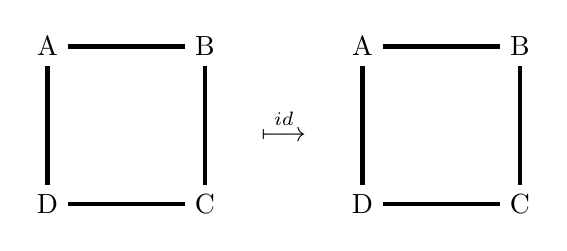
\begin{tikzpicture}
\begin{scope}[shift = {(-4,0)}]
\path (0,2) node (A) {A};
\path (2,2) node (B) {B};
\path (0,0) node (D) {D};
\path (2,0) node (C) {C};
\draw[ultra thick] (A) -- (B) -- (C) -- (D) -- (A);
\node at (3,1) {$\overset{id}{\longmapsto}$};
\end{scope}
\path (0,2) node (A) {A};
\path (2,2) node (B) {B};
\path (0,0) node (D) {D};
\path (2,0) node (C) {C};
\draw[ultra thick] (A) -- (B) -- (C) -- (D) -- (A);
\end{tikzpicture}

\[id = \ptx{cccc}{A & B & C & D\\ A & B & C & D}\]
\end{multicols}

\begin{multicols}{2}%\rho_1
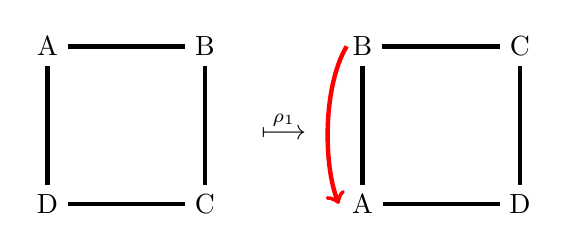
\begin{tikzpicture}
\begin{scope}[shift = {(-4,0)}]
\path (0,2) node (A) {A};
\path (2,2) node (B) {B};
\path (0,0) node (D) {D};
\path (2,0) node (C) {C};
\draw[ultra thick] (A) -- (B) -- (C) -- (D) -- (A);
\node at (3,1) {$\overset{\rho_1}{\longmapsto}$};
\end{scope}
\draw[ultra thick, red, ->] (-0.2,2) .. controls (-0.5,1.5) and (-0.5,0.5) ..  (-0.3,0);
\path (0,2) node (A) {B};
\path (2,2) node (B) {C};
\path (0,0) node (D) {A};
\path (2,0) node (C) {D};
\draw[ultra thick] (A) -- (B) -- (C) -- (D) -- (A);
\end{tikzpicture}

\[\rho_1 = \ptx{cccc}{A & B & C & D\\ D & A & B & C}\]
\end{multicols}

\begin{multicols}{2} %\rho_2
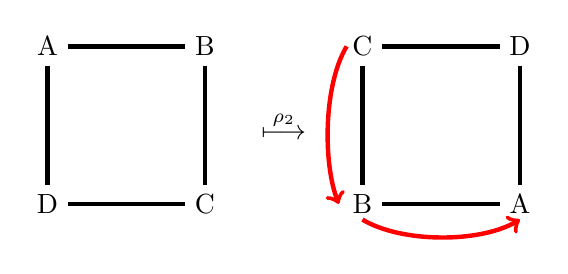
\begin{tikzpicture}
\begin{scope}[shift = {(-4,0)}]
\path (0,2) node (A) {A};
\path (2,2) node (B) {B};
\path (0,0) node (D) {D};
\path (2,0) node (C) {C};
\draw[ultra thick] (A) -- (B) -- (C) -- (D) -- (A);
\node at (3,1) {$\overset{\rho_2}{\longmapsto}$};
\end{scope}
\draw[ultra thick, red, ->] (-0.2,2) .. controls (-0.5,1.5) and (-0.5,0.5) ..  (-0.3,0);
\draw[ultra thick, red, ->] (0,-0.2) .. controls (0.5,-0.5) and (1.5,-0.5) ..  (2, -0.2);
\path (0,2) node (A) {C};
\path (2,2) node (B) {D};
\path (0,0) node (D) {B};
\path (2,0) node (C) {A};
\draw[ultra thick] (A) -- (B) -- (C) -- (D) -- (A);
\end{tikzpicture}

\[\rho_2 = \ptx{cccc}{A & B & C & D\\ C & D & A & B}\]
\end{multicols}

\begin{multicols}{2}%\rho_3
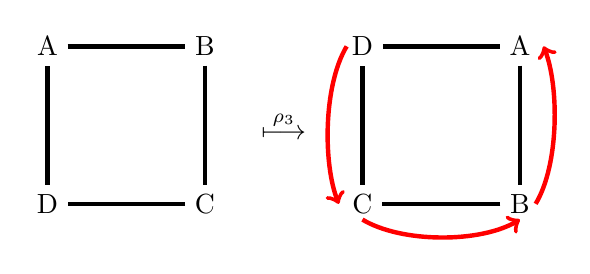
\begin{tikzpicture}
\begin{scope}[shift = {(-4,0)}]
\path (0,2) node (A) {A};
\path (2,2) node (B) {B};
\path (0,0) node (D) {D};
\path (2,0) node (C) {C};
\draw[ultra thick] (A) -- (B) -- (C) -- (D) -- (A);
\node at (3,1) {$\overset{\rho_3}{\longmapsto}$};
\end{scope}
\draw[ultra thick, red, ->] (-0.2,2) .. controls (-0.5,1.5) and (-0.5,0.5) ..  (-0.3,0);
\draw[ultra thick, red, ->] (0,-0.2) .. controls (0.5,-0.5) and (1.5,-0.5) ..  (2, -0.2);
\draw[ultra thick, red, <-] (2.3,2) .. controls (2.5,1.5) and (2.5,0.5) ..  (2.2,0);
\path (0,2) node (A) {D};
\path (2,2) node (B) {A};
\path (0,0) node (D) {C};
\path (2,0) node (C) {B};
\draw[ultra thick] (A) -- (B) -- (C) -- (D) -- (A);
\end{tikzpicture}

\[\rho_3 = \ptx{cccc}{A & B & C & D\\ B & C & D & A}\]
\end{multicols}

\begin{multicols}{2}%\simga_1
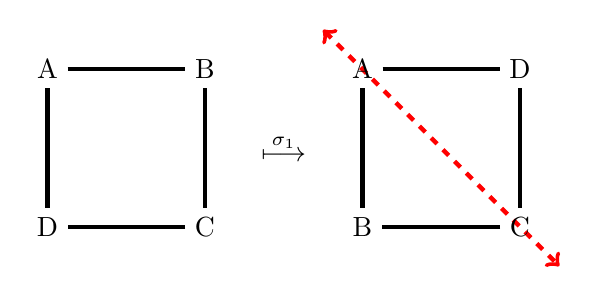
\begin{tikzpicture}
\begin{scope}[shift = {(-4,0)}]
\path (0,2) node (A) {A};
\path (2,2) node (B) {B};
\path (0,0) node (D) {D};
\path (2,0) node (C) {C};
\draw[ultra thick] (A) -- (B) -- (C) -- (D) -- (A);
\node at (3,1) {$\overset{\sigma_1}{\longmapsto}$};
\end{scope}
\draw[ultra thick, red, <->, dashed] (-0.5, 2.5) -- (2.5,-0.5); 
\path (0,2) node (A) {A};
\path (2,2) node (B) {D};
\path (0,0) node (D) {B};
\path (2,0) node (C) {C};
\draw[ultra thick] (A) -- (B) -- (C) -- (D) -- (A);
\end{tikzpicture}

\[\sigma_1 = \ptx{cccc}{A & B & C & D\\ A & D & C & B}\]
\end{multicols}

\begin{multicols}{2}%\sigma_2
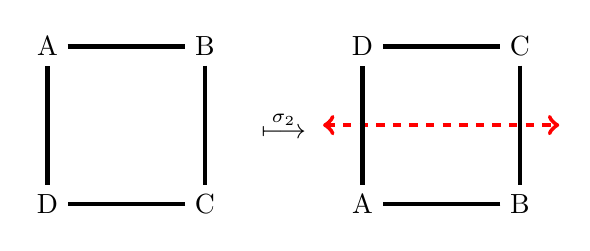
\begin{tikzpicture}
\begin{scope}[shift = {(-4,0)}]
\path (0,2) node (A) {A};
\path (2,2) node (B) {B};
\path (0,0) node (D) {D};
\path (2,0) node (C) {C};
\draw[ultra thick] (A) -- (B) -- (C) -- (D) -- (A);
\node at (3,1) {$\overset{\sigma_2}{\longmapsto}$};
\end{scope}
\draw[ultra thick, red, <->, dashed] (-0.5,1) -- (2.5,1); 
\path (0,2) node (A) {D};
\path (2,2) node (B) {C};
\path (0,0) node (D) {A};
\path (2,0) node (C) {B};
\draw[ultra thick] (A) -- (B) -- (C) -- (D) -- (A);
\end{tikzpicture}

\[\sigma_2 = \ptx{cccc}{A & B & C & D\\ D & C & B & A}\]
\end{multicols}

\begin{multicols}{2} %\sigma_3
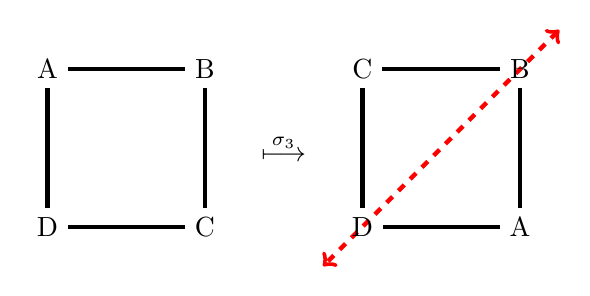
\begin{tikzpicture}
\begin{scope}[shift = {(-4,0)}]
\path (0,2) node (A) {A};
\path (2,2) node (B) {B};
\path (0,0) node (D) {D};
\path (2,0) node (C) {C};
\draw[ultra thick] (A) -- (B) -- (C) -- (D) -- (A);
\node at (3,1) {$\overset{\sigma_3}{\longmapsto}$};
\end{scope}
\draw[ultra thick, red, <->, dashed] (2.5, 2.5) -- (-0.5,-0.5); 
\path (0,2) node (A) {C};
\path (2,2) node (B) {B};
\path (0,0) node (D) {D};
\path (2,0) node (C) {A};
\draw[ultra thick] (A) -- (B) -- (C) -- (D) -- (A);
\end{tikzpicture}

\[\sigma_3 = \ptx{cccc}{A & B & C & D\\ C & B & A & D}\]
\end{multicols}

\begin{multicols}{2}%\sigma_4
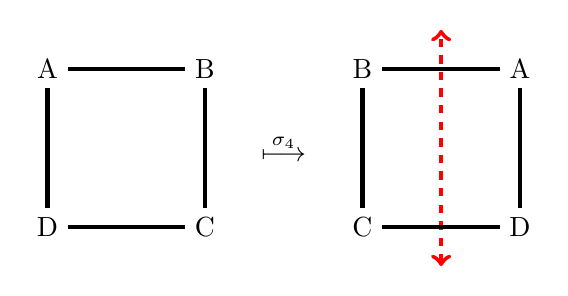
\begin{tikzpicture}
\begin{scope}[shift = {(-4,0)}]
\path (0,2) node (A) {A};
\path (2,2) node (B) {B};
\path (0,0) node (D) {D};
\path (2,0) node (C) {C};
\draw[ultra thick] (A) -- (B) -- (C) -- (D) -- (A);
\node at (3,1) {$\overset{\sigma_4}{\longmapsto}$};
\end{scope}
\draw[ultra thick, red, <->, dashed] (1, -0.5) -- (1,2.5); 
\path (0,2) node (A) {B};
\path (2,2) node (B) {A};
\path (0,0) node (D) {C};
\path (2,0) node (C) {D};
\draw[ultra thick] (A) -- (B) -- (C) -- (D) -- (A);
\end{tikzpicture}

\[\sigma_4 = \ptx{cccc}{A & B & C & D\\ B & A & D & C}\]
\end{multicols}

Multiplication of symmetries is the same permutation multiplication that we introduced earlier. For example,
\[\rho_1\sigma_2 = \ptx{cccc}{A & B & C & D\\ D & A & B & C}\ptx{cccc}{A & B & C & D\\ D & C & B & A} = \ptx{cccc}{A & B & C & D\\ D & C & B & A \\ C & B & A & D} = \sigma_3 \]
and
\[\sigma_4\sigma_1 = \ptx{cccc}{A & B & C & D\\ B & A & D & C}\ptx{cccc}{A & B & C & D\\ A & D & C & B} = \ptx{cccc}{A & B & C & D\\ A & D & C & B \\ B & C & D & A} = \rho_3\]

In this group, $id$ is the identity element, and $\rho_1^{-1} = \rho_3$ while every other element is its own inverse. This group is non-Abelian. The Cayley table for $D_4$ is provided below.

\begin{center}
  \begin{tabular}{c|cccccccc}
    & $id$ & $\rho_1$ & $\rho_2$ & $\rho_3$ & $\sigma_1$ & $\sigma_2$ & $\sigma_3$ & $\sigma_4$ \\
\hline
  $id$ & $id$ & $\rho_1$ & $\rho_2$ & $\rho_3$ & $\sigma_1$ & $\sigma_2$ & $\sigma_3$ & $\sigma_4$ \\
  $\rho_1$ & $\rho_1$ & $\rho_2$ & $\rho_3$ & $id$ & $\sigma_2$ & $\sigma_3$ & $\sigma_4$ & $\sigma_1$ \\
  $\rho_2$ & $\rho_2$ & $\rho_3$ & $id$ & $\rho_1$ & $\sigma_3$ & $\sigma_4$ & $\sigma_1$ & $\sigma_2$ \\
  $\rho_3$ & $\rho_3$ & $id$ & $\rho_1$ & $\rho_2$ & $\sigma_4$ & $\sigma_1$ & $\sigma_2$ & $\sigma_3$ \\
  $\sigma_1$ & $\sigma_1$ & $\sigma_4$ & $\sigma_3$ & $\sigma_2$ & $id$ & $\rho_3$ & $\rho_2$ & $\rho_1$ \\
  $\sigma_2$ & $\sigma_2$ & $\sigma_1$ & $\sigma_4$ & $\sigma_3$ & $\rho_1$ & $id$ & $\rho_3$ & $\rho_2$ \\
  $\sigma_3$ & $\sigma_3$ & $\sigma_2$ & $\sigma_1$ & $\sigma_4$ & $\rho_2$ & $\rho_1$ & $id$ & $\rho_3$ \\
  $\sigma_4$ & $\sigma_4$ & $\sigma_3$ & $\sigma_2$ & $\sigma_1$ & $\rho_3$ & $\rho_2$ & $\rho_1$ & $id$ \\
  \end{tabular}
\end{center}
\end{Exam}

\vfill
\stepcounter{footnote}\footnotetext{See \href{http://abstract.ups.edu/aata/groups-section-mod-n-sym.html}{\S 3.1 Integer Equivalence Classes and Symmetries} and \href{http://abstract.ups.edu/aata/groups-section-defnitions.html}{\S 3.2 Definitions and Examples} in Judson's \href{https://judsonbooks.org/aata/}{Abstract Algebra: Theory and Applications} for additional reading.}
\pagebreak

\startExercises{cayley}

For Exercises \ref{exer:cayleytable:start}--\ref{exer:cayleytable:stop}, determine whether the given Cayley table defined over $G=\{a,b,c,d\}$ forms a group. 
\begin{enumerate}[!HW!]
\begin{multicols}{4}
\item\label{exer:cayleytable:start} \mbox{}\\

\vspace{-25pt}\begin{tabular}{c|cccc}
$\circ$ & $a$ & $b$ & $c$ & $d$\\\hline
$a$ & $a$ & $c$ & $d$ & $a$\\
$b$ & $b$ & $b$ & $c$ & $d$\\
$c$ & $c$ & $d$ & $a$ & $b$\\
$d$ & $d$ & $a$ & $b$ & $c$
\end{tabular}

\item \mbox{}\\

\vspace{-25pt}\begin{tabular}{c|cccc}
$\circ$ & $a$ & $b$ & $c$ & $d$\\\hline
$a$ & $a$ & $b$ & $c$ & $d$\\
$b$ & $b$ & $a$ & $d$ & $c$\\
$c$ & $c$ & $d$ & $a$ & $b$\\
$d$ & $d$ & $c$ & $b$ & $a$
\end{tabular}

\item \mbox{}\\

\vspace{-25pt}\begin{tabular}{c|cccc}
$\circ$ & $a$ & $b$ & $c$ & $d$\\\hline
$a$ & $a$ & $b$ & $c$ & $d$\\
$b$ & $b$ & $c$ & $d$ & $a$\\
$c$ & $c$ & $d$ & $a$ & $b$\\
$d$ & $d$ & $a$ & $b$ & $c$
\end{tabular}

\item\label{exer:cayleytable:stop} \mbox{}\\

\vspace{-25pt}\begin{tabular}{c|cccc}
$\circ$ & $a$ & $b$ & $c$ & $d$\\\hline
$a$ & $a$ & $b$ & $c$ & $d$\\
$b$ & $b$ & $a$ & $c$ & $d$\\
$c$ & $c$ & $b$ & $a$ & $d$\\
$d$ & $d$ & $d$ & $b$ & $c$
\end{tabular}
\end{multicols}
\end{enumerate}\vs


For Exercises \ref{exer:drawcayleytable:start}--\ref{exer:drawcayleytable:stop}, determine the Cayley table for the given group.
\begin{enumerate}[!HW!]
\item \label{exer:drawcayleytable:start} The symmetry group of a rectangle (which is not a square).
\item  The symmetry group of a rhombus (which is not a square).
\begin{multicols}{2}
\item $(\Z_4,+)$
\item\label{exer:drawcayleytable:stop} $(\Z_{12}^*,\cdot)$
\end{multicols}
\end{enumerate}\vs

\textbf{\color{cyan} (Pick 1 from Exercises \ref{exer:cayleycounter:start}-\ref{exer:cayleycounter:stop})}
\begin{enumerate}[!HW!]
\item\label{exer:cayleycounter:start} Prove or disprove that every group containing six elements is abelian.
\item\label{exer:cayleycounter:stop} Give an example of three different groups with eight elements. Why are the groups different?
\end{enumerate}
\vfill
\pagebreak


%%%%%%%%%%%% Section 2.3 %%%%%%%%%%%%%%%%%%%%%%%%%%%%%%%%%%%%%%%%%%%%%%%%%%%%%%%%%%
%%%%%%%%%%%%%%%%%%%%%%%%%%%%%%%%%%%%%%%%%%%%%%%%%%%%%%%%%%%%%%%%%%%%%%%%%%%%
\begin{center} 
\emph{``Never doubt that a small group of thoughtful, committed citizens can change the world; indeed, it's the only thing that ever has.'' -- Margaret Mead}
\end{center}

\begin{Videos}
\video{https://youtu.be/lkjykXnUqCY}{Order of a Group} &
\video{https://youtu.be/Pj-yLgjoD94}{Uniqueness of Identities\\ and Inverses}  &
\video{https://youtu.be/6kmhKE6KWjo}{The Cancellation Laws} &
\video{https://youtu.be/pwwfIm5iKxE}{Exponent Laws}
\end{Videos}

\sectionlabel{Properties of Groups}{groupprop}

\begin{Def} The \textbf{order} of a group $(G, \circ)$ is the cardinality of the set $|G|$.
\end{Def}\vs

\begin{Exam} The group $\Z_n$ under addition has order $|\Z_n| = n$ and the group $S_n$ has order $|S_n|=n!$. These are both examples of \textbf{finite groups}. The groups $\N$, $\Z$, $\Q$, $\R$, and $\C$ under addition are all examples of groups with infinite order, which we call \textbf{infinite groups}.
\end{Exam}\vs

We will now prove some very important properties about all groups. When working with generic groups multiplicative structure is used almost always. For example, we will denote $g\circ h$ in $G$ simplify as $gh$ and the inverse of $g$ as $g^{-1}$. Also, we will use exponential notation to represent iterated products: $g^n = \underbrace{g\cdot g\cdots g}_{n \text{ times}}$ and $g^{-n} = \underbrace{g^{-1}\cdot g^{-1}\cdots g^{-1}}_{n \text{ times}}$. Although we will primarily use $e$ for the identity of $G$, we might sometimes use $1\in G$ as the identity element. In fact, we are justified in saying ``the'' identity elements because it is unique.

\begin{Prop} The identity element in a group $G$ is unique; that is, there exists only one element $e \in G$ such that $eg = ge = g$ for all $g \in G$.\end{Prop}
\begin{pf} Let $e', e''\in G$ such that $ge' = e'g = g$ and $ge'' = e''g= g$ for all $g\in G$. Then 
\[e' = e'e'' = e''.\qedhere\]
\end{pf}\vs

Likewise, we can say ``the'' inverse of $g\in G$ since inverses are also unique.

\begin{Prop} If $g$ is any element in a group $G$, then the inverse of $g$ is unique. \end{Prop}
\begin{pf} Let $g', g''\in G$ such that $gg' = g'g = e$ and $gg'' = g''g= e$. Then 
\[g' = g'e = g'(gg'') = (g'g)g'' = eg'' = g''.\qedhere\]
\end{pf}\vs

\begin{Prop} Let $G$ be a group. For any $g, h\in G$, then $(gh)^{-1} = h^{-1}g^{-1}$. \end{Prop}
\begin{pf} Since inverses are unique in groups, as shown above, it suffices to show that $h^{-1}g^{-1}$ acts like an inverse to $(gh)^{-1}$. If $h^{-1}g^{-1}$ does act like an inverse to $(gh)^{-1}$ then uniqueness of inverses demand that $(gh)^{-1} = h^{-1}g^{-1}$. Note that 
\[(gh)(h^{-1}g^{-1}) = g(hh^{-1})g^{-1} = g(e)g^{-1} = gg^{-1} = e.\] Similarly, $(h^{-1}g^{-1})(gh) = e$. Therefore, $h^{-1}g^{-1}$ is the inverse of $gh$.
\end{pf}\vs

\begin{Prop} Let $G$ be a group. For any $g\in G$, $(g^{-1})^{-1} = g$.\end{Prop}
\begin{pf} Since inverses are unique in groups, as shown above, it suffices to show that $g$ acts like an inverse to $g^{-1}$, like the previous proof.  Note that 
\[gg^{-1} = e = g^{-1}g.\]  
 Therefore, $g$ is the inverse of $g^{-1}$.
\end{pf}\vs

\begin{Prop}[Cancellation Laws]\label{prop:cancel} If $G$ is a group and $a, b, c \in G$, then $ab = ac$ implies $b = c$ and  $ba = ca$ implies $b = c$.\end{Prop}
\begin{pf} We will prove the case that $ab=ac$ implies that $b=c$.  Multiplying both sides of the equation on the left by $a^{-1}$ then gives 
\[a^{-1}(ab) = a^{-1}(ac)\qRightarrow (a^{-1}a)b = (a^{-1}a)c \qRightarrow eb = ec\qRightarrow b= c.\]
The case of $ba=ca$ is handled similarly.
\end{pf}\vs

This proposition tells us that the \textbf{right} and \textbf{left cancellation laws} are true in all groups. In fact, the above proof used all three axioms of group theory: associativity, identity, and inverses, to prove the cancellation laws. In some regard, any algebraic object with cancellation must be group-like. 

\begin{Prop}\label{prop:uniquesoln} Let $G$ be a group and $a, b \in G$. Then the equations $ax = b$ and $xa = b$ have unique solutions in $G$.\end{Prop}
\begin{pf} We will prove the case that $ax=b$ has a unique solution in $G$. Note that $x=a^{-1}b$ is a solution the equation since 
\[a(a^{-1}b) = (aa^{-1})b = eb = b.\] This shows existence of a solution. For uniqueness, if $x$ and $y$ are both solutions to the above equation, then $ax = b = ay$. Canceling $a$ on the left gives $x=y$. Thus, $ax=b$ has a unique solution in $G$. The case of $xa=b$ is handled similarly.
\end{pf}\vs

Again, we should emphasize that in the above proof we used all three axioms of group theory to solve equations. Groups are exactly the setting where we solve equations in the manner we first learned in algebra class.

\begin{Prop}[Exponential Laws]\label{prop:explaws} In a group $G$, the usual exponent laws hold; that is, for all $g, h\in G$ and $m, n\in \Z$,
\begin{enumerate}[!THM!, start=1]
\item $g^mg^n = g^{m+n}$
\item $(g^m)^n = g^{mn}$
\item $(gh)^n = (h^{-1}g^{-1})^{-n}$. Furthermore, if $G$ is Abelian, then $(gh)^n = g^nh^n$.
\end{enumerate}
\end{Prop}\vs

The proof of the above exponent laws follows from the associativity of the group and an (double) induction argument. It should be emphasized that, in general, $(gh)^n \neq g^nh^n$ in groups and commutativity in some form is needed for equality.\\

In fact, when a group is Abelian, additive notation is often used instead of multiplicative notation.  For example, we will denote $g\circ h$ in $G$ simplify as $g+h$ and the inverse of $g$ as $-g$. Also, we will use multiplicative notation to represent iterated products: $ng = \underbrace{g+ g+\ldots + g}_{n \text{ times}}$ and $-ng = \underbrace{-g + -g+\ldots + -g}_{n \text{ times}}$. Although we will primarily use $e$ for the identity of $G$, we might sometimes use $0\in G$ as the identity element. The three ``exponent laws'' look like distributive laws for additive groups: for $g,h\in G$ and $m,n\in \Z$, we have
\begin{enumerate}[!THM!, start=1]
\item $mg+ng = (m+n)g$
\item $m(ng) = (mn)g$
\item $m(g+h) = mg+mh$.
\end{enumerate}\vs



\vfill
\stepcounter{footnote}\footnotetext{See \href{http://abstract.ups.edu/aata/groups-section-defnitions.html}{\S 3.2 Definitions and Examples} in Judson's \href{https://judsonbooks.org/aata/}{Abstract Algebra: Theory and Applications} for additional reading.}
\pagebreak

\startExercises{groupprop}

For Exercises \ref{exer:groupprop:start}--\ref{exer:groupprop:stop}, prove the given statement about a group $G$.\\
\textbf{\color{cyan} (Pick 3 from Exercises \ref{exer:groupprop:start}-\ref{exer:groupprop:pickstop}; Pick 2 from Exercises \ref{exer:groupprop:pickstart}-\ref{exer:groupprop:stop})}
\begin{enumerate}[!HW!]
\item \label{exer:groupprop:start} For any $g_1,g_2,\ldots, g_n\in G$, $(g_1g_2\cdots g_n)^{-1} =g_n^{-1}\cdots g_2^{-1}g_1^{-1}$.
\item For any $a,b,c\in G$, if $ba=ca$, then $b=c$ (the remaining part of \propref{prop:cancel}).
\item For any $a,b\in G$, the equation $xa=b$ has a unique solution in $G$ (the remaining part of \propref{prop:uniquesoln}).
\item \propref{prop:explaws}
\item \label{exer:groupprop:pickstop} If $a^2=e$ for all $a\in G$, then $G$ is abelian.
\item \label{exer:groupprop:pickstart} If $(ab)^2=a^2b^2$ for all $a, b\in G$, then $G$ is abelian.
\item If $ab=a^{-1}b^{-1}$ for all $a, b\in G$, then $G$ is abelian.
\item\label{exer:a4b=ba} For $a,b\in G$, if $a^4b=ba$ and $a^3=e$, then $ab=ba$.
\item\label{exer:groupprop:stop}   If $|G|$ is even, then there exists some nonidentity $g\in G$ such that $g^2=e$.
\end{enumerate}

\pagebreak

%%%%%%%%%%%% Section 2.4 %%%%%%%%%%%%%%%%%%%%%%%%%%%%%%%%%%%%%%%%%%%%%%%%%%%%%%%%%%
%%%%%%%%%%%%%%%%%%%%%%%%%%%%%%%%%%%%%%%%%%%%%%%%%%%%%%%%%%%%%%%%%%%%%%%%%%%%
\begin{center}\emph{``Someone who hates one group will end up hating everyone -- and, ultimately, hating himself or herself.''\\ -- Elie Wiesel}
\end{center}

\begin{Videos}
\video{https://youtu.be/DYO43qzn1zs}{Subgroups} &
\video{https://youtu.be/y40NWogswzU}{Not Every Subset\\ is a Subgroup}  &
\video{https://youtu.be/RpbKdL40e8w}{A Condition for\\ Checking Subgroups} &
\video{https://youtu.be/sMVyDmNB5mY}{Examples of\\ Subgroups} &
\video{https://youtu.be/8VtKk5f1vj0}{Another Condition\\ for Checking\\ Subgroups}
\end{Videos}

\sectionlabel{Subgroups}{subgroup}

\begin{Def} Let $(G,\circ)$ be a group. Let $H\subseteq G$. We say that $(H,\circ)$ is a \textbf{subgroup} of $G$, denoted $H\le G$, if the restriction $\circ : H\times H\to H$ forms a group structure on $(H,\circ)$.
\end{Def}\vs

For any group $G$, $G$ is itself a subgroup, called the \textbf{improper subgroup}. Every other subgroup is called \textbf{proper}. Also, the \textbf{trivial subgroup} $\{e\}$ is also a subgroup of $G$ since $e\circ e = e$. Note that $\emptyset \not\le G$ since $e\notin \emptyset$.

\begin{Exam} With respect to regular addition, we have $\Z \le \Q\le \R\le \C$,  and with respect to regular multiplication, we have $\Q^*\le \R^* \le \C^*$. These are all infinite, Abelian subgroups. \\

On the other hand, the set $H= \{\pm 1, \pm i\}$ is a finite subgroup of $\C^*$ of order 4. Similarly, $\{\pm 1\} \le \R^*$.\\

The dihedral group $D_n$ is a subgroup of the symmetric group $S_n$. These are finite, non-Abelian subgroups. The quaternion group $Q_8$ is a finite, non-abelian subgroup of $\GL_2(\C)$.
\end{Exam}\vs

\begin{Exam} Although $\Z_5 = \{0, 1, 2, 3, 4\} \subseteq \{0, 1, 2, 3, 4, 5\} = \Z_6$, $\Z_5$ is NOT a subgroup of $\Z_6$, that is $\Z_5\not\le \Z_6$. Although $\Z_5$ is a group, this group structure is not formed by restricting the\vspace{-0.15 in}
\begin{multicols}{2}
\noindent   group operation from $\Z_6$, that is, the addition (or multiplication) modulo 5 is NOT formed by restricting addition (or multiplication) modulo 6.  On the other hand, $H=\{0, 2, 4\} \le \Z_6$ since $H$ does form a group structure as illustrated in the Cayley table below. Likewise, $\{0, 3\} \le \Z_6$. Conversely, $\Z_5$ has NO nontrivial, proper subgroups.\columnbreak

\mbox{}\vspace{-25pt}
\begin{center}
  \begin{tabular}{c|ccc}
  $+ \pmod 6$ & 0 & 2 & 4 \\\hline
  0 & 0 & 2 & 4 \\
  2 & 2 & 4 & 0 \\
  4 & 4 & 0 & 2 \\
  \end{tabular}
\end{center}
\end{multicols}
\end{Exam}\vs


\begin{Prop} Let $G$ be a group. A subset $H\subseteq G$ is a subgroup of $G$ if and only if 
\begin{enumerate}[!THM!, start=1]
\item (closure) $gh\in H$ for all $g,h\in H$
\item (identity) $e\in H$
\item (inverses) $h^{-1}\in H$ for all $h\in H$
\end{enumerate}
\end{Prop}
\begin{pf}
Let $H\le G$. Since $H$ is itself a group, the product of any two elements in $H$ must also be an element of $H$. Thus, $H$ is closure under multiplication. Also, $H$ must contain an identity element $e'\in H$ such that $e'h = he' = h$ for all $h\in H$. In particular, this identity holds for $e'$, that is, $e'e'=e'$ in $H$. Since $e'\in G$, it has an inverse in $G$, namely $(e')^{-1}$. Of course, $e = e'(e')^{-1} = (e'e')(e')^{-1} = e'(e'(e'^{-1})) = e'e = e'$. Thus, the identity of $H$ must be the \emph{same identity} as $G$. Finally, each element $h$ of $H$ has an inverse in $H$, call it $h'$, such that, $hh' = h'h= e$. But since the identity of $H$ and $G$ are the same, $h'$ is an inverse of $h$ in $G$. Since inverses in $G$ are unique, we conclude that $h'=h^{-1}$ and $h^{-1}\in H$, that is, $H$ has the \emph{same inverses} as $G$.\\

Conversely, suppose the subset $H$ is closed under the operation and contains the identity and inverses. Since the operation is closed, there is a well-defined binary operation on $H$. Likewise, there is an identity element and each element has a inverse. The last axiom to be a group for $H$ is associativity. Let $g,h,k\in H$. Since $H\subseteq G$, we have that $g,h,k\in G$ and $g(hk) = (gh)k$ in $G$ since it is a group, that is, associativity is \emph{inherited} from $G$. Therefore, $H$ is a group in its own right. 
\end{pf}\vs

In the previous proof, we mentioned that associativity from a group $G$ is inherited by a subset $H$, because if the property holds for all elements of $G$ then certainly it still remains true for the restriction to $H$. This is also true for commutativity, that is, every subgroup of an Abelian group is Abelian, because commutativity of the subset is inherited from the ambient commutative group. On the other hand, not every subgroup of a non-Abelian group has to be non-Abelian (why is that?). While properties like associativity and commutativity are inherited by any closed subset, issues about containment, like containing identity or inverse elements, are not guaranteed. Considering that a subset is likely a collection of $G$ with some missing, we should be highly curious whether the elements omitted from $G$ are products, identities, or inverses.

\begin{Exam} Let $n\Z = \{kn \mid k\in \Z\}$, the set of all integers divisible by $n$ (this is, of course, just the congruence class $[0]$ modulo $n$). Then $n\Z \le \Z$.
\begin{pf}
To show closure of the operations, let $a,b\in n\Z$. Then there exists $k, \ell\in \Z$ such that $a=kn$ and $b=\ell n$. Then $a+b = kn + \ell n = (k+\ell)n$ where $k+\ell\in\Z$. Therefore, $a+b\in n\Z$, which shows that $n\Z$ is closed under addition. Of course, $0=0n\in n\Z$. This shows that $n\Z$ contains the identity. Finally, if $a=kn\in \Z$, then $-a = (-k)n\in \Z$. Therefore, $n\Z$ is closed under inverses. This then proves that $n\Z\le \Z$ for all $n\in \Z$.
\end{pf} 
\end{Exam}\vs

\begin{Exam} Let $\SL_n(\R) = \{A\in \GL_n(\R)\mid \det(A)=1\}$, which is called the \textbf{special linear group}. As the name indicates, $\SL_n(\R) \le \GL_n(\R)$.
\begin{pf}
For closure, remember that the determinant as the following useful property: $\det(AB) = \det(A)\det(B)$ for all matrices $A$ and $B$. So, if $A,B\in \SL_n(\R)$, then $\det(A) = \det(B) = 1$ and 
\[\det(AB) = \det(A)\det(B) = 1\cdot 1 = 1.\] Thus, $AB\in \SL_n(\R)$ and it is closed under multiplication. Of course, $\det(I_n) =1$, so $I_n\in \SL_n(\R)$. Finally, \[\det(A^{-1}) = 1\cdot \det(A^{-1}) = \det(A)\det(A^{-1}) = \det(AA^{-1}) = \det(I_n) = 1.\] Thus, $A^{-1}\in \SL_n(\R)$. Therefore, $\SL_n(\R)$ is a subgroup of $\GL_n(\R)$. 
\end{pf} 
\end{Exam}\vs

\begin{Prop} Let $H$ be a subset of a group $G$. Then $H$ is a subgroup of $G$ if and only if $H\neq \emptyset$ and $gh^{-1}\in H$ for all $g,h\in H$.
\end{Prop}
\begin{pf} 
If $H$ is a subgroup, then $H\neq \emptyset$ since $e\in H$. Likewise, if $g,h\in H$, then $h^{-1}\in H$ and $gh^{-1}\in H$.\\

Conversely, suppose that $H\neq\emptyset$ and $gh^{-1}\in H$ for all $g, h \in H$. Let $h\in H$, where such an element exists since $H\neq \emptyset$. Then $e = hh^{-1} \in H$. So, $H$ contains the identity. Likewise, $h^{-1} = eh^{-1} \in H$. Thus, $H$ is closed under inversion. Finally, if $g,h\in H$, then $h^{-1}\in H$ and $gh = g(h^{-1})^{-1}\in H$. Thus, $H$ is closed under multiplication. This shows that $H$ is a subgroup.
\end{pf}\vs

\vfill
\stepcounter{footnote}\footnotetext{See \href{http://abstract.ups.edu/aata/groups-section-subgroups.html}{\S 3.3 Subgroups} in Judson's \href{https://judsonbooks.org/aata/}{Abstract Algebra: Theory and Applications} for additional reading.}
\pagebreak

\startExercises{subgroup}

For Exercises \ref{exer:subgroup:start}--\ref{exer:subgroup:stop}, prove the given subset is a subgroup of the given group.\\
\textbf{\color{cyan} (Pick 3 from Exercises \ref{exer:subgroup:start}-\ref{exer:subgroup:stop})}
\begin{enumerate}[!HW!]
\item \label{exer:subgroup:start} $H=\{2^k\mid k\in \Z\} \subseteq \Q^*$
\item $S^1=\{z\in \C^*\mid |z|=1\}\subseteq \C^*\}$
\item\label{exer:subgroup:quadratic} $H=\{a+b\sqrt{2}\mid a, b\in \Q\} \subseteq \R^*$
\item $H = \left\{\ptx{cc}{\cos\theta&-\sin\theta\\\sin\theta&\cos\theta}\ \middle|\ \theta\in \R\right\}\subseteq \SL_2(\R)$
\item $H=\left\{\ptx{cc}{a&b\\c&d}\ \middle|\ a,b,c,d\in \R, a+d=0\right\}\footnote{In this exercise, $H$ is the set of \textbf{traceless matrices}. Recall that the \textbf{trace} of a square matrix is the sum of its diagonal entries.} \subseteq M_{2\times 2}(\R) := \left\{\ptx{cc}{a&b\\c&d}\ \middle|\ a,b,c,d\in \R\right\}$
\item \label{exer:subgroup:stop} $\SL_2(\Z)\subseteq \SL_2(\R)$
\end{enumerate}\vs

For Exercises \ref{exer:subgroupproof:start}--\ref{exer:subgroupproof:stop}, let $H, K\le G$. Prove the given statement.\\
\textbf{\color{cyan} (Pick 2 from Exercises \ref{exer:subgroupproof:start}-\ref{exer:subgroupproof:stop})}
\begin{enumerate}[!HW!]
\item \label{exer:subgroupproof:start} $H\cap K\le G$, that is, the intersection of any two subgroups is itself a subgroup.
\item\label{exer:subgroup:union} There exists a group $G$ with subgroups $H$, $K$ such that $H\cup K$ is  not a subgroup of $G$, that is, the union of two subgroups is not necessarily a subgroup.
\item There exists a group $G$ with subgroups $H$, $K$ such that $HK :=\{hk\mid h\in H, k\in K\}$ is  not a subgroup of $G$, that is, the product of two subgroups is not necessarily a subgroup.

\begin{Def}\label{def:center} The \textbf{center} of a group $G$, denoted $Z(G)$, is defined as 
\[Z(G) := \{z\in G\mid zg=gz\ \text{for all}\ g\in G\}.\]
\end{Def}\vs
\item  For any group $G$, $Z(G)\le G$.

\begin{Def}\label{def:central:subroup} The \textbf{centralizer} of a subgroup $H$, denoted $C_G(H)$, is defined as 
\[C_G(H) := \{z\in G\mid zh=hz\ \text{for all}\ h\in H\}.\footnotemark\]
\end{Def}\vs

\item \label{exer:subgroupproof:stop}  For any group $G$ and subgroup $H$, $C_G(H)\le G$.
\end{enumerate}
\vfill

\footnotetext{Note that $C_G(G) = Z(G)$.}
\pagebreak

%%%%%%%%%%%% Section 2.5 %%%%%%%%%%%%%%%%%%%%%%%%%%%%%%%%%%%%%%%%%%%%%%%%%%%%%%%%%%
%%%%%%%%%%%%%%%%%%%%%%%%%%%%%%%%%%%%%%%%%%%%%%%%%%%%%%%%%%%%%%%%%%%%%%%%%%%%
\begin{center}
\emph{``A team will always appreciate a great individual if he's willing to sacrifice for the group.''\\ -- Kareem Abdul-Jabbar}
\end{center}

\begin{Videos}
\video{https://youtu.be/zgsTzu4zey4}{Partially Ordered Sets} &
\video{https://youtu.be/jd2dDg1Kqm0}{Hasse Diagrams}  &
\video{https://youtu.be/UVw98SPcp2o}{Direct Products} 
\end{Videos}

\sectionlabel{Hasse Diagrams}{hasse}

\begin{Def} A \textbf{partial order} $\preceq$ on a set $X$ is a relation $\preceq \subseteq X\times X$ such that 
\begin{enumerate}[!THM!,start=1]
\item (Reflexive property) $x\preceq x$ for all $x\in X$;
\item (Antisymmetric property) if $x\preceq y$ and $y \preceq x$ then implies $x=y$;
\item (Transitive property) If $x\preceq y$ and $y\preceq z$, then $x\preceq z$.
\end{enumerate}
A set $X$ equipped with a partial order $\preceq$ is called a \textbf{partially ordered set} (or \text{poset}). For elements $x, y\in X$, we say that $x$ and $y$ are \textbf{comparable} if $x\preceq y$ (or $y\preceq x$).
\end{Def}\vs

\begin{Exam} We say that $a\le b$ for $a,b\in \R$ (or $\Q, \Z, \N$) if $b-a$ is nonnegative. This provides the usual ordering of $\R$ which is a partial ordering. 
\end{Exam}\vs

\begin{Exam} Let $X$ be any set. Then $\P(X)$ (or $2^X$) denotes the \textbf{power set} of $X$, which is the set of all subsets of $X$. Then $(\P(X), \subseteq)$ is a partially ordered set. Let $A, B, C \subseteq X$.
\begin{pf}
\begin{enumerate}[!THM!,start=1]
\item (Reflexive property) If $x\in A$, then $x\in A$. Therefore, $A\subseteq A$.
\item (Antisymmetry property) Let $A\subseteq B$ and $B\subseteq A$. Then each of the two sets contain the same elements and $A=B$.
\item (Transitive property) Let $A\subseteq B$ and $B\subseteq C$. Let $x\in A$. Then $x\in B$, which also implies that $x\in C$. Thus, $A\subseteq C$.
\end{enumerate}
Therefore, $\subseteq$ is a partial ordering. 
\end{pf}
\end{Exam}\vs

The reason that this kind of ordering is called \emph{partial} is because not all elements are comparable. For example, let $X = \{1,2,3\}$, $Y=\{1\}$, and $Z=\{2\}$. Then $Y, Z\subseteq X$ but $Z\not\subseteq Y$ nor $Y\not\subseteq Z$. Thus, only some of the elements of $\P(X)$ are ordered.

\begin{Exam} Let $G$ be a group. Then the set of all subgroups of $G$ forms a partially ordered set under $\le$. The proof of this fact is similar to the previous example.\end{Exam}\vs

\begin{Exam} Let $n \in \Z^+$. Let $X$ be the set of all positive divisors of $n$. Then $(X,\mid)$ is a partially ordered set with respect to divisibility. This proof is an exercise for the reader.\end{Exam}\vs

\begin{Def} A \textbf{Hasse diagram} (or \textbf{lattice diagram}) of a partially ordered set $(X,\preceq)$ is a graph whose vertices are the elements of $X$ and for which an edge $(x,y)$ exists if $x\preceq y$ and whenever $x\preceq z\preceq y$ either $z=x$ or $z=y$.
\end{Def}\vs

\begin{Exam} 
\begin{multicols}{2}
 Let $X=\{a,b,c\}$. Then the Hasse diagram for the partially ordered set $\P(X)$ is given below.\\

Because of the transitivity of the ordering, any path upward the graph demonstrates comparability of subsets. For example, $\{a\} \subseteq \{a, b, c\}$ since $\{a\} \subseteq \{a, b\} \subseteq \{a, b, c\}$.

\begin{center}
\begin{tikzpicture}
\node (0) at (0,0) {$\emptyset$};
\node (a) at ($ (0) +(-1.5,1.5) $) {$\{a\}$};
\node (b) at ($ (0) +(0,1.5) $) {$\{b\}$};
\node (c) at ($ (0) +(1.5,1.5) $) {$\{c\}$};
\node (ab) at ($ (a) +(0,1.5) $) {$\{a, b\}$};
\node (ac) at ($ (b) +(0,1.5) $) {$\{a, c\}$};
\node (bc) at ($ (c) +(0,1.5) $) {$\{b,c\}$};
\node (abc) at ($(ac) +(0,1.5) $) {$\{a,b,c\}$};

\draw[very thick] (0) -- (a) -- (ab) -- (abc) -- (bc) -- (c) -- (0) -- (b) -- (ab) (b) -- (bc) (a) -- (ac) -- (c) (ac) -- (abc);
\end{tikzpicture}
\end{center}
\end{multicols}
\end{Exam}\vs

\begin{Exam} \begin{multicols}{2}The Hasse diagram for the subgroups of $\Z_{6}$ is displayed below.
\begin{center}
\begin{tikzpicture}
\node (1) at (0,0) {$\{0\}$};
\node (2) at ($ (1) +(-1,1.5) $) {$\{0, 3\}$};
\node (3) at ($ (1) +(1, 1.5) $) {$\{0, 2, 4\}$};
\node (6) at ($(1) +(0,3) $) {$\Z_{6}$};

\draw[very thick] (1) -- (2) -- (6) -- (3) -- (1);
\end{tikzpicture}
\end{center}
\end{multicols}
\end{Exam}\vs

\begin{Exam} 
\begin{multicols}{2}
The Hasse diagram for the subgroups of $\Z_{24}$ is displayed below. It can be verified that each of the subsets is a subgroup of $\Z_{24}$.\columnbreak

\mbox{}\hspace{-80pt}
\begin{tikzpicture}
\node (1) at (0,0) {$\{0\}$};
\node (2) at ($ (1) +(-3,1.5) $) {$\{0, 12\}$};
\node (3) at ($ (1) +(3,1.5) $) {$\{0, 8, 16\}$};
\node (4) at ($ (2) +(0,1.5) $) {$\{0, 6, 12, 18\}$};
\node (6) at ($ (3) +(0,1.5) $) {$\{0, 4, 8, 12, 16, 20\}$};
\node (8) at ($ (4) +(0,1.5) $) {$\{0, 3, 6, 9, 12, 15, 18, 21\}$};
\node (12) at ($ (6) +(0,1.5) $) {$\{0, 2, 4, 6, 8, 10, 12, 14, 16, 18, 20, 22\}$};
\node (24) at ($(1) +(0,6) $) {$\Z_{24}$};
\draw[very thick] (1) -- (2) -- (4) -- (8) -- (24) -- (12) -- (6) -- (3) -- (1) (2) -- (6) (4) -- (12);
\end{tikzpicture}
\end{multicols}
\end{Exam}\vs

\begin{Prop} Let $(G, \circ)$ and $(H, \ast)$ be groups. Then $G\times H$ can be made into a group, called the \textbf{direct product} of $G$ and $H$, using component--wise multiplication, that is, \[(g, h)(g', h') = (g\circ g', h\ast h').\]
\end{Prop}
\begin{pf}
Let $(g,h), (g',h'), (g'',h'')\in G\times H$. Then 
\begin{eqnarray*}
(g,h)[(g',h')(g'',h'')] &=& (g,h)(g'\circ g'', h'\ast h'') = (g \circ (g'\circ g''), h \ast (h'\ast h''))\\
 &=& ((g\circ g')\circ g'', (h\ast h')\ast h'') = (g\circ g', h\ast h')(g'', h'') = [(g,h)(g',h')](g'',h'').
\end{eqnarray*} Therefore, component-wise multiplication is associative. Next, 
\[(e,e)(g,h) = (e\circ g,e\ast h) = (g,h) = (g\circ e,h\ast e) = (g,h)(e,e).\] Thus, $(e,e)$ is the identity of $G\times H$. Finally, 
\[(g^{-1},h^{-1})(g,h) = (g^{-1}\circ g,h^{-1}\ast h) = (e,e) = (g\circ g^{-1},h\ast h^{-1}) = (g,h)(g^{-1},h^{-1}).\] Thus, $(g,h)^{-1} = (g^{-1}, h^{-1})$ and $G\times H$ has inverses. Therefore, $G\times H$ is a group.
\end{pf}\vs

\begin{Exam} 
\begin{multicols}{2}
Consider the group $V_4 = \Z_2\times Z_2 = \{(0,0), (1,0), (0,1), (1,1)\}$, called the \textbf{Klein 4-group}. The Hasse diagram is displayed below. 
\begin{center}
\begin{tikzpicture}
\node (1) at (0,0) {$\{(0,0)\}$};
\node (a) at ($ (1) +(-2.5,1.5) $) {$\{(0,0), (1,0)\}$};
\node (b) at ($ (1) +(0,1.5) $) {$\{(0,0), (1,1)\}$};
\node (c) at ($ (1) +(2.5, 1.5) $) {$\{(0,0), (0,1)\}$};
\node (abc) at ($(1) +(0,3) $) {$V_4$};

\draw[very thick] (1) -- (a) -- (abc) -- (c) -- (1) -- (b) -- (abc);
\end{tikzpicture}
\end{center}
\end{multicols}

\begin{multicols}{2}
Alternatively, the group $\Z_4$ is also an Abelian group of order 4, but the Hasse diagram, displayed below, is very different. This demonstrates that the groups are, in fact, not the same group.

\begin{center}
\begin{tikzpicture}
\node (1) at (0,0) {$\{0\}$};
\node (b) at ($ (1) +(0,1.5) $) {$\{0, 2\}$};
\node (abc) at ($(1) +(0,3) $) {$\Z_4$};

\draw[very thick] (1) -- (b) -- (abc);
\end{tikzpicture}
\end{center}
\end{multicols}
\end{Exam}


\vfill
\stepcounter{footnote}\footnotetext{See \href{http://abstract.ups.edu/aata/groups-section-subgroups.html}{\S 3.3 Subgroups} and  \href{http://abstract.ups.edu/aata/boolean-section-lattices.html}{\S 19.1 Lattices} in Judson's \href{https://judsonbooks.org/aata/}{Abstract Algebra: Theory and Applications} for additional reading.}
\pagebreak

\startExercises{hasse}

\begin{enumerate}[!HW!]
\item Let $n \in \Z^+$. Let $X$ be the set of all positive divisors of $n$. Prove that $(X,\mid)$ is a partially ordered set with respect to divisibility.
\end{enumerate}\vs

For Exercises \ref{exer:poset:start}--\ref{exer:poset:stop}, draw the Hasse diagram for the given partially ordered set.
\begin{enumerate}[!HW!]
\begin{multicols}{2}
\item \label{exer:poset:start} The subsets of $X=\{a,b,c,d\}$
\item The subgroups of $\Z_{12}$
\end{multicols}
\begin{multicols}{2}
\item The subgroups of $\Z_3\times \Z_3$
\item\label{exer:poset:D3} The subgroups of $S_3$
\end{multicols}
\begin{multicols}{2}
\item The subgroups of $D_4$
\item \label{exer:poset:stop} The subgroups of $Q_8$
\end{multicols}
\end{enumerate}
\vfill
\pagebreak


%%%%%%%%%%%% Supplementary Exercises %%%%%%%%%%%%%%%%%%%%%%%%%%%%%%%%%%%%%%%%%%%%%%%%%%%%%%%%%%
%%%%%%%%%%%%%%%%%%%%%%%%%%%%%%%%%%%%%%%%%%%%%%%%%%%%%%%%%%%%%%%%%%%%%%%%%%%%
\startSuppExercises{group}

\begin{enumerate}[!HW!]
\item List all elements of $\Z_4\times \Z_2$.

\item\label{exer:group:noncommutematrix} Given an example of two elements $A$ and $B$ in $\GL_2(\R)$ such that $AB\neq BA$.

\item Prove that the $\det(AB)=\det(A)\det(B)$ holds for all $A,B\in \GL_2(\R)$. Explain from this property that $\GL_2(\R)$ is closed under multiplication and hence a group. Likewise, explain from this property that $\SL_2(\R)\le \GL_2(\R)$.

\item \label{exer:group:noncommutedihedral} Given an example of two elements $g, h\in G$ for some group $G$ and some $n\in \N$ such that $(gh)^n\neq g^nh^n$.

\item \label{exer:group:commutatorpower} Let $G$ be a group and $g, h\in G$. Prove that, for any $n\in \Z$, $(ghg^{-1})^n=gh^ng^{-1}$.

\item If $|G|=2n$, prove that $G$ must have an element of order $2$. 

\item Give an example of an infinite group in which every nontrivial subgroup is infinite.

\item Prove that $G\times H$ is abelian if and only if $G$ and $H$ are abelian.

\item Prove or disprove: Every proper subgroup of a nonabelian group is nonabelian.


\item Let $G$ be a group with $H\le G$. If $g\in G$, let $gHg^{-1} := \{ghg^{-1}\mid h\in H\}$. Prove that $gHg^{-1}\le G$, called the \textbf{conjugate subgroup} of $H$ relative to $g$. 

\item Prove or disprove: The set of all nonzero integers is a poset, where $a\preceq b$ is defined by $a\mid b$.
\begin{Def} 
We say a poset $(X,\preceq)$ is a \textbf{totally ordered set} if for all $x,y\in X$ either $x\preceq y$ or $y\preceq x$.
\end{Def}\vs
\item Is $(\N, \mid)$ a totally ordered set? Why or why not? %No
\item Prove that $\N, \Z, \Q$, and $\R$ are totally ordered sets under the usual ordering $\le$.
\end{enumerate}
\pagebreak


%%%%%%%%%%%% CHAPTER 3 %%%%%%%%%%%%%%%%%%%%
%%%%%%%%%%%%%%%%%%%%%%%%%%%%%%%%%%%%%%%%%%%%%%%%%%%%%%%%%%%%%%%%%%%%%%%%%%%%%%%%
\chapterlabel{Cyclic Groups}{cyclic}\pagebreak

%%%%%%%%%%%% Section 3.1 %%%%%%%%%%%%%%%%%%%%%%%%%%%%%%%%%%%%%%%%%%%%%%%%%%%%%%%%%%
%%%%%%%%%%%%%%%%%%%%%%%%%%%%%%%%%%%%%%%%%%%%%%%%%%%%%%%%%%%%%%%%%%%%%%%%%%%%
\begin{center} 
\emph{``Without forgiveness life is governed by\ldots an endless cycle of resentment and retaliation.''\\ -- Roberto Assagioli}
\end{center}

\begin{Videos}
\video{https://youtu.be/X6-OVRT33u4}{Cyclic Subgroups} &
\video{https://youtu.be/sI-bthTFzxE}{Examples of\\ Cyclic Subgroups}  &
\video{https://youtu.be/HA5MGLoHDpg}{Cyclic Groups} &
\video{https://youtu.be/TNS-2XoPBi4}{Every Subgroup\\ of a Cyclic Group\\ is Cyclic}&
\video{https://youtu.be/8PUfDkRVaiM}{Order of\\ an Element}
\end{Videos}

\sectionlabel{Cyclic Groups}{cyclic}

Often a subgroup will depend entirely on a single element of the group; that is, knowing that particular element will allow us to compute any other element in the subgroup.

\begin{Thm} Let $G$ be a group and let $g\in G$. Then the set 
\[\langle g\rangle = \{g^n\mid n\in \Z\}\footnotemark\]
is an abelian subgroup of $G$, called the \textbf{cyclic subgroup} generated by $g$. In fact, this subgroup is the smallest subgroup containing $g$.
\end{Thm}
\begin{pf}
Let $H=\langle g\rangle$. We will first show that $H$ is an abelian subgroup of $G$. Let $h, k\in H$. Then there exists $n,m\in \Z$ such that $h = g^n$ and $k=g^m$. Then 
\[hk = (g^n)(g^m) = g^{n+m}\in H.\] Thus, $H$ is closed under multiplication. Furthermore, 
\[hk = g^{n+m} = g^{m+n} = (g^m)(g^n) = kh.\] Thus, multiplication in $H$ is commutative.  Note that $1 =g^0 \in H$. Thus, $H$ contains the identity. Likewise, if $h\in H$, then $h=g^n$ for some $n\in \Z$. Now, $g^{-n}\in H$ and $g^ng^{-n} = g^{n-n} = g^0 =1$. Thus, $H$ is closed under inversion. This shows that $H$ is an abelian subgroup of $G$.\\

To show that $H$ is the smallest subgroup of $G$ containing $g$. This means, of course, that if $K\le G$ and $g\in K$ then $H \subseteq K$ (which also implies that $H\le K$ ). This is also the same thing as saying $H$ is the intersection of all subgroups of $G$ containing $g$. We will prove this by induction.\\

Let $K\le G$ with $g\in K$. Since $K$ is a subgroup of $G$, it contains $1=g^0$. This serves as a base case. For our inductive hypothesis, suppose that $g^n \in K$ for some $n\in \Z$. Since $K$ is a subgroup, it contains inverses such as $g^{-1}\in K$. Likewise, it must also be that $g^{-n} = (g^n)^{-1}\in K$. Next, since $K$ is closed under multiplication, we have that 
\[g^{n+1} = gg^n\in K\quad\text{and}\quad g^{-(n+1)} = g^{-n-1} = g^{-1}g^{-n}\in K.\] Therefore, it follows by induction that $g^n\in K$ for all $n\in \Z$. Thus, $H\subseteq K$.
\end{pf}\vs

\begin{Exam} Consider $\Q$ under addition. Let $H$ be the set of all rational numbers whose denominators, when in lowest terms, divide $6$. Then $H$ is a subgroup of $\Q$ since $H=\left< \dfrac{1}{6}\right>$. In particular, we could define $H$ similarly for any nonzero integer $n$ and this would form the cyclic subgroup $\left< \dfrac{1}{n}\right>$.\\

Consider now $\Q^*$ under multiplication. Let $H$ be the set of all powers of $2$, that is, $\{2^n\mid n\in \Z\} = \left\{\ldots, \dfrac{1}{2}, 1, 2, 4, 8, \ldots\right\}$. This is, of course, the cyclic subgroup $\langle 2\rangle \le \Q^*$. Under addition, the cyclic subgroup generated by $2$ is instead $\langle 2\rangle = \{2n\mid n\in \Z\} = \{\ldots, -2, 0, 2, 4, 6, \ldots\} \le \Q$. Thus, the cyclic subgroup of an element depends entirely on the binary operation being considered.
\end{Exam}\vs

\begin{Def} Let $G$ be a group. We say that $G$ is a \textbf{cyclic group} if there exists some element $g\in G$ such that $G = \langle g\rangle$. We call such an element a \textbf{generator} of $G$.
\end{Def}\vs

\begin{Exam} Consider $\Z$ under addition. Then 
\[n\Z = \langle n\rangle = \{kn\mid k\in \Z\}\] is a cyclic subgroup of $\Z$ for all integers $n$. For example, $2\Z = \{\ldots, -2, 0, 2, 4, 6, \ldots\}$. In fact, it can be shown  that every subgroup of $\Z$ is cyclic, even the improper subgroup. Note that $\Z = 1\Z = \langle 1\rangle$. Thus, $\Z$ is an infinite cyclic group. $\Z$ has two generators, $1$ and $-1$. On the other hand, $\Q$ is not a cyclic group, as can be shown.\\

Consider $\Z_n$ under addition. Then 
\[m\Z_n = \langle m\rangle = \{km\mid k\in \Z_n\}\] is a cyclic subgroup of $\Z_n$ for all congruence classes $m$.  For example, $2\Z_6 = \{0, 2, 4\}$ In fact, it can also be shown that every subgroup of $\Z_n$ is cyclic, even the improper subgroup. Note that $\Z_n = 1\Z_n = \langle 1\rangle$. Thus, $\Z_n$ is a finite cyclic group for all $n\in \Z$. Now, $1$ and $n-1$ are always generators, but there can be more. For example, $\Z_5 = \langle 2\rangle$. In particular, the generators are all the elements of $\Z_n$ which are coprime $p$ to $n$. This follows from the fact that $1\in \langle p\rangle$, a consequence of the Euclidean algorithm since $1 = ap + bn \equiv ap \pmod{n}$.
\end{Exam}\vs


\begin{Thm} Every subgroup of a cyclic group is cyclic.\end{Thm}
\begin{pf}
Let $H\le G = \langle g\rangle$. Thus, every element of $H$ is a power of $g$. By the Well-Ordering Principle, there is a least positive power of $g$ in $H$, call it $h=g^k$. Clearly $\langle h \rangle \subseteq H$, since $H$ is a subgroup containing $h$. We must show that $H\subseteq \langle h\rangle$.  In this regard, let $g^n\in H$. Then by the division algorithm, we get $n = qk+r$ where $r=0$ or $r<k$. Since $k$ was chosen minimally, we have $r=0$. Thus, $n=qk$. Then $g^n = g^{qk} = (g^k)^q = h^q\in \langle h\rangle$. Therefore, $H \subseteq \langle h\rangle$, which finishes the proof that $H=\langle h\rangle$.
\end{pf}\vs

\begin{Cor}The subgroups of $\Z$ are exactly $n\Z$ and the subgroups of $\Z_n$ are exactly $m\Z_n$.\end{Cor}\vs

\begin{Def} Let $G$ be a group and let $g\in G$. We say the \textbf{order} of $g$, denoted $|g|$, is the smallest positive integer $n$ such that $g^n=e$. If no such integer exists, we say that $g$ has infinite order.
\end{Def}\vs

\begin{Exam} In the group $\Z_6$, we have $|0|=1$, $|1|=6$, $|2|=3$, $|3|=2|$, $|4|=3$, and $|5|=6$. In $\Z_6^*$, we have $|1| = 1$ and $|5|=2$.
\end{Exam}\vs

\vfill
\footnotetext{For additive notation, a cyclic subgroup looks like $\langle g \rangle = \{ng\mid n\in \Z\}$.}
\stepcounter{footnote}\footnotetext{See \href{http://abstract.ups.edu/aata/cyclic-section-cyclic-subgroups.html}{\S 4.1 Cyclic Subgroups} in Judson's \href{https://judsonbooks.org/aata/}{Abstract Algebra: Theory and Applications} for additional reading.}
\pagebreak

\startExercises{cyclic}

For Exercises \ref{exer:cycliccompute:start}--\ref{exer:cycliccompute:stop}, find the order of the given element in its respective group.
\begin{enumerate}[!HW!]
\begin{multicols}{3}
\item\label{exer:cycliccompute:start} $5\in \Z_{12}$
\item $\sqrt{3}\in \R$
\item $\sqrt{3}\in \R^*$
\end{multicols}
\begin{multicols}{3}
\item $-i\in \C^*$
\item $72\in \Z_{240}$
\item\label{exer:cycliccompute:stop}  $312 \in \Z_{471}$
\end{multicols}
\end{enumerate}\vs


For Exercises \ref{exer:orders:start}--\ref{exer:orders:stop}, determine the orders of each element of the given subset in the given group. \\ \textbf{\color{cyan} (Pick 2 from Exercises \ref{exer:orders:start}-\ref{exer:orders:stop})}
\begin{enumerate}[!HW!]
\begin{multicols}{3}
\item \label{exer:orders:start} $\Z_{18}\subseteq \Z_{18}$
\item  $D_4\subseteq D_4$
\item  $\Z_{30}^*\subseteq \Z_{30}^*$
\end{multicols}
\item \label{exer:orders:stop}$\left\{\ptx{rr}{0&1\\-1&0}, \ptx{rr}{0&\frac{1}{3}\\3&0},  \ptx{rr}{1&-1\\1&0}, \ptx{rr}{1&-1\\0&1}, \ptx{rr}{1&-1\\-1&0}, \ptx{rr}{\frac{\sqrt{3}}{2}&\frac{1}{2}\\-\frac{1}{2}&\frac{\sqrt{3}}{2}}\right\} \subseteq \GL_2(\R)$
\end{enumerate}\vs

For Exercises \ref{exer:cyclicproof:start}--\ref{exer:cyclicproof:stop}, prove the given properties of cyclic groups or orders.\\ \textbf{\color{cyan} (Do Exercise \ref{exer:cyclicproof:start};  Pick 2 from Exercises \ref{exer:cyclicproof:pickstart}-\ref{exer:cyclicproof:stop})}
\begin{enumerate}[!HW!]
\item\label{exer:cyclicproof:start} If $G$ has no proper, nontrivial subgroups, then $G$ is a cyclic group. 
\item\label{exer:cyclicproof:pickstart} If $G$ is a group with $g\in G$, then $|g|=|g^{-1}|$.
\item  If $G$ is a group with $g, x\in G$, then $|x|=|gxg^{-1}|$.
\item If $G$ is a group with $g, h\in G$, then $|gh|=|hg|$.
\item The cyclic group $\Z_p$ has no nontrivial, proper subgroups if $p$ is prime.
\item Let $G$ is a group and $g,h\in G$. If $|g|=n$, $|h|=m$, and $\gcd(g,h)=1$, then $\langle g\rangle \cap \langle h\rangle = \{e\}$.
\item If $G$ be an abelian group, then the elements of $G$ of finite order form a subgroup, called the \textbf{torsion subgroup}, denoted $T(G)$.
\item If $G$ is an abelian group with a pair of cyclic subgroups of order 2, then $G$ must contain a noncyclic subgroup of order $4$.
\item\label{exer:cyclicproof:stop} The order of an element in a finite cyclic group $G$ divides $|G|$.
\end{enumerate}
\vfill
\pagebreak


%%%%%%%%%%%% Section 3.2 %%%%%%%%%%%%%%%%%%%%%%%%%%%%%%%%%%%%%%%%%%%%%%%%%%%%%%%%%%
%%%%%%%%%%%%%%%%%%%%%%%%%%%%%%%%%%%%%%%%%%%%%%%%%%%%%%%%%%%%%%%%%%%%%%%%%%%%
\begin{center} 
\emph{``I always like to look on the optimistic side of life, but I am realistic enough to know that life is a complex matter.'' -- Walt Disney}
\end{center}

\begin{Videos}
\video{https://youtu.be/U-LBEtrhvew}{Complex Numbers} &
\video{https://youtu.be/LZZBN5FdCnA}{Roots of Unity}  &
\video{https://youtu.be/0dMsLRtEmyg}{Complex Representations\\ of Cyclic Groups} 
\end{Videos}

\sectionlabel{Roots of Unity}{rootunity}
\begin{Def} Let $i = \sqrt{-1}$. Then we say $z$ is \textbf{complex number} if it is of the form \[z = a+bi\] where $i=\sqrt{-1}$ and $a$ and $b$ are real numbers. The real number $a$ is called the \textbf{real part} of $z$; the real number $b$ is called the \textbf{imaginary part} of $z$.
\end{Def}\vs

When adding or subtracting complex numbers, follow the simple rule of ``combining like-terms'', that is, combine the real parts together and combine the imaginary parts together. Multiplication of complex numbers follows the  ``FOIL method'' with $i^2=-1$. Division of complex numbers is accomplished by ``rationalizing the denominator'' using the complex conjugate $\overline{a+bi} = a-bi$. Readers who need a refresher on the arithmetic and geometry of complex numbers should review \appref{chap:complex}. \\

When considering complex numbers, it is important to remember $i^2 = -1$. Likewise, $i^3 = i^2i = -i$ and $i^4 = i(-i) = (-1)(-1) = 1$. Higher powers of $i$ can similarly be reduced. In particular, $i^n = i^{n \mod\ 4}$. Also, $i(-i) = 1$.

\begin{Exam}\mbox{}
\begin{enumerate}
\item $i^{27} = i^{24+3} = i^{24}i^3 = i^{4(6)}i^3 = (i^4)^6i^3 = (1)^6(-i) = \fbox{$-i$}$

\item $i^{101} = i^{100}i = (i^4)^{25}i = 1^{25}i = \fbox{$i$} \hfill\qedhere$ 
\end{enumerate}
\end{Exam}\vs

This anomaly of powers of $i$ can be easily explained in the language of group theory. If $H=\{1, -1, i, -i\}$, then $H$ is a cyclic subgroup of $\C^*$. Although this is certainly the most famous cyclic subgroup of $\C^*$, it is certainly not the only one.

\begin{Def} Let $\zeta\in \C^*$. Let $n$ be a positive integer. We say that $\zeta$ is an \textbf{$n$th root of unity} if $\zeta^n=1$. We say that $\zeta$ is a \textbf{primitive $n$th root of unity} if $n$ is the smallest positive integer such that $\zeta^n=1$.
\end{Def}\vs

The set $\{1, -1, i, -i\}$ is the set of $4$th roots of unity, that is, the four distinct $4$th roots of one. The elements $i$ and $-i$ are the two primitive $4$th roots of unity. Likewise, the set $\{1, -1\}$ is the set of square roots ($2$nd roots) of unity, with $-1$ being primitive. The set $\{1\}$ is the set of first roots of unity, where $1$ is primitive.\\

We may identify the complex numbers with points on the plane, that is, we will identify the complex number $z = a+bi$ with the point $(a,b)$ or vector $\vr{a\\b}$, called the \textbf{graph} of the complex number.  When graphing complex numbers, the $x$-axis becomes the \textbf{real axis} and the $y$-axis becomes the \textbf{imaginary axis}. The resulting plane is called the \textbf{complex plane}. This is the Cartesian representation of the complex number.\\

In polar coordinates, the radius $r$ of the complex point is called the \textbf{absolute value} or \textbf{modulus}, denoted as $|z| = |x+yi| = \sqrt{x^2+y^2}$. The angle $\theta$ of the complex number is called the \textbf{argument}, denoted $\arg(z) = \tan^{-1}\left(\dfrac{y}{x}\right) = \sin^{-1}\left(\dfrac{y}{|z|}\right) = \cos^{-1}\left(\dfrac{x}{|z|}\right)$.\\

Using basic trigonometry, we know that the components of $\bb z = \vr{a\\b}$ are $x = r\cos \theta$ and $y=r\sin \theta$ where $r$ and $\theta$ are the magnitude and direction of $\bb z$, respectively. Therefore, for the complex number $z = x+yi$, if $r=|z|$ and $\theta=\arg(z)$, then 
\[z= x+yi = (r\cos\theta) + (r\sin\theta)i = r\cos\theta + ri\sin\theta = r(\cos \theta + i\sin\theta)\]

Does it make sense to consider a quantity with complex exponent, such as $2^{1-i}$ or $e^i$? Let $a>0$ be a real number and let $z=x+yi$ be a complex number. Then by exponent rules, we have \[a^z = a^{x+yi} = a^xa^{yi} = a^x(a^{yi}).\] So, to compute complex exponents, we simplify need to understand imaginary powers. Furthermore, \[a^{iy} = (e^{\ln a})^{iy} = e^{iy\ln a} = (e^{iy})^{\ln a}.\] Thus, it suffices to explain $e^{iy}$. Although this might seem like a bizarre quantity, using power series, it is quite reasonable. It corresponds to the polar form of complex numbers!

\begin{Thm}[Euler's Formula]\label{euler} Let $z=x+yi$, let $r=|z|$, and $\theta = \arg(z)$. Then
\[z = r(\cos\theta + i\sin\theta) = re^{i\theta}.\] In particular, 
\[e^{i\theta} = \cos\theta + i\sin\theta.\]
\end{Thm}\vs

\begin{Exam} Evaluate the following complex exponents.
\begin{enumerate}
\item $e^{i\pi}$\\

When $\theta = \pi$, we get 
\[e^{\pi i} =  \cos\pi + i\sin\pi  = \fbox{$-1$}\] The previous identity shows that the three titans of mathematical constants: $e$, $\pi$, and $i$, are all related to each other in a subtle but beautiful way.\footnotemark\\

\item $e^{-1+i\pi/2}$
\[e^{-1+i\pi/2} = e^{-1}e^{i\pi/2} = \dfrac{1}{e}\left(\cos\left(\dfrac{\pi}{2}\right) + i\sin\left(\dfrac{\pi}{2}\right)\right) = \dfrac{1}{e}(0 +i) = \fbox{$\dfrac{i}{e}$}.\]\vs

\item $z= 2e^{\pi i/3}$
\[z = 2e^{\pi i/3} = 2\left(\cos\left(\dfrac{\pi}{3}\right) + i\sin\left(\dfrac{\pi}{3}\right)\right) = 2\left(\dfrac{1}{2} + \dfrac{\sqrt{3}}{2}i\right) = \fbox{$1+i\sqrt{3}$}.\qedhere\]
\end{enumerate}
\end{Exam}\vs

\begin{Cor} Let $r(\cos \theta + i\sin(\theta))$ and $w=s(\cos \varphi + i\sin \varphi)$. Then 
\[zw = rs(\cos(\theta + \varphi) + i\sin(\theta + \varphi)).\] In particular, $|zw| = |z|\cdot|w|$.\end{Cor}
\begin{pf} This follows immediately from the usual exponent laws and Euler's identity, since $z = re^{i\theta}$ and $w=se^{i\varphi}$.
\end{pf}\vs

\begin{Cor} Let $\zeta_n = e^{2\pi i/n} = \cos\left(\dfrac{2\pi}{n}\right) + i\sin\left(\dfrac{2\pi}{n}\right)$. Then $\zeta_n$ is a primitive $n$th root of unity. In fact, $\zeta_n^k$ is a primitive root of unity for each integer $k$ coprime to $n$.
\end{Cor}
\begin{pf} This is a special consequence of Euler's Identity called DeMoivre's identity:
\[z^n = r^n(\cos(n\theta) + i\sin(n\theta).\] Since sine and cosine are $2\pi$-periodic, the result follows.
\end{pf}\vs

\begin{Thm} Let $Z_n$ denote the set of all $n$th roots of unity in $\C^*$. Then $Z_n$ is a cyclic subgroup of $\C^*$ generated by any primitive $n$th root of unity. 
\end{Thm}
\begin{pf}
Let $\zeta\in \C^*$ be a primitive $n$th root of unity. Let $G = \langle \zeta\rangle$. By exponent rules, any power of $\zeta$ is an $n$th root of unity since $(\zeta^m)^n = (\zeta^n)^m = 1^m = 1$. Thus, $G \subseteq Z_n$. Since $\zeta$ is primitive, $|\zeta|=n$. Thus, $|G| = n$. But each $n$th root of unity is a root to the polynomial $X^n-1$, which has $n$ complex roots by the Fundamental Theorem of Algebra. Therefore, $n = |G| \le |Z_n| \le n$. Thus, $|Z_n| =n$ and $G=Z_n$.
\end{pf}\vs

\begin{Thm} Let $S^1  = \{z\in \C^* \mid |z|=1\}$. Then $S^1 \le \C^*$ which contains $Z_n$ for each $n$.
\end{Thm}
\begin{pf} 
Let $\mu, \nu\in S^1$. Then $|\mu\nu| = |\mu|\cdot|\nu| = 1\cdot 1 = 1$. Thus, $\mu\nu\in S^1$. Of course, $|1| = 1$, which implies that $1\in S^1$. Since $\mu^{-1}\mu =1$, we have $|\mu^{-1}| = |\mu^{-1}|\cdot |\mu| = |\mu^{-1}\mu| = |1| = 1$. Thus, $\mu^{-1}\in S^1$. Therefore $S^1\le \C^*$. If $\zeta = e^{2\pi i/n}$, then $|\zeta| = \cos^2(2\pi /n) + \sin^2(2\pi /n) = 1$. Thus, $Z_n \subseteq S^1$ for each $n$.
\end{pf}\vs

The group $S^1$ is often called the \textbf{circle group}, since the set of all modulus 1 complex numbers forms the unit circle in the complex plane. Similarly, the $n$th roots of unity form a regular $n$-gon inscribed on this circle. 

\vfill
\footnotetext{The first time I heard this identity (I was a senior in high school), I couldn't believe it. It was too simple and these three important constants seemly had nothing to do with each. Later I plugged the expression $e^{\pi i}$ into my brother's TI-89 graphing calculator, which is capable of both symbolic algebraic manipulation and complex arithmetic. To me, it was very impressive what difficult computations a TI-89 calculator could do with effortless-easy compared to other basic graphing calculators like the TI-84. Whatever the TI-89 told me was gospel, at least mathematical gospel. After plugging in the expression $e^{\pi i}$, the TI-89 instantly replied the quantity was equal to -1. I then thought, ``Oh, I guess it is true.'' The book was then closed on my disbelief. }
\stepcounter{footnote}\footnotetext{See \href{http://abstract.ups.edu/aata/cyclic-section-mult-group-c.html}{\S 4.2 Multiplicative Group of Complex Numbers} in Judson's \href{https://judsonbooks.org/aata/}{Abstract Algebra: Theory and Applications} for additional reading.}
\pagebreak

\startExercises{rootunity}

For Exercises \ref{exer:polarform:start}--\ref{exer:polarform:stop}, convert each complex number from standard form to polar form or vice versa. \\ \textbf{\color{cyan} (Pick 5 from Exercises \ref{exer:polarform:start}-\ref{exer:polarform:stop})}
\begin{enumerate}[!HW!]
\begin{multicols}{4}
\item\label{exer:polarform:start} $3e^{\pi i/6}$
\item $5e^{9\pi i/4}$
\item $3e^{\pi i}$
\item $\dfrac{1}{2}e^{7\pi i/4}$
\end{multicols}
\begin{multicols}{3}
\item $1-i$
\item $-5$
\item $2+2i$
\end{multicols}
\begin{multicols}{3}
\item $\sqrt{3}+i$
\item $-3i$
\item\label{exer:polarform:stop}  $2i+2\sqrt{3}$
\end{multicols}
\end{enumerate}\vs

For Exercises \ref{exer:complexcompute:start}--\ref{exer:complexcompute:stop}, evaluate the given complex number.\\ \textbf{\color{cyan} (Pick 6 from Exercises \ref{exer:complexcompute:start}-\ref{exer:complexcompute:stop})}
\begin{enumerate}[!HW!]
\begin{multicols}{3}
\item\label{exer:complexcompute:start} $(3-2i)+(5i-6)$
\item $(4-5i)-\overline{(4i-4)}$
\item $(5-4i)(7+2i)$
\end{multicols}
\begin{multicols}{3}
\item $(9-i)\overline{(9-i)}$
\item $i^{45}$
\item $(1+i)+\overline{(1+i)}$
\end{multicols}
\begin{multicols}{3}
\item $(1+i)^{-1}$
\item $(1-i)^6$
\item $(\sqrt{3}+i)^5$
\end{multicols}
\begin{multicols}{3}
\item $(-i)^{10}$
\item $\left(\dfrac{1-i}{2}\right)^4$
\item $(-\sqrt{2}-\sqrt{2}i)^{12}$
\end{multicols}
\begin{multicols}{3}
\item\label{exer:complexcompute:stop} $(-2+2i)^{-5}$
\end{multicols}
\end{enumerate}\vs


For Exercises \ref{exer:rootsofunity:start}--\ref{exer:rootsofunity:stop}, list and graph the $n$th roots of unity. Which are the generators of $Z_n$? 
\begin{enumerate}[!HW!]
\begin{multicols}{2}
\item \label{exer:rootsofunity:start} $n=5$
\item \label{exer:rootsofunity:stop} $n=6$
\end{multicols}
\end{enumerate}\vs

For Exercises \ref{exer:complexproof:start}--\ref{exer:complexproof:stop}, let $z,w\in \C$. Prove the given statement about complex numbers.\\ \textbf{\color{cyan} (Pick 1 from Exercises \ref{exer:complexproof:start}-\ref{exer:complexproof:stop})}
\begin{enumerate}[!HW!]
\begin{multicols}{3}
\item\label{exer:complexproof:start} $|z|=|\overline{z}|$
\item $z\overline{z}=|z|^2$
\item $z^{-1}=\dfrac{\overline{z}}{|z|^2}$
\end{multicols}
\begin{multicols}{3}
\item $|z+w|\le |z|+|w|$
\item $|z-w|\ge ||z|-|w||$
\item\label{exer:complexproof:stop} $|zw|=|z||w|$
\end{multicols}
\end{enumerate}
\vfill
\pagebreak

%%%%%%%%%%%% Section 3.3 %%%%%%%%%%%%%%%%%%%%%%%%%%%%%%%%%%%%%%%%%%%%%%%%%%%%%%%%%%
%%%%%%%%%%%%%%%%%%%%%%%%%%%%%%%%%%%%%%%%%%%%%%%%%%%%%%%%%%%%%%%%%%%%%%%%%%%%
\begin{center} 
\emph{``Do not brood over your past mistakes and failures as this will only fill your mind with grief, regret and depression. Do not repeat them in the future.'' -- Swami Sivananda}
\end{center}

\begin{Videos}
\video{https://youtu.be/y8vWA6eGCok}{The Order of Subgroups\\ of a Cyclic Group} &
\video{https://youtu.be/C2dOkcg_jaM}{The Method of Repeated Squares} 
\end{Videos}

\sectionlabel{Orders of Group Elements}{repeated}
\begin{Thm} Let $G=\langle g\rangle$ be a cyclic group. If $g$ has finite order $n$, then so does $G$, that is, $|G| = n$. Furthermore, if $h\in G$ and $|h| = n$, then $h$ is a generator for $G$, that is, $G=\langle h\rangle$.
\end{Thm}
\begin{pf}
Since $g$ has finite order, we have that $\langle g\rangle = \{e, g, g^2, g^3,\ldots, g^{n-1}\} = G$. Thus, $|G| = n$. If $h$ has order $n$, then similarly $\langle h\rangle = \{e, h, h^2,\ldots, h^{n-1}\} = G$, since it is a finite subset with the same order. Therefore, $h$ is a generator of $G$.
\end{pf}\vs

\begin{Thm}  Let $G$ be a group with $g\in G$. Then $g^a=e$ if and only if $|g|$ divides $a$. In particular, if $h= g^m$, then the order of $h$ divides the order of $g$.\end{Thm}
\begin{pf}
Let $|g|=n$. By the division algorithm, we have $g,r\in \Z$ such that $a = qn + r$ and $0\le r<n$. Now, $g^r = g^{a-qn} = g^a(g^n)^{-q} = g^a$. Thus, $g^a =e$ if and only if $g^r =e$. By the minimality of $n$ as the order of $g$, $g^r=e$ if and only $r=0$, that is, $a=qn$.\\

Note $h^n = (g^m)^n  = (g^n)^m = e^m = e$. Thus, $|h|$ divides $n$.
\end{pf}\vs

\begin{Cor} Let $G=\langle g\rangle$ be a cyclic group. Then $G$ has exactly one subgroup of order $d$ for each $d\mid |G|$.
\end{Cor}
\begin{pf}
Let $|G| = n$ and $d\mid n$. Let $h = g^{n/d}$. Then clearly we have $h^d = (g^{n/d})^d = g^n = e$. On the other hand, if $1\le a< d$ is an integer then $1\le an/d < n$. Thus, $h^a = g^{an/d} \neq e$. Therefore, $|h| = d$, which implies that $|\langle h\rangle| = d$. \\

Let $k \in G$ such that $|k|=d$. There exists some integer $m$ such that $k=g^m$. Then $g^{dm} = (g^m)^d = k^d = e$. By the previous theorem, we have that $n\mid dm$, that is, there is some $\ell \in \Z$ such that $n\ell = dm$. But this gives $(n/d)\ell = m$ and $n/d \mid m$. Therefore, $k=g^m\in \langle h\rangle$, that is, $\langle h\rangle = \langle k\rangle$.
\end{pf}\vs

\begin{Cor} Let $G=\langle g\rangle$ be a cyclic group with $|G| = n$ and $h = g^m$. Then $|h| = n/\gcd(n,m)$.
\end{Cor}\vs

\begin{Cor} Let $H = \langle h\rangle \le \Z_n$. Then the set of generators of $H$ is $\{h^m\mid \gcd(m, |H|)=1\}$.  In particular, the set of generators of $\Z_n$ is $\Z_n^*$.
\end{Cor}\vs
 

The previous properties of cyclic groups allow for simple calculations of orders of elements. In arbitrary groups, order calculations are not so simple. A naive approach to compute the order of an element $g\in G$ is to begin computing the list 
\[g, g^2, g^3, g^4,\ldots,\] terminating when $g^n=e$. Clearly this is a very inefficient algorithm if $n$ is sufficiently large. Lagrange's Theorem (forth coming) will provide a criterion which will greatly shrink this list, but we will still need to be able to compute sufficiently large powers of an element in the group. For example, calculating the quantity $2^{2^{1000000}}$ is probably beyond all hope. \\

In finite groups, such calculations are much more hopeful. Consider the calculation 
\[2^{37398332} \pmod{46389}.\] This must be an element of $\Z_{46389}$, which in particular will be a number between 0 and 46388. If we reduce by the modulus along the way, the quantity need never exceed the value of $46389^2$. The strategy rests upon writing the exponent of $x^a\pmod n$ in binary representation:
\[a = 2^{k_1} + 2^{k_2} +\ldots + 2^{k_r}.\] Then we compute each of the following powers recursively
\begin{eqnarray*} 
&a^{2^0} \pmod n&\\
&a^{2^1} \pmod n&\\
&\vdots&\\
&a^{2^{k_r}} \pmod n&
\end{eqnarray*} Then $x^a \equiv x^{2^{k_1}}\cdot x^{2^{k_3}}\cdots x^{2^{k_r}} \pmod n$. Thus, we can compute $x^a$ in at most $2\log_2(a)-1$ computations. This method is known as the \textbf{method of repeated squares} and is very important for computer algebra software.

\begin{Exam}[Repeated Squares Algorithm]\label{exam:repeatedsquares} We will compute $271^{321} \pmod{481}$ by ``hand.''\footnotemark\ To begin, we write 321 in binary form. Certainly, 256 is the largest power of 2 less than 321. Then
\[321 - 256 = 65 = 64+1\qRightarrow 321 = 256 + 64 + 1 = 2^8+2^6+2^0.\] Next, we compute $271^{2^8}\pmod{481}$, recursively:\
\[\begin{alignedat}{100}
271^{2^0}\ &\equiv\ &271^1\ &&&&\equiv\ &271& \pmod{481}\\
271^{2^1}\ &\equiv\ &271^2\ &&\equiv\ & 73441\ &\equiv\ & 329& \pmod{481}\\
271^{2^2}\ &\equiv\ &271^4\ &\equiv\  329^2\ &\equiv\ & 108241\ &\equiv\ & 16& \pmod{481}\\
271^{2^3}\ &\equiv\ &271^8\ &\equiv\  16^2\ &&&\equiv\ & 256& \pmod{481}\\
271^{2^4}\ &\equiv\ &271^{16}\ &\equiv\  256^2\ &\equiv\ & 65536\ &\equiv\ & 120& \pmod{481}\\
271^{2^5}\ &\equiv\ &271^{32}\ &\equiv\  120^2\ &\equiv\ & 14400\ &\equiv\ & 451& \pmod{481}\\
271^{2^6}\ &\equiv\ &271^{64}\ &\equiv\  451^2\ &\equiv\ & 203401\ &\equiv\ & 419& \pmod{481}\\
271^{2^7}\ &\equiv\ &271^{128}\ &\equiv\  419^2\ &\equiv\ & 175561\ &\equiv\ & 477& \pmod{481}\\
271^{2^8}\ &\equiv\ &271^{256}\ &\equiv\  477^2\ &\equiv\ & 227529\ &\equiv\ & 16& \pmod{481}\\
\end{alignedat}\]

Therefore, 
\[271^{321} \equiv 271^{2^0+2^6+2^8} \equiv 271\cdot 419\cdot 16 \equiv (113549)16 \equiv 33(16) \equiv 528 \equiv \fbox{47} \pmod{481}.\]
\end{Exam}

\begin{Exam} MAGMA\footnotemark\ is a computer algebra system which uses repeated squares to compute powers in finite arithmetic. For example, the MAGMA code
\begin{lstlisting}[language=Magma]
Modexp(271, 321, 481);
\end{lstlisting}
 returns the value \texttt{47}. We may also us MAGMA to ``show our work.'' For the binary expansion, note that command
 \begin{lstlisting}[language=Magma]
Intseq(321,2);
\end{lstlisting}
 returns \texttt{[ 1, 0, 0, 0, 0, 0, 1, 0, 1 ]}, which means that $271 = 1\cdot 2^0 + 0\cdot 2^1 + 0\cdot 2^2 + 0\cdot 2^3 +  0\cdot 2^4 + 0\cdot 2^5 + 1\cdot 2^6 + 0\cdot 2^7 + 1\cdot 2^8$, as we observed earlier. Next, we can then command repeated squares, mimicking the MAGMA code from before, e.g. \texttt{329\textasciicircum2 {\color{magenta}mod} 481;} returns \texttt{16}. Finally, we compute the product by the command \texttt{271*419*16 {\color{magenta}mod} 481;} which returns \texttt{47}.\\

We can also use the simpler code \texttt{271\textasciicircum321 {\color{magenta}mod} 481;} in many cases, but this does not actual utilize the repeated squares algorithm. Instead, this code computes $271^{321}$ then reduces modulo 481. For ``small'' exponents and ``small'' bases, this does not make much of a difference, but for larger powers, the repeated squares algorithm will be necessary. As such, to compute $a^e \pmod n$ using Repeated Squares,  use \texttt{Modexp(a,e,n);} as above.
\end{Exam}\vs

\vfill
\setcounter{footnote}{1}
\footnotetext{That is, a four-function calculator. Who does basic arithmetic by hand?!}
\stepcounter{footnote}\footnotetext{MAGMA can be accessed at \url{http://magma.maths.usyd.edu.au/calc/}. Please also see Appendix \ref{chap:magma} for further details.}
\stepcounter{footnote}\footnotetext{See \href{http://abstract.ups.edu/aata/cyclic-section-cyclic-subgroups.html}{\S 4.1 Cyclic Subgroups} and \href{http://abstract.ups.edu/aata/cyclic-section-method-of-repeated-squares.html}{\S 4.3 The Method of Repeated Squares} in Judson's \href{https://judsonbooks.org/aata/}{Abstract Algebra: Theory and Applications} for additional reading.}
\pagebreak

\startExercises{repeated}

For Exercises \ref{exer:cyclicsubgrouplist:start}--\ref{exer:cyclicsubgrouplist:stop}, list all elements in the cyclic subgroup generated by the given element.\\ \textbf{\color{cyan} (Pick 7 from Exercises \ref{exer:cyclicsubgrouplist:start}-\ref{exer:cyclicsubgrouplist:stop})}
\begin{enumerate}[!HW!]
\begin{multicols}{5}
\item\label{exer:cyclicsubgrouplist:start} $7\in \Z$  
\item $15\in \Z_{24}$ 
\item $8\in \Z_{12}$ 
\item $8\in \Z_{60}$
\item $8\in \Z_{13}$
\end{multicols}
\begin{multicols}{4}
\item $8\in \Z_{48}$
\item $3\in \Z_{20}^*$ 
\item $5\in \Z_{18}^*$
\item $7\in \R^*$
\end{multicols}
\begin{multicols}{4}
\item $i\in \C^*$ 
\item $2i\in \C^*$
\item $\dfrac{\sqrt{2}}{2}+\dfrac{\sqrt{2}}{2}i\in \C^*$
\item\label{exer:cyclicsubgrouplist:stop} $\dfrac{1}{2}+\dfrac{\sqrt{3}}{2}i\in \C^*$
\end{multicols}
\end{enumerate}\vs

For Exercises \ref{exer:generator:start}--\ref{exer:generator:stop}, prove the given statement about generators of cyclic groups.\\ \textbf{\color{cyan} (Pick 1 from Exercises \ref{exer:generator:start}-\ref{exer:generator:stop})}
\begin{enumerate}[!HW!]
\item\label{exer:generator:start}  There are exactly two cyclic groups with a unique generator.
\item There are exactly four cyclic groups with a exactly two generators.
\item If $p$ and $q$ are distinct primes, then $\Z_{pq}$ has $(p-1)(q-1)$ generators.
\item If $p$ is a prime and $r\in \Z$, then $\Z_{p^r}$ has $(p-1)p^{r-1}$ generators.
\item If $g\in G$ and $m,n\in \Z$, then $\langle g^m\rangle \cap \langle g^n\rangle =\langle g^{lcm(m,n)}\rangle$.
\item\label{exer:generator:stop} The cyclic group $\Z_n$ has an even number of generators for $n> 2$.\\
\end{enumerate}

For Exercises \ref{exer:repeatedproof:start}--\ref{exer:repeatedproof:stop}, prove the given statement about cyclic groups.\\ \textbf{\color{cyan} (Pick 1 from Exercises \ref{exer:repeatedproof:start}-\ref{exer:repeatedproof:stop})}
\begin{enumerate}[!HW!]
\item\label{exer:repeatedproof:start} Let $G=\langle g\rangle$ be a finite cyclic group of order $n$. If $h=g^k$ where $\gcd(n,k)=1$, then $\langle h\rangle = G$.
\item Let $G$ be an abelian group of order $pq$ where $\gcd(p,q)=1$. If $g,h\in G$ such that $|g|=p$ and $|h|=q$, then $G$ is cyclic.
\item\label{exer:repeatedproof:stop} If $G$ is a cyclic group of order $n$ and $d\mid n$, then $G$ has a subgroup of order $d$. \\
\end{enumerate}


For Exercises \ref{exer:repeatedsquare:start}--\ref{exer:repeatedsquare:stop}, evaluate the given modular exponent using Repeated Squares.
\begin{enumerate}[!HW!]
\begin{multicols}{2}
\item\label{exer:repeatedsquare:start} $292^{3171}\pmod{582}$ 
\item $2557^{341}\pmod{5681}$ 
\end{multicols}
\begin{multicols}{2}
\item $2071^{9521}\pmod{4724}$ 
\item\label{exer:repeatedsquare:stop} $971^{321}\pmod{765}$ 
\end{multicols}
\end{enumerate}
\vfill
\pagebreak

%%%%%%%%%%%% Supplementary Exercises %%%%%%%%%%%%%%%%%%%%%%%%%%%%%%%%%%%%%%%%%%%%%%%%%%%%%%%%%%
%%%%%%%%%%%%%%%%%%%%%%%%%%%%%%%%%%%%%%%%%%%%%%%%%%%%%%%%%%%%%%%%%%%%%%%%%%%%
\startSuppExercises{cyclic}


For Exercises \ref{exer:cyclicdisprove:start}--\ref{exer:cyclicdisprove:stop}, prove or disprove the given statement about cyclic groups or orders.
\begin{enumerate}[!HW!]
\item\label{exer:cyclicdisprove:start} All of the generators of $\Z_{60}$ are prime numbers.
\item $\Z_{8}$ is cyclic. 
\item\label{exer:cyclicdisprove:middle} $\Q$ is cyclic. 
\item If every proper subgroup of a group $G$ is cyclic, then $G$ is a cyclic group.
\item\label{exer:cyclicdisprove:stop} A group with a finite number of subgroups is finite. \\
\end{enumerate}

\begin{enumerate}[!HW!]
\item Fill all elements of finite order in $\Z$, $\Q^*$, and $\R^*$

\item If $g^{24}=3$ in a group $G$, what are the possible orders of $g$? 

\item If $g$ and $h$ have orders 15 and 16, respectively, in group $G$, what is the order of $\langle g\rangle\cap \langle h\rangle$?

\item Let $A=\ptx{rr}{0&1\\-1&0}, B=\ptx{rr}{0&-1\\1&-1}\in \GL_2(\R)$. Show that $|A|, |B| < \infty$ but $|AB|=\infty$.

\item List each generator of the unique cyclic subgroup of order 8 in $\Z_{32}$.

\item For $n\le 20$, which groups $\Z_n^*$ are cyclic?

\item What are all the cyclic subgroups of $Q_8$?

\item Prove that the subgroups of $\Z$ are exactly $n\Z$ for $n\in \N$.

\item Prove that the generators of $\Z_n$ are the integers $r$ such that $1\le r<n$ and $\gcd(r,n)=1$.

\item For what integers $n$ is $-1$ an $n$th root of unity?

\item Prove that $Z_n\le S^1$ for all $n \ge 1$.

\item Let $z\in S^1$. Prove that $z^n=1$ and $z^m=1$ if and only if $z^{\gcd{n,m}}=1$.

\item Let $z\in \C^*\setminus S^1$. Then $z$ has infinite order in $\C^*$.

\item Let $e^{i\theta}\in S^1$. Prove that if $\theta\in \Q$, then $e^{i\theta}$ has infinite order.
\end{enumerate}


\pagebreak

%%%%%%%%%%%% CHAPTER 4 %%%%%%%%%%%%%%%%%%%%
%%%%%%%%%%%%%%%%%%%%%%%%%%%%%%%%%%%%%%%%%%%%%%%%%%%%%%%%%%%%%%%%%%%%%%%%%%%%%%%%
\chapterlabel{Permutation Groups}{permutation}\pagebreak

%%%%%%%%%%%% Section 4.1 %%%%%%%%%%%%%%%%%%%%%%%%%%%%%%%%%%%%%%%%%%%%%%%%%%%%%%%%%%
%%%%%%%%%%%%%%%%%%%%%%%%%%%%%%%%%%%%%%%%%%%%%%%%%%%%%%%%%%%%%%%%%%%%%%%%%%%%
\begin{center} 
\emph{``Symmetry is a vast subject, significant in art and nature. Mathematics lies at its root, and it would be hard to find a better one on which to demonstrate the working of the mathematical intellect.'' -- Hermann Weyl}
\end{center}

\begin{Videos}
\video{https://youtu.be/4GUQsBV-Q5g}{Cycle Notation} &
\video{https://youtu.be/4FHSQPEstCo}{Permutation Multiplication} &
\video{https://youtu.be/HSYNBFvy6w8}{The Inverse of a Permutation}
\end{Videos}

\sectionlabel{The Symmetric Group}{permutation}
Recall that if $X$ is a set then $S_X$ is the set of permutations on $X$ and is a group under permutation multiplication known as the \textbf{symmetry group} on $X$. When $X=\{1,2,\ldots, n\}$, we denote this instead as $S_n$. Any subgroup of $S_X$ is known as a \textbf{permutation group}.\\

The usual tableaux we have used for representing a finite permutation can be very cumbersome. We introduce a new, simpler notation for permutations, called \textbf{cycle notation}. To begin, we talk about cycles in a permutation group.

\begin{Def} A permutation $\sigma \in S_X$ is called a \textbf{cycle} of length $k$ if there exists a positive integer $k$ and elements $a_1, a_2, \ldots, a_k\in X$ such that
\[\sigma : a_1 \mapsto a_2 \mapsto a_3 \mapsto \ldots \mapsto a_k \mapsto a_1\] and $\sigma$ fixes all other elements of $X$. We denote this as $\sigma = (a_1a_2\ldots a_k)$. We say that two cycles are \textbf{disjoint} if the two cycles have no common elements between them.
\end{Def}\vs

\begin{Exam} The following two permutations are cycles in $S_7$ and $S_6$, respectively: \vspace{-0.25 in}
\begin{multicols}{2}
\[\sigma : \ptx{ccccccc}{1 & 2 & 3 & 4 & 5 & 6 & 7\\ 6 & 3 & 5 & 1 & 4 & 2 & 7} = (162354)\]
is a cycle of length 6 and 

\[\tau : \ptx{cccccc}{1 & 2 & 3 & 4 & 5 & 6 \\ 1&4&2&3&5&6 } = (243)\] is a cycle of length 3.\hfill $\qedhere$
\end{multicols}
\end{Exam}\vs

As displayed in the previous example, one can start with $x\in X$ and can follow the images $x, \sigma(x), \sigma^2(x), \sigma^3(x),\ldots$ until the path returns to $x$. From this we can construct the cycle starting at $x$. Of course, the cycle starting at $x$ is none other than $\{\pi(x) \mid \pi \in \langle \sigma\rangle\}$. Of course, if we had started at any other element in the cycle we would construct exactly the same cycle. In fact, two elements being contained in the same cycle generated by a permutation is an equivalence relation.\\

 But not every permutation is a cycle. On the other hand, every permutation can be written as a product of disjoint cycles, up to reordering the cycles.   We can construct the cycle decomposition, or \emph{cycle structure}, of any permutation by starting with any element $x\in X$ and computing the cycle containing $x$. If there are any elements of $X$ not contained in this cycle, we take such an element and compute the cycle containing it. We repeat this process until $X$ has been partitioned. When a cycle of length 1 occurs, we omit it from the cycle notation. This occurs exactly when the permutation has a fixed point. If all cycles are length one, then points are fixed and the permutation is the identity. We will denote this as simply $1$.

\begin{Thm} Every permutation in $S_X$ can be written as a product of disjoint cycles. \end{Thm}\vs

\begin{Exam} We find the cycle decomposition for the following permutations:\\

First, $\rho = \ptx{cccccc}{1&2&3&4&5&6\\2&4&1&3&6&5} = (1243)(56)$ 
is a product of a 4-cycle and a 2-cycle. We might call $\rho$ a 4-2-cycle. We can visualize this process as: $1 \longmapsto 2 \longmapsto  4 \longmapsto  3 \longmapsto  1;\quad 5 \longmapsto  6 \longmapsto  5.$
\begin{multicols}{2}
Next, $\sigma = \ptx{ccccccc}{1&2&3&4&5&6\\6&4&3&1&5&2} = (1624)(3)(5) = (1624)$ is a 4-cycle.\\

Finally, $\tau = \ptx{cccccc}{1&2&3&4&5&6\\3&2&1&5&6&4} = (13)(2)(456) = (13)(456)$ is a 2-3-cycle. \hfill$\qedhere$
\end{multicols}
\end{Exam}\vs

Products of permutations can all easily be computed using cycle notation. Let $\sigma$ and $\tau$ be two cycles. We first compute $\sigma(x)$. To do this, we find $x$ in the cycle of $\sigma$. If present, $\sigma(x)$ is the element immediately to the right of $x$ in the cycle notation. If not present, $\sigma(x)$. Since $\tau\sigma(x)$ means $\tau(\sigma(x))$, we repeat this process for the image $\sigma(x)$ on $\tau$. If we consider all $x\in X$, we can then build the cycle structure like the previous example. With permutation products, always work right to left.

\begin{Exam} Let $\sigma = (1352)$ and $\tau = (256)$. Then
\[\sigma\tau = (1352)(256) = (1356)\quad\text{and}\quad \tau\sigma = (256)(1352) = (1362).\] The first product is computed in the following way:
\[\rb 1 \xmapsto{\tau} 1  \xmapsto{\sigma} \rb 3 \xmapsto{\tau} 3 \xmapsto{\sigma} \rb 5 \xmapsto{\tau} 6 \xmapsto{\sigma} \rb 6 \xmapsto{\tau} 2 \xmapsto{\sigma} \rb 1; \quad \rb 2 \xmapsto{\tau} 5 \xmapsto{\sigma} \rb 2;\quad \rb 4 \xmapsto{\tau} 4 \xmapsto{\sigma} \rb 4\]
and the second as 
\[\rb 1 \xmapsto{\sigma} 3 \xmapsto{\tau} \rb 3 \xmapsto{\sigma} 5 \xmapsto{\tau} \rb 6 \xmapsto{\sigma} 6 \xmapsto{\tau} \rb 2 \xmapsto{\sigma} 1 \xmapsto{\tau} \rb 1;\quad \rb 4 \xmapsto{\sigma} 4 \xmapsto{\tau} \rb 4; \quad \rb 5 \xmapsto{\sigma} 2 \xmapsto{\tau} \rb 5.\]
As is expected, permutation multiplication is noncommutative.
\end{Exam}\vs

\begin{Exam} Let $\sigma = (1624)$ and $\tau = (13)(456)$. Then 
\[\sigma\tau = (1624)(13)(456) = (136)(245)\quad\text{and}\quad \tau\sigma = (13)(456)(1624) = (143)(256).\] Again, the products of permutations tend to be noncommutative. But this is not always the case. Let $\pi = (123)$ and $\rho = (456)$. Then 
\[\pi\rho = (123)(456) = (456)(123) = \rho\pi.\] This time the factors commute.
\end{Exam}\vs

\begin{Prop}  Let $\sigma$ and $\tau$ be two disjoint cycles in $S_X$. Then $\sigma\tau =\tau\sigma$.\end{Prop}
\begin{pf}
Let $\sigma = (a_1a_2\ldots a_k)$ and $\tau = (b_1b_2\ldots b_\ell)$. To show that two functions are equal, namely $\sigma\tau=\tau\sigma$, it suffices to show that their images are equal for each element in the domain, that is, $\sigma\tau(x) = \tau\sigma(x)$ for all $x\in X$. In this direction, let $x\in X$. Suppose next that $x=a_i$ for some $a_i$. Since the cycles are disjoint, $x\neq b_j$ for any $j$. Then $\tau(x) = x$. We then get 
\[\sigma\tau(x) =\sigma\tau(a_i) = \sigma(a_i) = a_{i+1} = \tau(a_{i+1}) = \tau\sigma(a_i).\] The case that $x=b_j$ is handled similarly. Finally, suppose that $x\neq a_i, b_j$ for any $i$ and $j$. Then $x$ is fixed by both $\sigma$ and $\tau$. Then 
\[\sigma\tau(x) = \sigma(x) = x = \tau(x) = \tau\sigma(x).\] Therefore, $\sigma\tau=\tau\sigma$.
\end{pf}\vs


Inverses of permutations in cycle notation is very convenient. If $\sigma = (a_1a_2\ldots a_k)$ is a cycle then $\sigma^{-1} = (a_ka_{k-1}\ldots a_1) = (a_1a_ka_{k-1}\ldots a_2)$.

\begin{Exam} Let $\sigma = (1624)$ and $\tau = (13)(456)$. Then $\sigma^{-1} = (1624)^{-1} = (4261) = (1426)$ and $\tau^{-1} = \big((13)(456)\big)^{-1} = (456)^{-1}(13)^{-1} = (654)(31) = (13)(465)$.
\end{Exam}

\vfill
\stepcounter{footnote}\footnotetext{See \href{http://abstract.ups.edu/aata/permute-section-permutation-definitions.html}{\S 5.1 Definitions and Notation} in Judson's \href{https://judsonbooks.org/aata/}{Abstract Algebra: Theory and Applications} for additional reading.}
\pagebreak

\startExercises{permutation}

For Exercises \ref{exer:cyclenotation:start}--\ref{exer:cyclenotation:stop}, write the given permutation in cycle notation.
\begin{enumerate}[!HW!]
\begin{multicols}{4}
\item\label{exer:cyclenotation:start} $\ptx{ccccc}{1&2&3&4&5\\2&4&1&5&3}$  %$(12453)$
\item $\ptx{ccccc}{1&2&3&4&5\\4&2&5&1&3}$ %$(14)(35)$
\item $\ptx{ccccc}{1&2&3&4&5\\3&5&1&4&2}$ %$(13)(25)$
\item\label{exer:cyclenotation:stop} $\ptx{ccccc}{1&2&3&4&5\\3&5&2&4&1}$ %$(24)$
\end{multicols}
\end{enumerate}\vs

For Exercises \ref{exer:permutationcompute:start}--\ref{exer:permutationcompute:stop}, write the given permutation in cycle notation.\\ \textbf{\color{cyan} (Pick 8 from Exercises \ref{exer:permutationcompute:start}-\ref{exer:permutationcompute:stop})}
\begin{enumerate}[!HW!]
\begin{multicols}{3}
\item\label{exer:permutationcompute:start} $(1245)(234)$  %$(135)(24)$
\item $(12)(1253)$ %$(253)$
\item $(143)(23)(24)$ %$(14)(23)$
\end{multicols}
\begin{multicols}{3}
\item $(1423)(34)(56)(1324)$ %$(12)(56)$
\item $(1254)(13)(25)$ %$(1324)$
\item $(1254)(13)(25)^2$ %$(13254)$
\end{multicols}
\begin{multicols}{3}
\item $(1254)^{-1}(123)(45)(1254)$ %$(134)(25)$
\item $(1254)^2(123)(45)$ %$(14)(235)$
\item $(123)(45)(1254)^{-2}$ %$(143)(25)$
\end{multicols}
\begin{multicols}{3}
\item $(1254)^{100}$ %1
\item $|(1254)|$ %4
\item $|(1254)^2|$ %2
\end{multicols}
\begin{multicols}{3}
\item $(12)^{-1}$ %$(12)$
\item $(12537)^{-1}$ %$(17352)$
\item\label{exer:permutationcompute:stop} $[(1235)(467)]^{-1}$ %$(1532)(476)$
\end{multicols}
\end{enumerate}

For Exercises \ref{exer:permconjugate:start}--\ref{exer:permconjugate:stop}, let $\tau = (a_1,a_2,\ldots, a_k)$ be a cycle of length $k$. Prove the given statement.
\begin{enumerate}[!HW!]
\item\label{exer:permconjugate:start} If $\sigma\in S_n$, then $\sigma\tau\sigma^{-1} = (\sigma(a_1),\sigma(a_2),\ldots,\sigma(a_k))$ is a cycle of length $k$. 
\item \label{exer:permconjugate:stop} Let $\mu$ be a cycle of length $k$. There exists a permutation $\sigma$ such that $\sigma\tau\sigma^{-1}=\mu$.\\
\end{enumerate}


For Exercises \ref{exer:permproof:start}--\ref{exer:permproof:stop}, prove the given statement about permutations.\\ \textbf{\color{cyan} (Pick 2 from Exercises \ref{exer:permproof:start}-\ref{exer:permproof:stop})}
\begin{enumerate}[!HW!]
\item\label{exer:permproof:start} Let $\sigma=\sigma_1\cdots \sigma_m\in S_n$ be the product of disjoint cycles. Then $|\sigma| = \lcm(|\sigma_1|,\ldots, |\sigma_m|)$.
\item If $\sigma$ is a cycle of odd length, then $\sigma^2$ is also a cycle.
\item Any element in $S_n$ can be written as a finite product of transpositions from $\{(12), (13), \ldots, (1n)\}$.
\item Any element in $S_n$ can be written as a finite product of transpositions from $\{(12), (23), \ldots, (n-1, n)\}$.
\item Any element in $S_n$ can be written as a finite product of permutations from $\{(12), (12\ldots n)\}$.
\item Let $G$ be a group and define a map $\lambda_g : G\to G$ by $\lambda_g(x)=gx$. Then $\lambda_g$ is a permutation of $G$.

\item\label{exer:permproof:stop} Let $\alpha\in S_n$ for $n\ge 3$. If $\alpha\beta = \beta\alpha$ for all $\beta\in S_n$, then $\alpha=1$. This implies that $Z(S_n)=\{1\}$.
\end{enumerate}

\vfill
\pagebreak

%%%%%%%%%%%% Section 4.2 %%%%%%%%%%%%%%%%%%%%%%%%%%%%%%%%%%%%%%%%%%%%%%%%%%%%%%%%%%
%%%%%%%%%%%%%%%%%%%%%%%%%%%%%%%%%%%%%%%%%%%%%%%%%%%%%%%%%%%%%%%%%%%%%%%%%%%%
\begin{center} 
\emph{``There's no point in living in an alternate reality.'' --  Jessica Cutler}
\end{center}

\begin{Videos}
\video{https://youtu.be/RoU0Cs7HLBo}{Transpositions} &
\video{https://youtu.be/UzeJ-mGp3eU}{Even and Odd Permutations} &
\video{https://youtu.be/ATnZYvdkT6s}{The Alternating Group}
\end{Videos}

\sectionlabel{The Alternating Group}{transposition}
We will continue our discussion of permutations on the set $X$. For this lecture, let $X$ be a set containing more than one element. If $|X|=n$, then we may assume without the loss of generality that $X=\{1,2,\ldots, n\}$.  

\begin{Def} A \textbf{transposition} is a permutation of length 2.
\end{Def}\vs

\begin{Thm}\label{first} Any permutation can be decomposed as a product of transpositions.\end{Thm}
\begin{pf}
Note that the identity permutation can be expressed as $1= (a_1a_2)(a_1a_2)$. Thus, we can assume that $\sigma$ is a nontrivial permutation. Since $\sigma$ can be expressed as a product of disjoint cycles, it suffices that cycles can be decomposed as a product of transpositions. Suppose that $\sigma = (a_1a_2a_3\ldots a_k)$ is a $k$-cycle. But then  
\[\sigma = (a_1a_2a_3\ldots a_k) = (a_1a_k)(a_1a_{k-1})\ldots(a_1a_4)(a_1a_3)(a_1a_2). \qedhere\]
\end{pf}\vs

\begin{Exam} Consider the permutation:
\[\sigma = (16)(253) = (16)(23)(25).\] Thus, $\sigma$ can be written of a product of 3 transpositions. Unlike cycle decompositions, transposition decompositions are not unique. For example,
\[\sigma = (16)(25)(35) = (16)(35)(23) =(16)(45)(23)(45)(25).\]
\end{Exam}\vs

\begin{Thm}\label{second} Every permutation can be expressed as a product of an even number of transpositions or an odd number of transpositions but not both.\end{Thm}
\begin{pf}Let $\bb e_i\in \R^n$ be the vector with a one in the $i$th position and zeros elsewhere. Then $I_n = \mtx{cccc}{\bb e_1 & \bb e_2 &\ldots & \bb e_n}$.  Let $\sigma\in S_n$. Then define $[\sigma] = \mtx{cccc}{\bb e_{\sigma(1)} & \bb e_{\sigma(2)} & \ldots & \bb e_{\sigma(n)}}$. Clearly, the matrix $[\sigma]$ is formed by permuting the columns of $I_n$ and as such is called a \textbf{permutation matrix}. It is a fact from linear algebra that interchanging any two rows or columns in a square matrix changes the sign of the determinant. Thus, $\det\left([\sigma]\right) = \pm 1$. Since $\sigma$ can be expressed as a product of transpositions, then $[\sigma]$ can be factored into a product of transposition matrices, that is, a square matrix where only two columns of $I_n$ are interchanged\footnotemark. Each transposition matrix has a determinant equal to $-1$. Thus, $\det([\sigma]) = (-1)^k $, where $k$ is the number transpositions in the product. If $k$ is odd, then $\det([\sigma]) = -1$. If $k$ is even, then $\det([\sigma])=1$. As the determinant of a matrix cannot be $1$ and $-1$, no permutation can be expressed as a product of an even and an odd number of transpositions.
\end{pf}\vs

\begin{Def} We say that a permutation is \textbf{even} if it can be expressed as a product of an even number of transpositions. We say that a permutation is \textbf{odd} if it can be expressed as a product of an odd number of transpositions. Let the set $A_n$ denote the set of all even permutations in $S_n$, which is called the \textbf{alternating group} on $n$ letters.
\end{Def}\vs

\begin{Thm}  The subset $A_n$ is a subgroup of $S_n$.\end{Thm}
\begin{pf}
Let $\sigma, \tau\in A_n$. Since $\sigma$ and $\tau$ are even permutations, we can be expressed as a product of $2s$ and $2t$ transpositions., respectively, where $s,t\in \N$. Then $\sigma\tau$ can be expressed as a product of $(2s)+(2t) = 2(s+t)$ transpositions. Thus, $\sigma\tau\in A_n$. Like shown in the proof of \thmref{first}, the identity permutations is even. For $\sigma\in A_n$, suppose that  
\[\sigma = \sigma_1\sigma_2\cdots\sigma_{2s}\] where each $\sigma_i$ is a transposition. Then 
\[\sigma^{-1} = \sigma_{2s}^{-1}\sigma_{2s-1}^{-1}\cdots \sigma_1^{-1} = \sigma_{2s}\sigma_{2s-1}\cdots \sigma_1\in A_n\] since
every transposition is equal to its own inverse, that is, $(a_1a_2)^{-1} = (a_2a_1) = (a_1a_2)$. Therefore, $A_n\le S_n$.
\end{pf}\vs

Recall that we have shown previously that $|S_n|=n!$. A similar result holds for the alternating group. 

\begin{Thm}\label{thm:alternatingorder} The order of $A_n$ is $n!/2$.\end{Thm}
\begin{pf}
Let $B_n$ denote the set of odd permutations.  Let $f : A_n\to B_n$ be given as $f(\sigma) = \sigma(12)$. Since $\sigma$ is an even permutation, we get that $f(\sigma)$ is odd. Suppose that $f(\sigma) = f(\tau)$ for some $\sigma, \tau\in S_n$. Then $\sigma(12) = \tau(12)$, but right cancellation in $S_n$ guarantees that $\sigma=\tau$. Thus, $f$ is injective (one-to-one). Let $\rho\in B_n$. Then $\rho(12)\in A_n$ and $f(\rho(12)) = \rho(12)(12) = \rho$. Thus, $f$ is surjective (onto). We conclude that $f$ is a bijection. Therefore, $|A_n| = |B_n|$. But $S_n = A_n \cup B_n$ and $A_n\cap B_n=\emptyset$ by \thmref{second}. This implies that $|S_n| = |A_n| + |B_n|$. Combining this equations then gives $|A_n| = |S_n|/2$.
\end{pf}\vs

\begin{Exam} The group $A_4$ consists of $12= 4!/2$ permutations listed below, consisting of the identity, all 2-2-cycles, and all 3-cycles:
\[\begin{alignedat}{100}
&1\  &\quad& (12)(34)\ &\quad& (13)(24)\ &\quad& (14)(23)\\
&(123)\ &\quad& (124)\ &\quad& (134)\ &\quad&  (234)\\
&(132)\ &\quad& (142)\ &\quad& (143)\ &\quad&  (243)\\
\end{alignedat}\]
The other twelve elements of $S_n$ are odd and consist of $\dbinom{4}{2}=6$ transposition and $3!=6$ 4-cycles. The alternating group $A_4$ has cyclic subgroups of order 1, 2, and 3 generated by the identity, a 2-2-cycle, or a 3-cycle, respectively. Also, $V_4 = \{1, (12)(34), (13)(24), (14)(23)\}$ is a non-cyclic subgroup of order 4 and another representation of the Klein 4-group. Interestingly enough, $A_4$ has no subgroup of order 6. Thus, in contrast to cyclic groups, there need not be a subgroup of order $d$ for every divisor $d$ of the group's order.
\end{Exam}

\vfill
\footnotetext{Such as matrix is one of three types of \textbf{elementary matrices} which correspond to the three elementary row (or column) operations. These transposition matrices correspond to the interchange elementary operation which interchanges the positions of any two rows (or columns).  The alternating group consists of the permutation matrices with determinant equal to $1$.}
\stepcounter{footnote}\footnotetext{See \href{http://abstract.ups.edu/aata/permute-section-permutation-definitions.html}{\S 5.1 Definitions and Notation} in Judson's \href{https://judsonbooks.org/aata/}{Abstract Algebra: Theory and Applications} for additional reading.}
\pagebreak

\startExercises{transposition}

For Exercises \ref{exer:transposition:start}--\ref{exer:transposition:stop}, express the given permutation as products of transpositions and identify whether it is even or odd.
\begin{enumerate}[!HW!]
\begin{multicols}{3}
\item\label{exer:transposition:start} $(14356)$  
\item $(156)(234)$ 
\item $(1426)(142)$ 
\end{multicols}
\begin{multicols}{2}
\item $(17254)(1423)(154632)$ 
\item\label{exer:transposition:stop} $142637$ 
\end{multicols}

\item What are the possible cycle structures of elements of $A_5?$ Of $A_6?$ \\

\textbf{\color{cyan} (Pick 1 from Exercises \ref{exer:transpositioncompute:start}-\ref{exer:transpositioncompute:stop})}
\item\label{exer:transpositioncompute:start} Find all of the subgroups of $A_4$ and their orders.
\item  Find all possible orders of elements in $S_7$ and $A_7$.
\item Does $A_8$ contain an element of order 26? Why or why not? 
\item\label{exer:transpositioncompute:stop} Find an element of $A_{10}$ of maximum order. \\
\end{enumerate}

For Exercises \ref{exer:transpositionproof:start}--\ref{exer:transpositionproof:stop}, prove the given statement about transpositions.\\ \textbf{\color{cyan} (Pick 2 from Exercises \ref{exer:transpositionproof:start}-\ref{exer:transpositionproof:stop})}
\begin{enumerate}[!HW!]
\item\label{exer:transpositionproof:start} The alternating group $A_n$ is nonabelian for $n\ge 4$.
\item A 3-cycle is an even permutation.
\item Every even permutation is a product of 3-cycles.
\item If $\sigma$ is even, then $\sigma^{-1}$ is likewise even.
\item\label{exer:transpositionproof:stop} If $\sigma\in S_n$ and $\tau\in A_n$, then $\sigma\tau\sigma^{-1}\in A_n$
\end{enumerate}

\vfill
\pagebreak


%%%%%%%%%%%% Section 4.3 %%%%%%%%%%%%%%%%%%%%%%%%%%%%%%%%%%%%%%%%%%%%%%%%%%%%%%%%%%
%%%%%%%%%%%%%%%%%%%%%%%%%%%%%%%%%%%%%%%%%%%%%%%%%%%%%%%%%%%%%%%%%%%%%%%%%%%%
\begin{center} 
\emph{``If the Earth could be made to rotate twice as fast, managers would get twice as much done. If the Earth could be made to rotate twenty times as fast, everyone else would get twice as much done since all the managers would fly off.'' -- Norman Ralph Augustine}
\end{center}

\begin{Videos}
\video{https://youtu.be/m635JVLOut0}{Standard Notation for\\ the Dihedral Group} &
\video{https://youtu.be/CERKJgMp9gw}{The Generators of\\ the Dihedral Group} &
\video{https://youtu.be/2cf-x7yKcLc}{Normal Forms in\\ the Dihedral Group}
\end{Videos}

\sectionlabel{The Dihedral Group}{dihedral}
Recall that $D_n$ is the dihedral group of symmetries of the regular $n$-gon. We have seen this group in detail for $D_3$ and $D_4$, the symmetries of an equilateral triangle and square, respectively. Now, any regular $n$-gon can be inscribed into a circle whose center coincides with the center of the $n$-gon, that is, the common intersection point of each of the altitudes. As the side lengths of the polygon are irrelevant in terms of symmetry, we may assume that our polygon is inscribed in the unit circle. Using the unit circle in the complex plane, we can use complex numbers to denote the vertices of the $n$-gon, namely, $1, e^{2\pi/n}, e^{2(2\pi i/ n)}, e^{3(2\pi i/n)}, \ldots, e^{(n-1)(2\pi i/n)}$. 

\begin{multicols}{2}
One symmetry of the $n$-gon is counterclockwise rotation by $\theta = \dfrac{2\pi}{n}$. In terms of the complex roots of unity, this corresponds to multiplication by the primitive root $e^{2\pi i/n}$. Clearly this symmetry has order $n$. Another symmetry is reflection across the real axis. This can also be expressed as complex conjugation. This reflection clearly has order 2.\\

We will prove below that all symmetries of the $n$-gon are \textbf{generated} by these two symmetries, meaning that every symmetry can be expressed as a product using only $r$, $s$ and their inverses. For example, we proved last time that $S_n$ is generated by the set of transpositions. A cyclic group is exactly a group generated by a single element.\\

\begin{center}
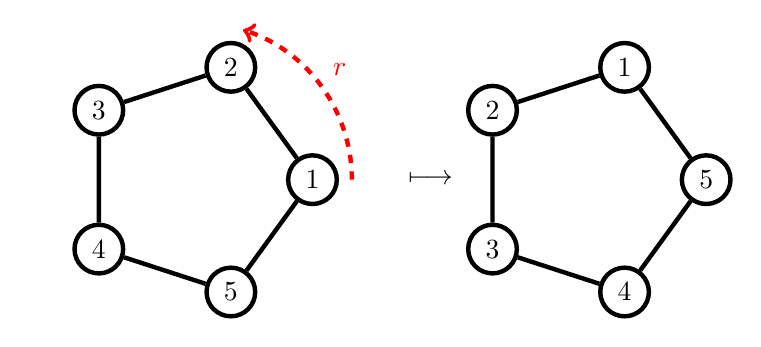
\begin{tikzpicture}
\node at (-2,0) {};
\draw[red, dashed, ultra thick, ->] (2,0)  arc(0:72:2) node[midway, above right] {$r$};
\path (1.5,0) node[circle, draw, ultra thick] (0) {1}
(72:1.5) node[circle, draw, ultra thick] (1) {2}
(144:1.5) node[circle, draw, ultra thick] (2) {3}
(216:1.5) node[circle, draw, ultra thick] (3) {4}
(288:1.5) node[circle, draw, ultra thick] (4) {5};
\draw[ultra thick] (0) -- (1) -- (2) -- (3) -- (4) -- (0);

\node at (3, 0) {$\bb \longmapsto$};

\begin{scope}[shift = {(5,0)}]

\path (1.5,0) node[circle, draw, ultra thick] (0) {5}
(72:1.5) node[circle, draw, ultra thick] (1) {1}
(144:1.5) node[circle, draw, ultra thick] (2) {2}
(216:1.5) node[circle, draw, ultra thick] (3) {3}
(288:1.5) node[circle, draw, ultra thick] (4) {4};
\draw[ultra thick] (0) -- (1) -- (2) -- (3) -- (4) -- (0);
\end{scope}
\end{tikzpicture}
\end{center}
\begin{center}
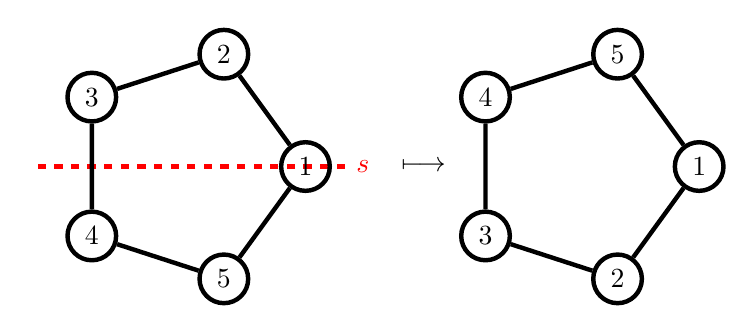
\begin{tikzpicture}
\draw[red, dashed, ultra thick] (2,0)  node[right] {$s$} -- (-2,0);
\path (1.5,0) node[circle, draw, ultra thick] (0) {1}
(72:1.5) node[circle, draw, ultra thick] (1) {2}
(144:1.5) node[circle, draw, ultra thick] (2) {3}
(216:1.5) node[circle, draw, ultra thick] (3) {4}
(288:1.5) node[circle, draw, ultra thick] (4) {5};
\draw[ultra thick] (0) -- (1) -- (2) -- (3) -- (4) -- (0);

\node at (3, 0) {$\bb \longmapsto$};

\begin{scope}[shift = {(5,0)}]

\path (1.5,0) node[circle, draw, ultra thick] (0) {1}
(72:1.5) node[circle, draw, ultra thick] (1) {5}
(144:1.5) node[circle, draw, ultra thick] (2) {4}
(216:1.5) node[circle, draw, ultra thick] (3) {3}
(288:1.5) node[circle, draw, ultra thick] (4) {2};
\draw[ultra thick] (0) -- (1) -- (2) -- (3) -- (4) -- (0);
\end{scope}
\end{tikzpicture}
\end{center}
\end{multicols}

\begin{Lem}\label{normal} Let $D_n$ be the dihedral group with $r$ and $s$ defined as above. Then $sr^ks^{-1} = r^{-k}$. In particular, $sr^k = r^{-k}s$.
\end{Lem}
\begin{pf}
Consider the symmetry $sr^ks^{-1}$. Since $s^2=1$, we have $s^{-1} =s$ and $sr^ks^{-1} = sr^ks$. In terms of the geometry transformations, $sr^ks$ means to reflect across the real axis, rotation $\theta=\dfrac{2\pi k}{n}$ counterclockwise, and reflect back. The net effect to the polygon is then just rotation $\theta = \dfrac{2\pi k}{n}$ clockwise, which is exactly $(r^{-1})^k = r^{-k}$. This establishes $sr^ks^{-1} = r^{-k}$. Multiplying both sides on the right by $s$ then gives $sr^k = r^{-k}s$.
\end{pf}\vs

\begin{Thm} The group $D_n$ is generated by the symmetries $r$ and $s$ defined above. In particular, every symmetry $\sigma$ can be expressed in the form $\sigma = r^ks^\ell$ for $k, \ell \in \Z$. 
\end{Thm}
\begin{pf}
From geometry, the only symmetries of the unit circle are rotations and reflections. These are the only types of symmetries for the regular $n$-gon which is a subset of the unit circle. All counterclockwise rotational symmetries of the $n$-gon are powers of $r$. All clockwise rotational symmetries of the $n$-gon are powers of $r^{-1}$. Let $\rho$ be a reflection across the line $\mathcal{L}$. If $\rho$ is a symmetry of the $n$-gon, then $\mathcal{L}$ must pass through the origin and we can measure and represent $\mathcal{L}$ by the angle $\theta$ it makes with the positive real axis. In order to be a symmetry, $\mathcal{L}$ must pass through a vertex or the midpoint of an edge of the polygon. In either case, $\theta = k\left(\dfrac{\pi}{n}\right)$. Let $r_\theta$ be the rotation counterclockwise by $\theta$. The $\rho = r_\theta s r_\theta^{-1}$. Then \lemref{normal} shows that $\rho = r_\theta r_\theta s = r_{2\theta}s = r^ks$. Therefore, every symmetry is generated by $r$ and $s$.\\

Each product of $r$'s and $s$'s is called a \textbf{word}. We can simplify words by collapsing down adjacent $r$'s together and adjacent $s$'s together. Since $s^2=1$, a generic word in $D_n$ looks like \[\sigma = r^{k_0}sr^{k_1}sr^{k_2}\cdots sr^{k_m},\] where $k_0$ and $k_m$ may be zero. We will induct on the number of $s$'s in $\sigma$. For our base case, suppose that $s$ appears zero times. Then $\sigma=r^{k_0} = r^{k_0}s^0$. For our inductive hypothesis, suppose that if $\sigma$ involves $m-1$ many $s$'s, then it can be expressed as $\sigma = r^ks^\ell$. Suppose that \[\sigma = r^{k_0}sr^{k_1}sr^{k_2}\cdots sr^{k_m}.\] Then $\sigma = \rho s r^{k_m}$ for some permutation $\rho$ which can be expressed with $m-1$ many $s$'s. By our inductive hypothesis, we get 
\[\sigma = \rho sr^{k_m} = (r^ks^\ell)sr^{k_m} = r^ks^{\ell+1}r^{k_m}= r^kr^{(-1)^{\ell+1}k_m}s^{\ell+1},\] where the last equality comes from \lemref{normal}. Therefore, the result follows by induction.
\end{pf}\vs

We call the expression $\sigma = r^ks^\ell$ the \textbf{normal form} of $\sigma$, which is unique up to modulo $n$ on $k$ and modulo 2 on $\ell$.

\begin{Cor} The order of $D_n$ is $2n$.\end{Cor}
\begin{pf} Since each symmetry in $D_n$ can be expressed in the normal form $r^ks^\ell$ for some $k, \ell\in \Z$, we count the possible normal forms in $D_n$. Since $r^n=1$ and $s^2=1$, there exists $n$ choices for $k$ and $2$ choices for $\ell$. This gives $|D_n| = 2n$.
\end{pf}\vs

\begin{Exam} Labeling the vertices of triangle clockwise as $1, 2, 3$ (or $1, e^{4/3\pi i}, e^{2/3\pi i}$), we get the 6 symmetries of the triangle:
\[\begin{alignedat}{100}
&1\  &\quad& r = (123)\ &\quad& r^2 = (132)\\
&s = (23)\ &\quad& rs = (12)\ &\quad& r^2s = (13)
\end{alignedat}\]

Similarly, if we label the vertices of the square clockwise as $1, 2, 3, 4$, we get the 8 symmetries of the square:
\[\begin{alignedat}{100}
&1\  &\quad& r = (1234)\ &\quad& r^2 = (13)(24)\ &\quad& r^3 = (1432)\\
&s = (24)\ &\quad& rs = (12)(34)\ &\quad& r^2s = (13)\ &\quad& r^3s = (14)(23)
\end{alignedat}\]
\end{Exam}\vs

Symmetry groups can also be discussed for three-dimensional objects. For example, the groups of symmetries of the tetrahedron and cube are $A_4$ and $S_4$, respectively. For the tetrahedron, each symmetry permutes the four vertices, so naturally this permutation group is a subgroup of $S_4$. As for the cube, symmetries of the cube necessarily permute the four interior diagonals of the cube, thus giving a permutation group in $S_4$.\\

%Solution 12.4: a) Z_1, b) D_4, c) D_3=S_3

\vfill
\stepcounter{footnote}\footnotetext{See \href{http://abstract.ups.edu/aata/permute-section-dihedral-groups.html}{\S 5.2 Dihedral Groups
} in Judson's \href{https://judsonbooks.org/aata/}{Abstract Algebra: Theory and Applications} for additional reading.}
\pagebreak

\startExercises{dihedral}

\begin{enumerate}[!HW!]
\item Write element in $D_5$ in cycle notation and in normal form.  %\emph{\color{magenta} $r=(12345),  s=(25)(34)$}
\item Prove that $D_n$ is nonabelian for $n\ge 3$.
\item Recall that the \hyperref[def:center]{\textbf{center}} of a group is $Z(G) = \{z\in G\mid \forall g\in G, gz=zg\}$. Find $Z(D_8)$, $Z(D_{10})$, and $Z(D_{2n})$. 
\end{enumerate}

\begin{Def} We say that a \textbf{rigid motion} if a function $f:\R^n\to \R^n$, for $n\in \N$, if $\Vert f(\bb x)-f(\bb y)\Vert = \Vert\bb x-\bb y\Vert$ for all $\bb x, \bb y\in \R^n$, that is, $f$ preserves the distance between vectors in the domain and vectors in the image. Let $X\subseteq \R^n$. Then \textbf{the symmetry group} of $X$ is the set of rigid motions $f : \R^n\to \R^n$ for which $f(X)=X$.
\end{Def}\vs

In other words, a symmetry is a rigid motion that moves the shape back onto itself. Note that if we view the regular $n$-gon as a subset of $\R^2$, then $D_n$ is the symmetry group of the regular $n$-gon. \\

For Exercises \ref{exer:symmetrygroupfirst:start}--\ref{exer:symmetrygroupfirst:stop}, determine the symmetry group of the given subset of $\R^2$. Note that symmetries of colored shapes  must preserve the coloring.
\begin{enumerate}[!HW!]
\begin{multicols}{3}
\item\label{exer:symmetrygroupfirst:start} \mbox{}\vspace{-15pt}

\begin{center}
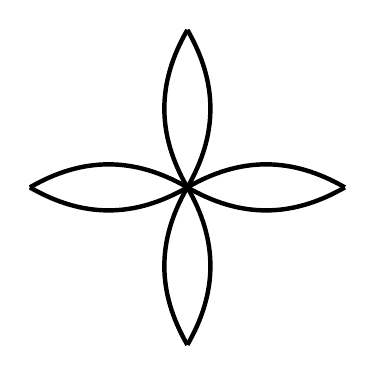
\begin{tikzpicture}
\draw[ultra thick] (-1,1) edge[bend left] (1,1) (1,3) edge[bend left] (1,1) (3,1) edge[bend left] (1,1) (1,-1) edge[bend left] (1,1)
(-1,1) edge[bend right] (1,1) (1,3) edge[bend right] (1,1) (3,1) edge[bend right] (1,1) (1,-1) edge[bend right] (1,1);
\end{tikzpicture}
\end{center} %$D_4$

\item  \mbox{}\vspace{-15pt}

\begin{center}
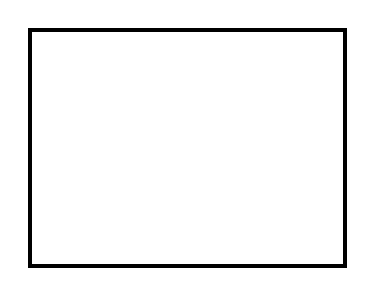
\begin{tikzpicture}
\draw[ultra thick] (0,0) rectangle (4,3);
\end{tikzpicture}
\end{center}\columnbreak %$V_4$

\item  \mbox{}\vspace{-15pt}

\begin{center}
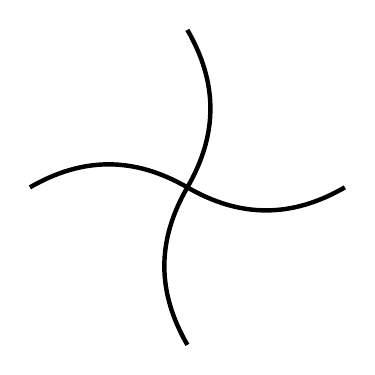
\begin{tikzpicture}
\draw[ultra thick] (-1,1) edge[bend left] (1,1) (1,3) edge[bend left] (1,1) (1,-1) edge[bend left] (1,1) (3,1) edge[bend left] (1,1);
\end{tikzpicture}
\end{center} %$Z_4$
\end{multicols}
\begin{multicols}{3}
\item  \mbox{}\vspace{-15pt}

\begin{center}
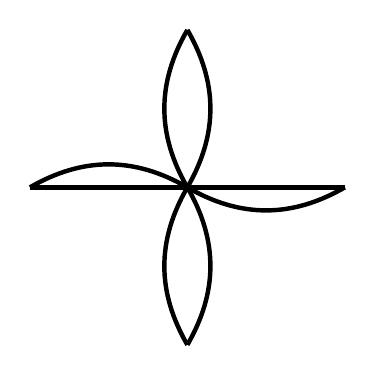
\begin{tikzpicture}
\draw[white] (-0.5,2.5) -- (2.5,2.5);
\draw[ultra thick] (-1,1) edge[bend left] (1,1) (1,3) edge[bend left] (1,1) (3,1) edge[bend left] (1,1) (1,-1) edge[bend left] (1,1)
(-1,1) edge (1,1) (1,3) edge[bend right] (1,1) (3,1) edge (1,1) (1,-1) edge[bend right] (1,1);
\end{tikzpicture}
\end{center} %$Z_2$

\item  \mbox{}\vspace{-15pt}

\begin{center}
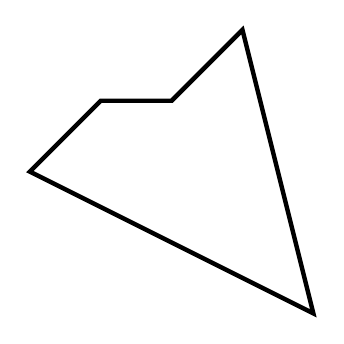
\begin{tikzpicture}[scale=0.9]
\draw[ultra thick] (0,0) -- (1,1) -- (2,-3) -- (-2,-1) --  (-1,0) -- cycle;
\end{tikzpicture}
\end{center}\columnbreak%Z_1

%\item  \mbox{}\vspace{-15pt}
%
%\begin{center}
%\begin{tikzpicture}
%\draw[ultra thick] (0,0) circle (2);
%\end{tikzpicture}
%\end{center} %S^1
%\end{multicols}
%\begin{multicols}{3}
\item  \mbox{}\vspace{-15pt}

\begin{center}

\begin{tikzpicture}
\filldraw[ultra thick, fill = cyan] (0.25, 0.25) -- (1,0) --  (0.25, -0.25) --  (0, -1) --  (-0.25, -0.25) -- (-1,0) --  (-0.25, 0.25) -- (0,1) -- cycle;
\end{tikzpicture}
\end{center} %$D_4$
\end{multicols}
\begin{multicols}{3}

\item  \mbox{}\vspace{-15pt}

\begin{center}

\begin{tikzpicture}
\filldraw[ultra thick, fill = cyan] (0.25, 0.25) -- (1,0) --  (0.25, -0.25) --  (0, -1) --  (-0.25, -0.25) -- (-1,0) --  (-0.25, 0.25) -- (0,1) -- cycle;
\filldraw[ultra thick, fill=magenta] (0.5, 1.1) -- (0,0.5) -- (-0.5, 1.1) -- cycle
(0.5, -1.1) -- (0,-0.5) -- (-0.5, -1.1) -- cycle
(1.1, 0.5) -- (0.5, 0) -- (1.1, -0.5) -- cycle
(-1.1, 0.5) -- (-0.5, 0) -- (-1.1, -0.5) -- cycle;
\filldraw[ultra thick, fill=yellow] (0,0) circle (0.1);
\end{tikzpicture}
\end{center}  %$D_4$

\item \mbox{}\vspace{-15pt}

\begin{center}
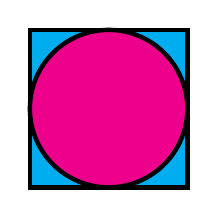
\begin{tikzpicture}
\filldraw[ultra thick, fill = cyan] (-1,-1) rectangle (1,1);
\filldraw[ultra thick, fill=magenta] (0,0) circle (1.);
\end{tikzpicture}
\end{center}  %$D_4$
%\end{multicols}
%\begin{multicols}{3}
\item\label{exer:symmetrygroupfirst:stop}  \mbox{}\vspace{-15pt}

\begin{center}
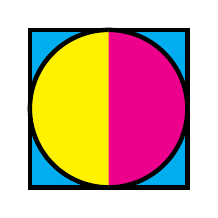
\begin{tikzpicture}
\filldraw[ultra thick, fill = cyan] (-1,-1) rectangle (1,1);
\filldraw[ultra thick, fill=magenta] (0,0) circle (1.);
\begin{scope}
\clip (0, -1) rectangle (-1,1);
\filldraw[ultra thick, fill=yellow] (0,0) circle (1.);
\end{scope}
\end{tikzpicture}
\end{center} %$Z_2$
%
%\columnbreak \mbox{}
%
%\columnbreak \mbox{}
\end{multicols}
\end{enumerate}

\vfill
\pagebreak

%%%%%%%%%%%% Supplementary Exercises %%%%%%%%%%%%%%%%%%%%%%%%%%%%%%%%%%%%%%%%%%%%%%%%%%%%%%%%%%
%%%%%%%%%%%%%%%%%%%%%%%%%%%%%%%%%%%%%%%%%%%%%%%%%%%%%%%%%%%%%%%%%%%%%%%%%%%%
\startSuppExercises{permutation}

\begin{enumerate}[!HW!]
\item Find $(a_1a_2\ldots a_n)^{-1}$. 
\item List all of the subgroups of $S_4$.\\

For Exercises \ref{exer:permsuppS4:start}--\ref{exer:permsuppS4:stop}, compute the given subset of $S_4$. Is it a subgroup?
\begin{multicols}{3}
\item \label{exer:permsuppS4:start} $\{\sigma\in S_4\mid \sigma(1)=3\}$ 
\item $\{\sigma\in S_4\mid \sigma(2)=2\}$ 
\item\label{exer:permsuppS4:stop} $\{\sigma\in S_4\mid \sigma(1)=3, \sigma(2)=2\}$
\end{multicols}\vs

\item  Find an element of largest order in $S_n$ for $n=3, \ldots, 10$.
\item Let $\sigma \in S_n$ have order $n$. Show that for all integers $i$ and $j$, $\sigma^i=\sigma^j$ if and only if $i\equiv j\pmod n$.
\item\label{exer:snnonabelian} Prove that $S_n$ is nonabelian for $n\ge 3$. 
\item If $\sigma\in S_n$ is not a cycle,  then $\sigma$ can be written as the product of at most $n-2$ transpositions.
\item If $\sigma\in S_n$ can be expressed as an odd number of transpositions, show that any other product of transpositions equaling $\sigma$ must also be odd.
\item Show that $\alpha^{-1}\beta^{-1}\alpha\beta\in A_n$ for all $\alpha,\beta\in S_n$.

\item Show that, in $D_n$, $srs=r^{-1}$.
\item Show that, in $D_n$, $r^ks=sr^{-k}$ for all $k\in \Z$.
\item Show that, in $D_n$, $|r^k| = \dfrac{n}{\gcd(k,n)}$ for all $k\in \Z$.

\item Show that the symmetry group of the tetrahedron is $A_4$.
\item\label{exer:symmetrycube} Show that the symmetry group of the cube is $S_4$.

\item For $\alpha,\beta\in S_n$, define $\alpha\sim\beta$ if there exists some $\sigma\in S_n$ such that $\sigma\alpha\sigma^{-1}=\beta$. Show that $\sim$ is an equivalence relation on $S_n$. We say that $\alpha$ and $\beta$ are \textbf{conjugates} if $\alpha\sim \beta$.
\item Show that $\alpha,\beta\in S_n$ have the same cycle structure if and only if $\alpha$ and $\beta$ are conjugates.\\

For Exercises \ref{exer:symmetricequiv:start}--\ref{exer:symmetricequiv:stop}, for a fixed permutation $\sigma\in S_X$, define a relation $\sigma$ on $X$ by the rule $x\sim_\sigma y$ if and only if there exists a $n\in \Z$ such that $\sigma^n(x)=y$, for $x,y\in X$.
\item\label{exer:symmetricequiv:start} Prove that $\sim_\sigma$ is an equivalence relation.
\item Compute the equivalence classes of $\sim_\sigma$ for each element of $X=\{1,2,3,4,5\}$ is $\sigma = (1254)$.
\item Compute the equivalence classes of $\sim_\sigma$ for each element of $X=\{1,2,3,4,5\}$ is $\sigma = (123)(45)$.
\item Compute the equivalence classes of $\sim_\sigma$ for each element of $X=\{1,2,3,4,5\}$ is $\sigma = (13)(25)$.

\begin{Def} Let $H\le S_X$. We say that $H$ is \textbf{transitive} if for all $x,y\in X$ there exists $\sigma\in H$ such that $\sigma(x)=y$.
\end{Def}\vs
\item\label{exer:symmetricequiv:stop}  Prove that $H$ is transitive if and only  if $\sim_\sigma$ has a single equivalence class for each $\sigma\in H$.
\end{enumerate}


\pagebreak

%%%%%%%%%%%% CHAPTER 5 %%%%%%%%%%%%%%%%%%%%
%%%%%%%%%%%%%%%%%%%%%%%%%%%%%%%%%%%%%%%%%%%%%%%%%%%%%%%%%%%%%%%%%%%%%%%%%%%%%%%%
\chapterlabel{Cosets}{cosets}\pagebreak

%%%%%%%%%%%% Section 5.1 %%%%%%%%%%%%%%%%%%%%%%%%%%%%%%%%%%%%%%%%%%%%%%%%%%%%%%%%%%
%%%%%%%%%%%%%%%%%%%%%%%%%%%%%%%%%%%%%%%%%%%%%%%%%%%%%%%%%%%%%%%%%%%%%%%%%%%%
\begin{center} 
\emph{``War does not determine who is right -- only who is left.'' --  Bertrand Russell}
\end{center}

\begin{Videos}
\video{https://youtu.be/gYoRD5z47EA}{Cosets} &
\video{https://youtu.be/9o4zK7dMQFs}{Cosets Partition a Group} &
\video{https://youtu.be/y5kMfc9ZgnI}{Counting Cosets}
\end{Videos}

\sectionlabel{Cosets}{cosets}
\begin{Def} Let $G$ be a group and let $H\le G$. Define a \textbf{left coset} of $H$ with representative $g\in G$ to be the set
\[gH = \{gh\mid h\in H\}.\] Let $G/H$ denote the set of left cosets of $G$ with respect to $H$.\\


Similarly, we define the \textbf{right coset} as
\[Hg = \{hg\mid h\in H\}.\] Let $H\backslash G$ denote the set of right cosets of $G$ with respect to $H$.
\end{Def}\vs

It should be mentioned that although cosets are subsets of $G$ constructed from a subgroup $H$ of $G$, the cosets $gH$ and $Hg$ are not necessarily subgroups themselves, nor are they necessarily equal.

\begin{Exam} Let $H = \langle 3\rangle \le \Z_6$, that is, $H = \{0, 3\}$. There are then three left cosets:
\[\begin{alignedat}{100}
0+H\ &=\ &3+H\ &=\ & \{0, 3\}\\
1+H\ &=\ &4+H\ &=\ & \{1, 4\}\\
2+H\ &=\ &5+H\ &=\ & \{2, 5\}\\
\end{alignedat}\] Because $\Z_6$ is an additive group, the cosets are written with additive notation as well. When the identity is used to represent a coset, such as $0+H$, it will be more convenient to suppress the identity and express the coset as just $H$. After all, $0+H = H$. Because $Z_6$ is abelian, the right cosets are the same as the left cosets.
\end{Exam}\vs

\begin{Exam} Let $H= A_3= \langle (123)\rangle \le S_3$, that is, $H= \{1, (123), (132)\}$. There are two distinct left cosets of $H$:
\[\begin{alignedat}{100}
H\ &=\ &(123)H\ &=\ & (132)H\ &=\ &\{1, (123), (132)\}\\
(12)H\ &=\ &(13)H\ &=\ & (23)H\ &=\ &\{(12), (13), (23)\}\\
\end{alignedat}\] Interesting enough, one coset is the set of even permutations ($A_3$) and the other is the set of odd permutations ($B_3$). Even though $S_3$ is nonabelian, it is still the case that the right cosets coincide with the left cosets:
\[\begin{alignedat}{100}
H\ &=\ &H(123)\ &=\ & H(132)\ &=\ &\{1, (123), (132)\}\\
H(12)\ &=\ &H(13)\ &=\ & H(23)\ &=\ &\{(12), (13), (23)\}\\
\end{alignedat}\]

Before we begin to believe this is always that case, let $K = \langle (12)\rangle = \{1, (12)\}$. Then the left and right cosets are listed below:\vspace{-0.25 in}
\begin{multicols}{2}
\[\begin{alignedat}{100}
K\ &=\ &(12)K\ &=\ \{1, (12)\}\\
(123)K\ &=\ &(13)K\ &=\ \{(123), (13)\}\\
(132)K\ &=\ &(23)K\ &=\ \{(132), (23)\}\\
\end{alignedat}\]


\[\begin{alignedat}{100}
K\ &=\ &K(12)\ &=\ \{1, (12)\}\\
K(123)\ &=\ &K(23)\ &=\ \{(123), (23)\}\\
K(132)\ &=\ &K(13)\ &=\ \{(132), (13)\}\\
\end{alignedat}\] 
\end{multicols}Thus, it is possible that $gK\neq Kg$. This is actually a very frequent occurrence in nonabelian groups. 
\end{Exam}\vs


\begin{Thm} Let $H\le G$. We define a relation on $G$ by the rule $x\sim y$ if and only if $x^{-1}y \in H$. Then this is an equivalence relation where the equivalence classes are the left cosets $gH$. In particular, the left cosets form a partition on the group $G$.
\end{Thm}
\begin{pf}
Let $x\in G$. Then $x^{-1}x = e \in H$, since $H$ is a subgroup of $G$. Thus, $x\sim x$ and $\sim$ is reflexive. Next, let $x\sim y$ for some $x, y\in G$. Then $x^{-1}y\in H$. Since $H$ is a subgroup, $y^{-1}x = (x^{-1}y)^{-1}\in H$. Thus, $y\sim x$ and $\sim$ is symmetric. Finally, let $x\sim y$ and $y\sim z$ for some $x,y,z\in H$. Then $x^{-1}y, y^{-1}z\in H$. Since $H$ is a subgroup, $x^{-1}z = (x^{-1}y)(y^{-1}z)\in H$. Thus, $x\sim z$ and $\sim$ is transitive. Therefore, $\sim$ is an equivalence relation on $G$.\\

We next will show that $[g] = gH$. Let $x\in gH$. Then there exists some $h\in H$ such that $x=gh$. Then $g^{-1}x = g^{-1}(gh) = h\in H$, which shows that $x\in [g]$. Thus, $gH\subseteq [g]$. The containment $[g]\subseteq gH$ is handled similarly. Therefore, $[g]=gH$, that is, the left cosets are the equivalence classes of the relation $\sim$.
\end{pf}\vs

An analogous statement about right cosets can be made, with similar proof, using the relation $x\sim y$ if and only if $xy^{-1}\in H$.

\begin{Thm} Let $G$ be a group with $H\le G$ and $g\in G$. Then $|H| = |gH|$.
\end{Thm}
\begin{pf}
We define a mapping $\varphi : H \to gH$ by the rule $\varphi(h) = gh$ for all $h\in H$, which is clearly well-defined. We claim that this mapping is bijective. For injectivity, let $\varphi(h) = \varphi(h')$ for $h,h'\in H$. Then $gh=gh'$. Cancelling $g$ on the left, we get $h=h'$. Thus, $\varphi$ is injective. For surjectivity, let $x\in gH$. Then there exists some $h\in H$ such that $x=gh$. So, $\varphi(h) = gh=x$. Thus, $\varphi$ is surjective, proving the claim. Since $\varphi$ is bijective, we conclude that $|H|=|gH|$. 
\end{pf}\vs

In particular, all left cosets have the same cardinality as $H$ and have the same cardinality as each other. A similar proof extends the analogous statement for right cosets.\\

\begin{Thm}\label{thm:samenumberofcosets} Let $H$ be a subgroup of a group $G$. Then $|G/H| = |H\backslash G|$.\end{Thm}
\begin{pf}
Like the previous proof, it suffices to construct a bijection between the two sets. Let $\varphi : G/H \to H\backslash G$ be defined by the rule $\varphi(gH) = Hg^{-1}$. Now, we need to check that this definition of $\varphi$ is well-defined since it is defined by a representative of $gH$, that is, we need to check that different representatives of $gH$ give the same image. Suppose that $aH = bH$. We claim that $Ha^{-1} = Hb^{-1}$. Let $x\in Ha^{-1}$. So there exists some $h\in H$ such that $x= ha^{-1}$. Then $x^{-1} = (ha^{-1})^{-1} = ah^{-1} \in aH$. Since $aH=bH$, this implies that there is some $k\in H$ such that $x^{-1} = bk$. Then $x = (bk)^{-1} = k^{-1}b^{-1}\in Hb^{-1}$. Therefore, $Ha^{-1} \subseteq Hb^{-1}$. The containment $Hb^{-1} \subseteq Ha^{-1}$ is handled similarly. Since we have established $Ha^{-1} = Hb^{-1}$ if $aH=bH$, we have proven that $\varphi$ is well-defined.\\

Define $\psi : H\backslash G \to G/H$ by the rule $\psi(Hg) = g^{-1}H$. By similarly reasoning, this mapping is also well-defined and is the inverse of $\varphi$. Since $\varphi$ is invertible, we conclude that $\varphi$ is bijective.
\end{pf}\vs

\begin{Prop} Let $H$ be a subgroup of a group $G$ and let $x,y\in G$. Then $xH = yH$ if and only if $y \in xH$.
\end{Prop}\vs

The proof is left as an exercise. As usual, as there is nothing particularly special about left cosets, the analogous result holds for right cosets also.

\vfill
\stepcounter{footnote}\footnotetext{See \href{http://abstract.ups.edu/aata/cosets-section-cosets.html}{\S 6.1 Cosets} in Judson's \href{https://judsonbooks.org/aata/}{Abstract Algebra: Theory and Applications} for additional reading.}
\pagebreak

\startExercises{cosets}

For Exercises \ref{exer:cosetcompute:start}--\ref{exer:cosetcompute:stop}, list all the left and right cosets of the given subgroup inside the given group.
\begin{enumerate}[!HW!]
\begin{multicols}{4}
\item\label{exer:cosetcompute:start} $\langle 8\rangle \le \Z_{24}$ 
\item $\langle 3\rangle \le \Z_{8}^*$ 
\item $3\Z\le \Z$ 
\item $A_4\le S_4$ 
\end{multicols}
\begin{multicols}{4}
\item $A_n\le S_n$ 
\item $D_4\le S_4$ 
\item $S^1\le \C^*$ 
\item\label{exer:cosetcompute:stop} $\langle (123)\rangle \le S_4$ 
\end{multicols}
\end{enumerate}

\begin{enumerate}[!HW!]
\item In the proof of \thmref{thm:samenumberofcosets}, we defined a function $\varphi : G/H \to H\backslash G$ be defined by the rule $\varphi(gH) = Hg^{-1}$. We then argued this is a well-defined bijection. Why could we not use instead $\varphi(gH) = Hg$? 
\end{enumerate}\vs

For Exercises \ref{exer:cosetproof:start}--\ref{exer:cosetproof:stop}, prove the given statement about cosets.
\begin{enumerate}[!HW!]
\item\label{exer:cosetproof:start} Let $H\le G$ and suppose $g\in G$ such that $ghg^{-1}\in H$ for all $h\in H$. Then $gH=Hg$. 

\item Let $H,K\le G$. Then, for any $g\in G$, $gH\cap gK$ is a left coset of $H\cap K$ inside of $G$. 

\item \label{exer:cosetproof:stop} Let $H\le G$ and $x,y\in G$. The following are equivalent:
\begin{enumerate}
\begin{multicols}{3}
\item $xH=yH$
\item $Hx^{-1}=Hy^{-1}$
\item $xH\subseteq yH$
\end{multicols}
\begin{multicols}{3}
\item $y\in xH$
\item $x^{-1}y\in H$
\end{multicols}
\end{enumerate}
\end{enumerate}\vs


\vfill
\pagebreak

%%%%%%%%%%%% Section 5.2 %%%%%%%%%%%%%%%%%%%%%%%%%%%%%%%%%%%%%%%%%%%%%%%%%%%%%%%%%%
%%%%%%%%%%%%%%%%%%%%%%%%%%%%%%%%%%%%%%%%%%%%%%%%%%%%%%%%%%%%%%%%%%%%%%%%%%%%
\begin{center} 
\emph{``Think left and think right and think low and think high. Oh, the thinks you can think up if only you try!'' -- Dr. Seuss}
\end{center}

\begin{Videos}
\video{https://youtu.be/M9pnBMGxKmQ}{The Index of a Subgroup} &
\video{https://youtu.be/yDvLibGs_q8}{Lagrange's Theorem} &
\video{https://youtu.be/VoM_FfWGVU0}{Euler's Theorem and Fermat's Little Theorem}
\end{Videos}

\sectionlabel{Lagrange's Theorem}{lagrange}
\begin{Def} Let $G$ be a group with subgroup $H$. Then we define the \textbf{index} of $H$ in $G$, denoted $[G:H]$, as the number of left cosets of $H$ in $G$, that is, $[G: H] = |G/H|$.
\end{Def}\vs

Since $|G/H| = |H\backslash G|$, we could equally have defined the index as the number of right cosets.

\begin{Exam} Let $G=\Z_6$ and $H = \langle 3\rangle = \{0, 3\}$. Then $[G:H] =3$ since there were three (left) cosets $H$, $1+H$, and $2+H$.\end{Exam}\vs

\begin{Exam} Let $G=S_3$, $H=A_3 = \{1, (123), (132)\}$, and $K = \{1, (12)\}$. Then $[G:H] = 2$, since $H$ has two left cosets: $H$ and $(12)H$, and $[G:K] = 3$, since $K$ has three left cosets $K$, $(123)K$, and $(132)K$.
\end{Exam}\vs

\begin{Thm}[Lagrange's Theorem] Let $G$ be a finite group and let $H\le G$. Then $[G:H] = |G|/|H|$. In particular, the order of $H$ divides the order of $G$.
\end{Thm}
\begin{pf}
Since $G$ is partitioned by the left cosets of $G$, two cosets are either equal or disjoint. In particular, $G$ is the disjoint union of all the distinct cosets of $H$. So, $|G|$ is the sum of each distinct coset's cardinality, which is always just $|H|$. As there are $[G:H]$ many cosets, we get $|G| = [G:H]\cdot |H|$, which proves the result.
\end{pf}\vs

\begin{Cor}\label{lagrange1} Suppose that $G$ is a finite group and $g\in G$. Then $|g|$ must divide $|G|$. In particular, $g^{|G|} =e$.
\end{Cor}
\begin{pf} Let $|G| = n$ and $|g| = m$. The cyclic subgroup $\langle g\rangle$ is clearly a subgroup of $G$ and $|\langle g\rangle | = m$. By Lagrange's Theorem, $m\mid n$, that is, there exists some $k\in \Z$ such that $km=n$. Then $g^{n} = g^{km} = (g^m)^k = e^k = e$.
\end{pf}\vs

\begin{Cor} Let $|G| = p$ a prime. Then $G$ is cyclic and any $g\in G$ such that $g\neq e$ is a generator of $G$. \end{Cor}
\begin{pf} Let $g\in G$. Let $|g| = n$. By Lagrange's Theorem, $n\mid p$, but since $p$ is prime either $n=1$ or $n=p$. If $n=1$, then $g=e$. If $n=p=|G|$, then $\langle g\rangle = G$.
\end{pf}\vs

\begin{Cor} Let $H$ and $K$ be subgroups of a finite group $G$ such that $K\subseteq H\subseteq G$. Then 
\[[G:K] = [G:H][H:K].\]
\end{Cor}
\begin{pf} Note that 
\[[G:K] = \dfrac{|G|}{|K|} = \dfrac{|G|}{|K|}\left(\dfrac{|H|}{|H|}\right) = \dfrac{|G|}{|H|}\left(\dfrac{|H|}{|K|}\right) = [G:H][H:K]. \qedhere\]
\end{pf}\vs

The previous result is also true for infinite groups with subgroups of finite index but much more involved to prove.\\

It is important to recognize that the converse of Lagrange's Theorem is not true in general, that is, if $d\mid |G|$ then there is not necessarily a subgroup of order $d$. For example, $|A_4| = 24$ and $6\mid 24$ but $A_4$ has no subgroup of order 6. To see this, assume to the contrary that $H\le A_4$ and $|H|=6$. Clearly, $1\in H$. There are only three 2-2 cycles in $A_4$. Thus, $H$ must contain a 3-cycle and its inverse. As these come in inverse pairs, $H$ must also contain a 2-2 cycle. But any 3-cycle and 2-2-cycle generate all of $A_4$ together, which can be proven. Therefore, $A_4$ has no subgroup of order 6.\\

The \textbf{Euler $\phi$-function}, also called the \textbf{totient function}, is a map $\phi : \Z^+ \to \R$ such that $\phi(1) = 1$ and $\phi(n)$ is equal to the number of positive integers coprime to $n$ for $n>1$. In particular, we have shown that $|\Z_n^*| = \phi(n)$. The following two important theorems from number theory are more corollaries of Lagrange's Theorem.

\begin{Thm}[Euler's Theorem] Let $a$ and $n$ be integers such that $n>0$ and $\gcd(a,n)=1$. Then \[a^{\phi(n)} \equiv 1 \pmod n.\]\end{Thm}
\begin{pf}
The result follows from \corref{lagrange1} since $a\in \Z_n^*$ and $|\Z_n^*| = \phi(n)$. 
\end{pf}\vs

\begin{Thm}[Fermat's Little Theorem] Let $p$ be prime. If $p \nmid a$, then 
\[a^{p-1} \equiv 1 \pmod p.\] Furthermore, $b^p \equiv b \pmod p$ for any integer $b$.
\end{Thm}
\begin{pf} Since $\phi(p) = p-1$, the first equation follows immediately from Euler's Theorem. As for the second equation, if $p \nmid b$, then $b^{p-1} \equiv 1 \pmod p$. Multiplying both sides by $b$ then gives the identity. If $p\mid b$, then $b\equiv 0 \pmod p$ and $b^p \equiv 0^p \equiv 0 \equiv b\pmod p$.
\end{pf}\vs

Fermat's Little Theorem leads to a very basic primality test in number theory as illustrated in \examref{exam:primalitytest}. If we are uncertain if $n$ is prime, we can choose some positive integer $a<n$. We first can compute $d=\gcd(a,n)$ (using the Euclidean algorithm). If $d\neq 1$, then $d\mid n$ and $n$ is not prime. If $d=1$, compute $a^{n-1} \pmod n$ (using the Repeated Squares algorithm). If this value is not congruent to $1$, then we can conclude that $n$ is not prime even though you do not necessarily know a factorization of $n$. If $a^{n-1} \equiv 1 \pmod n$) for a ``large'' list of integers $a$, then we can conclude that $n$ is probably prime. 

\vfill
\stepcounter{footnote}\footnotetext{See \href{http://abstract.ups.edu/aata/cosets-section-cosets.html}{\S 6.1 Cosets}, \href{http://abstract.ups.edu/aata/cosets-section-lagranges-theorem.html}{\S 6.2 Lagrange's Theorem}, and \href{http://abstract.ups.edu/aata/cosets-section-fermat-euler.html}{\S 6.3 Fermat's and Euler's Theorems} in Judson's \href{https://judsonbooks.org/aata/}{Abstract Algebra: Theory and Applications} for additional reading.}
\pagebreak

\startExercises{lagrange}

\begin{enumerate}[!HW!]
\item Suppose that $|G|=60$ is a group. What are the possible orders of subgroups of $G$?\\ %1, 2, 3, 4, 5, 6, 10, 12, 15, 20, 30, 60

For Exercises \ref{exer:lagrangeproof:start}--\ref{exer:lagrangeproof:stop}, prove the given statement about orders and indices.

\item\label{exer:lagrangeproof:start} Suppose that $G$ is a finite group with $g,h\in G$ such that $|g|=5$ and $|h|=7$. Then $|G|\ge 35$. %\emph{\color{magenta} $|g|, |h| \mid |G|$}

\item If $p=4n+3$ is prime, then there is no solution to $x^2\equiv -1\pmod p$. %\emph{\color{magenta} Use Fermat's Little Theorem.}

\item \label{exer:lagrangeproof:stop} As additive groups, $[\Q:\Z] =\infty$.
\end{enumerate}\vs


\begin{Exam}[Fermat's Little Primality Test]\label{exam:primalitytest} By Fermat's Little Theorem, if $p$ is prime and $p\nmid a$, then $a^{p-1}\equiv 1\pmod p$. Note that by this identity 15 cannot be a prime since
\[2^{15-1} \equiv 2^14 \equiv 4 \not\equiv 1 \pmod {15}.\] Note that we can observe that $15$ is composite without determining its factorization (of course, we know $15=3(5)$). Conversely, 
\[2^{17-1} \equiv 2^{16} \equiv 1\pmod{17},\] so by Fermat's Little Theorem, $17$ could be prime (which we know it is). 

\begin{Def} Let $n\in \Z$. We say that $n$ is a \textbf{pseudoprime} if $2^{n-1}\equiv 1\pmod n$ but  $n$ is composite.
\end{Def} 

Hence, pseudoprimes appear to be prime from Fermat's primality test but actuarlly are not. Hence, \emph{Fermat's Little Test} can determine whether a number is \emph{certainly composite} (such as 15) or \emph{maybe prime} (such as 17). It cannot, by itself, determine whether a number is prime but it can determine when a number is composite but provides no clue to its factorization. 
\end{Exam}\vs

For Exercises \ref{exer:pseudoprime:start}--\ref{exer:pseudoprime:stop}, for the given $n$, compute $2^{n-1}\pmod n$. Determine whether $n$ is certainly composite or maybe prime. \hyperref[exam:magma:modexp]{MAGMA is recommended for these exercises}.
\begin{enumerate}[!HW!]
\begin{multicols}{6}
\item \label{exer:pseudoprime:start} 342 
\item 811
\item 601 
\item 561 
\item 771 
\item\label{exer:pseudoprime:stop} 631 
\end{multicols}
\end{enumerate}

\begin{Exam} The primality test of \examref{exam:primalitytest} was conducted using $a=2$, but any base $a$ such that $\gcd(a,n)=1$ would work (note that if $d=\gcd(a,n)>1$, then we know that $n$ is composite since $d\mid n$).  Consider $n=341$. Note that 
\[2^{341-1} \equiv 2^{340} \equiv 1 \pmod{341},\] but \[3^{341-1} \equiv 3^{340} \equiv 56 \pmod{341}.\] So, while Fermat's Little Test using $a=2$ determined that $341$ is maybe prime, using $a=3$ gives that $341$ is composite. Thus, $341$ is a pseudoprime.

\begin{Def} Let $n, a\in \Z$. We say that $n$ is a \textbf{pseudoprime base} $a$ if $\gcd(a,n)=1$ and $a^{n-1}\equiv 1\pmod n$ but  $n$ is composite.
\end{Def} 

Pseudoprimes of various bases do exist, but if $n$ is determined to be composite by some base $a$, regardless if it is pseudoprime for many other bases, then $n$ is not prime. Hence, Fermat's Little Test can be greatly improved by testing various bases $a$. If $n$ again and again is determined to be maybe prime for several different bases, then we can conclude that $n$ is probably prime. Unfortunately, this test, with several different bases, cannot determine whether $n$ is certianly prime because of \textbf{Carmichael numbers}, that is, numbers which are pseudoprime of base $a$ for all integers $a$ coprime to $n$. For example, $n=561$ is a Carmichael number. Clearly, $561=3(11)(17)$, but if you compute $a^{560} \pmod{561}$, then you always get $1$ if $3, 11, 17\nmid a$. Carmichael numbers with no small prime could trick this test, but fortunately Carmichael numbers are rare among the integers even though there are infinitely many of them.
\end{Exam}\vs

For Exercises \ref{exer:carmichael:start}--\ref{exer:carmichael:stop}, for the given $n$, compute $3^{n-1}\pmod n$. Comparing results from Exercises \ref{exer:pseudoprime:start}--\ref{exer:pseudoprime:stop}, determine whether $n$ is certainly composite or probably prime. \hyperref[exam:magma:modexp]{MAGMA is recommended for these exercises}.
\begin{enumerate}[!HW!]
\begin{multicols}{6}
\item \label{exer:carmichael:start} 342 
\item 811 
\item 601 
\item 561 
\item 771 
\item\label{exer:carmichael:stop} 631 
\end{multicols}
\end{enumerate}

\vfill
\pagebreak

%%%%%%%%%%%% Supplementary Exercises %%%%%%%%%%%%%%%%%%%%%%%%%%%%%%%%%%%%%%%%%%%%%%%%%%%%%%%%%%
%%%%%%%%%%%%%%%%%%%%%%%%%%%%%%%%%%%%%%%%%%%%%%%%%%%%%%%%%%%%%%%%%%%%%%%%%%%%
\startSuppExercises{cosets}

\begin{enumerate}[!HW!]
\item Describe the left cosets of $\SL_2(\R)\le \GL_2(\R)$. Compute $[\GL_2(\R):\SL_2(\R)]$.
\item\label{verify:Euler} Verify Euler's Theorem for $n=15$ and $a=4$. 

\item Suppose that $[G:H]=2$. If $a,b\in G\setminus H$, show that $ab\in H$.
\item Suppose that $[G:H]=2$. Show that $gH=Hg$ for all $g\in G$.

\item Let $G$ be  a cyclic group of order $n$. Show that there are $\phi(n)$ generators of $G$.
\item\label{exer:eulerfactor} Let $n=\prod_{i=1}^k p_i^{e_i}$, where $p_1,\ldots, p_k$ are distince primes. Prove that \[\phi(n) = n\prod_{i=1}^k\left(1-\dfrac{1}{p_i}\right).\] 
\item For all $n\in \Z^+$, prove $n=\dsum_{d\mid n}\phi(d)$.

\item For $H,K \le G$, define $a\sim b$ if there exists some $h\in H$ and $k\in K$ such that $hak=b$, for $a,b\in G$. Show that $\sim$ is an equivalence relation on $G$. The equivalence classes associated to $\sim$ are called \textbf{double cosets} relative to $H$ and $K$. Compute the double cosets $H=K=\langle (123)\rangle \le A_4$.\\

For Exercises \ref{exer:cosetdisprove:start}--\ref{exer:cosetdisprove:stop}, prove or disprove the given statement about cosets, orders, or indices.
\item\label{exer:cosetdisprove:start} If $g^n=e$, then $|g|\mid n$. 
\item Every subgroup of the integers has finite index. 
\item Every subgroup of the integers has finite order. 
\item\label{exer:cosetdisprove:stop} As additive groups, $[\C:\R] =\infty$. 
\end{enumerate}


\pagebreak

%%%%%%%%%%%% CHAPTER 6 %%%%%%%%%%%%%%%%%%%%
%%%%%%%%%%%%%%%%%%%%%%%%%%%%%%%%%%%%%%%%%%%%%%%%%%%%%%%%%%%%%%%%%%%%%%%%%%%%%%%%
\chapterlabel{Applied Algebra}{applied}\pagebreak
%%%%%%%%%%%% Section 6.1 %%%%%%%%%%%%%%%%%%%%%%%%%%%%%%%%%%%%%%%%%%%%%%%%%%%%%%%%%%
%%%%%%%%%%%%%%%%%%%%%%%%%%%%%%%%%%%%%%%%%%%%%%%%%%%%%%%%%%%%%%%%%%%%%%%%%%%%
\begin{center} 
\emph{``There are no secrets that time does not reveal.'' -- Jean Racine}
\end{center}

\begin{Videos}
\video{https://youtu.be/q-qx0Einjws}{Symmetric Key Cryptography} &
\video{https://youtu.be/87K4VFNGKGs}{Caesar Cipher} &
\video{https://youtu.be/JdSI8pT3O08}{Affine Cipher}
\end{Videos}

\sectionlabel{Symmetric Key Cryptography}{symmetrickey}
When people need to secretly store or communicate messages, they turn to cryptography. Cryptography involves using techniques to obscure a message so outsiders cannot read the message. It is typically split into two steps: encryption, in which the message is obscured, and decryption, in which the original message is recovered from the obscured form.

\begin{Def} A \textbf{cipher} replaces each letter (or number) in the message with a different letter, following some established mapping, called the \textbf{encryption mapping}. The pre-image of a message with respect to the encryption map is called the \textbf{plaintext}. The image of a message with respect to the encryption map is called the \textbf{ciphertext}. The mapping is necessarily bijective so ciphertexts can be converted back to the plaintext. This inverse mapping is called the \textbf{decryption mapping}.\\

 The strength of any cryptosystem depends on the difficulty of an eavesdropper (Eve) from discovery the decryption map. Although much (if not all) of the encryption mapping is public information, some information about the decryption mapping is kept secret, called the \textbf{key}, which without it the decryption mapping is too difficult to compute. \\

\textbf{Symmetric-Key Cryptography} is a method of cryptography where both the sender (Alice) and the receiver (Bob) use the same key for encryption and decryption.
\end{Def}\vs

The mappings commonly used in cryptography are algebraic and require the message to numerical. As such, we will use the simple rule $A = 0$, $B=1$, $C=2$, etc. to digitize a string of alphabetic characters as an array of numerical digits for cryptographic purposes.

\begin{Exam} Below is \href{https://github.com/emisseldine/Math4220/blob/main/Symmetric_Key_Cryptography}{MAGMA code}\footnotemark\ that can be used to implement the above encoding process. For simplicity, lower and upper case will be considered identical. Also, no numerical digits or special characters will be allowed. 

\begin{lstlisting}[language=Magma, firstnumber=3]
Digitize := function(message); 
E := [];
m := 0;
for i:= 1 to #message do
    case message[i]:
    when "a","A": E cat:=[0]; when "b","B": E cat:=[1]; when "c","C": E cat:=[2];
    when "d","D": E cat:=[3]; when "e","E": E cat:=[4]; when "f","F": E cat:=[5];
    when "g","G": E cat:=[6]; when "h","H": E cat:=[7]; when "i","I": E cat:=[8];
    when "j","J": E cat:=[9]; when "k","K": E cat:=[10]; when "l","L": E cat:=[11];
    when "m","M": E cat:=[12]; when "n","N": E cat:=[13]; when "o","O": E cat:=[14];
    when "p","P": E cat:=[15]; when "q","Q": E cat:=[16]; when "r","R": E cat:=[17];
    when "s","S": E cat:=[18]; when "t","T": E cat:=[19]; when "u","U": E cat:=[20];
    when "v","V": E cat:=[21]; when "w","W": E cat:=[22]; when "x","X": E cat:=[23];
    when "y","Y": E cat:=[24]; when "z","Z": E cat:=[25];
    end case;
end for;
return E;
end function;
\end{lstlisting}

For example, the message \texttt{\color{codepurple}"Cryptography"} is digitized as \texttt{[ 2, 17, 24, 15, 19, 14, 6, 17, 0, 15, 7, 24 ]}.\\

To implement this in MAGMA, first copy and paste the above code verbatim. The previous code will be required each time you want to run \texttt{Digitize} since the MAGMA website will not store this code for you. Then follow it on the next line with: \texttt{Digitize({\color{codepurple}"Cryptography"});} If you want to store this information for future reference, you can store as a variable such as \texttt{E} use the line instead\\ \texttt{E {\color{magenta}:=} Digitize({\color{codepurple}"Cryptography"});} In this context, MAGMA will not automatically output the value of  function \texttt{Digitize}, so follow this line with \texttt{E;}
\end{Exam}\vs

\begin{Exam} Decoding an array of digits is also required. Below is \href{https://github.com/emisseldine/Math4220/blob/main/Symmetric_Key_Cryptography}{MAGMA code} that can be used to implement the above decoding process. 

\begin{lstlisting}[language=Magma, firstnumber=22]
Alphabetize := function(code); 
D := "";
m := 0;
for i:= 1 to #code do
    case code[i]:
    when 0: D cat:="A"; when 1: D cat:="B"; when 2: D cat:="C";
    when 3: D cat:="D"; when 4 : D cat:="E"; when 5: D cat:="F";
    when 6: D cat:="G"; when 7: D cat:="H"; when 8: D cat:="I";
    when 9: D cat:="J"; when 10: D cat:="K"; when 11: D cat:="L";
    when 12: D cat:="M"; when 13: D cat:="N"; when 14: D cat:="O";
    when 15: D cat:="P"; when 16: D cat:="Q"; when 17: D cat:="R";
    when 18: D cat:="S"; when 19: D cat:="T"; when 20: D cat:="U";
    when 21: D cat:="V"; when 22: D cat:="W"; when 23: D cat:="X";
    when 24: D cat:="Y"; when 25: D cat:="Z";
    end case;
end for;
return D;
end function;
\end{lstlisting}

For example, the array \texttt{[ 12, 8, 18, 18, 4, 11, 3, 8, 13, 4 ]} is alphabetized as \texttt{\color{codepurple}"MISSELDINE"}.\\

Like the encoding process, first copy and paste the above code verbatim and follow it with\\
 \texttt{Alphabetize([ 12, 8, 18, 18, 4, 11, 3, 8, 13, 4 ]);} Again, it might be useful to store  this as a variable for future reference.
\end{Exam}\vs

A simple example of a cipher is called the \textbf{Caesar cipher}, named after Julius Caesar who used this method of encryption in ancient Rome. In this approach, each letter is replaced with a letter some fixed number of positions  later in the alphabet.\footnotemark\  This fixed number is the key of a Caesar cipher. When at the end of the alphabet, the letters will wrap around to the beginning. In particular, the Caesar cipher works addition modulo 26!

\begin{Exam} Alice wants to use the Caesar cipher with shift of 3 (the actual value used by Caesar) to encrypt the message: \texttt{\color{codepurple}"We ride at noon"}.  She uses the \href{https://github.com/emisseldine/Math4220/blob/main/Symmetric_Key_Cryptography}{MAGMA code} below for encryption, but  she needs to make sure the message is digitized first. Making sure that the code for \texttt{Digitize}, \texttt{Alphabetize}, and \texttt{CaesarEncrypt} are copied above, she runs the code \texttt{CaesarEncrypt({\color{codepurple}"We ride at noon"}, 1, 3);} can gets the encrypted message \texttt{\color{codepurple}"ZH ULGH DW QRRQ"}.

\begin{lstlisting}[language=Magma, firstnumber=41]
CaesarEncrypt := function(plaintext, a, b);
P := Digitize(plaintext);
C := [];
for i := 1 to #P do
    C cat:= [(a*P[i]+b) mod 26];
end for;
return Alphabetize(C);
end function;
\end{lstlisting}

Alice is worried that the spacing my give clues about the plaintext, such as the presence of 1-letter or 2-letter words. Using standard blocks makes it more protected from attacks, such as putting ciphertext in blocks of 4 letters: \texttt{\color{codepurple}"ZHUL GHDW QRRQ"}.\\

 Also is also worried that Bob might have a hard time reading the message without spacing since MAGMA will ignore it, so she changes the message to \texttt{\color{codepurple}"WEXRIDEXATXNOON"}.  As \texttt{\color{codepurple}"X"} is an uncommon letter, Bob will know to ignore those letters. Such a letter is called a \textbf{null character}. Null characters could also be appended to the end of a message to make all the blocks have the same length.  Since the length of the plaintext is one less than a multiple of 4, Alice addes the null character \texttt{\color{codepurple}"X"} at the end to complete the last block, that is, \texttt{\color{codepurple}"WEXRIDEXATXNOONX"}. The method of adding null characters, removing spacing, and otherwise preparing the plaintext to be encrypted is called \textbf{padding}. The padded ciphertext is then \texttt{\color{codepurple}"ZHAU LGHA DWAQ RRQA"}.
\end{Exam}\vs

\begin{Exam} Later Bob receives the encrypted message \texttt{\color{codepurple}"DOJHEUD"} from Alice. He recognizes that Alice encrypted it using their agreed Caesar shift with key $b=3$. He runs \texttt{CaesarDecrypt({\color{codepurple}"DOJHEUD"}, 1, 3);} to decrypt the message. We read the plaintext \texttt{\color{codepurple}"ALGEBRA"}. He used the \href{https://github.com/emisseldine/Math4220/blob/main/Symmetric_Key_Cryptography}{MAGMA code} for \texttt{CaesarDecrypt} below.
\begin{lstlisting}[language=Magma, firstnumber=50]
CaesarDecrypt := function(ciphertext, a, b);
C := Digitize(ciphertext);
P := [];
ainv := InverseMod(a,26);
binv := ainv*b;
for i := 1 to #C do
    P cat:= [(ainv*C[i]-binv) mod 26];
end for;
return Alphabetize(P);
end function;
\end{lstlisting}
\end{Exam}

For the Caesar ciphers that we have considered above, our encryption mapping is given as $x \mapsto x + b \pmod n$ and decryption mapping $y \mapsto y - b \pmod n$. \\

Symmetry-key cryptography has the benefit of being easier to use compared to other cryptosystems but has the weakness that both parties must keep the key secure. The more parties involved in the communication the harder it will be to keep the secret key safe.\\

If an encryption process is compromised, for example if an enemy captures an officer and learns the details of the encryption through interrogation (and torture, yikes!) all past encrypted messages are vulnerable to be read. All future messages can be protected by adjusting the encryption process. This is best done by switching the encryption key. Switching an encryption method hastily is impractical since the encryption method will likely be part of the communication infrastructure. Typically, a new key can easily be created and distributed.  For this reason, the security of an reliable cryptosystem must not rest on the secret of the encryption method but instead on the secret of the encryption key.\\

For example, with the Caesar shift, the encryption method has only 26 encryption keys (although the shift by 26 is rather a silly encryption). Thus, if an enemy receives the encrypted message and knows it was encrypted using a Caesar cipher, then the enemy need only try all 26 possibilities, which is a trivial feat for a computer and a moderate feat for a person. This is called a \textbf{brute force attack}. The encryption can be improved by increasing the modulus 26 to a much greater number $n$ by adapting the \verb+Digitize+ function, but this only improves the security marginally. Therefore, a Caesar cipher is a weak encryption method.\\

An improvement of the Caesar cipher is an \textbf{affine cipher} with encryption mapping $x \mapsto ax+b\pmod n$ and decryption $y \mapsto a^{-1}y - a^{-1}b \pmod n$. Of course, $\gcd(a,n)=1$. 

\begin{Exam} Using $a=5$ and $b=3$ Alice encrypts the message \texttt{\color{codepurple}"ALGEBRA"} as \texttt{\color{codepurple}"DGHXIKD"} using the code \texttt{CaesarEncrypt({\color{codepurple}"ALGEBRA"}, 5, 3);} She sends the message to Bob who decrypts it using the code \texttt{CaesarDecrypt({\color{codepurple}"DGHXIKD"},5,3);}
\end{Exam}\vs

For a large modulus, this is a great improvement over the Caesar cipher because the number of possible keys can be too large to brute force. This is an example of a \textbf{monoalphabetic encoding}, that is, each individual character is encoded with an individual character.  The Caesar cipher is an example of a monoalphabetic encryption, as each letter in the message is replaced with an individual cipher letter. Unfortunately, monoalphabetic ciphers are considered weak cryptosystems for the following reason, despite having $26!$ possible keys (too big to brute force). Since different characters in a language appear with different frequencies, for example in English 12.702\% of all letters used is an \texttt{\color{codepurple}"e"}, while \texttt{\color{codepurple}"x"} comprising only 0.150\% of all letters used, using these frequencies and a little bit of guess-and-check, a computer can easily decrypt any substitution cipher. Our \texttt{Digitize} function can be improved to try to avoid these frequencies such as using a number to represent a pair or triple of numbers, putting the letters into blocks. The usage of blocks does improve the security from a frequency attack and also allows us to use large moduli, but it is still not immune. For example, \texttt{\color{codepurple}"th"} shows up frequently but \texttt{\color{codepurple}"qx"} hardly ever. Fortunately, there do exist much  more sophisticated digitization processes to protect the type of ciphers discussed above but are beyond the scope of our class.\\ 

\vfill
\footnotetext{MAGMA can be accessed at \url{http://magma.maths.usyd.edu.au/calc/}. Please also see Appendix \ref{chap:magma} for further details. The MAGMA code for this section can be accessed at \url{https://github.com/emisseldine/Math4220/blob/main/Symmetric_Key_Cryptography}.}
\footnotetext{This same encryption method is used in the holiday classic ``A Christmas Story'' when Ralphie uses his Little Orphan Annie Decoder Ring to decrypt the message \texttt{\color{codepurple}"Be Sure to Drink Your Ovaltine"}, although in this story the encrypted message was with numbers and the decrypted message was with letters.}
\stepcounter{footnote}\footnotetext{See \href{http://abstract.ups.edu/aata/crypt-section-private-key.html}{\S 7.1 Private Key Cryptography} in Judson's \href{https://judsonbooks.org/aata/}{Abstract Algebra: Theory and Applications} for additional reading.}
\pagebreak

\startExercises{symmetrickey}
For Exercises \ref{exer:affinecipher:start}--\ref{exer:affinecipher:stop}, use the affine cipher implemented in the MAGMA code found here:\\ \url{https://github.com/emisseldine/Math4220/blob/main/Symmetric_Key_Cryptography}. 
\begin{enumerate}[!HW!]
\item\label{exer:affinecipher:start} Encrypt \texttt{\color{codepurple}"IxLOVExMATH"}. %\texttt{\color{codepurple}"LAORYHAPDWK"}
\item\label{exer:affinecipher:stop} Decrypt \texttt{\color{codepurple}"ZLOOA WKLVA EHARQ WKHA ILQDO"}. %\texttt{\color{codepurple}"WILLxTHISxBExONxTHExFINAL"}
\end{enumerate}

\vfill
\pagebreak

%%%%%%%%%%%% Section 6.2 %%%%%%%%%%%%%%%%%%%%%%%%%%%%%%%%%%%%%%%%%%%%%%%%%%%%%%%%%%
%%%%%%%%%%%%%%%%%%%%%%%%%%%%%%%%%%%%%%%%%%%%%%%%%%%%%%%%%%%%%%%%%%%%%%%%%%%%
\begin{center} 
\emph{``The man who can keep a secret may be wise, but he is not half as wise as the man with no secrets to keep.'' -- E. W. Howe}
\end{center}

\begin{Videos}
\video{https://youtu.be/k4_Up_0atGw}{Diffie-Hellman Key Exchange} &
\video{https://youtu.be/LcKquwXkhzU}{RSA} 
\end{Videos}

\sectionlabel{Public Key Cryptography}{RSA}
Suppose that you are connecting to your bank's website. It is possible that someone could intercept any communication between you and your bank, so you will want to encrypt the communication. Even though symmetric key cryptography can be modified to make it much more secure than the model we used, the problem is that symmetric key encryption methods require that both parties have already agreed on a shared secret encryption key. How can you and your bank agree on a key if you have not already?\\

This becomes the goal of public key cryptography -- to provide a way for two parties to agree on a key without a snooping third party being able to determine the key. The method relies on a one-way function; something that is easy to do one way, but hard to reverse.\\

To explain, consider the following analogy. Alice wants to send Bob, who lived far away, a very valuable treasure. Since she is not able to meet Bob in person to deliver the treasure, she hires a courier service to deliver the treasure to Bob. Not sure if she can trust the courier or not sure if he will try to steal the treasure in transit, Alice places the treasure in a box and places a lock on the box for which she only has a key to open.\\

The treasure is then sent to Bob. He is unable to open the box to get the treasure since it was locked by Alice and he does not have a key. Instead of unlocking the box, Bob places a second lock on the box for which only he has a key to. Bob then sends the box back to Alice.\\

When the box returns to Alice with now two locks on it, one from Alice and one from Bob, Alice removes her lock from the box. After which, Alice sends the box back to Bob. When Bob receives the box a second time, it only has one lock on it for which he has the key. Bob then removes the final lock and receives the valuable treasure from Alice. Although the treasure bounced back and forth between Alice and Bob, Alice was able to securely send the treasure to Bob since at all times the box was locked by a lock belonging to Alice or Bob. This method is known as the Diffie-Hellman Key Exchange and has been applied using group theory as the first public key cryptosystem. It is called a key exchange because Alice and Bob will exchange a common key to use in future symmetric key cryptosystems.\\

 If we return to the narrative that Alice wants to share a great treasure with Bob that she sends to Bob in a locked treasure box, the back-and-forth nature of the Diffie-Hellman exchange can be very slow. Is there a faster way?\\

Also, what if the courier has bad intentions and instead of bringing the box to Bob for him to put a lock on the treasure box the courier himself places a lock on the treasure box, claiming it is Bob's lock, and returns the box to Alice. Thinking that Bob's lock is on the box, she removes her lock leaving the courier's lock on the box only. Upon leaving with the box, the courier will be able to unlock the box and steal the treasure. Is there some way to guarantee Bob's authenticity before Alice removes her lock? Enter RSA.\\
 
 To explain RSA (Rivest, Adelman, Shamir) simply, instead of Alice locking her box and sending it to Bob for him to place a lock on it, Alice will use an open lock of Bob's that he left with Alice the last time they were together. She places the lock on the chest and the courier brings the locked chest to Bob, the only one able to open Bob's lock.\\
 
 In this public-key cryptosystem, Bob shares with Alice (and the whole world) his open locks (his public key) and she can use as many as she needs. Then when she sends a message to Bob locked with his lock, only his private key is capable of unlocking his locks.\\
 
 To implement RSA in $\Z_n$, Alice must choose a public key $e$ and private key $d$ so that $m^{de} \equiv m \pmod{n}$. If Bob wants to send a secure plaintext $m$ to Alice, he encrypts $m$ by the ciphertext $S \equiv m^e \pmod n$. He then sends $S$ to Alice. To decrypt, Alice computes $S^d \equiv (m^e)^d \equiv m^{de} \equiv m \pmod n$, the plaintext message from Bob. Since $e$ is public knowledge, anybody can send a secure message to Alice. Since $d$ is secret knowledge, only Alice can decrypt her messages.\\

To create a public and private key for RSA, Alice selects an integer $e$ such that $\gcd(e,\phi(n))=1$. Then using the Euclidean algorithm, or the \href{https://github.com/emisseldine/Math4220/blob/main/Public_Key_Cryptography}{MAGMA function} \texttt{InverseMod(e, phi)}, Alice computes her private key $d$. Since $de + k\phi(n) = 1$ for some $k\in \Z$, Alice has that 
\[x^{de} \equiv x^{1-k\phi(n)} \equiv x(x^{\phi(n)})^{-k} \equiv x(1)^{-k} \equiv x \pmod n,\] by Euler's Theorem. She then publishes her public key $(e, n)$ and secures her private key $(d, \phi(n))$. \\

Since Eve knows $e$ and $n$, can she compute $d$? Of course, if she knows $\phi(n)$, then yes, she can do it in the same way that Alice computed $d$. Without $\phi(n)$, it is very hard to compute $d$ other than brute force. So, the security of RSA rests on the difficulty of computing $\phi(n)$. The totient function is \textbf{multiplicative}, meaning that $\phi(1)=1$ and if $\gcd(a,b)=1$ then $\phi(ab) = \phi(a)\phi(b)$. Essentially, $\phi(n)$ is easy to compute if one has a prime factorization of $n$ and nearly impossible otherwise--other than by brute force. Therefore, the security of RSA rests upon the difficulty of factoring large integers, which is hard to do even for computers.\footnotemark\\

To create a secure $\phi(n)$, Alice will pick two large primes $p$ and $q$. In this class, we will pick primes with 45 digits or more. Then $n=pq$, called a \textbf{semiprime}. Then 
\[\phi(n) = \phi(pq) = \phi(p)\phi(q) = (p-1)(q-1).\] Thus, Alice can compute $\phi(n)$ and subsequently compute $d$ given $e$ and $n=pq$. Alice's secret essentially then is the factoring $n=pq$. It is important that she keeps her primes secret.

\begin{Exam}  Suppose that Alice has computed $n = 3127 =53\cdot 59$, $e = 3$, and $d = 2011$. Show how Bob would encrypt the message $m=50$ and how Alice would then decrypt it.\\

Bob would only know his message, $m = 50$ and Alice's public key, $n = 3127$ and $e = 3$. He would encrypt the message by computing 
\[m^e \equiv 50^3 \equiv 3047 \pmod{3127}.\]
Alice can then decrypt this message using her private key $d$ which she already computed by the Euclidean algorithm: note that $\phi(3127) = (53-1)(59-1) = 52(58) = 3016$ and 
\begin{eqnarray*}
3016 &=& 1005\cdot 3 + 1\\
1 &=& 3016 - (1005)3
\end{eqnarray*}
Thus, $d \equiv -1005 \equiv 2011 \pmod{3016}$. Then 
\[S^d \equiv S^{2011}  \equiv 3047^{2011} \equiv 50 \pmod{3127}. \qedhere\]
\end{Exam}\vs

\begin{Exam} This time Alice decides to use the primes 
\begin{lstlisting}[language=Magma]
p := 581443228694704049027262871; 
q := 422739459734865292638810361;
\end{lstlisting}
Alice computed these by using the code 
\begin{lstlisting}[language=Magma]
p := NextPrime(Random(10^25, 10^27)); p;
q := NextPrime(Random(10^25, 10^27)); q;
\end{lstlisting}
which chooses a random prime between 25 to 27 digits. Then 
\begin{lstlisting}[language=Magma, firstnumber=3]
n := p*q; n;
phi := (p-1)*(q-1); phi;
\end{lstlisting} which gibes
\[n = pq = 245798996364894914258483011002798087005440825465406431\]
and 
\[\phi = (p-1)(q-1) = 245798996364894914258483009998615398575871483799333200.\]
Then she choose $e=19$ for her public key. For her private key, she computes 
\begin{lstlisting}[language=Magma, firstnumber=5]
e := 19;
d := InverseMod(e, phi); d;
\end{lstlisting}
giving the value $d= 25873578564725780448261369473538463007986471978877179$. \\

Bob encrypts the message \texttt{\color{codepurple}"Two if by sea"} using \texttt{EncryptRSA({\color{codepurple}"Two if by sea"}, e, N)} and gets\\ 
\texttt{[ 200986108050679331710203400717567878631360169346698409 ]}, call it $S$, which he sends to Alice.\\

To decrypt, Alice runs \texttt{DecryptRSA(S, d, N)}, which gives her the message \texttt{\color{codepurple}"Two if by sea"}.\\

The code for all of these \href{https://github.com/emisseldine/Math4220/blob/main/Public_Key_Cryptography}{MAGMA functions} is included at the end of this section.
\end{Exam}\vs

RSA differs from Diffie-Hellman because no exchange process is needed; Bob could send Alice an encrypted message using Bob's public key without having to communicate with Alice beforehand to determine a shared secret key. This is especially handy for applications like encrypting email, where both parties might not be online at the same time to perform a Diffie-Hellman style key exchange. In practice, online secure communications begin with a RSA communication to decide upon a symmetric-key cipher and private key. Then future communications are performed with the symmetric-key cryptosystem. This is because the symmetric-key communication is much faster to encrypt and decrypt. Unfortunately, symmetric-key cryptosystems are less secure than public-key systems, since new symmetric-key must be exchanged via public-key encryption every so often. If no communication occurs between the two servers for a prolonged period of time (maybe 20 minutes) then the symmetric-key encryption will become vulnerable and the computers will be logged out of the secure channel for safety.\\



\vfill
\footnotetext{MAGMA can be accessed at \url{http://magma.maths.usyd.edu.au/calc/}. Please also see Appendix \ref{chap:magma} for further details. The MAGMA code for this section can be accessed at \url{https://github.com/emisseldine/Math4220/blob/main/Public_Key_Cryptography}.}
\stepcounter{footnote}\footnotetext{This is to say digital computers. Factoring large numbers on a quantum computer is easy. As such other group-based cryptosystems are needed to retain security in the quantum age.}
\stepcounter{footnote}\footnotetext{See \href{http://abstract.ups.edu/aata/crypt-section-public-key.html}{\S 7.2 Public Key Cryptography} in Judson's \href{https://judsonbooks.org/aata/}{Abstract Algebra: Theory and Applications} for additional reading.}

\begin{lstlisting}[language=Magma, firstnumber=7]
PadMessage:= function(message, N);
PM := [];
E := "";
for i:= 1 to #message do
case message[i]:
when "a": E cat:="10"; when "b": E cat:="11"; when "c": E cat:="12"; when "d": E cat:="13"; 
when "e": E cat:="14";  when "f": E cat:="15"; when "g": E cat:="16"; when "h": E cat:="17"; 
when "i": E cat:="18"; when "j": E cat:="19"; when "k": E cat:="20"; when "l": E cat:="21"; 
when "m": E cat:="22"; when "n": E cat:="23"; when "o": E cat:="24"; when "p": E cat:="25"; 
when "q": E cat:="26"; when "r": E cat:="27"; when "s": E cat:="28"; when "t": E cat:="29"; 
when "u": E cat:="30"; when "v": E cat:="31"; when "w": E cat:="32"; when "x": E cat:="33"; 
when "y": E cat:="34"; when "z": E cat:="35"; when "A": E cat:="36"; when "B": E cat:="37"; 
when "C": E cat:="38"; when "D": E cat:="39"; when "E": E cat:="40"; when "F": E cat:="41"; 
when "G": E cat:="42"; when "H": E cat:="43"; when "I": E cat:="44"; when "J": E cat:="45"; 
when "K": E cat:="46"; when "L": E cat:="47"; when "M": E cat:="48"; when "N": E cat:="49"; 
when "O": E cat:="50"; when "P": E cat:="51"; when "Q": E cat:="52"; when "R": E cat:="53"; 
when "S": E cat:="54"; when "T": E cat:="55"; when "U": E cat:="56"; when "V": E cat:="57"; 
when "W": E cat:="58"; when "X": E cat:="59"; when "Y": E cat:="60"; when "Z": E cat:="61"; 
when " ": E cat:="62"; when ".": E cat:="63"; when ",": E cat:="64"; when "?": E cat:="65"; 
when "!": E cat:="66"; when "$": E cat:="67"; when "%": E cat:="68"; when "&": E cat:="69";
when "0": E cat:="70"; when "1": E cat:="71"; when "2": E cat:="72"; when "3": E cat:="73"; 
when "4": E cat:="74"; when "5": E cat:="75"; when "6": E cat:="76"; when "7": E cat:="77"; 
when "8": E cat:="78"; when "9": E cat:="79"; when "+": E cat:="80"; when "-": E cat:="81"; 
when "*": E cat:="82"; when "/": E cat:="83"; when "=": E cat:="84"; when "^": E cat:="85"; 
when "@": E cat:="86"; when "#": E cat:="87"; when "(": E cat:="88"; when ")": E cat:="89";
when ";": E cat:="90"; when ":": E cat:="91"; when "<": E cat:="92"; when ">": E cat:="93"; 
when "'": E cat:="94"; when "[": E cat:="95"; when "]": E cat:="96"; when "{": E cat:="97"; 
when "}": E cat:="98"; when "_": E cat:="99";
end case;

if StringToInteger(E, 10) gt N then 
    PM cat:= [StringToInteger(Substring(E, 1, #E-2), 10)];
    E := Substring(E, #E-1, 2);
end if;
end for;
PM cat:= [StringToInteger(E, 10)];
return PM;
end function;

DepadMessage := function(code);
D := &cat [IntegerToString(code[i]) : i in [1..#code]];
M := "";

for i:= 1 to #D div 2 do
case Substring(D, 2*i-1, 2):
when "10": M cat:="a"; when "11": M cat:="b"; when "12": M cat:="c"; when "13": M cat:="d";
when "14": M cat:="e"; when "15": M cat:="f"; when "16": M cat:="g"; when "17": M cat:="h"; 
when "18": M cat:="i"; when "19": M cat:="j"; when "20": M cat:="k"; when "21": M cat:="l"; 
when "22": M cat:="m"; when "23": M cat:="n"; when "24": M cat:="o"; when "25": M cat:="p"; 
when "26": M cat:="q"; when "27": M cat:="r"; when "28": M cat:="s"; when "29": M cat:="t"; 
when "30": M cat:="u"; when "31": M cat:="v"; when "32": M cat:="w"; when "33": M cat:="x"; 
when "34": M cat:="y"; when "35": M cat:="z"; when "36": M cat:="A"; when "37": M cat:="B"; 
when "38": M cat:="C"; when "39": M cat:="D"; when "40": M cat:="E"; when "41": M cat:="F"; 
when "42": M cat:="G"; when "43": M cat:="H"; when "44": M cat:="I"; when "45": M cat:="J"; 
when "46": M cat:="K"; when "47": M cat:="L"; when "48": M cat:="M"; when "49": M cat:="N"; 
when "50": M cat:="O"; when "51": M cat:="P"; when "52": M cat:="Q"; when "53": M cat:="R"; 
when "54": M cat:="S"; when "55": M cat:="T"; when "56": M cat:="U"; when "57": M cat:="V"; 
when "58": M cat:="W"; when "59": M cat:="X"; when "60": M cat:="Y"; when "61": M cat:="Z"; 
when "62": M cat:=" "; when "63": M cat:="."; when "64": M cat:=","; when "65": M cat:="?"; 
when "66": M cat:="!"; when "67": M cat:="$"; when "68": M cat:="%"; when "69": M cat:="&";
when "70": M cat:="0"; when "71": M cat:="1"; when "72": M cat:="2"; when "73": M cat:="3"; 
when "74": M cat:="4"; when "75": M cat:="5"; when "76": M cat:="6"; when "77": M cat:="7"; 
when "78": M cat:="8"; when "79": M cat:="9"; when "80": M cat:="+"; when "81": M cat:="-"; 
when "82": M cat:="*"; when "83": M cat:="/"; when "84": M cat:="="; when "85": M cat:="^"; 
when "86": M cat:="@"; when "87": M cat:="#"; when "88": M cat:="("; when "89": M cat:=")";
when "90": M cat:=";"; when "91": M cat:=":"; when "92": M cat:="<"; when "93": M cat:=">"; 
when "94": M cat:="'"; when "95": M cat:="["; when "96": M cat:="]"; when "97": M cat:="{"; 
when "98": M cat:="}"; when "99": M cat:="_";
end case;
end for;

return M;
end function;

ExpRSA := function(plaintext, e, N);
ciphertext := [];

for i:=1 to #plaintext do
    ciphertext cat:= [Modexp(plaintext[i], e, N)];
end for;
return ciphertext;
end function;

EncryptRSA := function(plaintext, e, N);
return ExpRSA(PadMessage(plaintext, N), e, N);
end function;

DecryptRSA := function(ciphertext, d, N);
return DepadMessage(ExpRSA(ciphertext, d, N));
end function;
\end{lstlisting}

\pagebreak

\startExercises{RSA}

For Exercises \ref{exer:RSAencrypt:start}--\ref{exer:RSAencrypt:stop}, encrypt the plaintext $m$ using the RSA public key $(n,e)$.
\begin{enumerate}[!HW!]
\begin{multicols}{2}
\item\label{exer:RSAencrypt:start} 31, $(3551,629)$ 
\item 23, $(2257,47)$ 
\end{multicols}
\begin{multicols}{2}
\item 142371, $(120979,13251)$ 
\item\label{exer:RSAencrypt:stop} 231561, $(45629,781)$ 
\end{multicols}
\end{enumerate}

For Exercises \ref{exer:RSAdecrypt:start}--\ref{exer:RSAdecrypt:stop}, decrypt the ciphertext $S$ using the RSA private key $(n,d)$.
\begin{enumerate}[!HW!]
\begin{multicols}{2}
\item\label{exer:RSAdecrypt:start} 2791, $(3551,1997)$ %31
\item 34, $(5893,81)$ 
\end{multicols}
\begin{multicols}{2}
\item 112135, $(120979,27331)$ 
\item\label{exer:RSAdecrypt:stop} 129381, $(79403,671)$ 
\end{multicols}
\end{enumerate}

For Exercises \ref{exer:RSAhack:start}--\ref{exer:RSAhack:stop}, determine the RSA private key $d$ for the given RSA public key $(n,e)$. In MAGMA, you may use the command \texttt{Factorization(n)}.
\begin{enumerate}[!HW!]
\begin{multicols}{4}
\item\label{exer:RSAhack:start} $(3551,629)$
\item $(2257,47)$ 
\item $(120979,13251)$ 
\item $(45629,781)$ 
\end{multicols}
\begin{multicols}{4}
\item $(451,231)$ 
\item $(3053,1921)$ 
\item $(37986733,12371)$ 
\item\label{exer:RSAhack:stop}  $(16394854313,34578451)$ 
\end{multicols}

\item  Use the RSA cipher implemented in the MAGMA code found here:\\ \url{https://github.com/emisseldine/Math4220/blob/main/Public_Key_Cryptography}\\ to encrypt the plaintext \texttt{\color{codepurple}"Abstract Algebra is the best!"}``'' using $e=17$ and 
\begin{multline*}
n=
103093971928829343722791187745276723391588642291092782608991272510988613670589210\\9592272121542938809416816702749278385596820061415954841542352923327267600354767.\end{multline*} 
%p:=22117509917278636165666877063412816564651334323908167732765720769507847387243491;
%q:=46611925263924169854731708407336294016984997377688619266357021321373894886361637;
%n := p*q;
%phi := (p-1)*(q-1);
%e := 17;
%d := InverseMod(e, phi);
%D := EncryptRSA("Abstract Algebra is the best!", e, n); D;
%DecryptRSA(D, d, n);
\end{enumerate}

\vfill
\pagebreak

%%%%%%%%%%%% Section 6.3 %%%%%%%%%%%%%%%%%%%%%%%%%%%%%%%%%%%%%%%%%%%%%%%%%%%%%%%%%%
%%%%%%%%%%%%%%%%%%%%%%%%%%%%%%%%%%%%%%%%%%%%%%%%%%%%%%%%%%%%%%%%%%%%%%%%%%%%
\begin{center} 
\emph{``From the errors of others, a wise man corrects his own.'' --  Publilius Syrus}
\end{center}

\begin{Videos}
\video{https://youtu.be/Ox-_-D5bMyk}{Binary Symmetric Channel} &
\video{https://youtu.be/zNbHeHd7CBg}{(n,m)-Block Codes} 
\end{Videos}

\sectionlabel{Algebraic Coding Theory}{codes}
Digital communications are often transmitted as a sequence of binary numbers (1's and 0's), called a \emph{bit}. Unfortunately, during transmission sometimes ``noise'' can interfere with the original message and alter the bits in the message. As the significance of each bit is important, a signal error in a bit can make the transmitted message useless or dangerous. As such, it will be important to be able to detect and, if possible, correct erroneous transmission. Group theory will be a valuable tool for this.\\

\columnratio{0.65}
\begin{paracol}{2}
A \textbf{binary symmetric channel} $T$ is a model  that consists of a transmitter capable of sending a binary signal together with a receiver. Let $p$ be the probability that a bit is transmitted correctly. Let $q=1-p$ then be the probability that a bit is transmitted incorrectly. This model is an example of a \textbf{Bernoulli trial} (or \textbf{binomial trial}) from Probability Theory, which which is a random, independent\footnotemark\ experiment with two possible outcomes: ``success'' and ``failure.'' 

\switchcolumn
\begin{center}
\begin{tikzpicture}
\node (1) at (0,0) {$1$};
\node (0) at ($ (1) +(0,2) $) {$0$};
\node (11) at ($ (1) +(3,0) $) {$1$};
\node (00) at ($ (0) +(3,0) $) {$0$};
\draw[very thick, ->] (1) -- (11) node[midway, below] {$p$};
\draw[very thick, ->] (0) -- (00) node[midway, above] {$p$};
\draw[very thick, ->] (1) -- (00) node[near end, above] {$q$};
\draw[very thick, ->] (0) -- (11) node[near start, below] {$q$};
\end{tikzpicture}
\end{center}
\end{paracol}
Let $X$ be the random variable which counts the number of failures. Then by standard probability reasoning, the probability that $k$ errors will occur if $n$ bits are transmitted through $T$ is 
\[\P(X=k) = \dbinom{n}{k}p^{n-k}q^k.\]


\begin{Exam} Suppose that $p=0.995$ and a 500-bit message is sent. The probability that the message is error-free ($k=0$) is 
\[\P(X=0) = \dbinom{500}{0}(0.995)^{500}(0.005)^0 \approx 0.08157186\] Thus, the probability that at least one error will be in the transmission is then $\P(X > 0) = 1 - \P(X=0) \approx 0.91842814$. Continuing, the probability that exactly one error will occur is 
\[\P(X=1) = \dbinom{500}{1}(0.995)^{499}(0.005)^1 \approx 0.20495443\]
The probability that exactly two errors will occur is 
\[\P(X=2) = \dbinom{500}{2}(0.995)^{498}(0.005)^2 \approx 0.25696547\]
In particular, the probability of the message having one or two errors is $\P(1\le X\le 2) = \P(X=1) + \P(X=2) \approx 0.46191990$. Furthermore, the probability of having more than two errors in the transmission is $\P(X > 2) = 1 - \P(X=0) - \P(X=1) - \P(X=2) \approx 0.45650824$. This hopefully illustrates the fact that even with a low probability of failure, we must expect frequent errors when transmitting binary messages.
\end{Exam}\vs

A sequence of $m$-bits (read left to right) $b_1b_2\ldots b_m$ can be identified naturally with the $k$-tuple \mbox{$(b_1, b_2,\ldots, b_m) \in \Z_2^m$}. \\

\begin{Def} An $\bb{(n,m)}$-\textbf{block code} $C$ is a subset of $\Z_2^n$ paired with two functions $E : \Z_2^m \to \Z_2^n$ and $D : \Z_2^n\to \Z_2^m$, called the \textbf{encoding function} and \textbf{decoding function} respectively, such that $D\circ E = Id_{\Z_2^m}$ and $E(\Z_2^m) = C$. Necessarily, $E$ must be injective. We call the elements of $C$ \textbf{codewords}.
\end{Def}

Below illustrates the typical model of communication systems.\vspace{10pt}

\mbox{}\hspace{-45pt}$\fbox{Message $w \in \Z_2^m$} \xmapsto{E} \fbox{Associated code $E(w) = c\in \Z^n_2$} \xmapsto{T} \fbox{Transmitted code $T(c) \in \Z_2^n$} \xmapsto{D} \fbox{Decoded message $D(y) \in \Z_2^m$}$\vspace{10pt}
Ideally, we want $D\circ T\circ E = Id_{\Z_2^m}$, but it will not be possible since $T$ is not a function as $T(c)$ is determined by chance. A $k$-\textbf{error detecting code} is a code which reports an error message when $D\circ T\circ E \neq Id_{\Z_2^m}$ for $k$ or fewer errors. An $\ell$-\textbf{error correcting code} is a code for which $D\circ T\circ E = Id_{\Z_2^m}$ even in the presence of $\ell$ or fewer errors. 

\begin{Exam} The ASCII (American Standard Code for Information Interchange) coding system is an $(8,7)$-block code, yielding $2^8 = 256$ possible codewords (or two hexadecimal digits). However, only seven bits are needed since there are only $2^7 = 128$ ASCII characters. In particular, we need to encode $\Z_2^7$. The eighth bit, placed on the left, is the sum of the other seven bits modulo $2$. For example, the letters $A$, $B$, $C$ are represented below in decimal, binary, and in ASCII.
\begin{center}
  \begin{tabular}{c|c|c|cc}
  \textbf{Character} & \textbf{Decimal} & \textbf{Binary} & \multicolumn{2}{c}{\textbf{ASCII}} \\\hline
  ``A'' & 65 & 1000001 & 0100 0001 & (\verb+41+) \\\hline
  ``B'' & 66 & 1000010 & 0100 0010 & (\verb+42+) \\\hline
  ``C'' & 67 & 1000011 & 1100 0011 & (\verb+43+) \\
  \end{tabular}
\end{center}
In particular, the mapping $E : \Z_2^7 \to \Z_2^8$ by the rule $E(b_1, b_2,\ldots, b_7) = (b_1+b_2+\ldots+b_7, b_1, b_2, \ldots, b_7)$ is an encoding mapping and the mapping $D : \Z_2^8 \to \Z_2^7$ by the rule $D(c_1, c_2, \ldots, c_8)  = (c_2, c_3, \ldots, c_8)$ is the corresponding decoding function. This forms a code which can detect a single error in transmission. To see this, if a codeword had exactly one binary digit toggle during transmission, then the sum of the seven bits will not add up to be the same value as the first bit, called the \textbf{parity check bit}. Therefore, the code can detect the change in a single bit. Unfortunately, this \textbf{parity checking code} cannot detect the presence of two errors. For example, if $T(0000 0000) = 0000 0011$, then the code would accept the transmitted codeword as correct. This parity checking code and its variation are probably the most used type of code.
\end{Exam}\vs

\begin{Exam} Consider $\Z_2^m$ for encoding. Then we can construct the \textbf{triple repetition code} $C$ with $E : \Z_2^m \to \Z_2^{3m}$ given by $E(b_1,\ldots, b_m) = (b_1,\ldots, b_m, b_1,\ldots, b_m, b_1,\ldots, b_m)$ and $D: \Z_2^{3m } \to \Z_2^m$ given by $D(c_1,\ldots, c_{3m}) = (c_1,\ldots, c_m)$. This $(3m, m)$- block code is, in fact, error correcting, because every bit is essentially sent three times and if there is an error with a bit transmission the code can correct this by outputting the most common value of the three transmission. This error-correcting code still has limits. First, it requires sending three times as much data than the original message. Also, the code cannot detect nor correct if two or more errors occur for the ``same'' bit. 
\end{Exam}\vs

\vfill
\footnotetext{We assume that errors occurring in different bits are independent of one another, meaning the presence of an error in one bit has no influence on the presense of an error in a different bit.}
\stepcounter{footnote}\footnotetext{See \href{http://abstract.ups.edu/aata/algcodes-section-error-detecting-correcting-codes.html}{\S 8.1 Error-Detecting and Correcting Codes} in Judson's \href{https://judsonbooks.org/aata/}{Abstract Algebra: Theory and Applications} for additional reading.}

\pagebreak

\startExercises{codes}

\begin{enumerate}[!HW!]
\item Why is the following code unacceptable?\\ %not injective: $E(0) = E(8)$
 \begin{tabular}{c|cccccccccc}
  \textbf{Message} &  0 & 1 & 2 & 3&  4 & 5 & 6& 7 & 8 & 9  \\\hline
  \textbf{Codeword} & 000 & 001 & 010& 011 & 100 & 101 & 110 & 111 & 000 & 001
  \end{tabular}\vs
  
For Exercises \ref{exer:codeprob:start}--\ref{exer:codeprob:stop}, suppose that a 1000-bit message is transmitted across of binary symmetric channel $T$, with a probably of a single error occuring in a bit is $q$. Given $q$, determine the probably of $k$ errors occuring in transmission across $T$.
\begin{multicols}{4}
\item\label{exer:codeprob:start} $q=0.01$, $k=2$ % 0.00220018754021261058757495132121 
\item $q=0.01$, $k\ge 2$ %0.999520755546421076587510025468 
\item $q=0.001$, $k=2$ %0.00452054436699289345268205488945
\item\label{exer:codeprob:stop} $q=0.001$, $k\ge 2$ %0.00467476785174014809727093619873 
\end{multicols}

For Exercises \ref{exer:UPC:start}--\ref{exer:UPC:stop}, we discuss UPC symbols, as defined in \defref{def:upc}.
\begin{Def}\label{def:upc} \textbf{Universal Product Code} (or \textbf{UPC}) \textbf{symbols} are found on most products in grocery and retail stores (commonly refered to as ``bar codes''). The UPC symbol is a 12-digit code identifying the manufacturer of a product and the product itself. The first 11 digits contain information about the product; the twelfth digit is used for error detection. If $d_1d_2\ldots d_{12}$ is a valid UPC number, then
\[(3,1,3,\ldots, 1) \cdot (d_1, d_2, d_3, \ldots, d_{12}) = 3\cdot d_1+ 1\cdot d_2 + 3\cdot d_3 + \ldots + 3\cdot d_{11} + 1\cdot d_{12}\equiv 0\pmod{10}.\]
\end{Def}\vs
%w := [3,1,3,1,3,1,3,1,3,1,3,1];
%d := [0,5,0,0,0,0,3,0,0,4,2,6];
%&+[d[i]*w[i] : i in [1..#d]];  
%30
\begin{multicols}{2}
\item\label{exer:UPC:start} Is 0-50000-30042-6 is a valid UPC number? %yes
\item Is 0-50000-30043-6 a valid UPC number? %no
\end{multicols}
\item Write a formula to calculate the check digit, $d_{12}$, in the UPC number. %$7d_1 + 9d_2 + \ldots + 7d_{11} \pmod{10}$
\begin{Def} Given a code, a \textbf{transposition error} is when order of two digits have been interchanged with each other.
\end{Def}
\item The UPC error detection scheme can detect many transposition errors.  Show that the transposition error 0-50000-03042-6 is detected.
%$(3,1,3,1,3,1,3,1,3,1,3,1)\cdot (0,5,0,0,0,0,0,3,0,4,2,6) = 24 \equiv 4\pmod{10}$
\item Show that the transposition error 0-05000-30042-6 is not detected.
%$(3,1,3,1,3,1,3,1,3,1,3,1)\cdot (5,0,0,0,0,0,3,0,0,4,2,6) = 40 \equiv 0\pmod{10}$
\item\label{exer:UPC:stop} Can you find a general rule for the types of transposition errors that can be detected by UPC?\\


For Exercises \ref{exer:ISBN:start}--\ref{exer:ISBN:stop}, we discuss ISBN codes, as defined in \defref{def:ISBN}.
\begin{Def}\label{def:ISBN} Every book has an \textbf{International Standard Book Number} (or \textbf{ISBN}) \textbf{code}. This is a 10-digit code indicating the book's publisher and title. The tenth digit is a check digit satisfying
\[(10,9,8,\ldots, 1) \cdot (d_1, d_2, d_3, \ldots, d_{10}) \equiv 0\pmod{11}. \footnotemark\]
\end{Def}\vs
\footnotetext{One problem is that $d_{10}$ might have to be a 10 to make the inner product zero; in this case, 11 digits would be needed to make this scheme work. Therefore, the character X is used for the eleventh digit, that is, X means 10. So ISBN 3-540-96035-X is a valid ISBN code.}
%w := [10, 9, 8, 7, 6, 5, 4, 3, 2, 1];
%d := [0,5,3,4,9,1,5,0,0,0];
%c := &+[d[i]*w[i] : i in [1..#d]];
%c mod 11;
%$176 \equiv 0 \pmod{11}$
\begin{multicols}{2}
\item\label{exer:ISBN:start} Is ISBN 0-534-91500-0 a valid ISBN code? %yes
\item  Is ISBN 0-534-91700-0 a valid ISBN code? %no
\end{multicols}
\item Is ISBN 0-534-19500-0 a valid ISBN code? %no
\begin{multicols}{2}
\item Does ISBN detect all single-digit errors? %yes
\item\label{exer:ISBN:stop} Does ISBN detect all transposition errors? %yes
\end{multicols}

\item Inner products often prove useful in implementing error-detecting codes, such as UPC and ISBN, as above. Suppose that 
\[(d_1,d_2,\ldots, d_k)\cdot (w_1,w_2,\ldots, w_k)\equiv 0 \pmod n\] is an error-detecting code. Prove that all single-digit errors are detected if and only if $\gcd(w_i,n)=1$ for $1\le i\le k$.
\end{enumerate}

\vfill
\pagebreak

%%%%%%%%%%%% Section 6.4 %%%%%%%%%%%%%%%%%%%%%%%%%%%%%%%%%%%%%%%%%%%%%%%%%%%%%%%%%%
%%%%%%%%%%%%%%%%%%%%%%%%%%%%%%%%%%%%%%%%%%%%%%%%%%%%%%%%%%%%%%%%%%%%%%%%%%%%
\begin{center} 
\emph{``An error doesn't become a mistake until you refuse to correct it.'' -- Orlando Aloysius Battista}
\end{center}

\begin{Videos}
\video{https://youtu.be/M2Ep9ktfT-M}{The Hamming Metric} &
\video{https://youtu.be/X1frUQ143O8}{Error-Detecting and Error-Correcting Codes} &
\video{https://youtu.be/rpuOPS6PkY4}{Group Codes} 
\end{Videos}

\sectionlabel{The Hamming Metric}{hamming}
\begin{Def} Let $\bb x, \bb y\in \Z_2^n$.  The \textbf{Hamming distance} between $\bb x$ and $\bb y$ in $\Z_2^n$, denoted $d(\bb x, \bb y)$, is the number of bits in which $\bb x$ and $\bb y$ differ. The \textbf{norm} (or \textbf{weight}) of $\bb x$, denoted $\Vert\bb x\Vert$ is the total number of 1's in $\bb x$. \\

The \textbf{minimum distance} of a code $C$, denoted $d_{\min}$ is the minimum of all Hamming distances $d(\bb x,\bb y)$, where $\bb x$ and $\bb y$ are distinct codewords in $C$.
\end{Def}\vs

\begin{Exam} Let $\bb x = 10101$, $\bb y = 11010$, and $\bb z = 00011$ be the set of codewords for a code $C$. Then 
\[d(\bb x, \bb y) = 4,\quad d(\bb x, \bb z) = 3, \quad d(\bb y, \bb z)=3.\] Thus, the minimum distance of $C$ is $3$. Also, 
\[\Vert\bb x\Vert = 3,\quad \Vert\bb y\Vert = 3,\quad \Vert\bb z\Vert = 2.\]
\end{Exam}\vs

\begin{Prop} \label{metric} Let $\bb x, \bb y, \bb z\in \Z_2^n$. Then 
\begin{enumerate}[!THM!,start=1]
\item  (positive definite) $d(\bb x, \bb y) \ge 0$ and $d(\bb x, \bb y) = 0$ if and only if $\bb x = \bb y$;
\item  (symmetric) $d(\bb x, \bb y) = d(\bb y, \bb x)$;
\item  (triangle inequality) $d(\bb x, \bb y) \le d(\bb x, \bb z) + d(\bb z, \bb y)$
\end{enumerate}
\end{Prop}\vs

Any function $d : X\times X \to \R$ which satisfies the three axioms in \propref{metric} is called a \textbf{metric}. 

\begin{Prop}\label{lemma} Let $\bb x, \bb y \in \Z_2^n$. Then $\Vert\bb x + \bb y\Vert = d(\bb x, \bb y)$. In particular, $\Vert\bb x\Vert = d(\bb x, \bb 0)$.
\end{Prop}
\begin{pf} 
Note that $\Vert\bb x+\bb y\Vert$ counts the number of 1's in $\bb x+\bb y$, which is exactly the number of terms where $\bb x$ and $\bb y$ differ since $0 + 0 = 1+1 = 0$ and $1+0=0+1=1$. In particular, $\Vert\bb x\Vert = \Vert\bb x + \bb 0\Vert = d(\bb x, \bb 0)$.
\end{pf}\vs

Suppose that $\bb x = 1101$ and $\bb y = 1100$ are codewords in some code. If we transmit $1101$ and an error occurs in the rightmost bit, then $1100$ will be received. Since $1100$ is a codeword, the decoder will decode $1100$ as the transmitted message. This code is clearly not very appropriate for error detection. The problem is that $d(\bb x, \bb y) = 1$.\\

 If $\bb x = 1100$ and $\bb y = 1010$ are codewords, then $d(\bb x, \bb y) = 2$. If $\bb x$ is transmitted and a single error occurs, then $\bb y$ can never be received. In particular, if $d(\bb x, \bb y) = k+1$ and $T$ transmits $\bb x$ with $k$ errors, then the decoder $D$ cannot confuse $T(\bb x)$ with $\bb y$. This proves the following result.

\begin{Thm} Let $C$ be a code with minimum distance $k+1$. Then $C$ can error detect up to $k$ errors. \end{Thm}\vs

Given that the Hamming metric actually gives us a distance function, it makes sense to ask what the closest codeword to a binary message is. In fact, the decoder $D$ can accomplish error correction by always mapping a binary message to its closest codeword. Of course, this would be undefined if the binary message was the midpoint between two codewords. For example, if $d(\bb x, \bb y) =2\ell+1$ (or $2\ell$) and $T(\bb x)$ has less than $\ell+1$ errors, then the decoder can correct $T(\bb x)$ by mapping it back to $\bb x$. On the other hand, if $d(\bb x, \bb y)=2\ell+1$ (or $2\ell$) and $T(\bb x)$ has greater than $\ell+1$ errors, then the the closest codeword is $\bb y$ instead of $\bb x$. We summarize this in the next theorem.

\begin{Thm} Let $C$ be a code with minimum distance $2\ell+1$. Then $C$ can error correct up to $\ell$ errors. \end{Thm}\vs


\begin{Exam} 
The following table shows the eight codewords of a code and their respective Hamming distances between each other. We can clearly see that $d_{\min}=2$. Therefore, code has 1-error detection and no error-correction.
\begin{center}
  \begin{tabular}{|c|c|c|c|c|c|c|c|c|}\hline
    & 0000 & 0011 & 0101 & 0110 & 1001 & 1010 & 1100 & 1111 \\\hline
  0000 & 0 & 2 & 2 & 2 & 2 & 2 & 2 & 4 \\\hline
  0011 & 2 & 0 & 2 & 2 & 2 & 2 & 4 & 2 \\\hline
  0101 & 2 & 2 & 0 & 2 & 2 & 4 & 2 & 2 \\\hline
  0110 & 2 & 2 & 2 & 0 & 4 & 2 & 2 & 2 \\\hline
  1001 & 2 & 2 & 2 & 4 & 0 & 2 & 2 & 2 \\\hline
  1010 & 2 & 2 & 4 & 2 & 2 & 0 & 2 & 2 \\\hline
  1100 & 2 & 4 & 2 & 2 & 2 & 2 & 0 & 2 \\\hline
  1111 & 4 & 2 & 2 & 2 & 2 & 2 & 2 & 0 \\\hline
  \end{tabular}
\end{center}
\end{Exam}\vs

\begin{Exam} 
\begin{multicols}{2}
The following table shows the  four codewords of a code and their respective Hamming distances between each other. We can clearly see that $d_{\min}=3$. Therefore, code has 2-error detection and 1-error correction.
\begin{center}
  \begin{tabular}{|c|c|c|c|c|}\hline
    & 00000 & 00111 & 11100 & 11011 \\\hline
  00000 & 0 & 3 & 3 & 4 \\\hline
  00111 & 3 & 0 & 4 & 3 \\\hline
  11100 & 3 & 4 & 0 & 3 \\\hline
  11011 & 4 & 3 & 3 & 0 \\\hline
  \end{tabular}
\end{center}
\end{multicols}
\end{Exam}\vs

Although the codes we have discussed so far have utilized the binary operation of $+$ on $\Z_2^n$, we have not utilized that $(\Z_2^n,+)$ is a group, until now.

\begin{Def} A \textbf{group code} is a code $C$ which is also a subgroup of $\Z_2^n$.\end{Def}\vs

Because $C \le \Z_2^n$, the code $C$ contains the zero codeword $\bb 0$ and the sum of two codewords is a codeword,\footnotemark\ As a reminder, it is not necessary to check that $C$ contains $\bb 0$, but instead one can check that $C\neq \emptyset$ because if $\bb x \in C$ then $\bb x + \bb x = \bb 0 \in C$.

\begin{Exam} Consider the following code $C$ in $\Z_2^7$ is a group code has order 16:
\[\begin{alignedat}{100}
0000000\ &\quad& 0001111\ &\quad& 0010101\ &\quad& 0011010\\
0100110\ &\quad& 0101001\ &\quad& 0110011\ &\quad& 0111100\\
1000011\ &\quad& 1001100\ &\quad& 1010110\ &\quad& 1011001\\
1100101\ &\quad& 1101010\ &\quad& 1110000\ &\quad& 1111111
\end{alignedat} \]
\end{Exam}\vs

One of the great advantages of group codes is the simplicity of computing the minimum distance.

\begin{Thm} Let $C$ be a group code. Then $d_{\min}$ is the minimum of all the norms of nonzero codewords in $C$, that is, 
\[d_{\min} = \min\{\Vert\bb x\Vert\mid \bb x\in C, \bb x\neq \bb 0\}.\]
\end{Thm}
\begin{pf} By definition, $d_{\min} = \min\{d(\bb x, \bb y)\mid \bb x, \bb y\in C, \bb x\neq \bb y\}$. By \propref{lemma}, $d(\bb x, \bb y) = \Vert\bb x+ \bb y\Vert$. Note also that $\bb x \neq \bb y$ if and only if $\bb x+\bb y\neq 0$. Since $C$ is a group code, if $\bb x, \bb y\in C$ then $\bb x+ \bb y\in C$. Therefore, the two sets are equal as they span the same elements.
\end{pf}\vs

\begin{Exam} In the previous exercise, the minimum norm was 3. Therefore, $d_{\min} = 3$ and the code $C$ can error-correct one error. This $(7,4)$-block code can encode four bits ($2^4=16$) with 1-error correction. This is a great improvement over the triple repetition $(12, 4)$ which also has 1-error correction.
\end{Exam}\vs

\vfill
\footnotetext{One might wonder why the inverse axiom is not mentioned here. Since every element in $\Z_2^n$ is its own inverse, every subset of $\Z_2^n$ is closed under inverses.}
\stepcounter{footnote}\footnotetext{See \href{http://abstract.ups.edu/aata/algcodes-section-error-detecting-correcting-codes.html}{\S 8.1 Error-Detecting and Correcting Codes} and \href{http://abstract.ups.edu/aata/algcodes-section-linear-codes.html}{\S 8.2 Linear Codes} in Judson's \href{https://judsonbooks.org/aata/}{Abstract Algebra: Theory and Applications} for additional reading.}

\pagebreak

\startExercises{hamming}
For Exercises \ref{exer:hammingnorm:start}--\ref{exer:hammingnorm:stop}, compute the Hamming norm of the vector.
\begin{enumerate}[!HW!]
\begin{multicols}{4}
\item\label{exer:hammingnorm:start} 1011 %3
%x := [1,0,1,1];
%&+[x[i]*x[i] : i in [1..#x]];
\item  01111 %4
%x := [0,1,1,1,1];
%&+[x[i]*x[i] : i in [1..#x]];
\item 011-010 %3
%x := [0,1,1,0,1,0];
%&+[x[i]*x[i] : i in [1..#x]]; 
\item\label{exer:hammingnorm:stop} 1111-0101 %6
%x := [1,1,1,1,0,1,0,1];
%&+[x[i]*x[i] : i in [1..#x]]; 
\end{multicols}
\end{enumerate}

For Exercises \ref{exer:hamming:start}--\ref{exer:hamming:stop}, compute the Hamming distance between the two vectors.
\begin{enumerate}[!HW!]
\begin{multicols}{2}
\item\label{exer:hamming:start} 00110, 01111 %2
%x := [0,0,1,1,0];
%y := [0,1,1,1,1];
%&+[(x[i]+ y[i]) mod 2 : i in [1..#x]];
\item 1001, 0111 %3 
%x := [1,0,0,1];
%y := [0,1,1,1];
%&+[(x[i]+ y[i]) mod 2 : i in [1..#x]];
\end{multicols}
\begin{multicols}{2}
\item 011-010, 011-100 %2 
%x := [0,1,1,0,1,0];
%y := [0,1,1,1,0,0];
%&+[(x[i]+ y[i]) mod 2: i in [1..#x]]; 
\item\label{exer:hamming:stop} 1111-0101, 0101-0100 %3
%x := [1,1,1,1,0,1,0,1];
%y := [0,1,0,1,0,1,0,0];
%&+[(x[i]+ y[i]) mod 2 : i in [1..#x]]; // 3
\end{multicols}
\end{enumerate}


For Exercises \ref{exer:dmin:start}--\ref{exer:dmin:stop}, find the minimum distance of the given code. What is the error-detection and error-correction efficacy?
\begin{enumerate}[!HW!]
\begin{multicols}{2}
\item\label{exer:dmin:start} $\{\text{011-010}, \text{011-100}, \text{110-111}, \text{110-000}\}$\columnbreak %$d_{\min} = 2$, $k=1$, $\ell = 0$
%C := [[0,1,1,0,1,0], [0,1,1,1,0,0], [1,1,0,1,1,1], [1,1,0,0,0,0]];
%for i := 1 to #C-1 do
%for j := i+1 to #C do 
%&+[C[i,k]*C[j,k] : k in [1..#C[i]]]; 
%end for;
%end for;
\item  $\{\text{000-000}, \text{011-100}, \text{110-101}, \text{110-001}\}$ %$d_{\min} = 1$, $k=0$, $\ell = 0$
%C := [[0,0,0,0,0,0], [0,1,1,1,0,0], [1,1,0,1,0,1], [1,1,0,0,0,1]];
\end{multicols}
\begin{multicols}{2}
\item $\{\text{011-100}, \text{011-011}, \text{111-011}, \text{100-011},$\\ $\text{000-000}, \text{010-101}, \text{110-100}, \text{110-011}\}$\columnbreak %$d_{\min} = 1$, $k=0$, $\ell = 0$
%C := [[0,1,1,1,0,0], [0,1,1,0,1,1], [1,1,1,0,1,1], [1,0,0,0,1,1], [0,0,0,0,0,0], [0,1,0,1,0,1], [1,1,0,1,0,0], [1,1,0,0,1,1]];
\item\label{exer:dmin:stop} $\{\text{011-0-110}, \text{011-1-100}, \text{111-0-000},\text{111-1-111},$\\ $ \text{100-1-001}, \text{100-0-011}, \text{000-1-111}, \text{000-0-000}\}$ %$d_{\min} = 2$, $k=1$, $\ell = 0$
%C := [[0,1,1,0,1,1,0], [0,1,1,1,1,0,0], [1,1,1,0,0,0,0], [1,1,1,1,1,1,1], [1,0,0,1,0,0,1], [1,0,0,0,0,1,1], [0,0,0,1,1,1,1], [0,0,0,0,0,0,0]];
\end{multicols}
\end{enumerate}

\begin{enumerate}[!HW!]
\item Why is the following code is not a group code?\\ %No identity
 \begin{tabular}{c|cccc}
  \textbf{Message} &  00 & 01 & 10 & 11  \\\hline
  \textbf{Codeword} & 0110 & 1010 & 1100 & 1001
  \end{tabular}\vs

 \item For all $\bb x,\bb y\in \Z_2^n$, prove that $d(\bb x,\bb y) = \Vert \bb x-\bb y\Vert$.   
 \item For all $\bb x,\bb y, \bb z\in \Z_2^n$, prove that $d(\bb x,\bb y) = d(\bb x+\bb z,\bb y+\bb z)$. 
  
\begin{Def} Let $d : X\times X\to \R$ be a function for some set $X$. We call $d$ a \textbf{metric} (or \textbf{distance}) function if it satisfies the three following metric axioms:\\
We say that $d$ is a \textbf{metric} (or \textbf{distance}) function if the following three axioms:
\begin{enumerate}[!THM!]
\item (Triangle Inequality):  For all $\bb x, \bb y, \bb z\in \Z_2^n$, it holds that
\[d(\bb x,\bb y) \le d(\bb x, \bb z) + d(\bb z,\bb y). \]
\item (Summetric):  For all $\bb x, \bb y\in \Z_2^n$, it holds that
\[d(\bb x,\bb y) = d(\bb y,\bb x). \]
\item (Positive Definite):  For all $\bb x, \bb y, \bb z\in \Z_2^n$, it holds that
\[d(\bb x,\bb y) \ge 0, \] where equality holds if and only if $\bb x=\bb y$.
\end{enumerate}
We say that $(X,d)$ is a \textbf{metric space}. 
\end{Def}\vs

\item Prove that $\Z_2^n$ equiped with the Hamming metric is a metric space.\footnote{Hence, decoding a message reduces to deciding which is the closest codeword in terms of this distance $d$.}
\end{enumerate}

\vfill
\pagebreak

%%%%%%%%%%%% Section 6.5 %%%%%%%%%%%%%%%%%%%%%%%%%%%%%%%%%%%%%%%%%%%%%%%%%%%%%%%%%%
%%%%%%%%%%%%%%%%%%%%%%%%%%%%%%%%%%%%%%%%%%%%%%%%%%%%%%%%%%%%%%%%%%%%%%%%%%%%
\begin{center} 
\emph{``It is easier to criticize than to correct our past errors.'' -- Livy}
\end{center}

\begin{Videos}
\video{https://youtu.be/wNOJRy1XFU4}{Coding Theory and Linear Algebra} &
\video{https://youtu.be/3Sov8lLcTHQ}{Linear Codes} &
\video{https://youtu.be/uSeeRw426V0}{Decoding a Linear Codeword} 
\end{Videos}

\sectionlabel{Linear Codes}{linearcode}
A binary sequence can naturally be viewed as a column vector. This perspective allows us to aid our group theory with the power of linear algebra, a discipline of abstract algebra known as \textbf{representation theory}. One example of this is the parity-check from the ASCII code. Let $\bb x \in \Z_2^7$. Then the check bit at the beginning of the ASCII codeword is equal to the \emph{inner product} (or \emph{dot product}) of $\bb x$ and the all 1's vector $\bb 1$:
\[\bb 1 \cdot \bb x = \bb 1^T\bb x = 1\cdot x_1 + 1\cdot x_2 + \ldots + 1\cdot x_7 = x_1+x_2+\ldots +x_7.\]

Likewise, we can compute the norm of a codeword using inner products, that is, $\Vert\bb x\Vert = \bb x \cdot \bb x$, where the dot product is considered in $\R^n$, not $\Z_2^n$.\\

Let $M_{mn}(\Z_2)$ be the set of $m\times n$ matrices with entries from $\Z_2$. This forms an abelian group under matrix addition and forms a vector space when coupled with scalar multiplication. Let $H\in M_{mn}(\Z_2)$. Then the \textbf{null space} of $H$, denoted $\nul(H)$,  is the set  of all vectors in $\Z_2^n$ whose product with $H$ on the left is the zero vector, that is, 
\[\nul(H) = \{\bb y\mid H\bb y = \bb 0\}.\] It is a standard result from Linear Algebra that $\nul(H)$ is a subspace of $\Z_2^n$ and hence an additive subgroup of $\Z_2^n$. 

\begin{Thm} Let $H\in M_{m\times n}(\Z_2)$. Then $C=\nul(H)$ is a group code, called a \textbf{linear code}.\end{Thm}\vs

\begin{Exam} Let $H = \ptx{ccccc}{0 & 1 &0 & 1& 0\\ 1 & 1 & 1 & 1 &0 \\ 0 &0 & 1 & 1 & 1}$. Let $\bb x = (x_1, x_2, x_3, x_4, x_5)^T \in \nul(H)$. Then $\bb x$ is a solution to the homogeneous linear system below:
\[\begin{linear} 
&&x_2\ & & &+\ &x_4\ &&&=\ &0\\
x_1\ &+\ &x_2\ &+\ &x_3\ &+\ &x_4\ &&&=\ &0\\
 && & &x_3\ &+\ &x_4\ &+\ &x_5\ &=\ &0\\
\end{linear} \quad\sim\quad \begin{linear} 
x_1\ && & & &+\ &x_4\ &+\ &x_5\ &=\ &0\\
&&x_2\ & & &+\ &x_4\ &&&=\ &0\\
 && & &x_3\ &+\ &x_4\ &+\ &x_5\ &=\ &0\\
\end{linear}\] Gaussian Elimination can be used to row reduce the matrix/linear system, performing row operations in $\Z_2$, as displayed above. Solving the system gives the general solution \[\bb x = \ptx{c}{x_1\\x_2\\x_3\\x_4\\x_5} = \ptx{c}{x_4+x_5\\x_4\\x_4+x_5\\x_4\\x_5} = x_4\ptx{c}{1\\1\\1\\1\\0} + x_5\ptx{c}{1\\0\\1\\0\\1}\]  Therefore, the null space of $H$ is given as 
\[C = \Span\left\{11110, 10101\right\} = \{00000, 11110, 10101, 01011\}, \] which is a $(5,2)$-block group code. With $d_{\min}=3$, the code can 2-error detect and 1-error correct.
\end{Exam}\vs

\begin{Exam} Let $C$ be the linear code given by the matrix $H=\ptx{cccccc}{0 & 0 & 0 &1 & 1 & 1\\ 0 & 1 & 1 & 0 & 1 & 1\\ 1 &0 &1 & 0 & 0 & 1}$.\\  % \sim \ptx{cccccc}{1 &0 &1 & 0 & 0 & 1\\ 0 & 1 & 1 & 0 & 1 & 1\\ 0 & 0 & 0 &1 & 1 & 1}$.

It is very easy for the decoder to check if a transmitted message is a codeword without computing the null space of $H$ since $H$ is the set of vectors $\bb x$ such that $H \bb x = \bb 0$. Suppose that $\bb x = 010\ 011$ is received. Then 
\[H\bb x = \ptx{cccccc}{0 & 0 & 0 &1 & 1 & 1\\ 0 & 1 & 1 & 0 & 1 & 1\\ 1 &0 &1 & 0 & 0 & 1}\ptx{c}{0\\1\\0\\0\\1\\1} = \ptx{c}{0+0+0+0+1+1\\0+1+0+0+1+1\\0+0+0+0+0+1} =\ptx{c}{0\\1\\1} \neq \ptx{c}{0\\0\\0}.\] Therefore, the code has detected an error. Now the decoder must decide to request the message be sent again or correct it itself.
\end{Exam}\vs

\begin{Def} Let $A\in M_{(n-m)\times m}(\Z_2)$. The the matrix $H = (A \mid I_{n-m})$ is an $(n-m)\times n$ matrix  called a \textbf{canonical parity-check matrix}. Associated to this matrix $H$ is the $n\times m$ matrix $G = \ptx{c}{I_{m} \\ \hline A}$, called the \textbf{standard generator matrix}. 
\end{Def}\vs

These two matrices have a special relationship, specifically \[HG = \ptx{c|c}{A & I_{n-m}}\ptx{c}{I_{m}\\\hline A} = AI_{m} + I_{n-m}A = A+A = 0,\] where here $0$ denotes the $(n-m)\times m$ zero matrix. Of course, the last equality in the above equation follows from working modulo 2, every element is its own inverse. In particular, let $\bb y = G\bb x$ for some $\bb x \in \Z_2^{m}$. Then 
\[H\bb y = H(G\bb x) = (HG)\bb x = 0\bb x = \bb 0.\] Thus, $\bb y\in \nul(H)$, that is, $\im(G) \le \nul(H)$. On the other hand, because $G$ has $I_{m}$ in its top $m$ rows, $\rank(G)=m$. So, $\dim(\im(G)) = m$. On the other hand, $H$ also contains a copy of $I_{n-m}$. This means that the $\nullity(H) \le n - (n-m) = m$. Finally,
\[m = \dim(\im(G)) \le \dim(\nul(H)) \le m.\] Thus, $\dim(\im(G)) = \dim(\nul(H))$ and $\nul(H) = \im(G)$. Therefore, the matrix $G$ generates the linear code associated to the matrix $H$.

\begin{Exam} Suppose that we have the following eight words to encode (all of $\Z_2^3$):
\[000, 001, 010, 011, 100, 101, 110, 111.\]
Using $A=\ptx{ccc}{0&1&1\\1&1&0\\1&0&1}$, we construct the canonical parity-check matrix $H$ and its generator $G$:\vspace{-0.25 in}
\[H= \ptx{cccccc}{0&1&1&1&0&0\\1&1&0&0&1&0\\1&0&1&0&0&1},\quad G = \ptx{ccc}{1&0&0\\0&1&0\\0&0&1\\0&1&1\\1&1&0\\1&0&1}\]
One possible encoding process is to compute $\nul(H)$, which corresponds to the solution set of the homogeneous system
\[\begin{linear} 
&&x_2\ &+\ &x_3 &+\ &x_4\ &&&&&=\ &0\\
x_1\ &+\ &x_2\ &&&&&+\ &x_5\ &&&=\ &0\\
x_1\ && &+\ &x_3\ &&&&&+\ &x_6\ &=\ &0\\
\end{linear} \quad \sim \quad \begin{linear} 
&&x_2\ &+\ &x_3 && &&&&&=\ &x_4\\
x_1\ &+\ &x_2\ &&&&& & &&&=\ &x_5\\
x_1\ && &+\ &x_3\ &&&& & &&=\ &x_6\\
\end{linear}\] This gives \[\nul(H) = \Span\{100\ 011, 010\ 110, 001\ 101\} = \left\{\begin{alignedat}{100}
000\ 000,\ & 100\ 011,\ & 010\ 110,\ & 110\ 101, \\
001\ 101,\ & 101\ 110,\ & 011\ 011,\ & 111\ 000
\end{alignedat}\right\}.\]  Considering the reduced linear system above, each of the last three bits serves as parity check, $x_4$ can check if there is an error with $x_2$ and $x_3$, $x_5$ can check if there is an error with $x_1$ and $x_2$, and $x_6$ can check if there is an error with $x_1$ and $x_3$. Thus, the code can correct a single error.\\

Alternatively, each of these codewords could be computed as an image of $G$:
\[\left\{\begin{alignedat}{100}
G(000) = 000\ 000,\ & G(100) = 100\ 011,\ & G(010) = 010\ 110,\ & G(110) = 110\ 101, \\
G(001) = 001\ 101,\ & G(101) = 101\ 110,\ & G(011) = 011\ 011,\ & G(111) = 111\ 000
\end{alignedat}\right\}\] Notice that the first three bits of each codeword is just the decoded message.
\end{Exam}\vs

All these results are summarized in the following theorem.

\begin{Thm} If $H\in M_{(n-m)\times n}(\Z_2)$ is a canonical parity-check matrix, then $\nul(H)$ consists of all $\bb y\in \Z_2^n$ whose first $m$ bits are arbitrary, called the \textbf{information bits}, but whose last $n-m$ bits are determined by $H\bb x=\bb 0$. Each of the last $n-m$ bits, called the \textbf{check bits}, serves as a parity check for some of the first $m$ bits. Hence, $H$ gives rise to an $(n, m)$-block code. Furthermore, if $G$ is the standard generator matrix, then $\nul(H) = \im(G)$.
\end{Thm}\vs

Hence, every group code can be realized as a linear code for some matrix $H$.

\vfill
\stepcounter{footnote}\footnotetext{See \href{http://abstract.ups.edu/aata/algcodes-section-linear-codes.html}{\S 8.2 Linear Codes} and \href{http://abstract.ups.edu/aata/algcodes-section-parity-check.html}{\S 8.3 Parity-Check and Generator Matrices} in Judson's \href{https://judsonbooks.org/aata/}{Abstract Algebra: Theory and Applications} for additional reading.}

\pagebreak

\startExercises{linearcode}
For Exercises \ref{exer:linearcode:start}--\ref{exer:linearcode:stop}, compute the null space for the given binary matrix $H$. What type of $(n,k)$-linear code is it? Find a generator matrix $G$ associated to this linear code.
\begin{enumerate}[!HW!]
\begin{multicols}{2}
\item\label{exer:linearcode:start} $\ptx{rrrrr}{0&1&0&0&0\\1&0&1&0&1\\1&0&0&1&0}$
\item  $\ptx{rrrrrr}{1&0&1&0&0&0\\1&1&0&1&0&0\\0&1&0&0&1&0\\1&1&0&0&0&1}$ 
\end{multicols}
\begin{multicols}{2}
\item $\ptx{rrrrr}{1&0&0&1&1\\0&1&0&1&1}$ 
\item\label{exer:linearcode:stop} $\ptx{rrrrrrr}{0&0&0&1&1&1&1\\0&1&1&0&0&1&1\\1&0&1&0&1&0&1\\0&1&1&0&0&1&1}$ 
\end{multicols}
\end{enumerate}

\begin{enumerate}[!HW!]
\item Construct a $(5,2)$-linear code. What is the error-detection and error-correction efficacy?
\item Let $C$ be a linear code. Prove that either every codeword has even norm or exactly half of the codewords have even norm.
\item\label{exer:codeven} Prove that the codewords of even norm in a linear code $C$ form a subcode. %{\color{magenta} If there are no odd codewords, then you are done. If there is, modify the proof of \thmref{thm:alternatingorder}.} 
\end{enumerate}


\vfill
\pagebreak

%%%%%%%%%%%% Section 6.6 %%%%%%%%%%%%%%%%%%%%%%%%%%%%%%%%%%%%%%%%%%%%%%%%%%%%%%%%%%
%%%%%%%%%%%%%%%%%%%%%%%%%%%%%%%%%%%%%%%%%%%%%%%%%%%%%%%%%%%%%%%%%%%%%%%%%%%%
\begin{center} 
\emph{``An error does not become truth by reason of multiplied propagation, nor does truth become error because nobody sees it.'' -- Mahatma Gandhi}
\end{center}

\begin{Videos}
\video{https://youtu.be/wuPyhu7Fc6U}{Linear Codes and Minimum Dependency Relations} &
\video{https://youtu.be/XA7MLVem7J0}{Error Correction in Linear Codes} 
\end{Videos}

\sectionlabel{Decoding}{decoding}
The efficacy of linear codes comes from balance between linear independence and dependence in the column vectors of $H$. For example, to form an $(n,m)$-block code, $H$ must be a $p\times n$ matrix with $\nullity(H)=m$. The nullity determines the size of code $C$, and as a consequence the message set $\Z_2^m$. For parity-check matrices, the rank of $H$, which is $\rank(H) = n-m$, will be the size of the augmented identity matrix $I_{n-m}$. In particular, we have that $p=n-m$. But still, how does one choose the matrix $A$? More importantly, how large does one set $n$? The larger $n$ is, the more room there is possible between codewords, thus increasing the minimum distance. This allows for larger levels of error detection and correction. Thus, a large $n$ allows better codes, but a large $n$ does not guarantee better detection/correction. This depends on the choice of $A$. \\

Let $\bb e_i$ denote vector of all 0's except for a 1 in the $i$th position. These are very important vectors in Linear Algebra. As $i$ ranges from 1 to $n$, the set of the $\bb e_i$'s form the standard basis on $\Z_2^n$. Also, the product $H\bb e_i$ is equal to the $i$th column of the matrix $H$. Let $\bb x\in \Z_2^n$. Then there exists some index set $I$ such that $\bb x = \dsum_{i\in I} \bb e_i$. Thus, $H\bb x = \dsum_{i\in I} H\bb e_i$, that is, $H\bb x$ is a sum of columns of $H$. If $H\bb x = \bb 0$, then the corresponding sum of columns is zero. Let $\bb x\in \nul(H)$ such that $\bb x$ has minimum nonzero weight. Of course, $w(\bb x) = |I|$. Then $\dsum_{i\in I} H\bb e_i$ is the smallest nontrivial linear combination of column vectors of $H$ which combine to  zero. We call this a \textbf{minimum dependency relation} on the columns of $H$. Then $d_\text{min} = w(\bb x) = |I|$, the size of a minimum dependency relation. We have then shown the following.

\begin{Thm} Let $H$ be a matrix with $\Z_2$-entries. Let $d$ be the size of a minimum dependency relation on the columns of $H$. Then the linear code $\nul(H)$ can detect $d-1$ errors and correct $\left\lfloor \dfrac{d-1}{2}\right\rfloor$ errors.
\end{Thm}\vs

\begin{Cor} Let $H$ be an $m \times n$ binary matrix. Then the null space of $H$ is a single error-detecting code if and only if no column of $H$ consists entirely of zeros. Furthermore, the null space of $H$ is a single error-correcting code if and only if $H$ does not contain any zero columns and no two columns of $H$ are identical.
\end{Cor}
\begin{pf} Let $d$ denote the size of a minimum dependency relation. For the first equivalence, note that both statements imply that $d>1$. For the second equivalence, note that both statements imply that $d>2$.
\end{pf}\vs

\begin{Exam} The linear code associated with matrix $H_1$, below, can detect 1 error since it has no column of zeros but cannot correct the error since the first two columns are identical. The linear code associated with matrix $H_2$, also below, cannot detect an error since it has a column of zeros. Finally, the linear code associated with matrix $H_3$ can both correct and detect a single error. 
\[H_1 = \ptx{ccccc}{1&1&1&0&0\\0&0&0&1&0\\1&1&0&0&1},\quad H_2 = \ptx{ccccc}{1&1&1&0&0\\1&0&0&0&0\\1&1&0&0&1}, \quad H_3 = \ptx{ccccc}{1&1&1&0&0\\1&0&0&1&0\\1&1&0&0&1}. \qedhere\]
\end{Exam}\vs

Although a code CAN correct an error, how can this be done efficiently? Consider the linear code $C$ associated with the binary matrix $H$. If $\bb x\in \Z_2^n$ was received and has no errors, then no correction is necessary. As mentioned before, we can detect errors by computing $H\bb x$, called the \textbf{syndrome} of $\bb x$. If the syndrome is zero, then $\bb x$ has no errors. If $H$ is a parity-check matrix, then decoding just means finding the information bits and discarding the parity bits.\\

In the presence of errors, let $\bb \mu, \bb \varepsilon\in \Z_2^n$ such that $\bb \mu$ was the original codeword, that is, $T(\bb \mu) =\bb x$, and $\bb \varepsilon$ is the error added to $\bb\mu$ from noise, that is, $\bb x = \bb \mu+\bb \varepsilon$. Then
\[H\bb x = H(\bb\mu+\bb \varepsilon) = H\bb\mu + H\bb\varepsilon = H\bb\varepsilon,\] where the last equality follows since $\bb\mu$ is a codeword, that is, $\bb\mu\in \nul(H)$. Therefore, $\bb x$ has the same syndrome as its error. If $\bb \varepsilon = \bb e_i$, then $H\bb x = H\bb\varepsilon = H\bb e_i$, which the the $i$th column of $H$. Therefore, the error of $\bb x$ can be found in the $i$th bit. Therefore, using syndromes, we can both detect and correct a single error.\\

For multiple errors, the detection process remains the same, use the syndrome. For error correction, we will solve the linear system associated with the augmented matrix  $(H \mid H\bb x)$. This will express $H\bb x$ as a linear combination of the columns of $H$. Since the columns are linearly dependent, there will be multiple solutions. We assume, of course, that the numbers of errors is few and choose the vector in this solution set of minimum weight. On the other hand, this solution set is none other than the coset of $C=\nul(H)$ in $\Z_2^n$ represented by $\bb x$, that is, $\bb x + C$. Thus, to correct errors we select the minimum-weighted vector in the coset $\bb x+C$. This is known as \textbf{Coset Decoding}.

\begin{Exam} Consider the linear code associated with $H = \ptx{cccccc}{1&0&1&1&0&0\\0&1&1&0&1&0\\1&1&1&0&0&1}$. Suppose that the codes $\bb x =$ 001-111, $\bb y =$ 111-110, $\bb z =$ 010-111, and $\bb w =$ 111-111 are received. We compute their syndromes below:
\[H\bb x = \ptx{c}{0\\0\\0},\quad H\bb y = \ptx{c}{1\\1\\1},\quad H\bb z = \ptx{c}{1\\0\\0},\quad H\bb w = \ptx{c}{1\\1\\0}.\] Considering the syndromes, the first message was sent without errors and is \fbox{\textbf{001}-111}. For the second message, the syndrome is the third column of $H$ and thus $\bb y$ has an error in the third bit. Thus, the original message was \fbox{\textbf{110}-110}. For the third message, the syndrome is the fourth column of $H$. Thus, the error is in the fourth bit and the sent message was \fbox{\textbf{010}-011}.\\

The last one is more difficult. The syndrome does not correspond to a column of $H$ and hence represents more than one error in transmission. We can compute $C$ using the generator matrix $G$:
\[C = \{\text{000-000}, \text{001-111}, \text{010-011}, \text{011-100}, \text{100-101}, \text{101-010}, \text{110-110}, \text{111-001}\},\] 
and we get the coset
\[\bb x+ C= \{\text{000-110}, \text{001-001}, \text{010-101}, \text{011-010}, \text{100-011}, \text{101-100}, \text{110-000}, \text{111-111}\}.\] 
Unfortunately, $\bb x+C$ has three elements of weight 2! This is because $d_{\min} = 3$ and $C$ can only correct a single error not two. But $C$ can detect two errors, so the receiver should request the message be sent again.
\end{Exam}\vs

\vfill
\stepcounter{footnote}\footnotetext{See \href{http://abstract.ups.edu/aata/algcodes-section-linear-codes.html}{\S 8.2 Linear Codes} and \href{http://abstract.ups.edu/aata/algcodes-section-efficient-decoding.html}{\S 8.4 Efficient Decoding} in Judson's \href{https://judsonbooks.org/aata/}{Abstract Algebra: Theory and Applications} for additional reading.}

\pagebreak

\startExercises{decoding}
For Exercises \ref{exer:errorcorrectdetect:start}--\ref{exer:errorcorrectdetect:stop}, determine whether the  matrix $H$ is a canonical parity-check matrix. If so, find the corresponding standard generator matrix $G$. What is the error-detection and error-correction effecacy of the code generated by $H$?
\begin{enumerate}[!HW!]
\begin{multicols}{2}
\item\label{exer:errorcorrectdetect:start} $\ptx{rrrrr}{1&1&0&0&0\\0&0&1&0&0\\0&0&0&1&0\\1&0&0&0&1}$ %yes, 1 \\ 0 \\ 0 \\ 1, 2-1
\item  $\ptx{rrrrrr}{0&1&1&0&0&0\\1&1&0&1&0&0\\0&1&0&0&1&0\\1&1&0&0&0&1}$ %yes, 1 & 0 \\ 0 & 1 \\ 0 & 1 \\ 1 & 1 \\ 0 & 1 \\ 1 & 1, 2-1
\end{multicols}
\begin{multicols}{2}
\item $\ptx{rrrr}{1&1&1&0\\1&0&0&1}$ %yes, 1 & 0 \\ 0 & 1 \\ 1 & 1 \\ 1 & 0 , 1-0
\item\label{exer:errorcorrectdetect:stop} $\ptx{rrrrrrr}{0&0&0&1&0&0&0\\0&1&1&0&1&0&0\\1&0&1&0&0&1&0\\0&1&1&0&0&0&1}$ %yes, 1 & 0 & 0 \\ 0 & 1 & 0 \\ 0 & 0 & 1 \\ 0 & 0 & 0 \\ 0 & 1 & 1 \\ 1 & 0 & 1 \\ 0 & 1 & 1, 1-0
\end{multicols}
\end{enumerate}

For Exercises \ref{exer:syndrome:start}--\ref{exer:syndrome:stop}, let \[H = \ptx{rrrrr}{0&1&1&1&1\\0&0&0&1&1\\1&0&1&0&1}.\] Compute the syndrome caused by the  transmission error in the given bit.
\begin{enumerate}[!HW!]
\begin{multicols}{4}
\item\label{exer:syndrome:start} 1st bit %001
\item  3rd bit %101
\item 5th bit %111
\item\label{exer:syndrome:stop} 3rd and 4th bits %011
\end{multicols}
\end{enumerate}

For Exercises \ref{exer:decoding:start}--\ref{exer:decoding:stop}, let $C$ be the linear code associated to the matrix $H$
\[H = \ptx{rrrrr}{0&1&0&0&1\\1&0&1&0&1\\0&0&1&1&1}.\] Decode the given message, if possible. 
\begin{enumerate}[!HW!]
\begin{multicols}{4}
\item\label{exer:decoding:start} 01111 %001 --> 4th bit --> 01101
\item  10101 %110  --> 2 errors 
\item 01110 %110  --> 2 errors
\item\label{exer:decoding:stop} 00011 %110 --> 2 errors
\end{multicols}
\end{enumerate}

\vfill
\pagebreak
%%%%%%%%%%%% Supplementary Exercises %%%%%%%%%%%%%%%%%%%%%%%%%%%%%%%%%%%%%%%%%%%%%%%%%%%%%%%%%%
%%%%%%%%%%%%%%%%%%%%%%%%%%%%%%%%%%%%%%%%%%%%%%%%%%%%%%%%%%%%%%%%%%%%%%%%%%%%
\startSuppExercises{applied}

\begin{enumerate}[!HW!]
\item The following cipher has been encrypted using a monoalphabetic cipher. Use Frequency Analysis and the website
\url{https://www.101computing.net/frequency-analysis/}
to decrypt this message.
\begin{verbatim}
DJ DK C QLXDWI WF SDGDU PCX. XLRLU KQCSLKBDQK, KJXDHDET FXWZ C BDIILE RCKL, 
BCGL PWE JBLDX FDXKJ GDSJWXO CTCDEKJ JBL LGDU TCUCSJDS LZQDXL. IYXDET JBL 
RCJJUL, XLRLU KQDLK ZCECTLI JW KJLCU KLSXLJ QUCEK JW JBL LZQDXL’K YUJDZCJL 
PLCQWE, JBL ILCJB KJCX, CE CXZWXLI KQCSL KJCJDWE PDJB LEWYTB QWPLX JW ILKJXWO 
CE LEJDXL QUCELJ. QYXKYLI RO JBL LZQDXL’K KDEDKJLX CTLEJK, QXDESLKK ULDC 
XCSLK BWZL CRWCXI BLX KJCXKBDQ, SYKJWIDCE WF JBL KJWULE QUCEK JBCJ SCE KCGL 
BLX QLWQUL CEI XLKJWXL FXLLIWZ JW JBL TCUCVO…
\end{verbatim}

\item Suppose that 
\[(d_1,d_2,\ldots, d_k)\cdot (w_1,w_2,\ldots, w_k)\equiv 0 \pmod n\] is an error-detecting code. Prove that all transposition errors are detected if and only if $\gcd(w_i-w_j,n)=1$ for $1\le i<j\le k$.

\item\label{exer:weight7} Suppose that a code $C$ has a minimum weight of 7. What is the error-detection and error-correction efficacy?

\item Let $C$ be a linear code. Prove that either the $i$th coordinates in the codewords of $C$ are all zero or exactly half of them are zero.

\item If we are to use an error-correcting linear code to transmit the 128 ASCII characters, what size matrix must be used? What size matrix must be used to transmit the extended ASCII character set of 256 characters? What if we require only error detection in both cases?

\item Find the canonical parity-check matrix that gives the even parity check bit code with three information positions. What is the matrix for seven information positions? What are the corresponding standard generator matrices?

\item\label{exer:singleerror20} How many check positions are needed for a single error-correcting code with 20 information positions? With 32 information positions? %For 20 information positions, at least 6 check bits are needed to ensure an error-correcting code.


\begin{Def} Let $C$ be an $(n,m)$-linear code. The \text{orthogonal code} (or \textbf{dual}) of $C$, denoted $C^\perp$, is 
\[C^\perp  = \{\bb x\in \Z_2^n\mid \bb x\cdot \bb y=0, \bb y\in C\}.\]
\end{Def}\vs

\item If $C$ is the linear code given by $H$ below, find $C^\perp$.
\[H=\ptx{rrrrr}{1&1&1&0&0\\0&0&1&0&1\\1&0&0&1&0}.\]
\item Prove that $C^\perp$ is an $(n,n-m)$-linear code.
\item If $H$ and $G$ are the parity-check and generator matrices, respectively, of $C$, prove that $G^\top$ and $H^\top$ are the parity-check and generator matrices, respectively, of $C^\perp$.  

\begin{Def} Let $H$ be the $m\times n$ binary matrix whose $j$th column is the binary expansion of $j$. Then the linear code associated to $H$ is called a \textbf{Hamming code}.
\end{Def}\vs

\item Determine that 
\[H=\ptx{rrrrrr}{0&0&0&1&1&1\\0&1&1&0&0&1\\1&0&1&0&1&0}\] generates a Hamming code. What are the error-correcting properties of this Hamming code?
\end{enumerate}


\pagebreak

%%%%%%%%%%%% CHAPTER 7 %%%%%%%%%%%%%%%%%%%%
%%%%%%%%%%%%%%%%%%%%%%%%%%%%%%%%%%%%%%%%%%%%%%%%%%%%%%%%%%%%%%%%%%%%%%%%%%%%%%%%
\chapterlabel{Isomorphisms}{isomorphism}\pagebreak

%%%%%%%%%%%% Section 7.1 %%%%%%%%%%%%%%%%%%%%%%%%%%%%%%%%%%%%%%%%%%%%%%%%%%%%%%%%%%
%%%%%%%%%%%%%%%%%%%%%%%%%%%%%%%%%%%%%%%%%%%%%%%%%%%%%%%%%%%%%%%%%%%%%%%%%%%%
\begin{center} 
\emph{``Whether I'm wearing lots of makeup or no makeup, I'm always the same person inside.'' --  Lady Gaga}
%\emph{``We may have all come on different ships, but we're in the same boat now.'' -- Martin Luther King, Jr.}
\end{center}

\begin{Videos}
\video{https://youtu.be/q855aMwy_cE}{Group Isomorphisms} &
\video{https://youtu.be/eC-Qz9aEYBk}{Properties of Group Isomorphisms} &
\video{https://youtu.be/RbCS1bTLjMk}{Group Invariants} 
\end{Videos}

\sectionlabel{Isomorphisms}{iso}
\begin{Def} Two groups $(G,\ast)$ and $(H,\circ)$ are \textbf{isomorphic} if there exists a bijective map $\varphi : G\to H$ such that the group operation is \emph{preserved} by $\varphi$, that is, for all $a,b\in G$,
\[\varphi(a\ast b) = \varphi(a)\circ \varphi(b).\] The above equation is often referred to as the \textbf{homomorphic property}. If $G$ is isomorphic to $H$, we write $G\cong H$. The map $\varphi$ is called an \textbf{isomorphism}.
\end{Def}\vs

Another way of expressing the homomorphic property is to say that the image of a product is equal to a product of images. In a way, the product in the image is the same as the product in the domain. The word isomorphism derives from Greek which means \emph{``same shape.''} When two groups are isomorphic, they are essentially the same group, although the appearance of the groups may differ. Of course, the relation $\cong$ forms an equivalence relation on the class of all groups. 

\begin{Exam} Consider the map $\varphi : \R\to \R^+$ given by exponentiation: $\varphi(x) = e^x$ for all $x\in \R$. This forms an isomorphism between $(\R,+)$ and $(\R^+, \cdot)$. The map $\varphi$ is bijective since it has an inverse $\psi : \R^+ \to \R$ given by the natural logarithm: $\psi(x) = \ln(x)$. Note that $\varphi\circ \psi(x) = e^{\ln x} = x$ and $\psi\circ \varphi(x) = \ln(e^x) = x$. Let $x, y\in \R$. Then
\[\varphi(x+y) = e^{x+y} = e^{x}\cdot e^y = \varphi(x)\cdot \varphi(y).\] This proves the homomorphic property. Thus, $\varphi$ is an isomorphism and $(\R,+)\cong (\R^+, \cdot)$.
\end{Exam}\vs

\begin{Exam} Let $\varphi : \Z_4 \to \langle i\rangle$ be given by the rule $\varphi(n) = i^n$. We first check that this map is well-defined since $\Z_4$ is technically a set of equivalence classes and we need to verify if different representatives gives the same image. Let $m\equiv n \pmod 4$. Then there exists some $k\in \Z$ such that $m = n + 4k$. Then $\varphi(m) = i^m = i^{n+4k} = i^n\cdot (i^4)^k = i^n\cdot 1 = i^n = \varphi(n)$. Therefore, $\varphi$ is well-defined.\\

Let $m,n\in \Z_4$ and suppose that $\varphi(m) = \varphi(n)$. Then $i^m  = i^n$, that is, $i^{m-n} = 1$. Then $4\mid (m-n)$ since $|i|=4$ in $\C^*$. Thus, $m\equiv n \pmod 4$. This shows that $\varphi$ is one-to-one. Of course, if $i^n\in \langle i\rangle$ then $\varphi(n) = i^n$ and $\varphi$ is surjective. This shows that $\varphi$ is a bijection. \\

To show the homomorphic property, let $m,n\in \Z_n$ and consider
\[\varphi(m+n) = i^{m+n} = i^m\cdot i^n = \varphi(m)\cdot \varphi(n).\] Therefore, $\varphi$ is an isomorphism and $\Z_4\cong \langle i\rangle$. We mention that this prove can be modified to show that $\Z_n \cong \langle e^{2\pi i/n}\rangle$.
\end{Exam}\vs

Isomorphism preserve more than just multiplication.

\begin{Thm}\label{invariant} Let $\varphi : G\to H$ be a group isomorphism. Then the following hold.
\begin{enumerate}[!THM!,start=1]
\item\label{first} $|G| = |H|$;
\item\label{second} If $G$ is abelian, then $H$ is abelain;
\item\label{third} If $G$ is cyclic, then $H$ is cyclic;
\item\label{fourth} If $G$ has a subgroup of order $n$, then $H$ has a subgroup of order $n$.
\end{enumerate}
\end{Thm}
\begin{pf}
Since $\varphi$ is a bijective, it preserves the cardinality of sets, which proves \eqref{first}. Suppose that $G$ is abelian. Then if $a,b\in H$, then there exists $x, y\in G$ such that $\varphi(x) =a$ and $\varphi(y) = b$. Then 
\[ab = \varphi(x)\varphi(y) = \varphi(xy) = \varphi(yx) = \varphi(y)\varphi(x) = ba.\] Thus, $H$ is abelian also, proving \eqref{second}. The remaining properties are exercises for the reader.
\end{pf}\vs

To show that two groups are not isomorphic we would have to show that no isomorphism exists. The proof of non-existence is typically done by proof-by-contradiction, that is, show that a contradiction occurs if we suppose there is an isomorphism. We can do this by showing there is some property of a group that should be preserved by an isomorphism, called an \textbf{invariant} but is not preserved. \thmref{invariant} provides four invariants of groups: group order, commutativity, cyclic generation, and subgroup/element order. If two groups are isomorphic, then they either both have the invariant property or neither of them have the invariant property.

\begin{Exam} The dihedral groups $D_4$ and $D_5$ are not isomorphic since $|D_4|=8\neq 10 = |D_5|$ and group order is an invariant. Thus, $D_4\not\cong D_5$. In fact, $D_n \cong D_m$ if and only if $n=m$.\\

We next will show that $S_3$ and $\Z_6$ are not isomorphic. This time $|S_3| = 6 = |\Z_6|$, so we need to compare a different invariant. We note that $S_3$ is nonabelian and $\Z_6$ is abelian. Since commutativity is an invariant, $S_3\not\cong \Z_6$.
\end{Exam}\vs

\begin{Exam} The groups $\Z_8$ and $\Z_{12}$ cannot be isomorphic since there is no bijections between a set of cardinality 8 and a set of cardinality 12. On the other hand, $\Z_8^*\cong \Z_{12}^*$, which can be seen by using the isomorphism $\varphi : \Z_8^* \to \Z_{12}^* $ given as $\varphi = \ptx{cccc}{1 & 3 & 5 & 7\\ 1 & 5 & 7 & 11}$. This clearly gives a well-defined bijection. The homomorphic property is a little more difficult to prove. We can accomplish by comparing the Cayley tables of these two groups, as below.
\begin{multicols}{3}
\begin{center}
%\mbox{}\\
  \begin{tabular}{|c|cccc|}\hline
  $\Z_8^*$ & 1 & 3 & 5 & 7 \\ \hline
  1 & 1 & 3 & 5 & 7 \\
  3 & 3 & 1 & 7 & 5 \\
  5 & 5 & 7 & 1 & 3 \\
  7 & 7 & 5 & 3 & 1 \\\hline
  \end{tabular}
\end{center}

\begin{center}
$\begin{alignedat}{100}
\\
&\ \varphi&\\
1\ &\mapsto\ &1\\
3\ &\mapsto\ &5\\
5\ &\mapsto\ &7\\
7\ &\mapsto\ &11\\
\end{alignedat}$
\end{center}

\begin{center}
%\mbox{}\\
  \begin{tabular}{|c|cccc|}\hline
  $\Z_{12}^*$ & 1 & 5 & 7 & 11 \\\hline
  1 & 1 & 5 & 7 & 11 \\
  5 & 5 & 1 & 11 & 7 \\
  7 & 7 & 11 & 1 & 5 \\
  11 & 11 & 7 & 5 & 1 \\\hline
  \end{tabular}
\end{center}
\end{multicols}

After comparing all possible products, we see that $\varphi$ preserves multiplication and is an isomorphism. More interestingly, we say that $\Z_8^*$ and $\Z_{12}^*$ have the same Cayley table, after re-labeling, of course, provided by the map $\varphi$. This is what was meant by saying the groups were essentially the same but the appearance of the groups differs. By comparing Cayley tables, we also see that $\Z_8^*\cong \Z_{12}^* \cong \Z_2\times \Z_2$, the Klein 4-group.
\end{Exam}\vs

\vfill
\stepcounter{footnote}\footnotetext{See \href{http://abstract.ups.edu/aata/isomorph-section-definitions.html}{\S 9.1 Definition and Examples} in Judson's \href{https://judsonbooks.org/aata/}{Abstract Algebra: Theory and Applications} for additional reading.}

\pagebreak

\startExercises{iso}
For Exercises \ref{exer:iso:start}--\ref{exer:iso:stop}, prove the given groups are isomorphic.\\ \textbf{\color{cyan} (Pick 3 from Exercises \ref{exer:iso:start}-\ref{exer:iso:pickstop}; Pick 1 from Exercise \ref{exer:iso:pickstart}-\ref{exer:iso:stop})}
\begin{enumerate}[!HW!]
%pick 3
\begin{multicols}{4}
\item \label{exer:iso:start} $(\R^*, \cdot)\cong (\R\setminus \{-1\}, *)$,\\ where $a*b = a+b+ab$.
\item $\Z_8^* \cong V_4$
\item $\Z_5^* \cong \Z_{10}^*$
\end{multicols}
\begin{multicols}{2}
\item $\Z_5^*\cong \Z_4$
\item $S_3\times \Z_2\cong D_6$
\end{multicols}
\begin{multicols}{2}
\item\label{exer:iso:complex} $\C^* \cong \scalebox{0.75}{$\left\{\ptx{rr}{a&b\\-b&a}\ \middle|\ a,b\in \R\right\}$} \le \GL_2(\R)$
\item $\Z_8^8 \cong  \scalebox{0.65}[0.75]{$\left\{\ptx{rr}{1&0\\0&1}, \ptx{rr}{1&0\\0&-1}, \ptx{rr}{-1&0\\0&1}, \ptx{rr}{-1&0\\0&-1}\right\}$} \le \GL_2(\R)$
\end{multicols}
\item\label{exer:iso:pickstop} $S_3 \cong \scalebox{0.75}{$\left\{\ptx{rrr}{1&0&0\\0&1&0\\0&0&1}, \ptx{rrr}{1&0&0\\0&0&1\\0&1&0}, \ptx{rrr}{0&1&0\\1&0&0\\0&0&1}, \ptx{rrr}{0&0&1\\1&0&0\\0&1&0}, \ptx{rrr}{0&0&1\\0&1&0\\1&0&0}, \ptx{rrr}{0&1&0\\0&0&1\\1&0&0}\right\}$} \le \GL_3(\R)$
\begin{multicols}{3}
\item\label{exer:iso:pickstart} $\Z\cong n\Z$ for $n\neq 0$
\item $\Z_n \cong Z_n  :=\{\zeta_n^k \mid k\in \Z\}$,\\ where $\zeta_n = e^{2\pi i/n}$% the primitive $n$th root of unity.
\item $\Z_n \cong \langle g\rangle$,\\ for any $|g|=n$
\end{multicols}
\begin{multicols}{2}
\item $D_n \cong \left\{\ptx{rr}{\pm 1&a\\0&1}\ \middle|\ a\in \Z_n\right\} \le \GL_2(\Z_n)$
\item\label{exer:iso:stop} $D_n \cong \left<\ptx{rr}{\zeta_n&0\\0&\overline{\zeta_n}}, \ptx{rr}{0&1\\1&0}\right> \le \GL_2(\C)$
\end{multicols}
\end{enumerate}

For Exercises \ref{exer:notiso:start}--\ref{exer:notiso:stop}, prove the given groups are NOT isomorphic.\\ \textbf{\color{cyan} (Pick 2 from Exercises \ref{exer:notiso:start}-\ref{exer:notiso:stop})}
\begin{enumerate}[!HW!]
\begin{multicols}{3}
\item \label{exer:notiso:start} $\Q\not\cong \Z$
\item $\Z_5^* \cong \Z_{12}^*$
\item\label{exer:notiso:stop} $S_4 \not\cong D_{12}$
\end{multicols}
\end{enumerate}

\begin{enumerate}[!HW!]
\item Suppose that $\varphi : G\to H$ and $\psi : H\to K$ are two group isomorphisms. Prove that $\varphi^{-1}$ and $\psi\circ \varphi$ are also group isomorphisms. Show that $\cong$ forms an equivalence relation on the category of groups.
\end{enumerate}
\vfill
\pagebreak

%%%%%%%%%%%% Section 7.2 %%%%%%%%%%%%%%%%%%%%%%%%%%%%%%%%%%%%%%%%%%%%%%%%%%%%%%%%%%
%%%%%%%%%%%%%%%%%%%%%%%%%%%%%%%%%%%%%%%%%%%%%%%%%%%%%%%%%%%%%%%%%%%%%%%%%%%%
\begin{center} 
\emph{``We may have all come on different ships, but we're in the same boat now.'' -- Martin Luther King, Jr.}
\end{center}

\begin{Videos}
\video{https://youtu.be/MTxQNMqEiVM}{Cyclic Groups are Isomorphic up to their Order} &
\video{https://youtu.be/iKZipzDGk60}{Cayley's Theorem} 
\end{Videos}

\sectionlabel{Cayley's Theorem}{cayleythm}
Given that isomorphisms create an equivalence relation on the class of groups, when categorizing groups, it suffices to consider all groups up to isomorphism. It is very simple to classify all cyclic groups up to isomorphism.

\begin{Thm} Two cyclic groups are isomorphic if and only if they have the same order. In particular, the order of a cyclic group determines the group up to isomorphism.
\end{Thm}
\begin{pf} As mentioned earlier, if two groups are isomorphic then they have the same order. To prove converse for cyclic groups it suffices to prove that $G\cong \Z_n$ if $|G|=n$ since $\cong$ is an equivalence relation.\\

Let $G=\langle g\rangle$ be a cyclic group of order $|G|=n < \infty$. Define $\varphi : \Z_n \to G$ by the rule $\varphi(k) = g^k$. Suppose $\ell\equiv k \pmod n$. Then there exists an integer $a$ such that $k = \ell + an$. Then $\varphi(k) = g^k = g^{\ell + an} = g^\ell\cdot (g^n)^a = g^\ell\cdot 1 = g^\ell = \varphi(\ell)$. Therefore, $\varphi$ is well-defined.\\

Let $k, \ell\in \Z_n$ and suppose that $\varphi(k) = \varphi(\ell)$. Then $g^k  = g^\ell$, that is, $g^{k-\ell} = 1$. Then $n\mid (k-\ell)$ since $|g|=n$ in $G$. Thus, $k\equiv \ell \pmod n$. This shows that $\varphi$ is one-to-one. Of course, if $g^k\in G$ then $\varphi(k) = g^k$ and $\varphi$ is surjective. This shows that $\varphi$ is a bijection. \\

To show the homomorphic property, let $k, \ell\in \Z_n$ and consider
\[\varphi(k+\ell) = g^{k+\ell} = g^k\cdot g^\ell = \varphi(k)\cdot \varphi(\ell).\] Therefore, $\varphi$ is an isomorphism and $\Z_n\cong G$.\\

If $|G|$ is infinite, the only part of the above proof that need be adapted is the injectivity of $\varphi$. Let $k,\ell \in \Z$ and $\varphi(k) =\varphi(\ell)$. Then $g^k=g^\ell$ or $g^{k-\ell}=1$. Since the order of $g$ is infinite, it must be that $k-\ell = 0$ or $k = \ell$. Thus, $\varphi$ is injective when $|G|$ is infinite.
\end{pf}\vs

We can also classify all finite abelian groups up to isomorphism using direct products of cyclic groups, which will be discussed in more detail in the next section. \\

The classification of finite nonabelian groups up to isomorphism has been a much greater task. Although such a discussion is far beyond the topics taught in a first semester of algebra, many important topics related to this will be introduced in forth coming lectures. \\

In the meanwhile, we will prove the first representation theoretic theorem of group theory, known as Cayley's Theorem. Representation Theory, a research-active branch of Group Theory, aims to represent abstract groups as more familiar groups, such as cyclic groups, permutation groups, and matrix groups. The advantage of representing a group as a group of matrices allows one to employ Linear Algebra in the study of groups. Similar benefits exist for representing abstract groups as other concrete groups. Cayley's Theorem allows us to represent EVERY group as a permutation group.

\begin{Lem} Let $G$ be a group with $g\in G$. Let $\lambda_g : G \to G$ be a map given by the rule $\lambda_g(x) = gx$. Then $\lambda_g : G\to G$ is a permutation.
\end{Lem}
\begin{pf} We must show that $\lambda_g$ is bijective for each $g\in G$. Let $x,y\in G$ and suppose that $\lambda_g(x) = \lambda_g(y)$. Then $gx=gy$. By the left cancellation law, we conclude that $x=y$. Thus, $\lambda_g$ is injective. Likewise, let $x\in G$. Then $g^{-1}x\in G$ and $\lambda_g(g^{-1}x) = g(g^{-1}x) = (gg^{-1})x = x$. Thus, $\lambda_g$ is surjective. Therefore, $\lambda_g$ is a permutation.
\end{pf}\vs

Similarly, the map $\rho_g : G\to G$ given by $\rho_g(x) = xg^{-1}$ is likewise a permutation on $G$.

\begin{Exam} Consider the Cayley table of $\Z_4$:
\begin{center}
\begin{tabular}{c|cccc}
$\Z_4$ & 0 & 1 & 2 &3\\\hline
0 & 0 & 1 & 2 &3 \\
1 & 1 & 2 & 3 & 0\\
2 & 2 & 3 &0 & 1\\
3 & 3 & 0 & 1 & 2
\end{tabular}
\end{center} Each row of the Cayley table is just a permutation of the elements of group. This is exactly the permutations $\lambda_g$. Namely,
\[\lambda_0 = \ptx{cccc}{0&1&2&3\\0&1&2&3} = 1, \quad \lambda_1 =\ptx{cccc}{0&1&2&3\\1&2&3&0} = (0123),\]
\[\lambda_2 = \ptx{cccc}{0&1&2&3\\2&3&0&1} = (02)(13),\quad \lambda_3 = \ptx{cccc}{0&1&2&3\\3&0&1&2} = (0321)\]
Similarly, the columns of the Cayley table are also permutations of $G$. These lead to $\rho_g$.
\end{Exam}\vs

\begin{Lem} Let $G$ be a group. Let $\overline{G} = \{\lambda_g \mid g\in G\}$. Then $\overline{G}\le S_{|G|}$.\end{Lem}
\begin{pf} Note that for all $x\in G$, we have $\lambda_e(x) = ex = x = Id(x)$. Thus, $\lambda_e = Id$, the identity of $S_{|G|}$. Let $\lambda_g, \lambda_h\in \overline{G}$. Then, for all $x\in G$, 
\[(\lambda_g\circ \lambda_h)(x) = \lambda_g(\lambda_h(x)) = \lambda_g(hx) = g(hx) = (gh)x = \lambda_{gh}(x).\] Thus,  $\lambda_g\circ \lambda_h = \lambda_{gh}\in \overline{G}$. Thus, $\overline{G}$ is closed under multiplication. Finally, for all $x\in G$, $\lambda_g^{-1}(x) = g^{-1}x$ since $\varphi_g(g^{-1}x) = x$. But $g^{-1}x = \lambda_{g^{-1}}(x)$. Thus, $\lambda_g^{-1} = \lambda_{g^{-1}}\in \overline{G}$. This shows that $\overline{G}$ is closed under inverses. Therefore, $\overline{G}$ is a subgroup.
\end{pf}\vs

\begin{Thm}[Cayley's Theorem] Let $G$ be a group. Let $\varphi : G \to \overline{G}$ a be map given by the rule $\varphi(g) = \lambda_g$. Then $\varphi$ is an isomorphism.
\end{Thm}
\begin{pf}
Let $g,h\in G$ such that $\varphi(g)=\varphi(h)$, that is, $\lambda_g=\lambda_h$. Let $x\in G$. Then $\lambda_g(x) = \lambda_h(x)$, that is, $gx=hx$. Canceling $x$ on the right, we conclude that $g=h$. Thus, $\varphi$ is injective. Clearly, $g\mapsto \lambda_g$ is surjective. Therefore, $\varphi$ is bijective. Finally, 
\[\varphi(gh) = \lambda_{gh} = \lambda_g\circ\lambda_h = \varphi(g)\circ \varphi(h).\] Therefore, $\varphi$ is an isomorphism.
\end{pf}\vs

The map $g \mapsto \lambda_g$ is known as the \textbf{left regular representation} of $G$ and the map $g\mapsto \rho_g$ is known as the \textbf{right regular representation}.\\


\vfill
\stepcounter{footnote}\footnotetext{See \href{http://abstract.ups.edu/aata/isomorph-section-definitions.html}{\S 9.1 Definition and Examples} in Judson's \href{https://judsonbooks.org/aata/}{Abstract Algebra: Theory and Applications} for additional reading.}

\pagebreak

\startExercises{cayleythm}
\begin{enumerate}[!HW!]
%\begin{multicols}{2}
\item Let $G$ and $H$ be groups with identities $e_G$ and $e_H$, respectively. Let $\varphi:G\to H$ be a group isomorphism. Prove that $\varphi(g) = e_H$ if and only if $g=e_G$. 
\item Let $G\cong H$. Show that if $G$ is cyclic, then so is $H$.
\item Let $G\cong H$. Show that if $G$ has a subgroup of order $n$, then so does $H$.
\item Let $|G|=p$ for some prime. Prove that $G\cong \Z_p$.
\item Prove that $S_n$ is isomorphic to a subgroup of $A_{n+2}$.
\end{enumerate}

\vfill
\pagebreak

%%%%%%%%%%%% Section 7.3 %%%%%%%%%%%%%%%%%%%%%%%%%%%%%%%%%%%%%%%%%%%%%%%%%%%%%%%%%%
%%%%%%%%%%%%%%%%%%%%%%%%%%%%%%%%%%%%%%%%%%%%%%%%%%%%%%%%%%%%%%%%%%%%%%%%%%%%
\begin{center} 
\emph{``There are certain things whose number is unknown. If we count them by threes, we have two left over; by fives, we have three left over; and by sevens, two are left over. How many things are there?'' -- Sun Zi}
\end{center}

\begin{Videos}
\video{https://youtu.be/t-2fVBNu9Lw}{Direct Products of Cyclic Groups} &
\video{https://youtu.be/kafREW2sX0M}{The Chinese Remainder Theorem} &
\video{https://youtu.be/-gwRfL86U2c}{The Fundamental Theorem\\ of Finite Abelian Groups} 
\end{Videos}

\sectionlabel{The Chinese Remainder Theorem}{sunzi}
\begin{Thm}\label{order} Let $(g,h)\in G\times H$. If $|g|=r$ and $|h|=s$ for $r,s\in\Z$, then $|(g,h)| = \lcm(r,s)$.\end{Thm}
\begin{pf}
Let $m = \lcm(r,s)$. Since $r\mid m$ we have $g^m=e$ in $G$, by Lagrange's Theorem. Likewise, $h^m=e$ in $H$. Thus, in $G\times H$, we have $(g,h)^m = (g^m,h^m) = (e,e)$. Suppose that $k < m$. Then either $r\nmid k$ or $s\nmid k$. Without the loss of generality, assume $r\nmid k$. Then $g^k\neq e$. Thus, $(g,h)^k = (g^k, h^k) \neq (e,e)$ since $g^k\neq e$. Thus, $m$ is the smallest positive power of $(g,h)$ which is equal to the identity of $G\times H$. Therefore, $|(g,h)|=m$.
\end{pf}\vs

\begin{Cor} Let $(g_1, \ldots, g_n)\in \displaystyle\prod_{i=1}^n G_i$. Then $|(g_1,\ldots, g_n)| = \lcm(|g_1|,\ldots, |g_n|)$.
\end{Cor}
\begin{pf} The proof follows by induction. \end{pf}\vs

\begin{Exam} Let $(8,56)\in \Z_{12}\times \Z_{60}$. Since $\gcd(8,12) = 4$, we have that $|8|=12/4 = 3$ in $\Z_{12}$. Likewise,  since $\gcd(56,60) = 4$, we have that $|56| = 60/4 = 15$. Thus,  $\lcm(3,15) = 15$ and $|(8,56)| = 15$ in $\Z_{12}\times \Z_{60}$.
\end{Exam}\vs

\begin{Exam} Let $(1,1)\in \Z_{2}\times \Z_{3}$. Since $\gcd(1,2) = 1$, the order of $1$ in $\Z_2$ is $|1| = 2/1=2$. Likewise, $\gcd(1,3) = 1$ and $1$ has order $3$ in $\Z_3$. Then $|(1,1)| = \lcm(2,3) = 6$. But $|\Z_2\times \Z_3| = 2\cdot 3 = 6$. Since $\Z_2\times \Z_3$ has an element with the same order as the group, it is cyclic. Since the order is 6, we can conclude that $\Z_2\times \Z_3 \cong \Z_6$. In fact, $n \mapsto (n,n)$ gives such an isomorphism from $\Z_6\to \Z_2\times\Z_3$.
\end{Exam}\vs

\begin{Thm}[The Chinese Remainder Theorem]\label{china}\hspace{-5pt}\footnotemark\  The group $\Z_n\times \Z_m$ is isomorphic to $\Z_{mn}$ if and only if $\gcd(n,m)=1$.\end{Thm}
\begin{pf}
%Let $\varphi : \Z_{nm} \to \Z_n\times \Z_m$ be given by the rule $\varphi(k) = (k,k)$. Suppose that $k\equiv \ell \pmod {nm}$, that is, there exists some $r\in \Z$ such that $k = \ell +rnm$. Then $k \equiv \ell \pmod n$ and $k\equiv \ell \pmod m$. Then 
%\[\varphi(k) = (k,k) = (\ell + rnm, \ell + rnm) = (\ell, \ell) = \varphi(\ell).\] Thus, $\varphi$ is well-defined. Next, if $k,\ell \in \Z_{nm}$ then 
%\[\varphi(k+\ell) = (k+\ell, k+\ell) = (k,k) + (\ell, \ell) = \varphi(k) + \varphi(\ell),\] and $\varphi$ is homomorphic.\\

%Next, suppose that $\gcd(n,m)=1$ and  let $(a,b)\in \Z_n\times \Z_m$. Since $\gcd(n,m)=1$ there exists integers $r,s\in \Z$ such that $1=rn+sm$. Multiplying both sides by $a-b$ gives
%\[a-b = (a-b)rn + (a-b)sm \qRightarrow a = b + (a-b)rn + (a-b)sm.\] Let $x=b+(a-b)sm$. Then $x\equiv b \pmod m$, but also $x \equiv b+(a-b)sm \equiv b + (a-b)rn + (a-b)sm \equiv a \pmod n$. Thus, $\varphi(x) = (x,x) = (a,b)$ and $\varphi$ is surjective. Since $|\Z_{nm}| = |\Z_n\times \Z_m| = nm$ and $\varphi$ surjective, it must be that $\varphi$ is bijective. This proves that $\varphi$ is an isomorphism.\\

Since $|\Z_{nm}| = nm = |\Z_n\times \Z_m|$, it suffices to prove that $\Z_n\times \Z_m$ is cyclic if and only if $\gcd(n,m)=1$ since cyclic groups of the same order are isomorphic. Let $G=\Z_n\times \Z_m$ and let $(k, \ell) \in G$. By \thmref{order}, if $|k| = r$ and $|\ell|=s$ then $|(k,\ell)| = \lcm(r,s)$. Since $r\mid n$ and $s\mid m$ by Lagrange's Theorem, $\lcm(r,s)\mid \lcm(n,m)$. Thus, the order of every element in $G$ divides $\lcm(n,m)$. If $\lcm(n,m) < nm$, then $G$ cannot have an element of order $nm$ and hence cannot be cyclic. Since $\lcm(n,m) = \dfrac{nm}{\gcd(n,m)}$, $\lcm(n,m)< nm$ if and only if $\gcd(n,m)\neq 1$. If $\gcd(n,m)=1$, then $\lcm(n,m)=nm$ and the order of $|(1,1)| = nm$ by \thmref{order}.
\end{pf}\vs

\begin{Cor} Let $n_1, \ldots, n_k$ be positive integers. Then 
\[\prod_{i=1}^k \Z_{n_i} \cong \Z_{n_1\cdots n_k}\]
if and only if $\gcd(n_1,\ldots, n_k)=1$.\end{Cor}
\begin{pf} The proof follows by induction. \end{pf}\vs

\begin{Cor} If $n$ is a positive integer with prime factorization $n = \prod_{i=1}^r p_i^{e_i}$, where each $p_i$ is a distinct prime, then 
\[\Z_n \cong \prod_{i=1}^r \Z_{p_i^{e_i}}.\]\end{Cor}\vs

\begin{Cor} Let $n_1, \ldots, n_k$ be positive integers such that $\gcd(n_i,n_j)=1$ for $i\neq j$. Then for any integers $a_1,\ldots, a_k$, the system of equations
\[\begin{linear} x\ &\equiv\ &a_1 \pmod{n_1}\\
x\ &\equiv\ &a_2 \pmod{n_2}\\
&\ \vdots \\
x\ &\equiv\ &a_k \pmod{n_k}\\
\end{linear}\] has a unique solution modulo $n_1\cdots n_k$.
\end{Cor}
\begin{pf} Let $\varphi : \Z_{n_1\cdots n_k} \to \prod_{i=1}^k \Z_{n_i}$ be an isomorphism. Since $\varphi$ is surjective, there exists some $x\in \Z_{n_1\cdots n_k}$ such that $\varphi(x) = (a_1,\ldots, a_k)$. Since $\varphi$ is injective, $x$ is the unique pre-image of $(a_1,\ldots, a_k)$.
\end{pf}\vs

In number theory, the Chinese Remainder Theorem typically denotes the previous corollary, but in algebra, the Chinese Remainder Theorem refers to \thmref{china} and all its corollaries. The Chinese mathematician Sun Zi wrote about the theorem in the first century A.D., which is where the name derives.

\begin{Exam} Solve the system of equations 
\[\begin{linear} x\ &\equiv\ & 3 \pmod{4}\\
x\ &\equiv\ &4 \pmod{5}
\end{linear}\]\vs

Since $x\equiv 3\pmod 4$, there exists some $k\in \Z$ such that $x = 3+4k$. Substituting this into the second equation, we get \[3+4k \equiv 4 \pmod 5.\] Solving for $k$, we get \[4k \equiv 1 \pmod 5 \qRightarrow k \equiv 4(1) = 4 \pmod 5\] since $4^{-1} \equiv 4\pmod 5$. Thus, let $x = 3+4(4+5\ell) = 3+16 + 20\ell=\fbox{19} + 20\ell$. Checking our solution, note that $19= 3+16 \equiv 3\pmod 4$ and $19 = 4+15 \equiv 4\pmod 5$.
\end{Exam}

Among other applications, the Chinese Remainder Theorem can be helpful in computer design in regards to calculations of large integers and parallel processing. 

\begin{Thm}[The Fundamental Theorem of Finite Abelian Groups] Let $G$ be a finite abelian group. Then 
\[G \cong \prod_{i=1}^r \Z_{p_i^{e_i}},\] where each $p_i$ is a prime number not necessarily distinct.
\end{Thm}\vs

\begin{Exam} There are six abelian groups of order $540 = 2^2\cdot 3^3\cdot 5$, up to isomorphism and are isomorphic to one of the following:
\[(\Z_2\times \Z_2)\times (\Z_3\times \Z_3\times \Z_3) \times \Z_5, \quad \Z_4\times (\Z_3\times \Z_3\times \Z_3) \times \Z_5, \quad  (\Z_2\times \Z_2)\times (\Z_9\times \Z_3) \times \Z_5,\]
\[\Z_4\times (\Z_9\times \Z_3) \times \Z_5, \quad (\Z_2\times \Z_2)\times \Z_{27}\times \Z_5, \quad \Z_4\times \Z_{27}\times \Z_5. \] None of the above groups are isomorphic. 
\end{Exam}

%\begin{Exam} Let $\rho, \sigma$ be cycles in $S_n$ which are disjoint. Thus, there exists subsets $X, Y\subseteq\{1, \ldots, n\}$ where $X\cap Y$, $\rho \in S_X$, and $\sigma\in S_Y$. Then $\rho\sigma \in S_XS_Y$, the internal direct product which is a subgroup of $S_n$. This justifies why $|\rho\sigma| = \lcm(|\rho|, |\sigma|)$ and $\rho\sigma = \sigma\rho$.
%\end{Exam}





\vfill
\footnotetext{It is common tradition in mathematics to name a new result by the author(s) who first discovered it. Unfortunately, our records of history are not always perfect and sometimes the name a theorem is given is instead attributed to someone (or something) else, perhaps to someone who first conjectured or popularized the theorem. Sometimes the original mathematician is only discovered after another name has been coined. As such, renaming a theorem to its proper name is rarely an effort that is truly successful because the traditional name is so entrenched in the history and tradition of mathematics. The name "the Chinese Remainder Theorem" is a victim of this entrenchment. The first historical record of the Chinese Remainder Theorem is found in the Chinese manuscript Sunzi Suanjing %\hspace{-1pt}\begin{CJK}{UTF8}{gbsn} (孫子算經). \end{CJK}}
and is believed to be authored by the 3rd century Chinese mathematician Sun Zi.  Very little of Sun Zi other than the authorship of Sunzi Suanjing (for sometime Sun Zi was erroneously identified with the Chinese general Sun Tsu who authored the Art of War). It is not known whether Sunzi Suanjing is an original scholarship of Sun Zi or just a compilation of important mathematical work at the time of Sun Zi, much like a college textbook. It is also not known whether Sunzi Suanjing was written all at once or if Sun Zi added to some previous version drafted by someone else. In the presence of these historical ambiguities, it would be most proper to name the Chinese Remainder Theorem instead ``\textbf{Sun Zi's Theorem}" in the absence of a more precise attribution to the original scholar (if it was not, in fact, Sun Zi). The name "Chinese Remainder Theorem" as coined by L E Dickson, an American number theorist , in the early 20th century. He obtained an English translation brought from China by a missionary. Instead of attributing the author of book (who may have been unknown to Dickson at the time), it appears the result is attributed to its Chinese origin.} 
\stepcounter{footnote}\footnotetext{See \href{http://abstract.ups.edu/aata/isomorph-section-direct-products.html}{\S 9.2 Direct Products}, \href{http://abstract.ups.edu/aata/struct-section-finite-abelian-groups.html}{\S 13.1 Finite Abelian Groups}, and \href{http://abstract.ups.edu/aata/rings-section-software-application.html}{\S 16.5 An Application to Software Design} in Judson's \href{https://judsonbooks.org/aata/}{Abstract Algebra: Theory and Applications} for additional reading.}

\pagebreak

\startExercises{sunzi}

For Exercises \ref{exer:directproductorder:start}--\ref{exer:directproductorder:stop}, find the order of the given element.
\begin{enumerate}[!HW!]
\begin{multicols}{2}
\item\label{exer:directproductorder:start} $(3,4)\in \Z_4\times\Z_6$ 
\item $(6,15,4)\in \Z_{30}\times\Z_{45}\times \Z_{24}$ 
\end{multicols}
\begin{multicols}{2}
\item $(5,10,15)\in \Z_{25}\times\Z_{25}\times \Z_{25}$ 
\item\label{exer:directproductorder:stop} $(8,8,8,)\in \Z_{10}\times\Z_{24}\times \Z_{80}$ 
\end{multicols}
\end{enumerate}

For Exercises \ref{exer:ftab:start}--\ref{exer:ftab:stop},  find all of the abelian groups of the given order, up to isomorphism.
\begin{enumerate}[!HW!]
\begin{multicols}{2}
\item\label{exer:ftab:start} 200 
\item\label{exer:ftab:stop} 720 
\end{multicols}
\end{enumerate}

For Exercises \ref{exer:istherenoncyclic:start}--\ref{exer:istherenoncyclic:stop}, determine whether there is a noncyclic abelian group of the given order.
\begin{enumerate}[!HW!]
\begin{multicols}{2}
\item\label{exer:istherenoncyclic:start} 51 
\item\label{exer:istherenoncyclic:stop} 52 
\end{multicols}
\end{enumerate}


For Exercises \ref{exer:sunzi:start}--\ref{exer:sunzi:stop}, solve the system of congruences.
\begin{enumerate}[!HW!]
\begin{multicols}{2}
\item\label{exer:sunzi:start} $\begin{linear} x\ &\equiv\ &2&\pmod 5\\ x\ &\equiv\ &6&\pmod{11}\end{linear}$  
\item $\begin{linear} x\ &\equiv\ &3&\pmod 7\\ x\ &\equiv\ &0&\pmod 8\\ x\ &\equiv\ &5&\pmod{15} \end{linear}$  
\end{multicols}
\begin{multicols}{2}
\item $\begin{linear} x\ &\equiv\ &2&\pmod 4\\ x\ &\equiv\ &4&\pmod 7\\ x\ &\equiv\ &7&\pmod9 \\ x\ &\equiv\ &5&\pmod{11} \\  \end{linear}$  
\item\label{exer:sunzi:stop} $\begin{linear} x\ &\equiv\ &3&\pmod 5\\ x\ &\equiv\ &0&\pmod 8\\ x\ &\equiv\ &1&\pmod{11} \\ x\ &\equiv\ &5&\pmod{13} \\  \end{linear}$  
\end{multicols}
\end{enumerate}

\vfill
\pagebreak

%%%%%%%%%%%% Section 7.4 %%%%%%%%%%%%%%%%%%%%%%%%%%%%%%%%%%%%%%%%%%%%%%%%%%%%%%%%%%
%%%%%%%%%%%%%%%%%%%%%%%%%%%%%%%%%%%%%%%%%%%%%%%%%%%%%%%%%%%%%%%%%%%%%%%%%%%%
\begin{center} 
\emph{``You can look for external sources of motivation and that can catalyze a change, but it won't sustain one. It has to be from an internal desire.'' -- Jillian Michaels}
\end{center}

\begin{Videos}
\video{https://youtu.be/Ns3U58QZ4yY}{The Frobenius Product\\ of Subsets of a Group} &
\video{https://youtu.be/n6rxnCgVdxg}{The Counting Formula\\ of Products of Subgroups} &
\video{https://youtu.be/B5bU8ndgNjY}{Internal Direct Products} 
\end{Videos}

\sectionlabel{Products of Subsets}{frobenius}
\begin{Def} Let $H, K$ be subsets of a group $G$. Then define the \textbf{product} of the subsets $H$ and $K$ as 
\[HK = \{hk \mid h\in H, k\in K\}.\] This will be a subset of $G$. Note that cosets are a special case of this subset product, namely $gH = \{g\}H$.
\end{Def}\vs

As the multiplication of sets is defined element-wise in $G$, this multiplication is likewise associative. If $G$ is abelian, the multiplication of subsets will likewise be commutative.

\begin{Exam} Let $H= \langle s\rangle, K=\langle rs\rangle \le D_4$. Then 
\[HK = \{1, s\}\{1, rs\} = \{1, rs, s, srs\} = \{1, rs, s, r^3\}.\] Conversely,
\[KH = \{1, rs\}\{1,s\} = \{1, s, rs, rss\} = \{1, s, rs, r\}.\] Because multiplication of elements is noncommutative multiplication of sets is also likely to be noncommutative. It should also be mentioned that even if $H$ and $K$ is a subgroup, the subset $HK$ is not necessarily a subgroup of $G$.
\end{Exam}\vs

\begin{Exam} Let $H = \{ i, j, k\}, K = \{-i,-j,-k\} \subseteq Q_8$. Then
\[HK = \{1, -k, j, k, 1, -i, -j, i, 1\} = \Q_8\setminus \{-1\}= KH.\] Even though the group is nonabelian, it is still possible that the product of two sets commutes.
\end{Exam}\vs

\begin{Exam}\label{semidirect} Let $H=\{1, (123), (132)\}, K = \{1, (12)\} \le S_3$. Then
\[HK = \{1, (12), (123), (123)(12), (132), (132)(12)\} = \{1, (12), (123), (13), (132), (23)\} = S_3 = KH.\] Thus, it is even possible that a product of subsets can equal the entire group.
\end{Exam}\vs

\begin{Thm}\label{counting} Let $H, K \le G$ and $|H|, |K| < \infty$. Then 
\[|HK| = \dfrac{|H||K|}{|H\cap K|}.\]\end{Thm}
\begin{pf}
Consider the map $\varphi : H\times K \to HK$ given by the rule $\varphi(h,k) = hk$. Clearly, $\varphi$ is a well-defined, surjective function. It is not necessarily injective. Let $x\in H\cap K$. Then $\varphi(h,k) = hk = hek = h(xx^{-1})k = (hx)(x^{-1}k) = \varphi(hx, x^{-1}k)$ since $hx\in H$ and $x^{-1}k\in K$ for any $h \in H$ and $k\in K$. Furthermore, if $\varphi(h,k) = \varphi(h',k')$ for some $h, h'\in H$ and $k, k'\in K$ then $hk = h'k'$ and $(h'^{-1})h = k'k^{-1}$. Let $x= (h'^{-1})h = k'k^{-1}$. Then $x = (h'^{-1})h \in H$ and $x = k'k^{-1}\in K$, that is, $x\in H\cap K$. Then \[(h, k) = (h'(h')^{-1}h, k(k')^{-1}k') = (h'(h')^{-1}h, (k'k^{-1})^{-1}k') = (h'x, x^{-1}k').\] Therefore, the pre-image of $hk$ is given as $\varphi^{-1}(\{hk\}) = \{(hx, x^{-1}k) \mid x\in H\cap K\}$. Therefore, $H\times K$ is partitioned by the pre-images of $\varphi$ and each has the same cardinality $|H\cap K|$. This proves that 
\[|HK| = \dfrac{|H\times K|}{|H\cap K|} = \dfrac{|H||K|}{|H\cap K|}. \qedhere\]
\end{pf}\vs

\begin{Def} Let $G$ be a group with subgroups $H$ and $K$. If $G=HK$, $H\cap K = \{e\}$, and $hk = kh$ for all $k\in K$ and $h\in H$, then we say that $G$ is the \textbf{internal direct product} of $H$ and $K$.
\end{Def}\vs

\begin{Exam} Let $G = \Z_8^*$. Let $H = \langle 3\rangle = \{1, 3\}$ and $K = \langle 5\rangle = \{1,5\}$. So, $H\cap K = \{1\}$. Also, 
\[|HK| = \dfrac{2\cdot 2}{1} = 4.\] Since $|G| = 4$, we conclude that $HK = G$. Of course, since $G$ is abelian, all elements of $G$ commute with each other, especially the elements of $H$ and $K$. Therefore $G = HK$ is an internal direct product.
\end{Exam}\vs

\begin{Exam} Let $G= D_6$. Let $H=\langle r^3\rangle = \{1, r^3\}$ and let $K = \langle r^2, s\rangle = \{1, r^2, r^4, s, r^2s, r^4s\} \cong S_3$ (or $D_3$). Certainly, $H\cap K = \{1\}$. Then 
\[|HK| =\dfrac{2\cdot 6}{1} = 12.\] Thus, $HK = G$. Of course, for any element $\pi\in D_6$, we have $1\pi = \pi = \pi 1$. Also, if $\pi = r^k$, then $r^3\pi = r^3r^k = r^{3+k} = r^{k+3} = r^kr^3=\pi r^3$. If $\pi= r^ks$, then $r^3\pi = r^3r^ks = r^kr^3s = r^ksr^{-3} = r^ksr^3 = \pi r^3$. Thus, $H$ commutes with all elements of $G$, in particularly with the elements of $K$. Therefore, $D_6 = HK = \langle r^3\rangle\langle r^2, s\rangle$ is an internal direct product.
\end{Exam}\vs

\begin{Exam} Let $G=S_3$, $H=\langle (123)\rangle$, and $K=\langle (12)\rangle$. In \examref{semidirect}, we saw that $G = HK$ and $H\cap K = \{1\}$. But $(123)(12) = (13) \neq (23) = (12)(123)$. Thus, the elements of $H$ and $K$ do not commute with each other. Therefore, $S_3$ is not an internal direct product of $H$ and $K$. In fact, $S_3$ is not an internal direct product of any of its subgroups.
\end{Exam}\vs

\begin{Thm} Let $G$ be the internal direct product of subgroups $H$ and $K$. Then $G\cong H\times K$\end{Thm}
\begin{pf}
Since $G$ is an internal direct product of $H$ and $K$, we have $G =HK$. Let $\varphi : H\times K \to HK$ be defined as in \thmref{counting}. Thus, $\varphi$ is a surjective function. Since $H\cap K=\{e\}$, we also can conclude that $\varphi$ is injective. Thus, $\varphi$ is a bijection between $H\times K$ and $G$. Let $h, h'\in H$ and $k,k'\in K$. Then 
\[\varphi(hh', kk') = (hh')(kk') = h(h'k)k' = h(kh')k' = (hk)(h'k') = \varphi(h,k)\varphi(h',k').\] Therefore, $\varphi$ is homomorphic since the elements of $H$ and $K$ commute with each other. Therefore, $\varphi$ is an isomorphism $H\times K \to HK = G$.
\end{pf}\vs


Internal direct products get their name because the formative groups come from inside the group $G$. On the other hand, the group $G = H\times K$, called the \textbf{external direct product}, can be created using any two groups $H$ and $K$. Thus, $G$ was formed from without.

\begin{Exam} We have already seen that $\Z_6 \cong \Z_2\times \Z_3$. Let $H = \langle 3\rangle$ and $K = \langle 2\rangle$. Then $|H| = 2$, $|K| = 3$, and $|H\cap K| = 1$. Then $\Z_6$ is the internal direct product $H$ and $K$. In essence, we were able to find isomorphic copies of the external groups $\Z_2$ and $\Z_3$ internally in $\Z_6$ as $\langle 3\rangle$ and $\langle 2\rangle$.
\end{Exam}\vs

%\begin{Exam} Let $\rho, \sigma$ be cycles in $S_n$ which are disjoint. Thus, there exists subsets $X, Y\subseteq\{1, \ldots, n\}$ where $X\cap Y$, $\rho \in S_X$, and $\sigma\in S_Y$. Then $\rho\sigma \in S_XS_Y$, the internal direct product which is a subgroup of $S_n$. This justifies why $|\rho\sigma| = \lcm(|\rho|, |\sigma|)$ and $\rho\sigma = \sigma\rho$.
%\end{Exam}

\vfill
\stepcounter{footnote}\footnotetext{See \href{http://abstract.ups.edu/aata/isomorph-section-direct-products.html}{\S 9.2 Direct Products} in Judson's \href{https://judsonbooks.org/aata/}{Abstract Algebra: Theory and Applications} for additional reading.}

\pagebreak

\startExercises{frobenius}

\begin{enumerate}[!HW!]
\item For  $H=\langle 2,3\rangle\le \Q^*$, prove that $H\cong \Z\times\Z$ using an internal direct product.
\item Prove that $D_4$ is not an internal direct product of any of its proper subgroups.
\item Let $G$ be a group such that $H,K\le G$ with $|G| = 20$, $|H|=4$, and $|K|=5$. If $hk=kh$ for all $h\in H$ and $k\in K$, prove that $G\cong H\times K$.
\item Let $G$ be an internal direct product of subgroups $H$ and $K$. Prove that $\varphi:G\to H\times K: \varphi(g) = (h,k)$ for $g=hk$, where $h\in H$ and $k\in K$. Prove that $\varphi$ is an isomorphism.
\item If $G$ is the internal direct product of $H_1, H_2, \ldots, H_n$, prove that $G\cong \prod_{i=1}^n H_i$.
\end{enumerate}

\vfill
\pagebreak
%%%%%%%%%%%% Supplementary Exercises %%%%%%%%%%%%%%%%%%%%%%%%%%%%%%%%%%%%%%%%%%%%%%%%%%%%%%%%%%
%%%%%%%%%%%%%%%%%%%%%%%%%%%%%%%%%%%%%%%%%%%%%%%%%%%%%%%%%%%%%%%%%%%%%%%%%%%%
\startSuppExercises{isomorphism}

\begin{enumerate}[!HW!]
\item Find five non-isomorphic groups of order 8.
\item Prove or disprove: Every abelian group of order divisible by 6 contains a subgroup of order 6.
\item Prove or disprove: Every nonabelian group of order divisible by 6 contains a subgroup of order 6.
\item Prove or disprove: If $G\times K\cong H\times K$, then $G\cong H$.
\item Prove that $D_n$ is isomorphic to a subgroup of $S_n$.
\item Prove that if $G\cong H\cong H\times G$.
\item Prove that if $G\cong G'$ and $H\cong H'$, then $G\times H\cong G'\times H'$.
\item Find all of the abelian groups of order less than or equal to 40  up to isomorphism.
\item Let $G$ be an abelian group of order $n$. If $d\mid n$, prove that $G$ has a subgroup of order $d$.
\end{enumerate}


\pagebreak

%%%%%%%%%%%% CHAPTER 8 %%%%%%%%%%%%%%%%%%%%
%%%%%%%%%%%%%%%%%%%%%%%%%%%%%%%%%%%%%%%%%%%%%%%%%%%%%%%%%%%%%%%%%%%%%%%%%%%%%%%%
\chapterlabel{Quotient Groups and Homomorphisms}{homomorphism}\pagebreak

%%%%%%%%%%%% Section 8.1 %%%%%%%%%%%%%%%%%%%%%%%%%%%%%%%%%%%%%%%%%%%%%%%%%%%%%%%%%%
%%%%%%%%%%%%%%%%%%%%%%%%%%%%%%%%%%%%%%%%%%%%%%%%%%%%%%%%%%%%%%%%%%%%%%%%%%%%
\begin{center} 
\emph{``The only normal people are the ones you don't know very well.'' -- Alfred Adler}
\end{center}

\begin{Videos}
\video{https://youtu.be/6PM9VF1vbr0}{Normal Subgroups} &
\video{https://youtu.be/YLVGaj2yOv0}{Properties of\\ Normal Subgroups} &
\video{https://youtu.be/J8yCuKuwQfE}{Conjugation} &
\video{https://youtu.be/BAr3Q5XoIGw}{Conjugates in the\\ Symmetric Group} 
%& \video{https://youtu.be/yfZnQZq3pCM}{Simple Groups} 
\end{Videos}

\sectionlabel{Normal Subgroups}{normal}

\begin{Def} A subgroup $H$ of a group $G$ is called \textbf{normal} if $gH = Hg$ for all $g\in G$. We denote this as $H\trianglelefteq G$.
\end{Def}\vs

 Let $G$ be any group. Then $\{e\}\trianglelefteq G$ since $g\{e\} = \{g\} = \{e\}g$ for all $g\in G$. Likewise, $G\trianglelefteq G$. To see this, note that $gG = \im(\lambda_g)$ where $\lambda_g$ is the permutation on $G$ induced by left multiplication on $G$. Since $\lambda_g$ is surjective, we have that $\im(\lambda_g) = G$. By similar reasoning, $Gg = \im(\rho_{g^{-1}}) = G$, where $\rho_{g^{-1}}$ is right multiplication by $(g^{-1})^{-1}$. Therefore, $gG = G = Gg$.

\begin{Exam} Let $G$ be an abelian group. Since multiplication is commutative, $gh=hg$ for all $g\in G$ and $h\in H$ for some subgroup $H\le G$. So, all left cosets are equal to their corresponding right cosets and every subgroup of $G$ is normal!
\end{Exam}\vs

One should be cautious about the converse of the above result. There do exist nonabelian group all of whose subgroups are normal. The reader will prove in the exercises that $Q_8$ is such a group.

\begin{Exam} Let $G= S_3$ and $H=\langle (123)\rangle$. Then the left cosets of $H$ are $H=\{1, (123), (132)\}$ and $(12)H = \{(12), (13), (23)\}$. Similarly, the right cosets of $H$ are $H = \{1, (123), (132)\}$ and $H(12) = \{(12), (13), (23)\}$. Therefore, $H\trianglelefteq G$. \\

On the other hand, let $K = \langle (12)\rangle$. Then the left cosets of $K$ are $K = \{1, (12)\}$, $(123)K = \{(123), (13)\}$, and $(132)K = \{(132), (23)\}$. On the other hand, the rights cosets of $K$ are $K = \{1, (12)\}$, $K(123) = \{(123), (23)\}$, and $K(132) = \{(132), (13)\}$. Therefore, $K\not\trianglelefteq G$  since $(123)K\neq (132)K$.
\end{Exam}\vs

\begin{Thm} Let $G$ be a group with subgroup $H$. If $[G:H] = 2$ then $gH = Hg$ for all $g\in G$. In particular, $H\trianglelefteq G$.\end{Thm}
\begin{pf}
Let $x\in G\setminus H$. If $[G:H]=2$, then there are two left cosets of $H$, namely $H$ and $xH= G\setminus H$. Likewise, the two right cosets must be $H$ and $Hx = G\setminus H$. Thus, $xH=G\setminus H = Hx$. Of course, if $y\in H$, then $yH = H = Hy$. Therefore, the left and right cosets agree.
\end{pf}\vs

\begin{Exam} The alternating group $A_n$ is normal in $S_n$ for all $n$.\end{Exam}\vs

\begin{Thm}\label{normal} Let $G$ be a group and $N \le G$. Then the following statements are equivalent.
\begin{enumerate}[!THM!,start=1]
\item\label{1} $N\trianglelefteq G$.\\
\item\label{2} For all $g\in G$, $gNg^{-1}\subseteq N$.\\
\item\label{3} For all $g\in G$, $gNg^{-1} = N$.
\end{enumerate}
\end{Thm}
\begin{pf} We begin by proving $\ref{1}\ \Rightarrow \ref{2}$. Let $x\in gNg^{-1}$. Then there exists some $n\in N$ such that $x=gng^{-1}$. Now, $gn\in gN$, so there exists some $n'\in N$ such that $gn = n'g$, by $\ref{1}$. Thus, $x = (gn)g^{-1} = (n'g)g^{-1} = n' \in N$. Therefore, $gNg^{-1} \subseteq N$. This proves $\ref{1}\ \Rightarrow \ref{2}$.\\

We next prove $\ref{2}\ \Rightarrow \ref{3}$. Let $n\in N$.  By $\ref{2}$, we have that $g^{-1}N(g^{-1})^{-1} \subseteq N$. Thus, there exists some $n'\in N$ such that $g^{-1}ng = n'$. This gives $n = gn'g^{-1}\in gNg^{-1}$. Thus, $N\subseteq gNg^{-1}$. Since $\ref{2}$ also gives $gNg^{-1}\subseteq N$, we conclude $\ref{3}$.\\

Finally, we prove $\ref{3}\ \Rightarrow \ref{1}$. We may assume that $gNg^{-1}=N$ for all $g\in G$. Let $x\in gN$, which means there exists some $n\in N$ such that $x=gn$. Of course, by $\ref{3}$, there exists some $n'\in N$ such that $xg^{-1} = gng^{-1} = n'$. Thus, $x = n'g \in Ng$. We conclude that $gN\subseteq Ng$. A similar argument shows that $Ng\subseteq gN$, proving $\ref{1}$.
\end{pf}\vs

\begin{Def} Let $x,g\in G$. Then we call $^gx = gxg^{-1}\in G$ a \textbf{conjugate}\footnotemark\ of $x$. Then set of all conjugates of $x$ in $G$ is denoted $^Gx$ and is called the \textbf{conjugacy class} of $x$.
\end{Def}\vs

If $y$ is a conjugate of $x$ in $G$, we write $x\sim y$. This, of course, is an equivalence relation.\\

The study of conjugacy classes is an important part of group theory. For example, $^gx = x$ if and only if $gx=xg$, that is, $x$ and $g$ commute with each other. As such, $^Gx = \{x\}$ for all $x\in G$ if and only if $G$ is abelian. For another example, the \textbf{center} of a group, denoted $Z(G) = \{z\in G\mid zg=gz, \forall g\in G\}$, is a normal subgroup of $G$ (to be proven by the reader) such that $Z(G) = \{z\in G \mid\ ^Gz = \{z\}\}$. Similarly, the commutator subgroup $G'$, is another normal subgroup of $G$ (to also be proven by the reader) generated by commutators $[g,x] = gxg^{-1}x^{-1} =\ ^gxx^{-1}$.\footnotemark\ Both of these groups in way measure how close a group is to being abelian because they are constructed using conjugation.\\

\thmref{normal}.$\ref{2}$ can be restated as the following: for all $g\in G$ and $x\in N$ we have that $gxg^{-1}\in N$. Thus, we can define normal subgroups as exactly the subgroups of $G$ which are closed under conjugation. In other words, normal subgroups are subgroup which are unions of conjugacy classes.

\begin{Exam} In $S_3$, the three conjugacy classes as 
\[\{1\}, \{(123), (132)\}, \{(12), (13), (23)\}.\]

In $D_4$, the five conjugacy classes are 
\[\{1\}, \{r^2\}, \{r, r^3\}, \{s, r^2s\}, \{rs, r^3s\}.\]

In $A_4$, the conjugacy classes are
\[\{1\}, \{(12)(34), (13)(24), (14)(23)\}, \{(123), (134), (142), (243)\}, \{(132), (143), (124), (234)\}. \qedhere\]
\end{Exam}\vs

\begin{Thm} Let $\sigma, \tau \in S_n$. Let $a\in \{1,2,\ldots, n\}$. Then $\sigma\tau\sigma^{-1} : \sigma(a) \mapsto \sigma(\tau(a))$. In particular, if $\tau = (a_1a_2\ldots a_k)$ is a $k$-cycle, then 
\[\sigma\tau\sigma^{-1} = (\sigma(a_1)\sigma(a_2)\ldots\sigma(a_k)).\] Furthermore, two permutations are conjugates if and only if they have the same cycle structure.
\end{Thm}
\begin{pf}
The first statement is immediate: $\sigma\tau\sigma^{-1}(\sigma(a)) = \sigma(\tau(a))$. Thus, if $\tau$ is a $k$-cycle, then $\sigma\tau\sigma^{-1}(\sigma(a_i)) = \sigma(\tau(a_i)) = \sigma(a_{i+1})$, proving the second statement. Finally, since conjugation preserves cycle length and $\sigma(\rho\tau)\sigma^{-1} = (\sigma\rho\sigma^{-1})(\sigma\tau\sigma^{-1})$, cycle structure is an invariant of conjugation. Let $\rho$ and $\tau$ have the same cycle structure. Then there exists a bijection from the letter in the cycle decomposition of $\rho$ to the letters in the cycle decomposition of $\tau$ that respects the cycles. This bijection is a permutation, say $\sigma$. Then $\sigma\rho\sigma^{-1}=\tau$. 
\end{pf}\vs

%\section{The Simplicity of the Alternating Group}
%\begin{Def} A group $G$ is \textbf{simple} if it has no nontrivial, proper normal subgroups.\end{Def}\vs
%
%Simple groups are in many ways the building blocks of all groups and only recently (1955--2004) have all finite simple groups been classified.
%
%\begin{Thm} Let $G$ be an abelian group. Then $G$ is simple if and only if $G$ is cyclic of prime order.\end{Thm}
%\begin{pf}
%Since $G$ is abelian, ALL subgroups of $G$ are normal. Thus, simplicity implies that $G$ has no nontrivial, proper subgroups. If $G$ is simple and $x\in G$ where $x\neq e$, then $H =\langle x\rangle$ is a nontrivial subgroup of $G$. Thus, $H=G$, showing that $G$ is cyclic. But as proven earlier, if $d \mid |G|$, then $G$ has a subgroup of order $d$. Thus, $|G|$ must be prime.\\
%
%Conversely, if $G$ has prime order then $G$ has no nontrivial, proper subgroup by Lagrange's Theorem. Like above, any non-identity element would generate the group.
%\end{pf}\vs
%
%We will next work to prove that $A_n$ is simple for $n\ge 5$. We first collect a few lemmas.  It will be helpful to recall that if $H\trianglelefteq G$ then $ghg^{-1}\in H$ for all $h\in H$ and $g\in G$. Also, the commutator $[g,h] = (ghg^{-1})h^{-1} \in H$. \\
%
%\begin{Prop}\label{normal} Let $G$ be a group with $N\trianglelefteq G$ and $H\le G$. Then $N\cap H\trianglelefteq H$.
%\end{Prop}
%\begin{pf} First of all, $e\in N$ and $e\in H$ since both subsets are subgroups. Thus, $e\in N\cap H$. Next, let $g,h\in N\cap H$. Since $g,h\in N$ and $N$ is a subgroup, we can conclude that $gh\in N$. Similarly, $gh\in H$. Thus, $gh\in N\cap H$. Finally, let $g^{-1}\in N$ since $N$ is a subgroup and $g\in N$. Similarly, $g^{-1}\in H$. We conclude that $g^{-1}\in N\cap H$ and that $N\cap H\le G$.\\
%
%Next, let $g\in N\cap H$ and $h\in H$. Since $N\trianglelefteq G$, we know that $hgh^{-1}\in N$. Since $g,h\in H$, we know that $hgh^{-1}\in H$. Thus, $hgh^{-1}\in N\cap H$. Therefore, $N\cap H\trianglelefteq H$.
%\end{pf}\vs
%
%\begin{Lem}\label{3gen} For $n\ge 3$, $A_n$ is generated by the set of $3$-cycles.\end{Lem}
%\begin{pf}
%Since $A_n$ consists of only even permutations, it suffices to show that every pair of transpositions is a product of $3$-cycles. Since $(ab)=(ba)$, there are only three possible pairs of transpositions up to relabeling:
%\[(ab)(ab) = 1\]
%\[(ab)(ac) = (acb)\]
%\[(ab)(cd) = (acb)(acd) \qedhere\]
%\end{pf}\vs
%
%\begin{Lem}\label{3conj} Let $n\ge 5$. Then all $3$-cycles are conjugates in $A_n$. \end{Lem}
%\begin{pf} Consider the two $3$-cycles $(abc)$ and $(xyz)$ in $A_n$.  Suppose first that $\{a,b,c\}=\{x,y,z\}$.Then $(xyz) = (abc)$ or $(acb)$. In the first case, $(abc) \sim (abc)$. Suppose that $(xyz) = (acb)$. Since $n\ge 5$, there exists $i,j\in \{1,\ldots, n\} \setminus \{a,b,c\}$. Then 
%\[(bc)(ij)(abc)[(bc)(ij)]^{-1} = (acb).\] So, $(abc)\sim (acb)$.\\
%
%Suppose that $\{a,b,c\}\neq \{x,y,z\}$. Without the loss of generality, we may assume that $(abc)$ fixes $x$ and $(xyz)$ fixes $a$. Also, since $n\ge 5$, there exists some $i\in \{1,\ldots, n\}\setminus \{a,b,c, x\}$. Then 
%\[(axi)(abc)(axi)^{-1} = (xbc).\] Next, if $\{x, b, c\} \neq \{x, y, z\}$, then we repeat this process. If $\{x,b,c\}=\{x,y,z\}$, then we return to the original case. In either case, the transitivity of conjugacy guarantees that $(abc)\sim (xyz)$ in $A_n$.
%\end{pf}\vs
%
%\begin{Lem}\label{done} Let $n\ge 5$. Let $N\trianglelefteq A_n$. If $N$ contains a $3$-cycle, then $N=A_n$. \end{Lem}
%\begin{pf} Since $N$ is normal, it is closed under conjugation. By \lemref{3conj}, if $N$ contains a $3$-cycle, then it contains all the $3$-cycles. By \lemref{3gen}, $N=A_n$.
%\end{pf}\vs
%
%\begin{Thm} $A_5$ is a simple group.\end{Thm}
%\begin{pf} Let $N$ be a nontrivial, normal subgroup of $A_5$. By \lemref{done}, it suffices to show that $N$ contains a $3$-cycle. Let $\sigma\in N$ such that $\sigma\neq 1$. Then $\sigma$ is a $3$-cycle, a 2-2-cycle, or a 5-cycle. Without the loss of generality, $\sigma$ is $(123)$, $(12)(34)$, or $(12345)$. If $\sigma = (123)\in N$, then we are done. If $\sigma = (12)(34)\in N$, then let $\tau = (12)(35)$. Then $\tau\sigma\tau^{-1}\in N$ by normality and $(354)= (\tau\sigma\tau^{-1})\sigma^{-1}\in N$. So we are done. Finally, if $\sigma = (12345)\in N$, then let $\tau = (132)$ and $(134) = (\tau\sigma\tau^{-1})\sigma^{-1}\in N$. Therefore, $N=A_5$ and $A_5$ is simple.
%\end{pf}\vs
%
%\begin{Thm} Let $n\ge 5$, then $A_n$ is a simple group. \end{Thm}
%\begin{pf} We will proceed by induction, where $n=5$ serves as our base case. Suppose that $A_n$ is simple for all $5\le n < k$. Let $N$ be a nontrivial, normal subgroup of $A_k$. Let $\sigma\in N$ such that $\sigma\neq 1$. Suppose that $\sigma$ has a fixed point. Up to relabeling,\footnote[2]{This relabeling can be avoided by using stabilizers $\text{Stab}(x) = \{\sigma \in A_n\mid \sigma(x)=x\}$. It is simple to prove that $\text{Stab}(x) \cong A_n$.} we may suppose that $\sigma(k) = k$. Then $\sigma\in A_{k-1}$. By \propref{normal}, $N\cap A_{k-1}\trianglelefteq  A_{k-1}$. Since $A_{k-1}$ is simple by our inductive hypothesis and $\sigma\in N\cap A_{k-1}$, $N\cap A_{k-1}$ is a nontrivial, normal subgroup of a simple group. Thus, $N \cap A_{k-1} = A_{k-1}$. Thus, $A_{k-1} \subseteq N$ and $N$ contains a $3$-cycle. Therefore, $N=A_k$ by \lemref{done}.\\
%
%Suppose that $\sigma$ does not have any fixed points. In particular, there exists some $i, j\in X$ such that $\sigma(i) = j\neq i$. Let $\tau$ be a $3$-cycle such that $\tau(i)=i$ and $\tau(j)\neq j$, which exists since $n\ge 5$. Then 
%\[\sigma\tau(i) = \sigma(i) = j \neq \tau(j) = \tau\sigma(i).\] Thus, $\sigma\tau\neq \tau\sigma$ and the commutator $\alpha = [\sigma, \tau] = \sigma\tau\sigma^{-1}\tau^{-1}\neq 1$. Since $N$ is normal and $\sigma\in N$, we conclude that $\alpha = \sigma(\tau\sigma^{-1}\tau^{-1}) \in N$. On the other hand, $\sigma\tau\sigma^{-1}$ has the same cycle structure as $\tau$ and must be a $3$-cycle. Therefore, $\alpha = (\sigma\tau\sigma^{-1})\tau^{-1}$ is a product of two (not necessarily disjoint) $3$-cycles. In particular, $\alpha$ fixes at least $k-6$ points. Thus, we are done if $k> 6$ or if $\alpha$ is a product of non-disjoint $3$-cycles by the above argument.\\
%
%Finally, we need to address the case that $\alpha$ is a product of disjoint $3$-cycles in $A_6$. Without the loss of generality, we may assume that $\alpha = (123)(456)$. Let $\beta = (234)$. Then $(15324) = [\alpha, \beta] = \alpha(\beta\alpha^{-1}\beta^{-1}) \in N$. Thus, $[\alpha, \beta]$ fixes $6$ and the above argument applies.  Therefore, in either case, $N=A_k$, which finishes our proof.
%\end{pf}\vs

\vfill
\footnotetext{Similarly, we may denote conjugates as $x^g = g^{-1}xg$.  The distinction between $x^g$ and $^gx$ is known as the \textbf{right convention} and \textbf{left convention}, respectively. These different conventions give slightly different interpretations of conjugates but the exact same theory. For example, $^Gx = x^G$, where the second set is defined analogously to $^Gx$. The difference between left conjugation and right conjugation is analogous to the difference between left cosets and right cosets (or left translation versus right translation). There is no difference between the theory of  left cosets and the theory of right cosets but some convention must be used. In this course, we use the left convention as all these  notations are derived from the fact that we write functions on the left, that is, we write $f(x)$ instead of $(x)f = x^f$. Be aware though that there are many times where left and right conventions MUST interact. For example, normal subgroups are those subgroups for which LEFT cosets equal RIGHT cosets. More such interactions will be seen in the study of group actions. As such, the reader should be aware of both conventions.  }
\footnotetext{Under the right convention, $[g,x] = g^{-1}x^{-1}gx$ and $G'$ is defined analogously. Note that this is another instance where left and right interact. Let $[g,x]$ be the right commutator and $(gx)G'$ be the left coset. Then \[(gx)G' = (gx)[x,g]G' = (gx)(x^{-1}g^{-1}xg)G' = (xg)G'.\] Therefore, $(gx)G' = (xg)G'$, that is, the cosets ``commute'' even though $g$ and $x$ do not necessarily commute as elements.}
\stepcounter{footnote}\footnotetext{See \href{http://abstract.ups.edu/aata/normal-section-factor-groups.html}{\S 10.1 Factor Groups and Normal Subgroups} in Judson's \href{https://judsonbooks.org/aata/}{Abstract Algebra: Theory and Applications} for additional reading.}

\pagebreak

\startExercises{normal}
\begin{Def} Let $G$ be a group and let $x,y\in G$. The \textbf{commutator} associated to $x$ and $y$, denoted $[x,y]$, is given as 
\[[x,y] := xyx^{-1}y^{-1}.\]  Note that $[x,y]$ measures the cost of commutation between $x$ and $y$ since $xy = [x,y]yx$. Note that $[x,y]=e$ if and only if $xy=yx$. Let $G':=\langle [x,y] \mid x,y\in G\rangle$ denote the \textbf{commutator subgroup} of $G$.
\end{Def}\vs

For Exercises \ref{exer:center:start}--\ref{exer:center:stop}, for the given $G$, compute the conjugacy classes of $G$, compute $Z(G)$, and compute $G'$. Recall $Z(G)$ is the center of a group $G$, as defined in \defref{def:center}.
\begin{enumerate}[!HW!]
\begin{multicols}{3}
\item\label{exer:center:start} $S_3$
\item $D_4$
\item $Q_8$
\end{multicols}
\begin{multicols}{3}
\item $\Z_9$
\item $D_5$
\item\label{exer:center:stop} $A_4$
\end{multicols}
\end{enumerate}

For Exercises \ref{exer:normal:start}--\ref{exer:normal:stop}, prove the following statements about normal subgroups.\\ \textbf{\color{cyan} (Pick 2 from Exercises \ref{exer:normal:start}-\ref{exer:normal:pickstop}; Pick 1 from Exercise \ref{exer:normal:pickstart}-\ref{exer:normal:stop})}
\begin{enumerate}[!HW!]
\item\label{exer:normal:start} The intersection of two normal subgroups is a normal subgroup.
\item  If a group  has exactly one subgroup of order $n$, then that subgroup of order $n$ is normal.
\begin{Def*} For a group $G$ and $x\in G$, the set 
\[C(x) = \{z \in G\mid xz=zx\},\] is called the \textbf{centralizer} of $x$.\footnotemark 
\end{Def*}\vs
\item\label{exer:normal:pickstop} For all $x\in G$, $C(x)\le G$. If $\langle x\rangle \trianglelefteq G$, then $C(x)\trianglelefteq G$.
\item\label{exer:normal:pickstart} For any group $G$, $Z(G) \trianglelefteq G$.

\item \label{exer:normal:stop} For any group $G$, $G'\trianglelefteq G$.
\end{enumerate}

\footnotetext{Recall that \defref{def:central:subroup} defines the centralizer of a subgroup $H\le G$. This definition is a special case of that definition since $C(x) = C_G(\langle x\rangle)$. }
\vfill
\pagebreak


%%%%%%%%%%%% Section 8.2 %%%%%%%%%%%%%%%%%%%%%%%%%%%%%%%%%%%%%%%%%%%%%%%%%%%%%%%%%%
%%%%%%%%%%%%%%%%%%%%%%%%%%%%%%%%%%%%%%%%%%%%%%%%%%%%%%%%%%%%%%%%%%%%%%%%%%%%
\begin{center} 
\emph{``Whenever you're in conflict with someone, there is one factor that can make the difference between damaging your relationship and deepening it. That factor is attitude.'' -- William James}
\end{center}

\begin{Videos}
\video{https://youtu.be/z9jHmUwFpuk}{Conjugacy Classes in the Dihedral Group} &
\video{https://youtu.be/whO3K2bw_c0}{Quotient Groups} 
\end{Videos}

\sectionlabel{Quotient Groups}{quotient}
\begin{Thm} In $D_n$, the conjugacy classes for all rotations are of the form $\{r^k, r^{-k}\}$. For reflections, if $n$ is odd, then there is a single conjugacy class; if $n$ is even, then there are two conjugacy class: $\{r^ks \mid k = 2\ell\}$ and $\{r^ks\mid k = 2\ell +1\}$.\end{Thm}
\begin{pf} Consider $r^k$. Since all powers of $r$ commute with each, we have $r^mr^kr^{-m} = r^kr^mr^{-m}= r^k$ for all $m\in \Z$. For reflections, we have
\[(r^ms)r^k(r^ms)^{-1} = r^m(sr^ks^{-1})r^{-m} = r^m(r^{n-k}ss^{-1})r^{-m} = r^mr^{n-k}r^{-m} = r^{n-k}r^mr^{-m}= r^{n-k}.\] Thus, $(r^k)^{D_4} = \{r^k, r^{n-k}\}$. \\

For the conjugates of a reflection, note that 
\[r^m(r^ks)r^{-m} = r^mr^kr^ms=r^{k+2m}s.\] Similarly, $(r^ms)(r^ks)(r^ms)^{-1} = r^{n-k+2m}s$. Thus, $r^ks\sim r^\ell s$ if and only if $k\equiv \ell \pmod 2$ or $n-k\equiv \ell \pmod 2$. If $n$ is even, then $k\equiv \ell$ if and only if $k+\ell \equiv n\equiv 0\pmod 2$ and we get the two classes mentioned above. If $n$ is odd, then $k+\ell\equiv n\equiv 1\pmod 2$. Hence, $r^ks\sim r^\ell s$ if either $k$ and $\ell$ have the same parity or not, that is, all reflections are conjugate to $r^ks$.
\end{pf}\vs

In particular, $\langle r\rangle \trianglelefteq D_n$ since $\langle r\rangle$ is a union of conjugacy classes of the form $\{r^k, r^{-k}\}$. In other words, if $x\in D_n$ then $xr^kx^{-1} = r^k, r^{-k} \in \langle r\rangle$. Thus, the cyclic subgroup is normal.\\

\begin{Lem} Let $H\le G$. Then $HH = H$.\end{Lem}
\begin{pf} Let $x\in HH$. Then there exists some elements $h, h'\in H$ such that $x=hh'$. Since $H$ is a subgroup, $H$ is closed under multiplication and contains $x=hh'$. So, $HH\subseteq H$. Of course, for all $h\in H$, we have $h = he \in HH$. So, $H\subseteq HH$, which proves the lemma.
\end{pf}\vs

Let $N\trianglelefteq G$ and let $a,b\in G$. Then $(aN)(bN) = a(Nb)N = a(bN)N = (ab)(NN) = (ab)N$. Thus, for a normal subgroup $N$, the product of two cosets is again a coset. This defines a multiplication of cosets, and we can use this multiplication on the set of cosets $G/N$ to form a group. 

\begin{Thm} Let $N\trianglelefteq G$. The set $G/N$ with coset multiplication is a group.\end{Thm}
\begin{pf}
The associativity of multiplication of subsets comes from the fact that element-wise, multiplication is associative. It is also simple to check that $N = eN$ is the identity element and $g^{-1}N$ is the inverse of $gN$. Thus, $G/N$ is a group, called the \textbf{factor group} (or \textbf{quotient group}) of $G$ and $H$. It is pronounced $G$ mod $N$.
\end{pf}\vs

Note that we have defined coset multiplication above using subset multiplication in $G$ and not on the representative of the coset. This allows us to avoid a tedious well-defined argument that typically appears in the proof of the above theorem.

When considering the factor group $G/N$ it is important to realize that the elements of $G/N$ are cosets of $N$ and not elements of $G$.

%\vspace{-0.25 in}
\begin{Exam} 
\begin{multicols}{2}
Note that $A_3\trianglelefteq S_3$. The cosets of $A_3$ are $A_3 = \{1, (123), (132)\}$ and $(12)A_3 = \{(12), (13), (23)\}$. The factor group $S_3/A_3$ is then a group of order 2 whose Cayley table is provided below. It is not hard to prove that  $S_3/A_3 \cong \Z_2$. In fact, $S_n/A_n \cong \Z_2$ for all $n$. \columnbreak

\mbox{}\vspace{-0.15 in}

\begin{center}
\begin{tabular}{c|cc}
 & $A_3$ & $(12)A_3$ \\\hline
$A_3$ & $A_3$ & $(12)A_3$\\
$(12)A_3$ & $(12)A_3$ & $A_3$\\
\end{tabular}
\end{center} \hfill$\qedhere$
\end{multicols}
\end{Exam}\vs

%\vspace{-0.25 in}
\begin{Exam}
\begin{multicols}{2} Consider the normal subgroup $3\Z$ in $\Z$. The cosets of $3\Z$ are 
\[3\Z, 1+3\Z, 2+3\Z.\] The factor group $\Z/3\Z$ is then a group of order 3 whose Cayley table is provided below. It is not hard to prove that  $\Z/3\Z \cong \Z_3$. In fact, $\Z/n\Z \cong \Z_n$ for all $n$. \columnbreak

\mbox{}%\vspace{-0.15 in}

\begin{center}
\begin{tabular}{c|ccc}
 & $3\Z$ & $1+3\Z$ & $2+3\Z$ \\\hline
$3\Z$ & $3\Z$ & $1+3\Z$ & $2+3\Z$ \\
$1+3\Z$ & $1+3\Z$ & $2+3\Z$ & $3\Z$\\
$2+3\Z$ & $2+3\Z$ & $3\Z$ & $1+3\Z$\\
\end{tabular}
\end{center} \hfill$\qedhere$
\end{multicols}
\end{Exam}\vs

\begin{Exam} Note $R = \langle r\rangle \trianglelefteq D_n$ since $R$ is a union of conjugacy classes of the form $\{r^k, r^{-k}\}$. In other words, if $x\in D_n$ then $xr^kx^{-1} = r^k, r^{-k} \in R$. Thus, the cyclic subgroup is normal.\\

The cosets of $R$ are the set of rotations (including the identity) and the set of reflections. Then $D_n/R$ is a group of order two. Thus, $D_n/R\cong \Z_2$. Since $R\cong \Z_n$, we often denote this cyclic subgroup of $D_n$ using $\Z_n$ (or $Z_n$). Then we say that $D_n/Z_n \cong \Z_2$. 
\end{Exam}\vs

\vfill
\stepcounter{footnote}\footnotetext{See \href{http://abstract.ups.edu/aata/normal-section-factor-groups.html}{\S 10.1 Factor Groups and Normal Subgroups} in Judson's \href{https://judsonbooks.org/aata/}{Abstract Algebra: Theory and Applications} for additional reading.}

\pagebreak

\startExercises{quotient}

For Exercises \ref{exer:quotient:start}--\ref{exer:quotient:stop}, for the given $G$, determine whether the subgroup $H$ is a normal subgroup of $G$. If so, compute the Cayley table for the quotient group $G/H$.
\begin{enumerate}[!HW!]
\begin{multicols}{3}
\item\label{exer:quotient:start} $A_4\le S_4$
\item $\langle (123)\rangle \le A_5$
\item $D_4\le S_4$
\end{multicols}
\begin{multicols}{3}
\item $\langle i\rangle \le Q_8$
\item\label{exer:quotient:stop} $5\Z\le \Z$
\end{multicols}
\end{enumerate}

For Exercises \ref{exer:allquotients:start}--\ref{exer:allquotients:stop}, for the given $G$, determine the Hasse diagram of subgroups, determine which subgroups are normal, and compute $G/H$ for each normal subgroup $H$. \\
\textbf{\color{cyan} (Pick 2 from Exercises \ref{exer:allquotients:startpick}-\ref{exer:normal:stop})}
\begin{enumerate}[!HW!]
\begin{multicols}{3}
\item \label{exer:allquotients:start} $\Z_{12}$
\item $\Z_3\times \Z_3$
\item $S_3$
\end{multicols}
\begin{multicols}{3}
\item\label{exer:allquotients:startpick} $D_4$
\item $Q_8$
\item \label{exer:allquotients:stop} $A_4$
\end{multicols}
\end{enumerate}

For Exercises \ref{exer:quotientproof:start}--\ref{exer:quotientproof:stop}, prove or disprove the given statement. \\
\textbf{\color{cyan} (Pick 2 from Exercises \ref{exer:quotientproof:start}-\ref{exer:quotientproof:stop})}
\begin{enumerate}[!HW!]
\item\label{exer:quotientproof:start} If $G$ is cyclic and $H\trianglelefteq G$, then $G/H$ is cyclic.
\item If $G$ is abelian and $H\trianglelefteq G$, then $G/H$ is abelian.
If $G$ is a group, $H\trianglelefteq G$, $H$ is cyclic, and $G/H$ is cyclic, then $G$ is cyclic.
\item\label{exer:quotientproof:stop} If $G$ is a group, $H\trianglelefteq G$, $H$ is abelian, and $G/H$ is abelian, then $G$ is abelian.
\end{enumerate}
\vfill
\pagebreak

%%%%%%%%%%%% Section 8.3 %%%%%%%%%%%%%%%%%%%%%%%%%%%%%%%%%%%%%%%%%%%%%%%%%%%%%%%%%%
%%%%%%%%%%%%%%%%%%%%%%%%%%%%%%%%%%%%%%%%%%%%%%%%%%%%%%%%%%%%%%%%%%%%%%%%%%%%
\begin{center} 
\emph{``If you keep feeling a point that has been sharpened, the point cannot long preserve its sharpness.''\\ --  Lao Tzu}
\end{center}

\begin{Videos}
\video{https://youtu.be/spsegxWeOmU}{Group Homomorphisms} &
\video{https://youtu.be/pp_qxCzU0js}{Homomorphisms of Cyclic Groups} &
\video{https://youtu.be/1O2V_1d1O08}{Properties of Group Homomorphisms} 
\end{Videos}

\sectionlabel{Homomorphisms}{homomorphism}
\begin{Def} A  map $\varphi : (G,\ast) \to (H,\circ)$ between groups $G$ and $H$ is a \textbf{homomorphism} if $\varphi$ \emph{preserves} the group operations, that is, for all $a,b\in G$,
\[\varphi(a\ast b) = \varphi(a)\circ \varphi(b).\] In other words, a homomorphism is a function with the homomorphic property.\end{Def}\vs

Note that isomorphisms are just bijective homomorphisms. While isomorphisms preserve the group structure exactly between the two groups, a homomorphism is a function that need only preserve part of the group structure.

\begin{Exam} Many homomorphisms naturally occur in Linear Algebra. The determinant is a homomorphism of the form $\det : \GL_n(\R)\to \R^*$ since $\det(AB) = \det(A)\det(B)$. Note that both groups are multiplicative.\\

Another example is the trace map $\tr : \R^{n\times n} \to \R$ since $\tr(A+B) = \tr(A)+\tr(B)$. Note that these groups are additive. On the other hand, the determinant is NOT a homomorphism from $\R^{n\times n}$ to $\R$ since the determinant does not preserve addition, that is, $\det(A+B) \neq \det(A) + \det(B)$. It is important to note that the map must preserve the operation of the domain group. The set of $n\times n$ real matrices $\R^{n\times n}$ is not a multiplicative group but instead an additive group. \end{Exam}\vs

\begin{Exam} 
Let $Z_2= \langle -1\rangle \le \C^*$. Note that $Z_2 \cong \Z_2$. Define $\sgn : S_n \to H$ by the rule $\sgn(\sigma) = \begin{cases} 1 & \sigma\text{ is even}\\ -1  & \sigma\text{ is odd}\end{cases}$, called the \textbf{signum} of $\sigma$. Then $\sgn$ is a homomorphism, which is simple to check. We note\vspace{-0.2 in}
\begin{multicols}{2}
\noindent   in the table that $\sgn$ preserves a part of the Cayley table of $S_n$. Although the Cayley table is much more complicated, if we forget all but the parity of a permutation, then permutation multiplication agrees with addition modulo 2. This is the idea behind homomorphisms. A part of the group structure is preserved.\columnbreak

\mbox{}
\begin{center}
\begin{tabular}{c|cc}
 & even & odd \\\hline
even & even & odd\\
odd & odd & even
\end{tabular}
\end{center}\hfill$\qedhere$
\end{multicols}
\end{Exam}

Please note that none of the above examples are isomorphisms (except for $1\times 1$ matrices and $S_2$), but the homomorphisms are surjective. A surjective homomorphism is often called an \textbf{epimorphism} and it will be proven that the codomain is isomorphic to a factor group of the domain. An injective homomorphism is often called a \textbf{monomorphism} and it will be proven that the image is isomorphic to the domain.\\

\begin{Exam} Let $d\mid n$ be integers. Define a map $\varphi : \Z_d \to \Z_n$ by the rule $\varphi(m) = mn/d\in \Z$. Of course, $\varphi(m+kd) = (m+kd)(n/d) = mn/d + kn \equiv mn/d \pmod n$. So this map is well-defined. It is also a homomorphism since 
\[\varphi(a+b) = (a+b)n/d = a(n/d) + b(n/d) = \varphi(a)+\varphi(b).\] In fact, this is a monomorphism. Note that $\im(\varphi) = \langle n/d\rangle \cong \Z_d$.
\end{Exam}\vs

\begin{Exam} We can generalize that previous example. Let $G$ be ANY group and let $g\in G$. Then we define $\varphi : \Z \to G$ as 
\[\varphi(n) = g^n.\] This is a homomorphism by the usual exponent laws. This map is a monomorphism if and only if $g$ is infinite order. Similarly, we can define $\Z_d \to G$ by the rule $\varphi(n) = g^n$. This map is well-defined if and only if $d\mid |g|$. It likewise is a homomorphism and is injective if and only if $d = |g|$.
\end{Exam}\vs

\begin{Exam} We can define a homomorphism $\varphi : \R \to S^1$ (the circle group) by the rule $\theta \mapsto e^{i\theta}$. Again, usual exponent laws guarantee that this map is a homomorphism. It is also surjective.\end{Exam}\vs

\begin{Prop} Let $\varphi : G\to H$ be a homomorphism of groups. Then
\begin{enumerate}[!THM!,start=1]
\item\label{1} If $e$ is the identity of $G$, then $\varphi(e)$ is the identity of $H$.\\
\item\label{2} For any element $g\in G$, $\varphi(g^{-1}) = \varphi(g)^{-1}$.\\
\item\label{3} If $K\le G$, then $\varphi(K) \le H$. Furthermore, if $K$ is normal in $G$ then $\varphi(K)$ is normal in $\im(\varphi) = \varphi(G)$ (but not necessarily normal in $H$).\\
\item\label{4} If $K \le H$, then $\varphi^{-1}(K) \le G$. Furthermore, if $K$ is normal in $H$ then $\varphi^{-1}(K)$ is normal in $G$.
\end{enumerate}
\end{Prop}
\begin{pf}
Let $e'$ be the identity of $H$. Then 
\[e'\varphi(e) = \varphi(e) = \varphi(ee) = \varphi(e)\varphi(e).\] This gives $e'=\varphi(e)$ by cancellation in $H$. This proves $\ref{1}$.\\

Note that $\varphi(g)\varphi(g^{-1}) = \varphi(gg^{-1}) = \varphi(e) = e'$. Therefore, $\varphi(g)^{-1} = \varphi(g^{-1})$, by the uniqueness of inverses. This proves $\ref{2}$.\\

Suppose $K\le G$. Note that $\varphi(K) = \{\varphi(x) \mid x\in K\}$. Since $e\in K$ we have that $e' = \varphi(e) \in \varphi(K)$. Let $a,b\in \varphi(K)$. Then there exists some $x, y\in K$ such that $a=\varphi(x)$ and $b=\varphi(y)$. Thus, 
\[ab = \varphi(x)\varphi(y) = \varphi(xy) \in \varphi(K)\] since $xy\in K$. Finally, $a^{-1} = \varphi(x)^{-1}  = \varphi(x^{-1})\in \varphi(K)$ since $x^{-1}\in K$. Therefore, $\varphi(K)\le H$.\\

 If $\varphi(g) \in \im(\varphi)$ and $\varphi(x)\in \varphi(K)$ where $g\in G$ and $x\in K$, then $\varphi(g)\varphi(x)\varphi(g)^{-1} = \varphi(gxg^{-1})\in \varphi(K)$ since $gxg^{-1}\in K$. Therefore, $\varphi(K) \trianglelefteq \im(\varphi)$, which proves $\ref{3}$.\\

Suppose that $K\le H$. Note that $\varphi^{-1}(K) = \{ x\in G \mid \varphi(x)\in K\}$. Of course, $\varphi(e) = e'\in K$ so $e\in \varphi^{-1}(K)$. Next, let $x,y\in \varphi^{-1}(K)$. Then $\varphi(x), \varphi(y) \in K$ and $\varphi(x)\varphi(y)\in K$ since $K\le H$. Then $\varphi(xy) = \varphi(x)\varphi(y) \in K$. So, $xy\in \varphi^{-1}(K)$. Finally, if $x\in \varphi^{-1}(K)$ then $\varphi(x) \in K$. But $=\varphi(x^{-1}) = \varphi(x)^{-1} \in K$ since $K\le H$. Thus, $x^{-1}\in \varphi^{-1}(K)$. Therefore, $\varphi^{-1}(K)\le G$.\\

Suppose next that $K\trianglelefteq H$. Let $x\in \varphi^{-1}(K)$ and $g\in G$. Then $\varphi(gxg^{-1}) = \varphi(g)\varphi(x)\varphi(g^{-1}) = \varphi(g)\varphi(x)\varphi(g)^{-1} \in K$ since $\varphi(x)\in K$, $\varphi(g) \in H$ and $K$ is normal. Therefore, $gxg^{-1}\in \varphi^{-1}(K)$. This shows that $\varphi^{-1}(K)\trianglelefteq G$, which proves $\ref{4}$.
\end{pf}\vs

\vfill
\stepcounter{footnote}\footnotetext{See \href{http://abstract.ups.edu/aata/homomorph-section-group-homomorphisms.html}{\S 11.1 Group Homomorphisms} in Judson's \href{https://judsonbooks.org/aata/}{Abstract Algebra: Theory and Applications} for additional reading.}

\pagebreak

\startExercises{homomorphism}

For Exercises \ref{exer:homomorphism:start}--\ref{exer:homomorphism:stop}, prove that the given function between given groups is a group homomorphism.
\begin{enumerate}[!HW!]
\item\label{exer:homomorphism:start} $\varphi : \R^n\to \R^m: \bb x\mapsto A\bb x$ for a fixed $m\times n$ matrix $A$
\item\label{exer:homomorphism:stop} $\varphi : G\to G: g \mapsto g^n$ for some fixed $n\in \Z$ and $G$ is abelian
\end{enumerate}

For Exercises \ref{exer:findhomomorphism:start}--\ref{exer:findhomomorphism:stop}, find all homomorphisms between the two given groups.\\
\textbf{\color{cyan} (Pick 1 from Exercise \ref{exer:findhomomorphism:start}-\ref{exer:findhomomorphism:stop})}
\begin{enumerate}[!HW!]
\begin{multicols}{2}
\item\label{exer:findhomomorphism:start} $\varphi : \Z_{24}\to \Z_{18}$
\item\label{exer:findhomomorphism:stop} $\varphi : \Z\to \Z_{12}$
\end{multicols}
\end{enumerate}

\begin{enumerate}[!HW!]
\item If $\varphi : G\to H$ is a group homomorphism and $G$ is abelian, then $\varphi(G)$ is also abelian.
\item If $\varphi : G\to H$ is a group homomorphism and $G$ is cyclic, then $\varphi(G)$ is also cyclic.
\end{enumerate}


\vfill
\pagebreak

%%%%%%%%%%%% Section 8.4 %%%%%%%%%%%%%%%%%%%%%%%%%%%%%%%%%%%%%%%%%%%%%%%%%%%%%%%%%%
%%%%%%%%%%%%%%%%%%%%%%%%%%%%%%%%%%%%%%%%%%%%%%%%%%%%%%%%%%%%%%%%%%%%%%%%%%%%
\begin{center} 
\emph{``Belief in oneself is incredibly infectious. It generates momentum, the collective force of which far outweighs any kernel of self-doubt that may creep in.'' -- Aimee Mullins}
\end{center}

\begin{Videos}
\video{https://youtu.be/OkaaNoC4SNE}{Kernels} &
\video{https://youtu.be/R72bW3SGJEU}{The First Isomorphism Theorem} 
\end{Videos}

\sectionlabel{Kernels}{kernel}

\begin{Def} Let $\varphi : G\to H$ be a group homomorphism. Then the \textbf{kernel} of $\varphi$, denoted $\ker \varphi$, is the set $\ker \varphi = \{g\in G\mid \varphi(g) = e\}$.\end{Def}\vs

In other words, $\ker \varphi = \varphi^{-1}(\{e\})$, the pre-image of the trivial subgroup of $H$. Since $\{e\} \trianglelefteq H$, we can conclude that $\ker \varphi \trianglelefteq G$. This offers a very convenient way to construct normal subgroups in a group $G$.

\begin{Exam} We saw that the determinant is a homomorphism of the form $\det : \GL_n(\R)\to \R^*$. The kernel of this homomorphism is the set of matrices with determinant equal to $1$, the identity of $\R^*$. This is exactly the special linear group $\SL_n(\R)$, which is necessarily a normal subgroup of $\GL_n(\R)$. \\

Similarly, the kernel of the trace map $\tr : M_{n\times n}(\R) \to \R$ is the set of \textbf{traceless matrices}, that is, $\ker \tr = \{A\in M_{n\times n}(\R) \mid \tr(A) = 0\}$. This forms a subgroup (or subspace) of dimension of $n^2-1$ by the Rank-Nullity Theorem. \end{Exam}\vs

\begin{Exam} 
The kernel of the signum  map $\sgn : S_n \to \{-1, 1\}$ is $A_n$, the alternating group, since even permutations maps to $1$, the identity of $\{1,-1\}$. We have already established that $A_n\trianglelefteq S_n$.
\end{Exam}\vs

\begin{Exam} Let $\varphi : \R \to S^1$ be the homomorphism given by $\theta \mapsto e^{i\theta}$. Then the kernel of $\varphi$ is given by the normal subgroup $\langle 2\pi \rangle \le \R$. Of course, $\langle 2\pi \rangle \cong \Z$. \end{Exam}\vs

\begin{Exam} Let $\varphi : \Z \to G$ as $\varphi(m) = g^m,$ for some fixed $g\in G$. We have seen that this is a homomorphism. If the order of $g$ is finite, say $|g| = n$, then any multiple of $n$ will map to the identity since $\varphi(kn) = g^{kn} = (g^n)^k = e^k = e.$ In fact, by Lagrange's Theorem, multiples of $n$ are the only kernel elements of $\varphi$, that is, $\ker \varphi = n\Z$.\\

If $|g|$ is infinite, then $\ker \varphi = \{e\}$. Likewise,  $\varphi$ is a one-to-one map. This is not a coincidence as is illustrated in the below theorem whose proof is left to the reader.
\end{Exam}\vs

\begin{Thm}\label{thm:ker1-1} Let $\varphi : G\to H$ be a group homomorphism. Then $\varphi$ is injective if and only if $\ker \varphi = \{e\}$.\end{Thm}\vs

\begin{Def} Let $N$ be a normal subgroup of a group $G$. Then there is a homomorphism $\eta : G \to G/N$ given by the rule $g\mapsto gN$ for all $g\in G$. This is a homomorphism, since 
\[\eta(gh) = (gh)N = (gN)(hN) = \eta(g)\eta(h),\] called the \textbf{natural} (or \textbf{canonical}) \textbf{map}.
\end{Def}\vs

The natural map gets its name because it is really the only natural way to send an element of $G$ into $G/N$ without knowing anymore about the group structure of $G$. Note also that the kernel of the natural map is $N$. Thus, every kernel of a homomorphism is a normal subgroup but also every normal subgroup is the kernel of a homomorphism. In this way, normal subgroups and kernels of homomorphism represent the same collection of subsets of a group.


\begin{Thm}[First Isomorphism Theorem]
\begin{multicols}{2} If $\psi : G \to H$ is a group homomorphism with $\ker \psi = N$, then there exists a unique homomorphism $\varphi : G/N \to H$ such that $\psi = \varphi\circ \eta$, where $\eta : G\to G/N$ is the natural map. In particular, $\varphi : G/N \to \im(\psi)$ is an isomorphism, that is, $G/N \cong \im(\psi)$.
\begin{center}
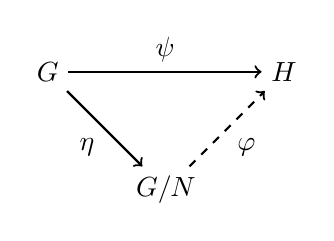
\begin{tikzpicture}
\node (G) at (0,0) {$G$};
\node (H) at (3,0) {$H$};
\node (N) at (1.5, -1.5) {$G/N$};
\draw[thick,  ->] (G) -- (H) node[midway, above] {$\psi$};
\draw[thick, ->] (G) -- (N) node[midway, below left] {$\eta$};
\draw[thick, dashed, ->] (N) -- (H) node[midway, below right] {$\varphi$};
\end{tikzpicture}
\end{center}
\end{multicols}
\end{Thm}
\begin{pf}
The construction of the map $\varphi : G/N\to H$ is also natural in the regard that there is really only one choice to define $\varphi$, that is, we define $\varphi(gN) = \psi(g)$. We first check that this is well-defined. Let $h\in gN$. Then there exists some $n\in N$ such that $h = gn$. Then 
\[\varphi(hN) = \psi(h) = \psi(gn) = \psi(g)\psi(n) = \psi(g)e = \psi(g) = \varphi(gN).\] Therefore, the map $\varphi$ is well-defined. It is also a homomorphism since if $gN, hN\in G/N$ then
\[\varphi(gN\cdot hN) = \varphi(ghN) = \psi(gh) = \psi(g)\psi(h) = \varphi(gN)\varphi(hN).\]

 It also has the property that 
\[\psi(g) = \varphi(gN) = \varphi(\eta(g)) = \varphi\circ\eta(g)\] for all $g\in G$. Thus, $\psi = \varphi\circ \eta$.\\

Suppose that $\chi : G/N \to H$ has the property that $\psi = \chi \circ \eta$. Then $\varphi(gN) = \psi(g) = \chi\circ \eta(g) = \chi(gN)$ for all $gN\in G/N$. Thus, $\varphi = \chi$, which shows that $\varphi$ is the unique such map.\\

Finally, we show that $\varphi$ is injective. Suppose that $\varphi(gN) = e$. But this implies that $\psi(g) = e$, that is, $g\in \ker \psi$. Since $N =  \ker\psi$, we conclude that $g\in N$ and $gN = N$, the identity of $G/N$. Thus, $\ker\varphi = \{N\}$, which shows that $\varphi$ is one-to-one. Since every function maps its domain onto its image, we conclude that $\varphi : G/N \to \im(\psi)$ is an isomorphism. 
\end{pf}\vs

The above diagram is referred to as a \textbf{commutative diagram} because all paths from $G$ to $H$ are equal. The dashed line implies that $\varphi$ is uniquely constructed from $\psi$.\\

The First Isomorphism Theorem shows us that images of homomorphisms correspond to factor groups. It also provides a tool to show us when a $G/N \cong H$, exactly when an epimorphism $G \to H$ exists.

\begin{Exam} Let $\Z \to \Z_n$ be given by the map $m\mapsto m \pmod n$. As seen before, this is a surjective homomorphism and the kernel of this map is $n\Z$. Therefore, $\Z/n\Z \cong \Z_n$.
\end{Exam}\vs

\begin{Exam} Define $\psi : \R \to S^1$ using the map $\varphi(\theta) = e^{2\pi i \theta}$. Then this map is a surjective homomorphism with $\ker \psi = \Z$. Therefore, $\R/\Z \cong S^1$. Similarly, $\Q/\Z$ is isomorphic to the group of all roots of unity, which is a subgroup of $S^1$.\end{Exam}\vs

\vfill
\stepcounter{footnote}\footnotetext{See \href{http://abstract.ups.edu/aata/homomorph-section-group-homomorphisms.html}{\S 11.1 Group Homomorphisms} and \href{http://abstract.ups.edu/aata/homomorph-section-group-isomorphism-theorems.html}{\S 11.2 The Isomorphism Theorems} in Judson's \href{https://judsonbooks.org/aata/}{Abstract Algebra: Theory and Applications} for additional reading.}

\pagebreak

\startExercises{kernel}
For Exercises \ref{exer:kernel:start}--\ref{exer:kernel:stop}, determine the kernel of the given homomorphism.
\begin{enumerate}[!HW!]
\begin{multicols}{2}
\item\label{exer:kernel:start} $\varphi : \Z\to \Z : n\mapsto 7 n$
\item $\varphi : \Z_{18} \to \Z_{24} : n\mapsto 4n$
\end{multicols}
\begin{multicols}{2}
\item $\varphi : \R^*\to \GL_2(\R): \bb x\mapsto \ptx{rr}{1&0\\0&x}$
\item $\varphi : \R\to \GL_2(\R): \bb x\mapsto \ptx{rr}{1&0\\x&1}$
\end{multicols}
\begin{multicols}{2}
\item $\varphi : M_2(\R)\to \R : \ptx{rr}{a&b\\c&d}\mapsto a+d$
\item\label{exer:kernel:stop} $\varphi : M_2(\R)\to \R: \ptx{rr}{a&b\\c&d} \mapsto b$
\end{multicols}
\end{enumerate}

\begin{enumerate}[!HW!]
\item Prove \thmref{thm:ker1-1}.
\item Given a group homomorphism $\varphi : G\to H$, define a relation $\sim$ on $G$ such that $x\sim y$ if and only if $\varphi(x)=\varphi(y)$. Then $\sim$ is an equivalence relation on $G$ and the equivalence classes are the cosets of $\ker\varphi$.
\item Prove or disprove: $\Q/\Z \cong \Q$
\item\label{exer:2ndiso:disprove} Let $\varphi:G_1\to G_2$ be a surjective group homomorphism. Let $H_1\trianglelefteq G_1$ and $H_2=\varphi(H_1)$. Prove or disprove: $G_1/H_1\cong G_2/H_2$.
\end{enumerate}
\vfill
\pagebreak

%%%%%%%%%%%% Section 8.5 %%%%%%%%%%%%%%%%%%%%%%%%%%%%%%%%%%%%%%%%%%%%%%%%%%%%%%%%%%
%%%%%%%%%%%%%%%%%%%%%%%%%%%%%%%%%%%%%%%%%%%%%%%%%%%%%%%%%%%%%%%%%%%%%%%%%%%%
\begin{center} 
\emph{``By three methods we may learn wisdom: First, by reflection, which is noblest; Second, by imitation, which is easiest; and third by experience, which is the bitterest.'' -- Confucius}
\end{center}

\begin{Videos}
\video{https://youtu.be/mEuehapUSzo}{The Product of Subgroups\\ is a Subgroup} &
\video{https://youtu.be/5PARQdKeg84}{The Second\\ Isomorphism Theorem} &
\video{https://youtu.be/JlnwlRxtQyo}{The Third\\ Isomorphism Theorem} &
\video{https://youtu.be/Yp7BtDDlZwA}{The Correspondence\\ Theorem} 
\end{Videos}

\sectionlabel{The Isomorphism Theorems}{isothm}
\begin{Prop} Let $G$ be a group with subgroup $H$ and normal subgroup $N$. Then $HN\le G$. If $H\trianglelefteq G$, then $HN \trianglelefteq G$.\end{Prop}
\begin{pf}
Since $e\in H, N$, then $e = ee \in HN$. Let $x,y\in HN$. Then there exist $h,h'\in H$ and $n,n'\in N$ such that $x=hn$ and $y=h'n'$. Also, since $N$ is normal, we have $h'N = Nh'$, that is, there exists some $n''\in N$ such that $nh' = h'n''$. Then
\[xy = (hn)(h'n') = h(nh')n' = h(h'n'')n' = (hh')(n''n') \in HN,\] since $hh'\in H$ and $n''n'\in N$. So, $HN$ is closed under multiplication. Finally, since $h^{-1}N = Nh^{-1}$ there exists some $n'''\in N$ such that $n^{-1}h^{-1} = h^{-1}n'''$. Then 
\[x^{-1} = (hn)^{-1} = n^{-1}h^{-1} = h^{-1}n'''\in HN,\] which shows that $HN$ contains inverse. Therefore, $HN\le G$. \\

Suppose $H\trianglelefteq G$. Let $g\in G$. Then 
\[gxg^{-1} = g(hn)g^{-1} = gh(g^{-1}g)ng^{-1} = (ghg^{-1})(gng^{-1}) \in HN,\] since $ghg^{-1}\in H$ and $gng^{-1}\in N$. Therefore, $HN$ is closed under conjugation.
\end{pf}\vs

\begin{Thm}[Second Isomorphism Theorem] Let $G$ be a group with subgroup $H$ and normal subgroup $N$. Then 
\[HN/N \cong H/(H\cap N).\]
\end{Thm}
Note that since $N\trianglelefteq G$, $N$ contains all $G$-conjugates of elements from $N$. In particular, $N$ contains all $H$-conjugates of elements from $N$. So, $N\trianglelefteq HN$. So, $HN/N$ is well-defined. Similarly, we have shown previously that $H\cap N\trianglelefteq H$. So, $H/(H\cap N)$ is also well-defined. 
\begin{pf} 
We will prove the Second Isomorphism Theorem using the First Isomorphism Theorem. Let $K = H\cap N$, and define the map $\varphi : HN \to H/K$ by the rule $\varphi(hn) = hK$. Suppose that $h,h' \in H$ and $n, n'\in N$ such that $hn = h'n'$. Then we have that $(h')^{-1}h  = n'(n^{-1})$, and if we let $x = (h')^{-1}h  = n'(n^{-1})$, then  $x\in H\cap N$. Thus, 
\[\varphi(h'n') = h'K = (h'x)K = hK = \varphi(hn).\] This shows that the map is well-defined.\\

Next we see that $\varphi$ is homomorphic, namely  
\[\varphi((hn)(h'n')) = \varphi(hh'n''n') = (hh')K = (hK)(h'K) = \varphi(hn)\varphi(h'n').\] The map $\varphi$ is clearly surjective by construction ($he\mapsto hK$). Finally, if $hn\mapsto K$, then $h\in K=H\cap N$, that is, $h\in N$. This implies that $\ker \varphi = N$ since also $n= en\mapsto eK = K$. Therefore, the First Isomorphism Theorem implies that $HN/N\cong H/K$.
\end{pf}\vs

\begin{Exam} Let $G = S_4$, $N= V_4$, and $H = \langle (123), (12)\rangle = S_3$. Then $|HN| = \dfrac{|H||N|}{|H\cap N|} = \dfrac{6\cdot 4}{1} = 24$, since $H\cap N = \{1\}$. But the only subgroup of $S_4$ of order 24 is $S_4$ itself. Therefore, $\dfrac{S_4}{V_4}  = \dfrac{HN}{N} \cong \dfrac{H}{H\cap N} = \dfrac{S_3}{\{1\}} \cong S_3$, by the Second Isomorphism Theorem.
\end{Exam}\vs

\begin{Thm}[Third Isomorphism Theorem] Let $G$ be a group and $H$ and $N$ are normal subgroups of $G$ with $N\le H$. Then 
\[\dfrac{G/N}{H/N} \cong G/H.\]
\end{Thm}
Note that since $H\trianglelefteq G$, $H$ contains all $G$-conjugates of elements from $H$, that is, $ghg^{-1}\in H$ for all $g\in G$ and $h\in H$. Then $(gN)(hN)(gN)^{-1} = (ghg^{-1})N \in H/N$ since $ghg^{-1}\in H$. Thus, $H/N$ contains all $G/N$-conjugates of elements from $H/N$. So, $H/N\trianglelefteq G/N$. So, $\dfrac{G/N}{H/N}$ is well-defined. 

\begin{pf}
We will also prove the Third Isomorphism Theorem using again the First Isomorphism Theorem. Define a map $\varphi : G/N \to G/H$ by the rule $gN \mapsto gH$. Suppose that $x\in gN$, that is, there exists some $n\in N$ such that $x=gn$. Since $N\le H$, we know that $n\in H$. Then 
\[\varphi(xN) = xH = (gn)H = gH = \varphi(gN).\] Therefore, $\varphi$ is well-defined. It is also homomorphic since if $gN, xN\in G/N$ then 
\[\varphi(gN\cdot xN) = \varphi((gx)N) = (gx)H = (gH)(xH) = \varphi(gN)\varphi(xH).\] We can also see by construction that $\varphi$ is surjective ($gN\mapsto gH$). Thus, it suffices to check that $\ker\varphi = H/N$. This is immediate since $\varphi(gN)= gH = H$ if and only if $g\in H$. Therefore, by the First Isomorphism Theorem, $\dfrac{G/N}{H/N} \cong G/H$.
\end{pf}\vs

\begin{Exam} The groups $\dfrac{\Z/mn\Z}{m\Z/mn\Z} \cong \Z/m\Z \cong \Z_m$ by the Third Isomorphism Theorem.\end{Exam}\vs

\begin{Exam} Let $G = S_4$, $H=A_4$, and $N=V_4$. Then $G/H = S_4/A_4 \cong \Z_2$. Conversely, $G/N = S_4/V_4 \cong S_3$, as seen before, and $H/N = A_4/V_4 \cong A_3$, the only subgroup of order 3 in $S_3$. Then $\dfrac{G/N}{H/N} = \dfrac{S_4/V_4}{A_4/V_4} \cong \dfrac{S_3}{A_3} \cong \Z_2 \cong S_4/A_4$, which was to be expected by the Third Isomorphism Theorem.
\end{Exam}\vs

The final theorem of this section, sometimes called the ``Fourth Isomorphism Theorem,'' is called the Correspondence Theorem. It essentially says that homomorphisms preserve Hasse diagrams.

\begin{Thm}[Correspondence Theorem] Let $N$ be a normal subgroup of a group $G$. Then there is a one-to-one correspondence between the set of subgroups of $G$ containing $N$ and the set of subgroups of $G/N$, namely $H\mapsto H/N$ is a bijective map. Furthermore, this correspondence restricts to a one-to-one correspondence between the set of normal subgroups of $G$ containing $N$ and the set of normal subgroups of $G/N$.
\end{Thm}
\begin{pf}
Let $\eta : G \to G/N$ be the natural map. Let $H\le G$ such that $N\le H$. Then $H/N \le G/N$ since $\eta$ is a homomorphism and, in fact, every subgroup of $G/N$ is of this form since $\eta$ is surjective. Therefore, the natural map establishes a correspondence between the subgroups of $G$ containing $N$ and the subgroups of $G/N$, namely $\eta : H\mapsto H/N$. Furthermore, $H = \eta^{-1}(H/N)$, the pre-image of $H/N$ with respect to $\eta$. Since this correspondence has an inverse, it must be bijective. Therefore, $\eta$ is a one-to-one correspondence. Finally, if $H/N\trianglelefteq G/N$, then we know that $H = \eta^{-1}(H/N) \trianglelefteq G$. Conversely, if $H\trianglelefteq G$, then $H/N = \eta(H) \trianglelefteq G/N$ since $\eta$ is surjective. Thus, $\eta$ restricts to a one-to-one correspondence on normal subgroups.
\end{pf}\vs

\begin{Exam} Note that $V_4 \trianglelefteq S_4$. There are six subgroups of $S_4$ which contain $V_4$, namely $S_4, A_4, V_4$ and three subgroups isomorphic to $D_4$: $\langle (1234), (12)(34)\rangle$, $\langle (1342), (13)(42)\rangle$, and $\langle (1423), (14)(23)\rangle$. The first three groups are normal while the three dihedral groups are not normal. The Hasse diagrams for $S_4$ and $S_4/V_4\cong S_3$ are illustrated below, where normal subgroups are highlighted in red. The Correspondence Theorem guarantees that these Hasse diagrams are isomorphic.\vspace{-0.2 in}

\begin{multicols}{2}
\begin{center}
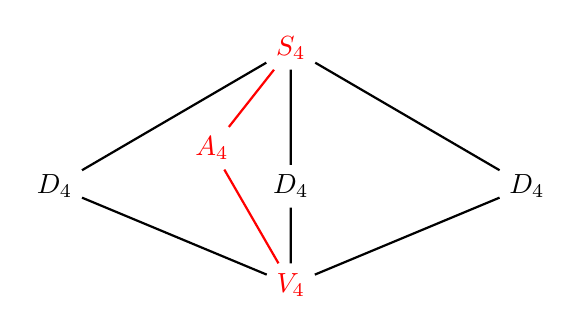
\begin{tikzpicture}
\node[red] (v4) at (0,0) {$V_4$};
\node[red] (a4) at (120:2) {$A_4$};
\node (d4a) at (-3,1.25) {$D_4$};
\node (d4b) at (0,1.25) {$D_4$};
\node (d4c) at (3,1.25) {$D_4$};

\node[red] (s4) at (0,3) {$S_4$};

\draw[thick] (v4) -- (d4a) -- (s4) -- (d4b) -- (v4) -- (d4c) -- (s4);
\draw[thick, red] (v4) -- (a4) -- (s4);

\end{tikzpicture}
\end{center}

\begin{center}
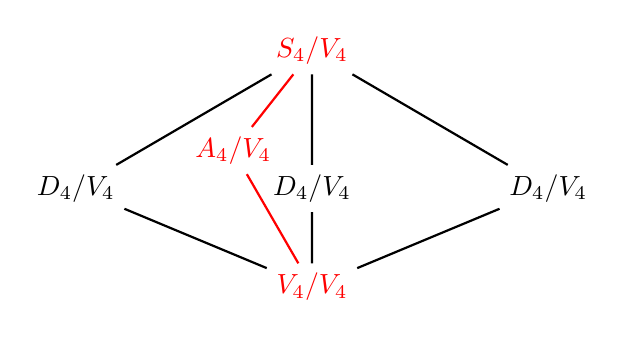
\begin{tikzpicture}
\node[red] (v4) at (0,0) {$V_4/V_4$};
\node[red] (a4) at (120:2) {$A_4/V_4$};
\node (d4a) at (-3,1.25) {$D_4/V_4$};
\node (d4b) at (0,1.25) {$D_4/V_4$};
\node (d4c) at (3,1.25) {$D_4/V_4$};

\node[red] (s4) at (0,3) {$S_4/V_4$};

\draw[thick] (v4) -- (d4a) -- (s4) -- (d4b) -- (v4) -- (d4c) -- (s4);
\draw[thick, red] (v4) -- (a4) -- (s4);

\end{tikzpicture}
\end{center}
\end{multicols}
\end{Exam}

\vfill
\stepcounter{footnote}\footnotetext{See  \href{http://abstract.ups.edu/aata/homomorph-section-group-isomorphism-theorems.html}{\S 11.2 The Isomorphism Theorems} in Judson's \href{https://judsonbooks.org/aata/}{Abstract Algebra: Theory and Applications} for additional reading.}

\pagebreak

\startExercises{isothm}
\begin{enumerate}[!HW!]
\item Let $G=\Z_{24}$, $H=4\Z_{24}$, and $N=6\Z_{24}$. List all elements of $H+N$, $H\cap N$, $(H+N)/N$, and $H/(H\cap N)$. Give the correspondence between $(H+N)/N$ and $H/(H\cap N)$, as given in the 2nd Isomorphism Theorem.
\item Show that a group homomorphism whose domain is a cyclic group is completely determined by the image on a generator of the domain.
\item Let $G$ be a group and $N\trianglelefteq G$. If $H\le G/N$, prove that $\eta^{-1}(H)\le G$ of order $|H||N|$, where $\eta : G\to G/N$ is the natural map.
\item Let $G_1$ and $G_2$ be groups such that $N_1\trianglelefteq G_1$ and $N_2\trianglelefteq G_2$. Let $\varphi : G_1\to G_2$ be a group homomorphism. If $\varphi(N_1)\le N_2$, Prove that there exists a homomorphism $\overline{\varphi} : G_1/N_1\to G_2/N_2$ such that $\eta\circ \varphi = \overline{\varphi}\circ \eta$, where $\eta$ is the natural map.
\item If $H,K\trianglelefteq G$ and $H\cap K =\{e\}$, prove that $G$ is isomorphic to a subgroup of $G/H\times G/K$.
\end{enumerate}
\vfill
\pagebreak
%%%%%%%%%%%% Supplementary Exercises %%%%%%%%%%%%%%%%%%%%%%%%%%%%%%%%%%%%%%%%%%%%%%%%%%%%%%%%%%
%%%%%%%%%%%%%%%%%%%%%%%%%%%%%%%%%%%%%%%%%%%%%%%%%%%%%%%%%%%%%%%%%%%%%%%%%%%%
\startSuppExercises{homomorphism}

\begin{enumerate}[!HW!]
\item Let $G = \left\{\ptx{rr}{a&b\\0&c}\ \middle|\ a,b,c\in \R\right\}\le \GL_2(\R)$. Let $H =\left\{\ptx{rr}{1&b\\0&1}\ \middle|\ b\in \R\right\}\subseteq G$. Show that $H$ is an abelian subgroup of $G$,   $H\trianglelefteq G$, and $G/H \cong \R^*\times \R^*$.
\item If $G$ is a group and $H\le G$ such that $[G:H] = 2$, then $H\trianglelefteq G$.
\item Prove or disprove: If $G$ is a group, $H\trianglelefteq G$, $H$ is abelian, and $G/H$ is abelian, then $G$ is abelian.
\item Prove that $\det : \GL_2(\R) \to \R^*$ is a group homomorphism. What is its kernel?
\end{enumerate}
\pagebreak
%%%%%%%%%%%% CHAPTER 9 %%%%%%%%%%%%%%%%%%%%
%%%%%%%%%%%%%%%%%%%%%%%%%%%%%%%%%%%%%%%%%%%%%%%%%%%%%%%%%%%%%%%%%%%%%%%%%%%%%%%%
\chapterlabel{Representation Theory}{representation}\pagebreak
%%%%%%%%%%%% Section 9.1 %%%%%%%%%%%%%%%%%%%%%%%%%%%%%%%%%%%%%%%%%%%%%%%%%%%%%%%%%%
%%%%%%%%%%%%%%%%%%%%%%%%%%%%%%%%%%%%%%%%%%%%%%%%%%%%%%%%%%%%%%%%%%%%%%%%%%%%
\begin{center} 
\emph{``Your expectations opens or closes the doors of your supply, If you expect grand things, and work honestly for them, they will come to you, your supply will correspond with your expectation.'' -- Orison Swett Marden}
\end{center}

\begin{Videos}
\video{https://youtu.be/HELC_KI7F1Y}{The Classical Matrix Groups} &
\video{https://youtu.be/jeYa2ce88XM}{The Orthogonal Group} &
\video{https://youtu.be/Qnkv-M0pkNE}{The Unitary Group} 
\end{Videos}

\sectionlabel{The Classical Matrix Groups}{matrix}
In this section, we will present the classical matrix groups. We have seen some already, namely the \emph{general linear groups} $\GL_n(\R)$ and $\GL_n(\C)$, the groups of nonsingular $n\times n$ matrices with real or complex scalar with matrix multiplication. We have seen already that since $\det$ is a homomorphism from the general linear group, that is, 
\[\det(AB) = \det(A)\det(B),\] its kernel is a normal subgroup, namely the \emph{special linear groups} $\SL_n(\R)$ and $\SL_n(\C)$. \\

Recall from linear algebra the \emph{transpose} operator  $\,^\top : A = (a_{ij}) \mapsto A^\top = (a_{ji})$. The following properties are also standard from linear algebra:
\begin{multicols}{3}
\begin{enumerate}[!THM!,start=1]
\item $(A+B)^\top = A^\top + B^\top$\\
\item $(rA)^\top = rA^\top$\\
\item $(A^\top)^\top = A$\\
\item $(AB)^\top = B^\top A^\top$\\
\item $\det(A^\top) = \det(A)$\\
\end{enumerate}
\end{multicols}\vspace{-0.15 in}

\begin{Def}
Define the set $O(n)$ (or $O_n(\R)$), called the \textbf{orthogonal group}, as the subset of \emph{orthogonal matrices}, those invertible real matrices whose inverse is equal to its transpose. In other words, 
\[O(n) = \{Q\in \GL_n(\R)\mid Q^\top = Q^{-1}\}.\] It is an exercise of the reader to show that $O(n) \le \GL_n(\R)$.
\end{Def}\vs

Note that if $Q^{-1} = Q^\top$, then it must be that $QQ^{T} = QQ^{-1} =I_n$. Likewise, $Q^\top Q = I_n$.

%\begin{Prop} The set $O(n)$ is a subgroup of $\GL_n(\R)$.\end{Prop}
%\begin{proof}
%Let $Q, P \in O(n)$. Then 
%\[(QP)(QP)^\top = QPP^\top Q^\top = QPP^{-1}Q^{-1} = QQ^{-1} = I_n.\] Similarly, $(QP)^\top(QP) = I_n$. Thus, $O(n)$ is closed under multiplication. Since $I_n^\top = I_n$, we have $I_nI_n^\top = I_n^\top I_n= I_nI_n = I_n$. Thus, $I_n\in O(n)$. Finally, if $Q\in O(n)$ then $QQ^\top = Q^\top Q = I_n$. But this implies that $(Q^\top)^\top Q^\top = Q^\top(Q^\top)^\top = I_n$. Hence, $Q^{-1}=Q^\top$ is orthogonal and $Q^{-1}\in O(n)$. Therefore, $O(n)\le \GL_n(\R)$.\end{proof}\vs

\begin{Thm} A square matrix $U$ is orthogonal if and only if its column vectors form an orthonormal set.\end{Thm}
\begin{pf}
Let $U$ be an $n\times n$ orthogonal matrix and let $\bb u_1, \bb u_2,\ldots, \bb u_n$ be the column vectors of $U$. Then
\[U^\top U = (u_{ij})^\top(u_{ij}) =(\bb u_i^\top\bb u_j) = (\bb u_i\cdot \bb u_j).\] Therefore, $U^\top U = I_n$ if and only if $\bb u_i\cdot \bb u_j = \begin{cases} 0, & i\neq j\\ 1, & i=j\end{cases}$ if and only if the columns of $U$ are an orthonormal set.
\end{pf}\vs

Since $U^\top = U^{-1}$ and $UU^\top = UU^{-1} = I$, it also follows that the row vectors of an orthogonal matrix $U$ must also form an orthonormal set.\\

Geometrically speaking, the orthogonal group $O(n)$ consists of all rotation and reflection matrices of $\R^n$.\\

\begin{Exam}\label{exam:1} The matrix 
\[U = \mtx{rrr}{3/\sqrt{11} & -1/\sqrt{6} & -1/\sqrt{66}\\ 1/\sqrt{11} & 2/\sqrt{6} & -4/\sqrt{66}  \\ 1/\sqrt{11} & 1/\sqrt{6} & 7/\sqrt{66}}\] is an orthogonal matrix. Note that 
\[U^\top U = \mtx{rrr}{3/\sqrt{11} & 1/\sqrt{11} & 1/\sqrt{11}\\ -1/\sqrt{6} & 2/\sqrt{6} & 1/\sqrt{6}  \\ -1/\sqrt{66} & -4/\sqrt{66} & 7/\sqrt{66}}\mtx{rrr}{3/\sqrt{11} & -1/\sqrt{6} & -1/\sqrt{66}\\ 1/\sqrt{11} & 2/\sqrt{6} & -4/\sqrt{66}  \\ 1/\sqrt{11} & 1/\sqrt{6} & 7/\sqrt{66}}\] \[= \mtx{ccc}{(9+1+1)/11 & (-3+2+1)/\sqrt{66} & (-3-4+7)/\sqrt{726} \\ (-3+2+1)/\sqrt{66} & (1+4+1)/6 & (1-8+7)/\sqrt{396} \\ (-3-4+7)/\sqrt{726} & (1-8+7)/\sqrt{396} & (1+16+49)/66} = I_3\qedhere\]
\end{Exam}\vs

\begin{Thm} Let $U$ be an orthogonal matrix, and let $\bb x, \bb y \in \R^n$. Then \[(U\bb x)\cdot (U\bb y) = \bb x\cdot \bb y,\] that is, the matrix transformation $\bb x\mapsto \bb U\bb x$ preserves inner products.
\end{Thm}
\begin{pf}
\[(U\bb x)\cdot (U\bb y) = (U\bb x)^\top(U\bb y) =(\bb x^\top U^\top)(U\bb y)  = \bb x^\top(U^\top U)\bb y = \bb x^\top\bb y  = \bb x \cdot \bb y.\qedhere\]
\end{pf}\vs

Since multiplication by an orthogonal matrix $U$ preserves dot product, as a consequence, it also preserves lengths, distances, angles, and orthogonality of vectors. For example, $\Vert U\bb x \Vert = \Vert \bb x\Vert$ for any vector $\bb x$ and any orthogonal matrix $U$. In particular, orthogonal matrices are exactly those linear transformations of $\R^n$ that preserve lengths, called a \textbf{rigid motion}.\\


Let $SO(n)$ (or $SO_n(\R)$), called the \textbf{special orthogonal group}, as the subset of orthogonal matrices with determinant equal to 1, that is, $SO(n) = O(n) \cap \SL_n(\R)$. This implies that $SO(n) \trianglelefteq O(n)$. It can be shown that $\det(Q) = \pm 1$ for all $Q\in O(n)$. A consequence of this fact is that $[O(n) : SO(n)] = 2$, which also shows that it is normal in the orthogonal groups. \\

For complex matrices, we define the notion of the ``orthogonal'' group differently. In particular, the dot product $\bb u \cdot \bb v = \bb u^\top\bb v$ does not quite work the correct way anymore. For example, $\vr{1 \\ i } \cdot \vr{1\\i} = 1-1 = 0$ but $\vr{1\\i} \neq \bb 0$. To repair this problem, the dot product on complex spaces is replaced with the \emph{Hermitian product}.

\begin{Def} Let $A$ be an $m\times n$ complex matrix. Then we define $A^* = (\overline{A})^\top$, which is called the \textbf{conjugate transpose}. This replaces the role of transposes in complex space.
\end{Def}\vs

\begin{Exam} Let $A = \mtx{ccc}{ 1+i & -i & 0 \\ 2 & 3-2i & i}$ and  $B = \mtx{ccc}{1 & i & 1+i \\ -i & -5 & 2-i \\ 1-i & 2+i & 3}$.\\

  Note that 
\[A^* = \mtx{cc}{1-i & 2 \\ i & 3+2i \\ 0 & -i},\qquad B^* =  \mtx{ccc}{1 & i & 1+i \\ -i & -5 & 2-i \\ 1-i & 2+i & 3}. \qedhere \]
\end{Exam}\vs

\begin{Def}
We define the \textbf{Hermitian product}\footnotemark\ $\cdot : \C^n\times \C^n \to \C$ of two vectors, $\bb u, \bb v \in \C^n$ by the rule
\[\bb u \cdot \bb v = \bb u^* \bb v = \mtx{cccc}{\overline{u_1} & \overline{u_2} & \ldots & \overline{u_n}}\mtx{c}{v_1 \\ v_2 \\ \vdots \\ v_n} = \overline{u_1}v_1 + \overline{u_2}v_2 + \ldots + \overline{u_n}v_n.\]
\end{Def}\vs

The concepts of vector norms (lengths), vector distance, unit vectors, normalizations, angles, etc. that were defined via the dot product can naturally be extended to complex vector space via the Hermitian product.

\begin{Exam} Let $\bb u = (1+i,\ i,\ 3-i)$ and $\bb v = (1+i,\ 2,\ 4i)$. Find $\bb u\cdot \bb v$, $\bb v\cdot \bb u$, and $\Vert \bb u\Vert$.

\[\bb u\cdot \bb v = (\overline{1+i})(1+i) + \overline{i}(2) + (\overline{3-i})(4i) = (1-i)(1+i) - 2i + (3+i)(4i) = 2 - 2i + 12i - 4 = \fbox{$-2+10i$}\]
\[\bb v \cdot \bb u = (\overline{1+i})(1+i) + \overline{2}(i) + (\overline{4i})(3-i) = (1-i)(1+i) + 2i - (4i)(3-i) = 2 + 2i - 12i - 4 = \fbox{$-2 - 10i$}\]
\begin{multline*}\Vert \bb u\Vert = \sqrt{(\overline{1+i})(1+i) + (\overline{i})i + (\overline{3-i})(3-i)} = \sqrt{ (1-i)(1+i) + (-i)i + (3+i)(3-i)}\\ = \sqrt{2 + 1 + 10} = \fbox{$\sqrt{13}$}
\end{multline*}
\end{Exam}\vs


\begin{Thm}\label{thm:complexvector} Let $\bb u, \bb v, \bb w\in \C^n$ and let $z\in \C$. Then
\begin{multicols}{2}
\begin{enumerate}[!THM!,start=1]
\item\label{1} $\bb u \cdot \bb v = \overline{\bb v \cdot \bb u}$;
\item $(\bb u + \bb v)\cdot \bb w = \bb u \cdot \bb w  + \bb v \cdot \bb w$;
\item $\bb u \cdot (\bb v + \bb w) = \bb u \cdot \bb v  + \bb u \cdot \bb w$;
\item\label{4} $(z\bb u)\cdot \bb v = \overline{z}(\bb u\cdot \bb v)$;
\item $\bb u\cdot (z\bb v) = z(\bb u\cdot \bb v)$;
\item\label{6} $\bb u \cdot \bb u \ge 0$, and $\bb u \cdot \bb u = 0$ if and only if $\bb u = \bb 0$.
\end{enumerate}
\end{multicols}
\end{Thm}\vs

\begin{Def}
Define the set $U(n)$ (or $U_n(\C)$), called the \textbf{unitary group}, as the subset of \emph{unitary matrices}, those invertible complex matrices whose inverse is equal to its conjugate transpose. In other words, 
\[U(n) = \{U\in \GL_n(\C)\mid Q^* = Q^{-1}\}.\] Note that $U\in U(n)$ if and only if $U^*U = UU^* = I_n$.\\

The \textbf{special unitary group} $SU(n)$ is the subgroup of $U(n)$ whose determinants are 1.
\end{Def}\vs

\begin{Exam} Let $U = \mtx{cc}{ \frac{1}{2}(1+i) & \frac{1}{2}(1+i) \\ \frac{1}{2}(1-i) & \frac{1}{2}(-1+i)}$.\\

  Note that 
\[UU^* = \mtx{cc}{ \frac{1}{2}(1+i) & \frac{1}{2}(1+i) \\ \frac{1}{2}(1-i) & \frac{1}{2}(-1+i)}\mtx{cc}{ \frac{1}{2}(1-i) & \frac{1}{2}(1+i) \\ \frac{1}{2}(1-i) & \frac{1}{2}(-1-i)} = \mtx{cc}{\frac{1}{2} + \frac{1}{2} & \frac{i}{2} - \frac{i}{2} \\ -\frac{i}{2} + \frac{i}{2} & \frac{1}{2} + \frac{1}{2}} = I_2\]

Therefore, $U$ is unitary.
\end{Exam}\vs

Analogously, unitary matrices are exactly the complex matrices that preserve Hermitian products, and thus also preserve lengths and distances. In other words, $U(n)$ is the group of rigid motions of $\C^n$.\\

\vfill
\footnotetext{Many textbooks alternatively define the Hermitian product as $\bb u \cdot \bb v =  \bb u^\top\overline{\bb v}$. Although this does not at all change the theory and applications of the Hermitian product, it does change intermediate calculations.}
\stepcounter{footnote}\footnotetext{See  \href{http://abstract.ups.edu/aata/matrix-section-groups.html}{\S 12.1 Matrix Groups} in Judson's \href{https://judsonbooks.org/aata/}{Abstract Algebra: Theory and Applications} for additional reading.}

\pagebreak

\startExercises{matrix}
For Exercises \ref{exer:specialorthogonalmatrix:start}--\ref{exer:specialorthogonalmatrix:stop}, determine whether the matrix $A$ belongs to $O(n)$ or $SO(n)$.
\begin{enumerate}[!HW!]
\begin{multicols}{2}
\item\label{exer:specialorthogonalmatrix:start} $\ptx{rr}{\tfrac{1}{\sqrt{2}}&-\tfrac{1}{\sqrt{2}}\\\tfrac{1}{\sqrt{2}}&\tfrac{1}{\sqrt{2}}}$ %SO
\item $\ptx{rr}{\tfrac{1}{\sqrt{5}}&\tfrac{2}{\sqrt{5}}\\\-\tfrac{2}{\sqrt{5}}&\tfrac{1}{\sqrt{5}}}$%SO
\end{multicols}
\begin{multicols}{2}
\item $\ptx{rrr}{\tfrac{4}{5}&0&\tfrac{3}{5}\\-\tfrac{3}{5}&0&\tfrac{4}{5}\\0&-1&0}$%O
\item\label{exer:specialorthogonalmatrix:stop} $\ptx{rrr}{\tfrac{1}{3}&\tfrac{2}{3}&-\tfrac{2}{3}\\-\tfrac{2}{3}&\tfrac{2}{3}&\tfrac{1}{3}\\\tfrac{2}{3}&\tfrac{1}{3}&\tfrac{2}{3}}$
\end{multicols}
\end{enumerate}

\begin{enumerate}[!HW!]
\item Prove that $O(n)$ is a group.
\item Prove that $SU(n)\trianglelefteq U(n)$.
\item Prove or disprove: there exists an infinite abelian subgroup of $O(n)$.
\item Let $\bb x\in \R^n$ such that $\Vert \bb x\Vert=1$, that is, $\bb x\in S^{n-1}$, where $S^{n-1}$ is the unit $n-1$ sphere. If $U\in O(n)$, prove that $U\bb x\in S^{n-1}$.
\end{enumerate}
\vfill
\pagebreak

%%%%%%%%%%%% Section 9.2 %%%%%%%%%%%%%%%%%%%%%%%%%%%%%%%%%%%%%%%%%%%%%%%%%%%%%%%%%%
%%%%%%%%%%%%%%%%%%%%%%%%%%%%%%%%%%%%%%%%%%%%%%%%%%%%%%%%%%%%%%%%%%%%%%%%%%%%
\begin{center} 
\emph{`Never mistake motion for action.'' -- Ernest Hemingway}
\end{center}

\begin{Videos}
\video{https://youtu.be/2glDngQCvTA}{Symmetries} &
\video{https://youtu.be/4S6XwBhDLHE}{ Symmetries of Euclidean Space $\R^n$} 
\end{Videos}

\sectionlabel{Isometries}{isometry}
Recall that a \textbf{symmetry} $\sigma : X\to X$ is a permutation which preserves the underlying structure of the object $X$. If $X$ is a set, then the the symmetry group $S_X$ is the collection of all permutations from $X$ into itself. If $X$ has no other structure, this captures all the symmetries of the object $X$. For example, if $X = \{1,2,3,4\}$, then the symmetry group of $X$ is just $S_4$.

\begin{multicols}{2}
But maybe $X$ does have some other structure, for example say that $X = \{1,2,3,4\}$ but these four points are the vertices of a square. Then we will not consider all permutations of $X$ but only those permutations which also preserve the adjacency relations of vertices, that is, those permutations that preserve the shape of the square. Of course, only the permutations in $D_4$ preserve the square-ness of $X$. \columnbreak

\mbox{}
\begin{center}
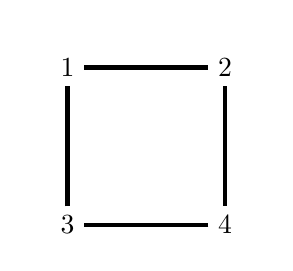
\begin{tikzpicture}
\draw[white] (-0.5,2.5) -- (2.5,2.5);
\path (0,2) node (A) {1};
\path (2,2) node (B) {2};
\path (0,0) node (D) {3};
\path (2,0) node (C) {4};

\draw[ultra thick] (A) -- (B) -- (C) -- (D) -- (A);
\end{tikzpicture}
\end{center}
\end{multicols}

\begin{multicols}{2}
For another example, consider $X = \{1,2,3,4\}$ as a group with the following Cayley table. Of course, $X \cong \Z_4$. In this situation, the symmetries of $X$ as a group are all permutations $\varphi : X\to X$ such that $\varphi$ preserves the group operation, that is, $\varphi(ab) = \varphi(a)\varphi(b)$. Notice that this implies that $\varphi$ is an isomorphism from $X$ to itself. Such an isomorphism is called an \textbf{automorphism}. Viewing $X$ as a group, the symmetry group of $X$ becomes $\langle (24)\rangle = \{1, (24)\}$. \columnbreak

\mbox{}

\begin{center}
  \begin{tabular}{c|cccc}
    & 1 & 2 & 3 & 4 \\\hline
  1 & 1 & 2 & 3 & 4 \\
  2 & 2 & 3 & 4 & 1 \\
  3 & 3 & 4 & 1 & 2 \\
  4 & 4 & 1 & 2 & 3 \\
  \end{tabular}
\end{center}
\end{multicols}

Thus, when we view $X$ as just a set, its symmetry group is $S_4$. When we view $X$ as a square, its symmetry group is $D_4$, a subgroup of $S_4$. When we view $X$ as a cyclic group, its symmetry group is $\Z_2$, another subgroup of $S_4$. In this manner, when we consider the symmetry group of an object we need to focus not just on the elements which create the object but also the relations between the elements that capture the aspects we are focusing on. \\

The Euclidean space $\R^n$ is a beautifully complicated mathematical object, with a deep interplay between both algebra and topology. Algebraically, $\R^n$ is a vector space with vector addition and scalar multiplication. When given the dot product, $\R^n$ becomes an inner product, a stronger algebraic object. But this inner product leads toward the geometry of $\R^n$. With the dot product, we can discuss lengths, distances, and angles. This makes $\R^n$ into a metric space, which forms a topology on $\R^n$ by which we can start discussing convergent sequences, Cauchy sequences, completeness, compactness, limits, derivatives, etc. Based upon the focus we have on $\R^n$, we will discuss the symmetries of this great object.

\begin{Exam}
Viewing $\R^n$ as a vector space, the symmetries of $\R^n$ will be those permutations of $\R^n$ which preserve the vector space structure, namely vector addition and scalar multiplication. Maps that preserve vector addition and scalar multiplications are just \emph{linear transformations} from linear algebra and they are the analog of group homomorphisms for vector space. It is a common fact from linear algebra that any linear transformation $\R^n\to \R^m$ can be represented as an $m\times n$ uniquely using the standard bases. If this linear transformation is bijective, since it is a permutation, then the linear transformation must both be one-to-one and onto. This implies that the standard matrix is nonsingular. Therefore, $\GL_n(\R)$ is symmetry group of $\R^n$ with respect to its vector space structure.
\end{Exam}\vs

\begin{Exam}
Viewing $\R^n$ as an inner product space, the symmetries of $\R^n$ will be those permutations of $\R^n$ which preserve the inner product structure, namely vector addition, scalar multiplication and the inner product. As mentioned before, this symmetry must be an element of $\GL_n(\R)$. As we discussed earlier, a matrix $A$ preserves all dot products if and only if $A$ is orthogonal. Therefore, $O(n)$ is symmetry group of $\R^n$ with respect to its inner product space structure. Geometrically speaking, the $O(n)$ consists of all \emph{rotations} about the origin and \emph{reflections} through the origin or across lines through the origin.
\end{Exam}\vs

\begin{Exam} Because orthogonal matrices preserve dot products, lengths and distances are also preserved. When viewing $\R^n$ as a metric space, our symmetries are all those permutations of $\R^n$ that preserve distance, which are called \textbf{isometries}. Of course, all orthogonal matrices are isometries of $\R^n$, but orthogonal matrices preserve the whole algebraic structure of $\R^n$. A general isometry only needs to preserve the geometric (and topological) structure of $\R^n$. \\

\emph{Rotations} about any point and \emph{reflections} across any line are examples of isometries. These are not linear transformations, and hence not orthogonal matrices, if the point of rotation is not the origin or if the line of reflection does not pass through the origin. Another isometry is \emph{translation} which maps the point $\bb x$ to $\bb x + \bb v$ for some fixed vector $\bb v$. Translations are linear transformations if and only if $\bb v = \bb 0$, in which case the translation is just the identity map. These three types of isometries generate the isometry group of $\R^n$.\\

Define the set $E(n)$ as the Cartesian product of $\R^n$ and $O(n)$, namely $E(n) = \R^n\times O(n)$. We will turn $E(n)$ into a group but not by using the direct product multiplication. Instead, if $\bb u, \bb v\in \R^n$ and $A, B\in O(n)$, then we define multiplication by the rule:
\[(\bb u, A)\circ (\bb v, B) = (\bb u + A\bb v, AB)\in E(n).\] The multiplication forms a group structure on $E(n)$, called the \textbf{Euclidean group}. It is left as an exercise to the reader to prove that $E(n)$ is a group.\\

The Euclidean group $E(n)$ forms the group of distance-preserving-symmetries of $\R^n$ in the following way: let $\bb x, \bb v\in \R^n$ and $A\in O(n)$. Then we define $(\bb v, A) : \R^n \to \R^n$ by the rule $(\bb v, A)\bb x = \bb v + A\bb x\in \R^n$. In particular, $(\bb v, I)$ is simple translation by the vector $\bb v$ and $(\bb 0, A)$ is simple multiplication by the orthogonal matrix $A$.\\

In $\R^2$, $E(2)$ consists of all rotations around a point, reflections across a line, translations, and glide reflections, which is a composite of a translations and a reflection, namely $(\bb v, A)$ where $\bb v \in \R^n$ and $A$ is a reflection matrix. All other elements of $E(2)$ can be expressed as one of these four types. In $\R^3$, the Euclidean group $E(3)$ consists of seven types: translations, rotations around a line, reflections through a point, reflections across a plane, glide reflections,  screw displacements (a composite of a translation and a rotation), and improper rotations (rotation around an axis and reflection through the orthogonal complement). 
\end{Exam}\vs

\begin{Exam} Finally, the topology of $\R^n$ is a weaker structure than the geometry of $\R^n$, that is, a permutation can preserve closeness between two points without necessarily preserving distance. These describe continuous permutations. Define $\text{Aff}(n)$, called the \textbf{Affine group}, to be the Cartesian product $\text{Aff}(n) = \R^n\times \GL_n(\R)$\footnotemark\ and multiplication as the rule:
\[(\bb u, A)\circ (\bb v, B) = (\bb u + A\bb v, AB)\in \text{Aff}(n).\] This forms a group by the same reasoning as the Euclidean group. In fact, $E(n) \le \text{Aff}(n)$. In addition to the types of transformations mentioned above in $E(n)$, $\text{Aff}(n)$ also contains stretches/compressions/dilations and shears, a linear map that displaces each point in fixed direction, by an amount proportional to its signed distance from a hyperplane that is parallel to that direction.
\end{Exam}\vs

\begin{Exam} Is $\SL_n(\R)$ a symmetry group for $\R^n$? Yes, in a way. If $A$ is a $2\times 2$ matrix, the area of the parallelogram determined by the columns of $A$ is $|\det A|$. If $A$ is $3\times 3$, the volume of the parallelepiped determined by the columns of $A$ is $|\det A|$. The higher dimensional analogues also hold. It is left as an exericse that $\SL_n(\R)$ is the symmetry group of $\R^n$ which preserves areas, but does not necessarily preserve distance.
\end{Exam}

\vfill
\footnotetext{Both $E(n)$ and $\text{Aff}(n)$ give examples of \textbf{semi-direct product}, which is an alternative multiplication placed upon a Cartesian product.}
\stepcounter{footnote}\footnotetext{See  \href{http://abstract.ups.edu/aata/matrix-section-symmetry.html}{\S 12.2 Symmetry} in Judson's \href{https://judsonbooks.org/aata/}{Abstract Algebra: Theory and Applications} for additional reading.}

\pagebreak

\startExercises{isometry}
\begin{enumerate}[!HW!]
\item Prove that $E(n)$ is a group for all $n\ge 1$.
\item Prove or disprove: there exists some $(A,\bb x)\in E(2)$ where $\bb x\neq \bb 0$ and $|(A,\bb x)|=\infty$.
\end{enumerate}

\begin{Def} Let $\bb x_1,\ldots, \bb x_k\in \R^n$. Then we say a linear combination $c_1\bb x_1+\ldots+c_k\bb x_k$ is a \textbf{convex combination} if $c_i\ge 0$ for $1\le i\le k$ and $c_1+\ldots +c_k=1$.\\

 Let $X\in \R^n$. Then the \textbf{convex span} (or \textbf{convex hull}), denoted $\text{ConSpan}(X)$, is the set of all convex combinations involving only finitely many vectors in $X$. Note that this is the smallest convex subset of $\R^n$ containing $X$. \\
 
 We say that $X\subseteq \R^n$ is a \textbf{hyper-parallelepiped}\footnotemark\ if $X=\text{ConSpan}\{\bb x_1,\ldots, \bb x_n\}$ for some vectors $\bb x_1,\ldots, \bb x_n\in \R^n$. If $A$ is the $n\times n$ matrix whose columns are $\bb x_1,\ldots, \bb x_n$, then the \textbf{hyper-volume} of the hyper-parallelepiped $X$ is $|\det(A)|$.
 \end{Def}\vs
 
 \begin{enumerate}[!HW!]
 \item Prove that $\SL_n(\R)$ preserves the hyper-volume of each hyper-parallelepiped in $\R^n$.
 \end{enumerate}

\begin{Def} Let $G$ be a group with normal subgroup $H$ and (not necessarily normal) subgroup $K$. If $G=HK$ and $H\cap K = \{e\}$, then we say that $G$ is the \textbf{internal semidirect product} of $H$ and $K$, denoted $G=H\rtimes K$. 
\end{Def}\vs

\begin{enumerate}[!HW!]
\item Prove that $S_3 = A_3\rtimes \langle (12)\rangle$.
\item Prove that $\text{Aff}(n) = R^n\rtimes \GL_n(\R)$. 
\item Prove that $Q_8$ is not a semidirect product of any of its subgroups.
\end{enumerate}

\vfill
\footnotetext{In dimensions $n=1,2,3$, a hyper-parallelepiped is instead called a \textbf{segment}, \textbf{parallelogram}, and \textbf{parallelepiped}, and its hyper-volume is instead called \textbf{length}, \textbf{area}, and \textbf{volume}, respectively.}
\pagebreak
%%%%%%%%%%%% Supplementary Exercises %%%%%%%%%%%%%%%%%%%%%%%%%%%%%%%%%%%%%%%%%%%%%%%%%%%%%%%%%%
%%%%%%%%%%%%%%%%%%%%%%%%%%%%%%%%%%%%%%%%%%%%%%%%%%%%%%%%%%%%%%%%%%%%%%%%%%%%
\startSuppExercises{representation}

\begin{enumerate}[!HW!]
\item Prove \thmref{thm:complexvector}.
\item For all $\bb u, \bb v\in \C^n$, prove
\[\bb u\cdot \bb v = \dfrac{1}{2}\left(\Vert \bb u+\bb v\Vert^2-\Vert \bb u\Vert^2-\Vert\bb v\Vert^2\right).\]
\item Suppose that $G\le E(2) = \R^2\rtimes O(2)$ and let $T=G\cap \R^2$, where $T$ is the translation subgroup of $G$. Prove that $G/T\cong G\cap O(2)$.
\end{enumerate}
\pagebreak

%%%%%%%%%%%% CHAPTER 9 %%%%%%%%%%%%%%%%%%%%
%%%%%%%%%%%%%%%%%%%%%%%%%%%%%%%%%%%%%%%%%%%%%%%%%%%%%%%%%%%%%%%%%%%%%%%%%%%%%%%%
\chapterlabel{Rings}{rngs}\pagebreak

%%%%%%%%%%%% Section 10.1 %%%%%%%%%%%%%%%%%%%%%%%%%%%%%%%%%%%%%%%%%%%%%%%%%%%%%%%%%%
%%%%%%%%%%%%%%%%%%%%%%%%%%%%%%%%%%%%%%%%%%%%%%%%%%%%%%%%%%%%%%%%%%%%%%%%%%%%
\begin{center} 
\emph{``A bell's not a bell `til you ring it, A song's not a song `til you sing it,\\ Love in your heart wasn't put there to stay, Love isn't love `til you give it away!'' -- Oscar Hammerstein II}
\end{center}

\begin{Videos}
\video{https://youtu.be/qRYOpB0es0E}{Rings} &
\video{https://youtu.be/kub-Ub54Myc}{Subrings} &
\video{https://youtu.be/7-eFNBn-Fbk}{The Dominance of\\ Zero in a Ring} &
\video{https://youtu.be/C769JxuOiH4}{Matrix Rings} &
\video{https://youtu.be/mbO072f7vxQ}{Polynomial  Rings} 
\end{Videos}

\sectionlabel{Rings}{rngs}
Up until now, we have focused on algebraic sets with a single binary operation. Often in algebra, it is useful to consider a set with multiple operations that interact with each other nicely, for example vector spaces in linear algebra have two operations: vector addition and scalar multiplication in which scalar multiplication distributes over vector addition. Inner product spaces have a third operation, the inner product, that also behaves nicely with the two other operations of the vector space. Many other operations from linear algebra could be listed, like the cross product and outer product, which behave nicely with the other algebraic operations often in the form of some kind of distributive property or homogeneity property. We have also seen in set theory that binary operations of intersection, union, and set difference are very compatible with each other and other important set operations. \\

The study of algebraic rings is in this vein, that is, a ring is, loosely speaking, an algebraic set with two binary operations, called addition and multiplication, that are compatible (distributive) with each. The precise definition is below.

\begin{Def} We say that $(R,+, \cdot)$ is a \textbf{ring} if the following seven axioms are satisfied by the binary operations:
\begin{enumerate}[!THM!,start=1]
\item (\textbf{additive associativity}) For all $r, s, t \in R$, it holds that 
\[r+ (s + t) = (r + s) + t.\]
\item (\textbf{additive commutativity}) For all $r, s\in R$, it holds that 
\[r + s = s + r.\]
\item (\textbf{additive identity}) There exists an element $0\in R$ such that for all $r\in R$ we have
\[r+ 0 = 0+ r = r.\]
\item (\textbf{additive inverses}) For all $r\in R$ there is an element $(-r)\in R$ such that
\[r + (-r) = (-r) + r = 0.\]

\item (\textbf{multiplicative associativity}) For all $r, s, t \in R$, it holds that 
\[r\cdot (s \cdot t) = (r \cdot s) \cdot t.\] 
\item (\textbf{left distributivity}) For all $r, s, t \in R$, it holds that 
\[r\cdot (s + t) = (r \cdot s) + (r \cdot t).\] 
\item (\textbf{right distributivity}) For all $r, s, t \in R$, it holds that 
\[(r + s) \cdot t = (r \cdot t) + (s \cdot t).\] 
\end{enumerate}

In particular, under addition, $(R,+)$ is an abelian group. Under multiplication, $(R,\cdot)$ is only required to be associate, which is known as a \emph{semigroup}. When the binary operations $+$ and $\cdot$ are clear from context, we will say that $R$ is a ring instead of $(R,+,\cdot)$.\\

%\begin{multicols}{2}
Furthermore, we say $R$ is a \textbf{ring with unity} if $R$ is a ring which satisfies another additional axiom:
\begin{enumerate}[!THM!]
\item (\textbf{multiplicative identity}) There exists an element $1\in R$ such that $1\neq 0$ and for all $r\in R$ we have
\[r\cdot 1 = 1\cdot  r = r.\]
\end{enumerate}\vs

Additionally, we say $R$ is a \textbf{commutative ring} if $R$ is a ring which satisfies another additional axiom:
\begin{enumerate}[!THM!]
\item (\textbf{multiplicative commutativity})  For all $r, s\in R$, it holds that
\[r \cdot s = s \cdot r.\]
\end{enumerate}
%\end{multicols}
\end{Def}\vs

\begin{Exam} The sets $\Z$, $\Q$, $\R$, and $\C$ are all commutative rings with unity under their usual operations of addition and multiplication. The set $\N$ with its usual addition and multiplication is NOT a ring since $(\N,+)$ is not an abelian group.

Let $n\in \Z$. Then as usual, we have $n\Z = \{nx\mid x\in \Z\}$. Then $n\Z$ is a commutative ring but it does not have unity if $n\neq \pm 1$. 
\end{Exam}\vs

\begin{Exam} Let $n\in \Z$. Then $\Z_n$, the set of congruence classes modulo $n$, is a ring under its usual addition and multiplication. In fact, $\Z_n$ is a commutative ring with unity for all $n$. Also, $\Z_n$ gives a family of finite rings.
\end{Exam}\vs

\begin{Def} Let $R$ be a ring and let $S\subseteq R$. We say that $S$ is a subring of $R$, denoted $S\le R$, if $S$ is an additive subgroup of $R$ and is closed under multiplication. If $R$ is a ring with unity, we say that $S$ is a subring with unity if $S$ is a subring of $R$ and contains the unity of $R$.\\

Note that it is possible that $S$ can be a subring of $R$ and $S$ can be a ring with unity without being a subring with unity, that is, $S$ can be closed under the multiplication of $R$ and can have a multiplicative identity which is NOT the multiplicative identity of $R$. The reader will explore this idea in the homework.
\end{Def}\vs

\begin{Exam} The chain $\Z \le \Q \le \R\le \C$ is a sequence of subrings. Likewise, $n\Z \le \Z$ for each $n\in \Z$.
\end{Exam}\vs

\begin{Prop} Let $R$ be a ring with $r,s\in R$. Then 
\begin{enumerate}[!THM!,start=1]
\item\label{1} $r\cdot  0= 0\cdot r = 0$;
\item\label{2} $r(-s) = (-r)s = -(rs)$;
\item\label{3} $(-r)(-s) = rs$.
\end{enumerate}
\end{Prop}
\begin{pf}
Note that $0r = (0+0)r = 0r+0r$, by the distributive law. Then we add $-0r$ to both sides of this equation:
\begin{eqnarray*}
0r+(-0r)&=& (0r+0r) + (-0r) = 0r + (0r+(-0r))\\ 
0&=& 0r + 0 = 0r
\end{eqnarray*} A similar calculation gives $r0 = 0$. This proves \ref{1}.\\

Note that $rs + (-r)s = (r+(-r))s = 0s = 0$, by \ref{1} and the distributive law. Thus, $(-r)b$ acts like the additive inverse of $rs$. Since $(R,+)$ is a group, additive inverses are unique. Therefore, $(-r)s = -rs$. Similarly, $r(-s) = -rs$, which proves \ref{2}.\\

Finally, $(-r)(-s) = -r(-s) = -(-rs)$ by applying \ref{2} twice. In a group, the inverse of the inverse is the original element, that is, $-(-rs) = rs$, which proves \ref{3}.
\end{pf}\vs

\begin{Exam} The sets of $n\times n$ matrices $M_{n}(\R)$ and $M_{n}(\C)$ are rings under the usual matrix addition and matrix multiplication. These are rings with unity since the identity matrix $I_n$ acts as the multiplicative identity of matrix multiplication. On the other hand, these rings are noncommutative since matrix multiplication is noncommutative. When we say that a ring is noncommutative or commutative, we are always describing the multiplication of the ring because the addition is always commutative in a ring.\\

In fact, if $R$ is any ring then we can form a new \textbf{matrix ring} $M_{n}(R)$ which is the set of $n\times n$ matrices with entries coming from $R$. Addition of matrices is defined analogously where terms are added component-wise, a binary operation which is well-defined since we can add elements in a ring $R$. Multiplication of matrices is also defined analogously where rows are multiplied by columns (using dot products), a binary operations which is well-defined since we can multiply and add elements in a ring $R$.  The matrix ring $M_{n}(R)$ will be noncommutative if and only if $n>1$, even if $R$ is a commutative ring. Furthermore, if $R$ is a ring with unity, then $M_{n}(R)$ will be a ring with unity, namely the identity matrix $I_n$.
\end{Exam}\vs

\begin{Exam} Let $\R[x]$ denote the set of all polynomials with real coefficients. This forms a ring where addition is defined as the usual polynomial addition (``combine like-terms'') and multiplication is defined as the usual polynomial multiplication (``extended FOIL method''). Then this is a commutative ring with unity. In fact, if $R$ is any ring then we can form a new \textbf{polynomial ring} $R[x]$ which is the set of all polynomials with coefficients coming from $R$. Since we can add and multiply elements from $R$, polynomial addition and multiplication are binary operations on $R$-polynomials, which makes $R[x]$ into a ring. The ring $R[x]$ is commutative if and only if $R$ is commutative. Also, $R[x]$ has unity if and only if $R$ has unity. In this case, the unity of $R[x]$ is the unity of $R$ viewed as a constant polynomial.
\end{Exam}\vs

\vfill
\stepcounter{footnote}\footnotetext{See  \href{http://abstract.ups.edu/aata/rings-section-definitions.html}{\S 16.1 Rings
} in Judson's \href{https://judsonbooks.org/aata/}{Abstract Algebra: Theory and Applications} for additional reading.}

\pagebreak

\startExercises{rngs}
%\noindent{\textbf{Homework}:}\\
% {Judson 17.5}: Pick 1 (1, 2), Pick 1 (22, 23) 
For Exercises \ref{exer:rngdetermine:start}--\ref{exer:rngdetermine:stop}, determine if the given set with its usual notion of addition and multiplication is a ring.
\begin{enumerate}[!HW!]
\begin{multicols}{2}
\item\label{exer:rngdetermine:start} $7\Z$ %ring
\item $\Z_{18}$ %ring
\end{multicols}
\begin{multicols}{2}
\item $\Q(\sqrt{2})=\{a+b\sqrt{2}\mid a,b\in \Q\}$ %ring
\item $\Q(\sqrt{2}, \sqrt{3})=\{a+b\sqrt{2}+c\sqrt{3}+d\sqrt{6}\mid a,b,c,d\in \Q\}$ %ring
\end{multicols}
\begin{multicols}{2}
\item $\Z[\sqrt{3}]=\{a+b\sqrt{3}\mid a,b\in \Z\}$ %ring
\item $\Z[i]=\{a+bi\mid a,b\in \Z\}$ %ring
\end{multicols}
\begin{multicols}{2}
\item $R=\{a+b\sqrt[3]{3}\mid a,b\in \Q\}$ %not ring
\item\label{exer:rngdetermine:stop} $\Q(\sqrt[3]{3})=\{a+b\sqrt[3]{3}+c\sqrt[3]{9}\mid a,b,c\in \Q\}$ %ring
\end{multicols}
\end{enumerate}

For Exercises \ref{exer:polynocompute:start}--\ref{exer:polynocompute:stop}, evaluate the given polynomial.
\begin{enumerate}[!HW!]
\begin{multicols}{2}
\item\label{exer:polynocompute:start} $(x^3+3x-4)+(4x^2-x+9)\in \Z_{12}[x]$
\item $(x^3+3x-4)(4x^2-x+9)\in \Z_{12}[x]$
\end{multicols}
\begin{multicols}{2}
\item $(x^3+3x-4)^2\in \Z_{12}[x]$
\item $(7x^3+3x^2-x)+(6x^2-8x+4)\in \Z_9[x]$
\end{multicols}
\begin{multicols}{2}
\item $(3x^2+2x-4)+(4x^2+2)\in \Z_5[x]$
\item\label{exer:polynocompute:stop} $(3x^2+2x-4)(4x^2+2)\in \Z_5[x]$
\end{multicols}
\end{enumerate}

For Exercises \ref{exer:rngproof:start}--\ref{exer:rngproof:stop}, prove the given statement about rings.
\\ \textbf{\color{cyan} (Pick 4 from Exercises \ref{exer:rngproof:start}-\ref{exer:rngproof:stop})}
\begin{enumerate}[!HW!]
\item \label{exer:rngproof:start} For a ring $R$ with unity $1$, $(-1)r = -r$ for all $r\in R$. 
\item If $R$ is a commutative ring with unity, then $R[x]$ is a commutative ring with unity.
\item Let $R$ be a ring and $S\subseteq R$. Then $S\le R$ if and only if 
\begin{enumerate}[!THM!,start=1]
\item $S\neq \emptyset$,
\item $rs\in S$, $\forall r,s\in S$,
\item $r-s\in S$, $\forall r,s\in S$.
\end{enumerate}
\begin{Def} A ring $R$ is a \textbf{Boolean ring} if for every $r\in R$, $r^2=r$.
\end{Def}\vs
\item Every Boolean ring is commutative.
\item Let $R$ be a ring such that $r^3=r$ for all $r\in R$. Then $R$ must be commutative.
\begin{Def} Let $R$ be a ring. Then the \textbf{center} of $R$, denoted $Z(R)$, is 
\[Z(R) := \{z\in R\mid zr=rz, \forall r\in R\}.\]
\end{Def}\vs
\item For any ring $R$, $Z(R)\le R$ is a commutative subring. If $R$ is a ring with unity, then $Z(R)$ is a subring with unity.

\item Let $p$ be a prime number. Then \[\Z_{(p)} := \left\{\dfrac{a}{b}\ \middle|\ a,b\in \Z, \gcd(b,p)=1\right\}\] is a ring.
\begin{Prop}\label{prop:directproductrngs} Let $R$ and $S$ be rings. Then $R\times S$ can be made into a ring, called the \textbf{direct product} of $R$ and $S$, using component--wise addition and multiplication, that is, \[(r, s)+(r', s') = (r+r', s+s'),\qquad (r, s)(r', s') = (rr', ss').\]
\end{Prop}\vs
\item \label{exer:rngproof:stop} \propref{prop:directproductrngs}.
\end{enumerate}



\vfill
\pagebreak

%%%%%%%%%%%% Section 10.2 %%%%%%%%%%%%%%%%%%%%%%%%%%%%%%%%%%%%%%%%%%%%%%%%%%%%%%%%%%
%%%%%%%%%%%%%%%%%%%%%%%%%%%%%%%%%%%%%%%%%%%%%%%%%%%%%%%%%%%%%%%%%%%%%%%%%%%%
\begin{center} 
\emph{``Where there is unity there is always victory.'' -- Publilius Syrus}
\end{center}

\begin{Videos}
\video{https://youtu.be/YiYKywZlWzY}{Group Rings} &
\video{https://youtu.be/XD2OQsZApNU}{Fields} &
\video{https://youtu.be/BU1D4dgB6XY}{Division Rings} &
\video{https://youtu.be/VARo7gjv0hc}{Units of Rings} 
\end{Videos}

\sectionlabel{Fields}{groupring}
We can generalize the construction above to an arbitrary group. Let $R$ be a ring and $G$ be a multiplicative group. Then we can form the \textbf{group ring} $R[G] = \left\{ \sum_{g\in G} r_gg\mid r_g\in R\right\}$ as the set of all finite linear combinations of elements of the group $G$ with coefficients coming from $R$. Addition is defined by ``combining like-terms,'' that is, 
\[\sum_{g\in G} r_gg + \sum_{g\in G} s _gg = \sum_{g\in G} (r_g+s_g)g.\] Multiplication is defined by the ``extended FOIL method,'' that is, the group multiplication is extended to the set of all linear combinations so that the distributive laws hold:
\[\left(\sum_{g\in G} r_gg\right)\left(\sum_{g\in G} s _gg\right) = \sum_{g\in G}\left(\sum_{hk=g} r_hs_k \right)g.\] This will form a ring with unity (the identity of the group $G$) and is commutative if and only if $R$ is commutative and $G$ is abelain. 


\begin{Exam} 
Consider the group ring $\R[\Z]$, where we view $\Z = \langle x \rangle = \{\ldots, x^{-2}, x^{-1}, 1, x, x^2, x^3,\ldots\}$ multiplicatively. Some elements of this group ring would be 
\[3x^2 + 2x-1 + x^{-1} + 3x^{-2} - 5x^{-3}, x^3 - x + 2, 3 - x^{-1} - x^{-2}\in \R[\Z].\]
Some examples of addition and multiplication would be 
\begin{eqnarray*}(3x^2 + 2x-1 + x^{-1} + 3x^{-2} - 5x^{-3}) + (x^3 - x + 2) &=& x^3 +3x^2 +x +1+x^{-1}+3x^{-2}-5x^{-3};\\
(3x^2 + 2x-1 + x^{-1} + 3x^{-2} - 5x^{-3}) + (3 - x^{-1} - x^{-2}) &=& 3x^2 + 2x+2 + 2x^{-2} - 5x^{-3};\\
(x^3 - x + 2) + (3 - x^{-1} - x^{-2}) &=& x^3-x+5-x^{-1}-x^{-2};
\end{eqnarray*}

\[\scalebox{0.9}{$\begin{alignedat}{100}
(3x^2 + 2x-1 + x^{-1} + 3x^{-2} - 5x^{-3})(x^3 - x + 2)\ &=\ & 3x^5\ &+\ &2x^4\ &  -\ & x^3\ & +\ & x^2\ &+\ &3x\ &-\ &5\ \\
&&&&&-\ &3x^3\ & -\ & 2x^2\ & +\ & x\ & -\ & 1\ & -\ &3x^{-1}\ & +\ & 5x^{-2}\ &\\
&&&&&&&+\ & 6x^2\ &+\ &4x\ &-\ &2\ &+\ &2x^{-1}\ &+\ &6x^{-2}\ &-\ &10x^{-3}\\
&=\ & 3x^5\ &+\ &2x^4\ &-\ &4x^3\ &+\ &5x^2\ &+\ &8x\ &-\ &8\ &-\ &x^{-1}\ &+\ &11x^{-2}\ & -\ & 10x^{-3}&;\\
\end{alignedat}$}\]

\[\scalebox{0.9}{$\begin{alignedat}{100}(3x^2 + 2x-1 + x^{-1} + 3x^{-2} - 5x^{-3})(3 - x^{-1} - x^{-2})\ &=\ & 9x^2\ & +\ & 6x\ & -\ & 3\ & +\ & 3x^{-1}\ & +\ & 9x^{-2}\ &-\ &15x^{-3}\ \\
&&& -\ &3x\ & -\ & 2\ & +\ &x^{-1}\ & -\ & x^{-2}\ & -\ &3x^{-3}\ &+\ &5x^{-4}\ \\
&&&&& -\ &3\ & -\ & 2x^{-1}\ & +\ &x^{-2}\ & -\ &x^{-3}\ & -\ &3x^{-4}\ & + \ &5x^{-5}\\
  &=\ & 9x^2\ &+\ &3x\ &-\ &8\ &+\ &2x^{-1}\ &+\ &9x^{-2}\ &-\ &19x^{-3}\ &+\ &2x^{-4}\ &+\ &5x^{-5}&;\\
\end{alignedat}$}\]

\[\scalebox{0.9}{$\begin{alignedat}{100} (x^3 - x + 2)(3 - x^{-1} - x^{-2})\ &=\ & 3x^3\ &-\ &x^2\ &-\ &x\ \\
&&&&& -\ &3x\ &+\ &1\ &+\ &x^{-1}\ \\
&&&&&&&+\ &6\ &-\ &x^{-1}\ & -\ & 2x^{-2}\\
&=& 3x^3\ &-\ &x^2\ &-\ &4x\ &+\ &7\ &&&-\ &2x^{-2}
\end{alignedat} $}\]
\end{Exam}\vs

It is important to realize that although we require additive inverses in a ring, we are not requiring that a ring have inverses for multiplication. But there do exist ring which have multiplicative inverses.

\begin{Def} We say that $R$ is a \textbf{field} if $R$ is a commutative ring with unity which satisfies another additional axiom:
\begin{enumerate}[!THM!,start=10]
\item (\textbf{multiplicative inverses})  For all $r\in R\setminus \{0\}$ there exists an element $r^{-1} \in R\setminus \{0\}$, it holds that
\[r^{-1}\cdot r = r \cdot r^{-1} = 1.\]
\end{enumerate}
\end{Def}\vs

In every ring, addition, subtraction, and multiplication are always possible. Fields are the commutative rings where division is possible.

\begin{Exam} The rings $\Q$, $\R$, and $\C$ are all examples of infinite fields. The ring of integers $\Z$ is a not a field since $\pm1$ are the only nonzero integers with multiplicative inverses in $\Z$.\\

Consider the finite ring $\Z_n$. We have seen previously that every element of $\Z_n^*$, the set of integers coprime to $n$, has a multiplicative inverse. In particular, $\Z_n^* = \Z_n\setminus\{0\}$ if and only if $n$ is a prime number. Therefore, $\Z_n$ is a field if and only if $n$ is prime. Finite fields, like $\Z_p$, are very important in algebra and its applications. For example, the finite field $\Z_2$ was very important to algebraic coding theory.
\end{Exam}\vs

As we have seen in group theory, commutativity is not required for inverses.

\begin{Def} A ring $R$ is called a \textbf{division ring} (or \textbf{skew-field}) if $R$ is a ring with unity that satisfies the above multiplicative inverse axiom above.\end{Def}\vs

Essentially, a division ring is a not-necessarily-commutative field.

\begin{Exam} Consider the quaternion group $Q_8 = \{\pm 1, \pm i, \pm j, \pm k\} \le \GL_2(\C)$. Of course, $\GL_2(\C) \subseteq M_{2\times 2}(\C)$. Viewing $M_{2\times 2}(\C)$ as a 8-dimensional real vector space, let $\Ham\footnotemark\ = \Span_{\R}(Q_8) = \Span_{\R}(1, i, j, k) = \{a+bi+cj+dk\mid a,b,c,d\in \R\}$, 
which is called the (ring of) quaternions. Since $Q_8$ forms a group, the set $\Ham$ forms a ring with unity. It is noncommutative, since multiplication in $Q_8$ is nonabelian. It is a division ring, which we show now.\\

 In a natural way, we can view $\Ham$ as an extension of $\C$. As such, we extend the notion of complex conjugation to quaternion conjugation as the rule:
\[\overline{a+bi+cj+dk} = a-bi-cj-dk.\] Then quaternions are added and subtracted using ``like-terms.'' Multiplication comes from the ``extended FOIL method,'' using the usual multiplication of quaternions. Finally, division is computed using conjugates:
\[(a+bi+cj+dk)^{-1} = \dfrac{1}{a+bi+cj+dk} = \dfrac{1}{a+bi+cj+dk}\left(\dfrac{a-bi-cj-dk}{a-bi-cj-dk}\right) = \dfrac{a-bi-cj-dk}{a^2+b^2+c^2+d^2}\] Therefore, $\Ham$ is a noncommutative division ring.
\end{Exam}\vs


Of course, many rings like $\Z$, $\R[x]$, $\R[G]$ are not fields or skew-fields, that is, not all nonzero elements are invertible. Let $R$ be a ring with unity and let $r\in R$. We say that $r$ is a \textbf{unit} in $R$ if there exists a multiplicative inverse $r^{-1}\in R$. Let $R^*$ (or $U(R)$) denote the set of units in $R$. This forms a multiplicative group. A ring is a skew-field if and only if $R^* = R\setminus \{0\}$. 

\begin{Exam} The unit of $\Z$ are $\pm 1$, that is, $\Z^* = \{1, -1\}$. For $\Z_n$, the units are exactly those integers coprime to $n$, an observation we have used all semester long.\\

In the ring $M_{n\times n}(R)$, the units are the general linear group, that is, $M_{n\times n}(R)^* = \GL_n(R)$.\\

In the ring $R[x]$, the units are just the units of $R$, that is, $R[x]^* = R^*$. In the group ring $R[G]$, the calculation of units is much more difficult. We can see that $R^*, G \le R[G]^*$, called the \emph{trivial units}. In many group rings there exists nontrivial units, for example in $\Z[S_3]$ we have the elements $\mu = 1+(123) - (132)+ (13) - (23) $ and $\mu^{-1} = 1 - (123) + (132)- (13) + (23) $. Note that 
\[\begin{alignedat}{100}
\mu\mu^{-1}\ &=\ & (1\ &+\ &(123)\ & -\ & (132)\ & +\ & (13)\ & -\ & (23)&)(1\ & -\ & (123)\ & - (13) + (23) + (132))\\
&=\ & 1\ & -\ & (123)\ & +\ & (132)\ & &&-\ &(13)\ & +\ & (23)&\\
&& +1\ & +\ & (123)\ & -\ & (132)\ & +\ &(12)\ & &&-\ & (23)&\\
&& -1\ && &+\ & (132)\ & -\ & (12)\ & +\ &(13)\ & +\ & (23)&\\
&& -1\ & +\ & (123)\ & & & -\ &(12)\ & +\ &(13)\ & -\ & (23)&\\
&& +1\ & -\ & (123)\ & -\ & (132)\ & +\ &(12)\ & -\ &(13)\ & && \\
&=& 1
\end{alignedat}\] Therefore $\mu$ is a unit in $\Z[S_3]$. The study of units in group rings is a very active research area in modern algebra.
\end{Exam}\vs

\vfill
\footnotetext{This is not to be confused with the group ring $\R[Q_8]$ which is an $8$-dimensional real vector space. The quaternion ring% $\Ham$ is only $4$-dimensional. The confusion comes from the fact that $-i = (-1)\cdot i$ in $\Ham$ but $-i \neq (-1)\cdot i$ in $\R[Q_8]$. Similarly issues exist for $-j$ and $-k$. On the other hand, $\H$ is a real, simple representation of $\R[Q_8]$, 
a topic studied at length in representation theory.}
\stepcounter{footnote}\footnotetext{See  \href{http://abstract.ups.edu/aata/rings-section-definitions.html}{\S 16.1 Rings} and \href{http://abstract.ups.edu/aata/rings-section-domains-and-fields.html}{\S 16.2 Integral Domains and Fields} in Judson's \href{https://judsonbooks.org/aata/}{Abstract Algebra: Theory and Applications} for additional reading.}

\pagebreak

\startExercises{groupring}
For Exercises \ref{exer:rngunit:start}--\ref{exer:rngunit:stop}, list all units in the given ring.
\begin{enumerate}[!HW!]
\begin{multicols}{3}
\item \label{exer:rngunit:start} $\Z_{10}$
\item $\Z_{12}$
\item $\Z_7$
\end{multicols}
\begin{multicols}{3}
\item $M_2(\Z)$
\item $M_2(\Z_2)$
\item \label{exer:rngunit:stop} $\Z[x]$
\end{multicols}
\end{enumerate}

For Exercises \ref{exer:rngunitprove:start}--\ref{exer:rngunitprove:stop}, prove the given statement about units.
\begin{enumerate}[!HW!]
\item \label{exer:rngunitprove:start} Let $R = \left\{\ptx{rr}{r&s\\0&0}\ \middle|\ r,s\in \R\right\} \le M_2(\R)$. Then $R$ is a ring without unity but has a nonzero subring $S$ which has unity.
\item There exists a ring $R$ with unity $1_R$ and a subring $S\le R$ which also has unity $1_S$ but $1_R\neq 1_S$.
\item If $R$ is a ring with unity such that $0=1$, then $R=\{0\}$.
\item \label{exer:rngunitprove:stop} \item For any ring $R$, $R[x]$ is NOT a field.
\end{enumerate}
\vfill
\pagebreak
%%%%%%%%%%%% Section 10.3 %%%%%%%%%%%%%%%%%%%%%%%%%%%%%%%%%%%%%%%%%%%%%%%%%%%%%%%%%%
%%%%%%%%%%%%%%%%%%%%%%%%%%%%%%%%%%%%%%%%%%%%%%%%%%%%%%%%%%%%%%%%%%%%%%%%%%%%
\begin{center} 
\emph{``Must is a hard nut to crack, but it has a sweet kernel.'' -- Charles Spurgeon}
\end{center}

\begin{Videos}
\video{https://youtu.be/iCdtzLs_9jU}{Ring Homomorphisms} &
\video{https://youtu.be/uEsAwOVHnbI}{Examples of Ring Homomorphisms} &
\video{https://youtu.be/YIxzhe2IyN8}{Kernels of Ring Homomorphisms}
\end{Videos}

\sectionlabel{Ring Homomorphisms}{rnghomo}
he analogous notion of homomorphism extends to rings.

\begin{Def} Let $R$ and $S$  be rings. Then a map $\varphi : R\to S$ is a \textbf{(ring) homomorphism} if $\varphi$ \emph{preserves} the ring operations, that is, for all $r,s\in R$,
\[\varphi(r + s) = \varphi(r) + \varphi(s),\]
\[\varphi(rs) = \varphi(r)\varphi(s).\]  In other words, a homomorphism is a function with the homomorphic property. The definitions of monomorphism, epimorphism, isomorphism, automorphism, and endomorphism are extended to rings analogously. \\

We define the \textbf{kernel} of a ring homomorphism, denoted $\ker \varphi$, as the set of all elements of $R$ which map to the zero element of $S$, that is,
\[\ker \varphi = \{r\in R\mid \varphi(r) = 0\}.\]
\end{Def}\vs

We note that as a homomorphism preserves the additive structure of $R$, in addition to the multiplicative structure, every ring homomorphism on $(R,+,\cdot)$ is necessarily a group homomorphism on $(R,+)$. As such, many of the following properties of ring homomorphisms are carried over directly from group theory. The ones which do not can be proven analogously and are left as an exercise to the reader.

\begin{Prop} Let $\varphi : R\to S$ be a ring homomorphism. Then
\begin{enumerate}[!THM!,start=1]
\item $\ker \varphi\le R$, that is, $\ker \varphi$ is a subring of $R$,
\item $\im \varphi \le S$, that is, $\im \varphi$ is a subring of $S$,
\item $\varphi(0_R) = 0_S$,
\item $\varphi(1_R) = 1_{\im \varphi}$\footnotemark,
\item if $R'\le R$, then $\varphi(R') \le S$,
\item if $S'\le S$, then $\varphi^{-1}(S) \le R$,
\item if $R$ is commutative, $\im \varphi$ is commutative.
\end{enumerate}
\end{Prop}\vs

\begin{Exam} The map $\varphi : \Z\to \Z_n$ given by $m \mapsto m \pmod n$ is a ring homomorphism. More generally, if $S$ is a ring with unity $1_S$, then the map $\varphi : \Z \to S$ given by the rule $m\mapsto m1_S$ is a ring homomorphism since 
\[\varphi(m+n) = (m+n)1_S = m1_S+n1_S = \varphi(m)+\varphi(n)\text{ and } \varphi(mn) = (mn)1_S = (m1_S)(n1_S) = \varphi(m)\varphi(n).\] Note that the kernel of $\varphi$ will be $n\Z$ where $\Char S = n$. In particular, if $\Char S=0$, then no finite sum of $1_S$ will ever equal $0$. As such, the kernel of $\varphi$ would be trivial, which implies that $\ker \varphi = \{0\} = 0\Z$. This justifies why we call such rings characteristic 0.
\end{Exam}\vs

\begin{Exam} Let $X$ be a set and $R$ a ring. Then recall that $R^X$ is the set of all functions of the form $f: X\to R$. Then $R^X$ can be made into a ring by defining addition and multiplication of functions via addition and multiplication of their images (the same method used in Calculus). Let $x\in X$. Then define the map 
\[\varphi_x : R^X \to R : f\mapsto f(x),\] called the \textbf{evaluation map}. The definitions of function addition and multiplication are defined exactly to guarantee that this map is a ring homomorphism.
\end{Exam}\vs

\begin{Exam} Let $R$ be a ring (or even an abelian group would suffice!). Recall that an endomorphism on $R$ is a homomorphism of the form $\varphi : R\to R$. Let $\End(R)$ be the set of all endomorphisms on $R$. This forms a ring with unity (even if $R$ is not), called the \textbf{endomorphism ring} where addition is defined as function addition and multiplication is defined as function composition (the details are left to the reader to check that these satisfy the ring axioms). The zero of this ring is the zero map: $r\mapsto 0$ for all $r\in R$. The unity of this ring is the identity map. Typically this ring is noncommutative even if $R$ is commutative. The group of units of the endomorphism ring $\End(R)$ is the automorphism group $\Aut(R)$.
\end{Exam}\vs

We have seen when studying the Isomorphism Theorems that kernels of group homomorphisms are equivalent to normal subgroups and that normal subgroups are the only type of subgroup which can be modded out by to form a quotient group with well-defined multiplication. What is the ring analog? As $(R,+)$ is abelian, every subring $I$ of $R$ is necessarily a normal additive group. Thus, if $R/I$ is a well-defined ring, then it is the multiplication which must be well-defined. \\

Let $R/I$ denote the set of all additive cosets of the subring $I$ in the ring $R$, for example, if $r\in R$, then $r+I \in R/I$. Let $r+I, s+I\in R/I$. Note that as a product of sets (the Frobenius product) 
\[(r+ I)(s+I) = rs + rI + Is + II \subseteq rs+rI+Is + I,\] where the last equality holds since $I\le R$ and is closed under multiplication. Because $I$ is also closed under addition, we know that $I+I=I$. What we want is that $(r+I)(s+I) \subseteq rs+I$.\footnotemark\ This would require that $rI+Is+I\subseteq I$ for all $r,s\in I$. In particular, if $s=0$, then $rI+I \subseteq I$, and if $r=0$, then $Is+I \subseteq I$. These conditions imply that $rI \subseteq I$ and $Is\subseteq I$ for all $r,s\in I$. This is a stronger type of multiplicative closure, that is, $I$ is closed not just under multiplication in $I$ but if one factor is from $I$ and the other is from $R$ then $I$ is still closed.

\begin{Def} Let $R$ be a ring and let $I$ be a subring of $R$. We say that $I$ is an \textbf{ideal}\footnotemark\ of $R$ if $rI, Is\subseteq I$ for all $r,s\in I$. If $I$ is an ideal, then we denote this as $I\trianglelefteq R$.\footnotemark
\end{Def}\vs

Ideals are exactly the subrings of a ring that guarantee that the set of cosets will have a well-defined addition and multiplication, thus forming a well-defined notion of quotient ring. 

\begin{Thm} Let $\varphi : R\to S$ be a ring homomorphism. Then $\ker \varphi \trianglelefteq R$.\end{Thm}
\begin{pf} As we already know that $\ker\varphi \le R$, it suffices to show that $\ker\varphi$ satisifies the ideal closure property. Let $r\in R$ and $x\in \ker \varphi$. Then 
\[\varphi(rx) = \varphi(r)\varphi(x) = \varphi(r)0 = 0.\] Thus, $rx\in \ker\varphi$. In particular, $r\ker\varphi \subseteq \ker\varphi$. Similarly, we see that $\ker\varphi s \subseteq \ker\varphi$ for all $s\in R$. Therefore, $\ker\varphi$ is an ideal.
\end{pf}\vs

 If $I\trianglelefteq R$, then the natural quotient map $\eta : R \to R/I$ is a ring homomorphism whose kernel is clearly $I$. This shows that the notion of kernels and ideals are equivalent in ring theory.

\vfill
\setcounter{footnote}{1}
\footnotetext{If $R$ is a ring with unity, then $\im \varphi$ is a ring with unity but it is not necessarily a subring with unity in $S$, as we have seen this potential problem before. In other words, $\varphi(1)$ acts like unity for $\varphi(R)$ although it might not be the unity of $S$. Ways to guarantee that $\varphi(1_R) = 1_S$: first, if $\varphi$ is a epimorphism, that is, if $\varphi$ is onto then $\im \varphi = S$ and $1_{\im \varphi} = 1_S$; second, as $\varphi(1)$ is necessarily an idempotent element of $S$ ($\varphi(1)^2=\varphi(1)$), it suffices to forbid $S$ from having idempotents other than $0$ and $1$, a condition true in any domain; third, we could require that $\varphi(1_R) = 1_S$ as part of the definition of a homomorphism: if $\varphi : R \to S$ be a homomorphism between rings with unity, we say that $\varphi$ is \textbf{unital} if $\varphi(1_R) = 1_S$. Many authors define all ring homomorphisms to be unital and never use the adjective as it is understood to be always that case. These are the same authors that require all rings to have unity. Typically, these authors will use the term \emph{non-unital} to describe what we are general rings and homomorphism.}
\stepcounter{footnote}\footnotetext{In the case of group cosets, one could define coset multiplication in terms of equivalence relations or in terms of set operations, which we will call the \emph{modular} and \emph{Frobenius} versions, respectively, for clarity's sake. We previously defined coset multiplication in the Frobenius-sense but the textbook defines it using the modular approach.

 Suppose that $G$ is a group and let $C,D\subseteq G$. Recall that the (\textbf{Frobenius}) \textbf{product} of subsets is \[CD:=\{cd\mid c\in C,d\in D\}\subseteq G.\] Hence, we can create a product on the subsets of a group by defining multiplication between sets element-wise. Recall that a coset is defined using this Frobenius product, ie, \[gN=\{g\}N=\{gn\mid n\in N\}.\] Thus, it seems natural to define the product of cosets to be their Frobenius product, as subsets of $G$. If $N$ is a normal subgroup of $G$, then \[(gN)(hN)=g(Nh)N=g(hN)N=(gh)(NN)=(gh)N,\]
where each equality holds as a (Frobenius) set equality. With this perspective there is no need to "define" a product of cosets in any other way because there already exists a product of subsets that restricts exactly to the product of cosets we need. Conversely, the modulo product of cosets, $(gN)\sharp (hN)$, defines this as the unique coset containing $gh$, namely, $(gN)\sharp (hN):=(gh)N$.

While no one introduces the alternative notation of $\sharp$ for coset product. Instead, the two meanings of coset multiplication is overloaded, but this is no concern for groups, because these two different definitions of coset multiplication produce the exact same binary operation on the set of cosets (not just isomorphic, they are literally the same operation on the set of cosets). Therefore, for group cosets, $(gN)(hN)=(gN)\sharp (hN)=(gh)N$. Hence, we do not have to define a new operation when introducing coset multiplication on groups because the product is already well-defined and is associative. One only needs to show that the product of two cosets is a coset (which we have already shown). That is, the Frobenius product makes the power set of a group into a semigroup and the restriction to cosets of a subgroup forms a subsemigroup of the power set if and only if this subgroup is normal. This subsemigroup of the power set is in fact a group, which is identical to the quotient group created using the modular approach.

It is natural to suppose this same pattern occurs for ring cosets. Let $R$ be a ring and $I$ be an ideal. It is true that \[(a+I)+(b+I)=\{(a+i)+(b+j)\mid i,j\in I\}=\{(a+b)+I\mid i\in I\}=(a+b)+I,\] where this is the sum of two subsets of $R$ in the Frobenius-sense. This follows from above since $(R,+)$ is an abelian group and $I$ is an additive subgroup of $(R,+)$. Unfortunately, the assumption that $I$ is an ideal is insufficient to prove that $(a+I)(b+I)=ab+I$ in the Frobenius-sense. Even in a commutative ring, this is false. Let $R=\Z_2[x]/(x^3-x^2)$ and let $I=(x)=\{0,x,x^2,x^2+x\}$. Note that
\[I^2=\{0,x,x^2,x^2+x\}\{0,x,x^2,x^2+x\}=\{0,x^2\}\neq I.\]
This defect is a consequence of $(R,*)$ only being a semigroup (well, commuative monoid in this case). Without cancellation, we cannot guarantee the Frobenius product of two cosets is itself a coset.

It is easy to show from the properties of an ideal that
\[(a+I)(b+I)\subseteq ab+I\]
always, but, as we saw above, equally can fail. So while the Frobenius product of subsets of a ring still applies in this context, the Frobenius product of two cosets is not necessarily a coset of the ideal. But, and this is an important but, because the system of cosets of a fixed ideal of a ring forms a partition of the ring, if $(a+I)(b+I)\subseteq ab+I$, then $ab+I$ is the only coset that contains $(a+I)(b+I)$. Therefore, we can still define the modular product of cosets and the above set containment is sufficient to prove this modular coset multiplication is well-defined. 
}
\stepcounter{footnote}\footnotetext{The object defined above is often called a \textbf{two-sided ideal}. This is becuase in for commutative rings the second requirement $Is\subseteq I$ is implied by the first but it is not so for general noncommutative rings. That is, there exists subrings $I$ of $R$ such that $rI\subseteq I$ for all $r\in R$ but not necessarily $Is\subseteq R$ for all $s\in R$. Also, there exists subrings $I$ of $R$ such that $Is\subseteq I$ for all $s\in R$ but not necessarily $rI\subseteq R$ for all $r \in R$. These are called \textbf{left-} and \textbf{right-ideals}, respectively. These one-sided ideals are extremely important in more advanced ring theory, such as module theory or representation theory, but we will not need to consider them further in this course.}
\footnotetext{Unfortunately, this notation is not always consistent. Many ring theorists simply denote $I$ is an ideal of $R$ as $I\subseteq R$. As rarely anybody is discussing a strict subset of $R$ without some other algebraic notion, this rarely leads to confusion, but the author prefers the less ambiguous notion mentioned above, especially as it emphasizes the parallel with normal subgroups in group theory.}
\stepcounter{footnote}\footnotetext{See  \href{http://abstract.ups.edu/aata/rings-section-homomorphisms.html}{\S 16.3 Ring Homomorphisms and Ideals} in Judson's \href{https://judsonbooks.org/aata/}{Abstract Algebra: Theory and Applications} for additional reading.}

\pagebreak

\startExercises{rnghomo}
\begin{enumerate}[!HW!]
\item What is the same and what is different about homomorphisms for groups and rings?
\end{enumerate}

\vfill
\pagebreak
%%%%%%%%%%%% Supplementary Exercises %%%%%%%%%%%%%%%%%%%%%%%%%%%%%%%%%%%%%%%%%%%%%%%%%%%%%%%%%%
%%%%%%%%%%%%%%%%%%%%%%%%%%%%%%%%%%%%%%%%%%%%%%%%%%%%%%%%%%%%%%%%%%%%%%%%%%%%
\startSuppExercises{rngs}

\begin{Def} Let $R$ be a commutative ring. An element $r\in R$ is \textbf{nilpotent} if $r^n=0$ for some positive integer $n$. 
\end{Def}\vs

\begin{enumerate}[!HW!]
\item Show that the set of nilpotent elements of a commutative ring $R$ forms a subring.
\item List all polynomials in $\Z_2[x]$ of degree less than or equal to 3.
\item Find a unit $f(x)\in \Z_4[x]$ such that $\deg(f)>1$.
\item Let $R$ be ring with unity. For $u\in R^*$, define $\iota_u: R\to R : r\mapsto uru^{-1}$. Let $\Inn(R) = \{\iota_u\mid u\in R^*\}$. Show that $\Inn(R)$ is a group.
\end{enumerate}


%automorphisms %9.4.34,35, 36, 37, 38, 39, 40, 41, 42, 43, 44, 55?
%%%%%%%%%%%%% %%%%%% %%%%%% %%%%%% %%%%%% %%%%%% %%%%%% %%%%%% %%%%%% %%%%%%   
%%%%%%%%%%%%% %%%%%% %%%%%% %%%%%% %%%%%% %%%%%% %%%%%% %%%%%% %%%%%% %%%%%%   
%%%%% Back Matter %%%%%%%%%%%% %%%%%% %%%%%% %%%%%% %%%%%% %%%%%% %%%%%% %%%%%% %%%%%% %%%%%%    
%%%%%%%%%%%%% %%%%%% %%%%%% %%%%%% %%%%%% %%%%%% %%%%%% %%%%%% %%%%%% %%%%%%   
%%%%%%%%%%%%% %%%%%% %%%%%% %%%%%% %%%%%% %%%%%% %%%%%% %%%%%% %%%%%% %%%%%%   
\appendix
\numberwithin{subsection}{chapter}
\begin{appendices}
 %%%%%%%%%%%% %%%%%% %%%%%% %%%%%% %%%%%% %%%%%% %%%%%% %%%%%% %%%%%% %%%%%%   
%%%%%%%%%%% %%%%%% %%%%%% %%%%%% %%%%%% %%%%%% %%%%%% %%%%%% %%%%%% %%%%%%   
%%% Appendices %%%%%%%%%%%% %%%%%% %%%%%% %%%%%% %%%%%% %%%%%% %%%%%% %%%%%% %%%%%% %%%%%%    
%%%%%%%%%%% %%%%%% %%%%%% %%%%%% %%%%%% %%%%%% %%%%%% %%%%%% %%%%%% %%%%%%   
%%%%%%%%%%% %%%%%% %%%%%% %%%%%% %%%%%% %%%%%% %%%%%% %%%%%% %%%%%% %%%%%%  
\chapter{Complex Numbers}\label{chap:complex}
\begin{Videos}
\video{https://youtu.be/dS3mYIT1WtU}{Addition/Subtraction\\ of Complex Numbers} &
\video{https://youtu.be/u2AMaJe00aI}{Multiplication\\ of Complex Numbers}  &
\video{https://youtu.be/i9tzZ43yQPY}{Division\\ of Complex Numbers}  &
\video{https://youtu.be/DirJgLw0VIA}{The Complex Plane}\\
\video{https://youtu.be/w5G7PMQDD4w}{Polar Form\\ of Complex Numbers}&
\video{https://youtu.be/-RRE4-b0xW8}{Computing the\\ Polar Form\\ of a Complex Number}&
\video{https://youtu.be/BBjCVBTvOPc}{Euler's Identity}
\end{Videos}
\section{Algebra of Complex Numbers}
 There exists no real number $r$ such that $r^2 = -1$, that is, $\sqrt{-1}$ is not a real number. This doesn't mean that $\sqrt{-1}$ doesn't exists or shouldn't exist. It just means that we shouldn't call it a ``real'' number. It is not my desire to now go into a long philosophical or historical discussion on what a ``number'' is. So, needless to say $\sqrt{-1}$ is an \emph{imaginary number}.

\begin{Def} Let $i = \sqrt{-1}$. Then we say $z$ is \textbf{complex number} if it is of the form \[z = a+bi\] where $i=\sqrt{-1}$ and $a$ and $b$ are real numbers. The real number $a$ is called the \textbf{real part} of $z$; the real number $b$ is called the \textbf{imaginary part} of $z$.
\end{Def}\vs

When adding or subtracting complex numbers, follow the simple rule of combining like-terms, that is, combine the real parts together and combine the imaginary parts together.

\begin{Exam}\mbox{}
\begin{enumerate}
\item $(3+5i) + (-2+3i) = (3-2) + (5+3)i = \fbox{$1+8i$}$

\item $(6+4i) - (3+6i) = (6-3) + (4-6)i = \fbox{$3-2i$}$
\end{enumerate}
\end{Exam}\vs

Multiplying complex numbers boils down to the FOIL method. When doing arithmetic, such as multiplication, on complex numbers, all complex numbers should be simplified to the \textbf{standard form} $a+bi$. With this said, it is useful to note that  $i^2 = -1$. 

\begin{Exam}\mbox{} 

\begin{enumerate}
\item\mbox{}\vspace{-35pt} 

\begin{eqnarray*}
(5+3i)(2+7i) &=& 10 + 35i + 6i + 21i^2\\
 &=& (10-21) + (35+6)i\\
& =& \fbox{$-11 + 41i$}
\end{eqnarray*}

\item\mbox{}\vspace{-35pt} 

\begin{eqnarray*}
(2+i)^3 &=& (2+i)(2+i)(2+i) = (4+2i+2i+i^2)(2+i)\\
 &=& (4+4i-1)(2+i) = (3+4i)(2+i)\\
 &=& 6+3i+8i -4 = \fbox{$2+11i$}
\end{eqnarray*}
\end{enumerate}
\end{Exam}

Before introducing complex division, we introduce the conjugate of a complex number.

\begin{Def} Let $z= a+bi$ be a complex number. Then the \textbf{complex conjugate} of $z$, denoted by $\overline{z}$, is $\overline{z} = a-bi$.
\end{Def}\vs

\begin{Exam}\mbox{}
\begin{enumerate}
\item $\overline{2+3i} = \fbox{$2-3i$}$

\item $\overline{-6-2i} = \fbox{$-6+2i$}$

\item $\overline{(2-3i)+(5+2i)} = \overline{7-i} = \fbox{$7+i$}$

\item $(2+3i) + \overline{(2+3i)} = (2+3i) + (2-3i) = \fbox{$4$}$

\item\mbox{}\vspace{-35pt}

\begin{eqnarray*}
(3+4i)\overline{(3+4i)} &=& (3+4i)(3-4i)\\
&=& 9 -12i + 12i - (-16)\\
 &=& 9+16 = \fbox{$25$}.
\end{eqnarray*}
\end{enumerate}
\end{Exam}\vs

\begin{Thm}[Properties of Complex Conjugates] Let $z, w\in \C$.
\begin{enumerate}
\item $\overline{z+w} = \overline{z} + \overline{w}$
\item $\overline{z\cdot w} = \overline{z}\cdot\overline{w}$
\item $\overline{\overline{z}} = z$
\item $\overline{z} = z$ if and only if $z$ is a real number
\item $z+\overline{z}$ is equal to twice the real part of $z$.
\end{enumerate}
\end{Thm}\vs

\begin{Thm} Let $z = a+bi$. Then 
\[z\overline{z} = a^2+b^2.\] In particular, $z\overline{z}$ is a nonnegative real number.
\end{Thm}
\begin{pf}\mbox{}\vspace{-35pt}

\begin{eqnarray*}
(a+bi)\overline{(a+bi)} &=& (a+bi)(a-bi) \\
&=& a^2-abi+abi - b^2i^2 = a^2-b^2i^2\\
&=& a^2+b^2 \qedhere
\end{eqnarray*}
\end{pf}\vs

Complex division is accomplishing by multiplying the quotient $\dfrac{a+bi}{c+di}$ by $\dfrac{c-di}{c-di}$, where $\overline{c+di} = c-di$ is called the \textbf{complex conjugate} of $c+di$.

\begin{Exam} Write $\dfrac{1}{3+4i}$ in the form $a+bi$, that is, compute the reciprocal of $3+4i$.

\[\dfrac{1}{3+4i} = \dfrac{1}{3+4i}\left(\dfrac{\overline{3+4i}}{\overline{3+4i}}\right)
= \dfrac{3-4i}{3^2+4^2} = \dfrac{3-4i}{25} = \fbox{$\dfrac{3}{25} - \dfrac{4}{25}i$} \]
\end{Exam}\vs

This method of multiplying by the conjugate shows that you can divide by any nonzero complex number.

\begin{Exam}\mbox{}
\begin{enumerate}
\item\mbox{}\vspace{-35pt} 
 
\begin{eqnarray*}
\dfrac{1+4i}{5-12i} &=& \dfrac{1+4i}{5-12i}\left(\dfrac{5+12i}{5+12i}\right) = \dfrac{(1+4i)(5+12i)}{25+144}\\
& =& \dfrac{5+12i+20i - 48}{169} = \fbox{$-\dfrac{43}{169} + \dfrac{32}{169}i$}
\end{eqnarray*}

\item\mbox{}\vspace{-35pt} 
 
\begin{eqnarray*}
\dfrac{2-3i}{4-3i} &=& \dfrac{2-3i}{4-3i}\left(\dfrac{4+3i}{4+3i}\right) = \dfrac{(2-3i)(4+3i)}{16+9}\\
&=& \dfrac{8 + 6i-12i + 9}{25} = \fbox{$\dfrac{17}{25} - \dfrac{6}{25}i$}
\end{eqnarray*}

\item\mbox{}\vspace{-35pt} 

\begin{eqnarray*}
\dfrac{2-3i}{5+2i} &=& \dfrac{2-3i}{5+2i}\left(\dfrac{5-2i}{5-2i}\right) = \dfrac{(2-3i)(5-2i)}{25+4}\\
&=& \dfrac{10-4i-15i-6}{29} = \fbox{$\dfrac{4}{29} - \dfrac{19}{29}i$} 
\end{eqnarray*}
\end{enumerate}
\end{Exam}\vs

\begin{Def} If $N$ is a positive real number, we define the \textbf{principal square root} of $-N$, denoted $\sqrt{-N}$, as \[\sqrt{-N} = i\sqrt{N} = \sqrt{N} i.\]
\end{Def}\vs

Note that $(i\sqrt{N})^2 = i^2\sqrt{N}^2 = -N$. So, $i\sqrt{N}$ is a square root of $-N$. The other square root is $-i\sqrt{N}$.

\begin{Exam}\mbox{}
\begin{enumerate}
\item $\sqrt{-1} = \sqrt{1}i = \fbox{$i$}$\\

\item $\sqrt{-4} = \sqrt{4}i = \fbox{$2i$}$\\

\item $\sqrt{-8} = i\sqrt{8} = \fbox{$2\sqrt{2}i$}$
\end{enumerate}
\end{Exam}\vs

\begin{Exam} Solve the equation $x^2=-9$.\\

By the square root method, the solutions should be $x= \pm\sqrt{-9}$. Considering the above, we have $x = \pm \sqrt{9}i = \pm 3i  = 3i, -3i$. Note that $(3i)^2 = 9i^2 = -9$ and $(-3i)^2 = 9i^2= -9$. Thus, \fbox{$x=3i, -3i$} are the solutions of this quadratic equation.
\end{Exam}\vs

When the discriminant of a quadratic equation is negative, the equation will have two distinct, non-real, complex solutions.

\begin{Exam} Solve $x^2-4x+8=0$.\\

A quick check will show that no magic pair exists for $8$ and $-4$. So, we rely on the Quadratic Formula. Thus, 
\begin{eqnarray*}
x&=& \dfrac{-(-4) \pm \sqrt{(-4)^2-4(1)(8)}}{2(1)} = \dfrac{4\pm \sqrt{16-32}}{2}\\
&=& \dfrac{4\pm \sqrt{-16}}{2} =  \dfrac{4\pm \sqrt{16}i}{2}\\
&=&  \dfrac{4\pm 4i}{2} = 2\pm 2i = \fbox{$2+2i, 2-2i$} 
\end{eqnarray*} Note that $(2+2i)^2-4(2+2i)+8 = (4+2i+2i-4) + (-8--8i) + 8 = 0$. So, $2+2i$ is a solution. Similarly, $(2-2i)^2-4(2-2i) + 8 = 0$. 
\end{Exam}\vs

\section{Polar Form of Complex Numbers}
\begin{Def} The graph of a complex number $z= x+yi$ is the vector $\bb v = \vr{x\\ y}$.
\end{Def}\vs

When graphing complex numbers, the $x$-axis becomes the \textbf{real axis} and the $y$-axis becomes the \textbf{imaginary axis}. The resulting plane is called the \textbf{complex plane}.

\begin{Exam} Graph each complex number: $2+4i$, $-2-4i$, and $2-4i$.
\begin{center}
\begin{tikzpicture}[scale=0.5]
\gridlines{-5}{5}{-5}{5};
\draw[ultra thick, ->, red] (0,0) -- (2,4) node[above right] {$2+4i$};
\draw[ultra thick, ->, blue] (0,0) -- (2,-4) node[below right] {$2-4i$};
\draw[ultra thick, ->, junglegreen] (0,0) -- (-2,-4) node[below left] {$-2-4i$};
\end{tikzpicture}
\end{center}
\end{Exam}\vs

\begin{Exam} Graph each complex number: $1$, $-1$, $i$, and $-i$.
\begin{center}
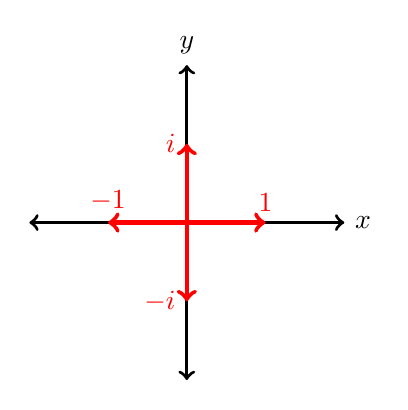
\begin{tikzpicture}
\draw[very thick, <->] (-2,0) -- (2,0) node[right] {$x$};
\draw[very thick, <->] (0,-2) -- (0,2) node[above] {$y$};
\draw[ultra thick, ->, red] (0,0) -- (1,0) node[above] {$1$};
\draw[ultra thick, ->, red] (0,0) -- (-1,0) node[above] {$-1$};
\draw[ultra thick, ->, red] (0,0) -- (0,1) node[left] {$i$};
\draw[ultra thick, ->, red] (0,0) -- (0,-1) node[ left] {$-i$};
\end{tikzpicture}
\end{center}
\end{Exam}

If $z= x+yi$ is a complex number, then its inverse $-z = -x-yi$ is graphed by the vector pointing in the opposite direction and same length. Its conjugate $\overline{z} = x-yi$ is graphed by the vector formed by reflecting $z$ across the real axis.
\begin{center}
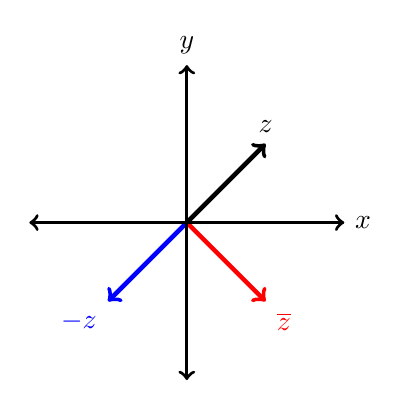
\begin{tikzpicture}
\draw[ultra thick, ->, blue] (0,0) -- (-1,-1) node[below left] {$-z$};
\draw[ultra thick, ->, red] (0,0) -- (1,-1) node[below right] {$\overline{z}$};
\draw[very thick, <->] (-2,0) -- (2,0) node[right] {$x$};
\draw[very thick, <->] (0,-2) -- (0,2) node[above] {$y$};
\draw[ultra thick, ->] (0,0) -- (1,1) node[above] {$z$};
\end{tikzpicture}
\end{center}

\begin{Def} The \textbf{absolute value} or \textbf{modulus} of the complex number $z=x+yi$ is the distance from the origin to the point $(x,y)$ in the complex plane. In other words, it is the magnitude of the vector $\bb z = \langle x,y\rangle$. If this distance is denoted by $r$, then 
\[r = |z| = |x+yi| = \sqrt{x^2+y^2}.\]
\end{Def}\vs

\begin{Exam} Find the modulus of each complex number: $5i$, $7$, and $3+4i$.
\begin{eqnarray*}
|5i| &=& \sqrt{0^2+5^2} = \sqrt{25} = \fbox{5}\\
|7| &=& \sqrt{7^2+0^2} = \sqrt{49} = \fbox{7}\\
|3+4i| &=& \sqrt{3^2+4^2} = \sqrt{9+16} = \sqrt{25} = \fbox{5}
\end{eqnarray*}
\end{Exam}\vs

\begin{Def} The \textbf{argument} of the complex number $z=x+yi$, denoted $\arg(z)$, is the smallest positive angle $\theta$ from the positive real axis to the graph of $z$. In other words, it is the direction of the vector $\bb z =\vr{x\\ y}$.
\end{Def}\vs

Note that $\arg(z) = \tan^{-1}\left(\dfrac{y}{x}\right) = \sin^{-1}\left(\dfrac{y}{|z|}\right) = \cos^{-1}\left(\dfrac{x}{|z|}\right)$.\\

Using basic trigonometry, we know that the components of $\bb z = \vr{x\\ y}$ are $x = r\cos \theta$ and $y=r\sin \theta$ where $r$ and $\theta$ are the magnitude and direction of $\bb z$, respectively. Therefore, for the complex number $z = x+yi$, if $r=|z|$ and $\theta=\arg(z)$, then 
\begin{eqnarray*}
z&=& x+yi = (r\cos\theta) + (r\sin\theta)i\\ 
&=& r\cos\theta + ri\sin\theta = r(\cos \theta + i\sin\theta)\footnotemark
\end{eqnarray*}

\begin{Def} Let $z=x+yi$, let $r=|z|$, and $\theta = \arg(z)$. Then 
\[z = r(\cos\theta + i\sin\theta)\] is the \textbf{polar form} of the complex number.
\end{Def}\vs

\begin{Thm}[Euler's Formula] Let $z=x+yi$, let $r=|z|$, and $\theta = \arg(z)$. Then
\[z = r(\cos\theta + i\sin\theta) = re^{i\theta}.\] In particular, 
\[e^{i\theta} = \cos\theta + i\sin\theta.\]
\end{Thm}
\begin{pf} It suffices to prove the second equation. To do so, remember the Taylor series of $e^x$, $\sin x$, and $\cos x$, which can be naturally extended to any complex number:
\begin{eqnarray*}
e^z &=& \dsum_{n=0}^\infty \dfrac{z^n}{n!} = 1+z+\dfrac{z^2}{2!} + \dfrac{z^3}{3!} + \dfrac{z^4}{4!} + \ldots\\
\sin(z) &=& \dsum_{n=0}^\infty (-1)^n\dfrac{z^{2n+1}}{(2n+1)!} = z-\dfrac{z^3}{3!} + \dfrac{z^5}{5!} - \dfrac{z^7}{7!} + \ldots\\ 
\cos(z) &=& \dsum_{n=0}^\infty (-1)^n\dfrac{z^{2n}}{(2n)!} = 1-\dfrac{z^2}{2!} + \dfrac{z^4}{4!} - \dfrac{z^6}{6!} + \ldots
\end{eqnarray*} The power series for $e^z$ then allows us to compute $e^{i\theta}$.
\begin{eqnarray*}
e^{i\theta} &=& \dsum_{n=0}^\infty \dfrac{{i\theta}^n}{n!} = 1+(i\theta)+\dfrac{(i\theta)^2}{2!} + \dfrac{(i\theta)^3}{3!} + \dfrac{(i\theta)^4}{4!} + \dfrac{(i\theta)^5}{5!} + \dfrac{(i\theta)^6}{6!} + \dfrac{(i\theta)^7}{7!}+ \ldots\\
&=& 1+i\theta-\dfrac{\theta^2}{2!} - \dfrac{i\theta^3}{3!} + \dfrac{\theta^4}{4!} + \dfrac{i\theta^5}{5!} - \dfrac{\theta^6}{6!} - \dfrac{i\theta^7}{7!}+ \ldots\\
&=& \left(1-\dfrac{\theta^2}{2!}+ \dfrac{\theta^4}{4!}- \dfrac{\theta^6}{6!} + \ldots\right) +\left(i\theta - \dfrac{i\theta^3}{3!}  + \dfrac{i\theta^5}{5!}  - \dfrac{i\theta^7}{7!}+ \ldots\right)\\
&=& \left(1-\dfrac{\theta^2}{2!}+ \dfrac{\theta^4}{4!}- \dfrac{\theta^6}{6!} + \ldots\right) +i\left(\theta - \dfrac{\theta^3}{3!}  + \dfrac{\theta^5}{5!}  - \dfrac{\theta^7}{7!}+ \ldots\right)\\
&=& \left(\dsum_{n=0}^\infty (-1)^n\dfrac{z^{2n}}{(2n)!}\right) +i\left(\dsum_{n=0}^\infty (-1)^n\dfrac{z^{2n+1}}{(2n+1)!}\right) = \cos(\theta) + i\sin(\theta)
\end{eqnarray*}
\end{pf}

When $\theta = \pi$, we get 
\[e^{\pi i} =  \cos\pi + i\sin\pi  = -1\]\vs

\begin{Exam} Write $z= -1+i$ in polar form.\\

Since $x=-1$ and $y=1$, $z$ will be in $Q2$. Also, we have $r = |z| = \sqrt{(-1)^2+1^2} = \sqrt{2}$. Likewise, $\theta = \arg(z) = \tan^{-1}\left(\dfrac{1}{-1}\right) = \tan^{-1} (-1) = \dfrac{3\pi}{4} (=135^\circ)$. Therefore, 
\[z = \fbox{$\sqrt{2}\left(\cos\left(\dfrac{3\pi}{4}\right) + i\sin\left(\dfrac{3\pi}{4}\right)\right) = \sqrt{2}e^{3\pi i/4}$}.\qedhere\]
\end{Exam}\vs

\begin{Exam} Write $z= 2e^{\pi i/3}$ in standard form.
\[z = 2e^{\pi i/3} = 2\left(\cos\left(\dfrac{\pi}{3}\right) + i\sin\left(\dfrac{\pi}{3}\right)\right) = 2\left(\dfrac{1}{2} + \dfrac{\sqrt{3}}{2}i\right) = \fbox{$1+i\sqrt{3}$}.\qedhere\]
\end{Exam}
 
 \vfill \footnotetext{Many trigonometry textbooks use the notation $\text{cis}\,\theta = \cos\theta + i\sin\theta$, which is not commonly used in advanced mathematics. For this reason, it would be better for you to not use $\text{cis}$. No cissing in class! Instead, use $e^{i\theta}$ to abbreviate $\cos\theta + i\sin\theta$.}
 


%%%% Magma %%%%%%  %%%%%%%%%%%% %%%%%% %%%%%% %%%%%% %%%%%% %%%%%% %%%%%% %%%%%% %%%%%% %%%%%%   
%%%%  %%%%%%  %%%%%%%%%%%% %%%%%% %%%%%% %%%%%% %%%%%% %%%%%% %%%%%% %%%%%% %%%%%% %%%%%%   
\chapter{MAGMA}\label{chap:magma}
In abstract algebra, like other mathematical disciplines, it can be very useful to have a ``calculator'' to assist with computations. Two computational algebra softwares appropriate for calculations in this book are MAGMA and GAP. Because MAGMA has a free, cloud based compiler, found at : \url{ http://magma.maths.usyd.edu.au/calc/}, we will utilize MAGMA code from time-to-time in this book. A detailed explanation for MAGMA can be found in its handbook: \url{http://magma.maths.usyd.edu.au/magma/handbook/}, but we can provide a few tips here. \\

In MAGMA, all commands must end with a semicolon \texttt{;} (line breaks are ignored completely. The special character \texttt{//} starts a comment in MAGMA. Any character in a line after \texttt{//} is ignored by the compiler and is used simply for notes for the programmer. Variables are declared with \texttt{:=}, for example, \texttt{ID := 1234;} MAGMA does not require you to cast your variable type. It is \emph{dynamic} in that the compilers learns what quantity based upon context. If $\circ$ is an operation, then \texttt{var $\circ$= num} replaces the current values of the variable \texttt{var} with \texttt{var $\circ$ num}.  For example, if \texttt{var := 3;}, then \texttt{var += 2;} changes the value of \texttt{var} from \texttt{3} to \texttt{5}.\\

 An array is started and ended with square brackets, \texttt{[} and \texttt{]}, and individual elements are separated by commas, or example, \texttt{[3,1,4,1,5,9]}. Arrays are lists, meaning they are ordered and repetition is allowed. The array $[1,2,\ldots, n]$ can quickly be produced as \texttt{[1..n]}. The special character \# gives the number of elements in an array. For example, If \texttt{array} is an array, then \texttt{\#array} returns the number of elements in \texttt{array}.  Referencing the $i$th element of \texttt{array} is done as \texttt{array[i]}. If the $i$th element of \texttt{array} is itself an array, then the $j$th element of \texttt{array[i]} is received as \texttt{array[i,j]}.  If \texttt{array1} and \texttt{array2} are two arrays, then \texttt{array1 cat array2} is the concatenation of the two arrays, putting \texttt{array1} first, followed immediately by \texttt{array2}. For example, \texttt{[1,2,3] cat [4,5];} return \texttt{[1,2,3,4,5]}.  For an associative operation $\circ$, e.g. $+$, $*$, \texttt{cat}, then \texttt{\&+ $\circ$} computes the \texttt{\#array}-fold $\circ$-product \texttt{array}. For example, \texttt{\&+array} computes the sum of \texttt{array}.\\

\begin{Exam*}
One can print to screen simply by stating the variable or quantity you want. For example, 
\begin{lstlisting}[language=Magma]
p := 37316150861565913091; 
q := 62369111002657007863; // This is a comment.
n := p*q; n;
\end{lstlisting} returns \texttt{2327375155276899373645006956575561634533}, the product of two large primes.
\end{Exam*}\vs

\begin{Exam*} To compute $\gcd(a,b)$ for $a,b\in \Z$ in MAGMA, type \texttt{Gcd(a,b);}. This will execute an algorithm similar to the Euclidean algorithm given in \examref{exam:euclideanalg}. For example, \texttt{Gcd(6,561);} returns \texttt{3}.
\end{Exam*}\vs

\begin{Exam*} To compute $a^{-1}\pmod n$ for $a,b\in \Z$ and $\gcd(a,n)$ in MAGMA, type \texttt{InverseMod(a,n);}. This will execute an algorithm similar to the Euclidean algorithm given in \examref{exam:euclideanalg}. For example, \texttt{InverseMod(629,3432);} returns \texttt{1997}.
\end{Exam*}\vs

\begin{Exam*}\label{exam:magma:modexp} To compute $a^m \pmod n$ for $a,m,n\in \Z$ in MAGMA, type \texttt{Modexp(a,m,n);}. This will execute an algorithm similar to the Repeated Squares algorithm given in \examref{exam:repeatedsquares}. For example, \texttt{Modexp(2,560,561);} returns \texttt{1}.\\

Alternatively, one could use \verb+(a^m) mod n;+, but, unfortunately, this command will compute $a^m$ first in $\Z$ then reduce modulo $n$ which can lead to runtime errors if $a^m$ is too large. The command \texttt{Modexp} instead runs the repeated squares algorithm which is much faster and not prone to error.
\end{Exam*}\vs

\begin{Exam*} To factor an integer $n\in \Z$ in MAGMA, type \texttt{Factorization(n);}. This will produce a factorization of $n$ as a list of pairs \texttt{<p,k>}, where $p$ is a prime factor of $n$ and $k$ is the largest power of $p$ which divides $n$. Hence, $p^k\mid n$ but $p^{k+1}\nmid n$. For example, \texttt{Factorization(67989839287140);} returns \texttt{[ <2, 2>, <3, 4>, <5, 1>, <19, 1>, <109, 1>, <2287, 1>, <8861, 1> ]}, since 
\[67989839287140 = 2^2\cdot 3^4\cdot 5\cdot 19\cdot 109\cdot 2287\cdot 8861.\]

To access specific pairs within the factorization, say \texttt{fact := Factorization(67989839287140);}, call an entry of the array by concatenating \texttt{[i]} at the end of the array. For example, \texttt{fact[2];} return \texttt{<3,4>}. If you want a specific prime or exponent in this factorization, use a double index \texttt{[i,j]}. For example, \texttt{fact[2,1];} return \texttt{3}. Note that we can compute the product of any $n$ by \verb+&*[fact[i,1]^fact[i,2] : i in [1..#fact]];+, where \texttt{fact := Factorization(n);}.\\

Like in \secref{RSA}, imagine that Eve find Bob's RSA public key $(n,e)$. In order to decrypt messages sent to Bob from Alice, Eve needs to compute Bob's private key $d$, which is the solution to the congruence $de \equiv 1 \pmod{\phi(n)}$. She knows that $n=pq$ is a semiprime, that is, $p$ and $q$ are primes. As $n$ is not very large, she is able to factor $n$, revealing $p$ and $q$. With this factorization, Eve can easily compute $\phi(n) = \phi(p)\phi(q) = (p-1)(q-1)$. The following code finds Bob's private key:
\begin{lstlisting}[language=Magma]
n := 3551; e := 629;

fact := Factorization(n); 
p:=fact[1,1]; q:=fact[2,1];

phi := (p-1)*(q-1);
d := InverseMod(e,phi); d;
\end{lstlisting}
which returns \texttt{1997}. Hence, the protection RSA comes down to how efficient \texttt{Factorization} runs. The general strategy to avoid factorization of $n$ is to use BIG primes $p$ and $q$, so that even the best factoring algorithms cannot find it in a short  amount of time.
\end{Exam*}\vs

\begin{Exam*} Continuing the previous example, how does one find BIG primes? Given any integer $n$, MAGMA can find the next prime after $n$ with the command \texttt{NextPrime(n);} (there is a similar function \texttt{PreviousPrime}.\footnotemark\ For example, the command \texttt{NextPrime(67989839287140);} returns \texttt{67989839287147} (if every you are not sure if a number $n$ is prime or not, run \texttt{IsPrime(n);}, which returns \texttt{True} if $n$ is prime and \texttt{False} otherwise). \\

Another useful MAGMA function is \texttt{Random(a,b);} which computes a random integer between $a,b\in\Z$. For example, \texttt{Random(629,1997);} may return \texttt{1626} or \texttt{1373} or \texttt{1200}, since each run will produce a random value (if you are using random numbers, make sure to record them before your next compile). Combining this with \texttt{NextPrime}, we can create a random prime generator, where \texttt{NextPrime(Random(a,b));} returns a random prime between $a$ and $b$. For example,  \texttt{NextPrime(Random(10\textasciicircum10,10\textasciicircum20));} may return \texttt{37316150861565913091} or \texttt{62369111002657007863}, which are two primes between 10 and 20 digits long. Such a strategy could be useful in generating keys for RSA.
\end{Exam*}\vs

\footnotetext{Because of primality tests, some of which are hinted toward in the Exercises of \secref{lagrange}, we can find primes easy enough, but factoring is still hard.}

\chapter{Solutions to Select Exercises}\label{apx:solutions}

%%%%%%%%%%%% %%%%%% %%%%%% %%%%%% %%%%%% %%%%%% %%%%%% %%%%%% %%%%%% %%%%%%   
%%%%%%%%%%%% %%%%%% %%%%%% %%%%%% %%%%%% %%%%%% %%%%%% %%%%%% %%%%%% %%%%%%   
%%%% Solutions %%%%%%%%%%%% %%%%%% %%%%%% %%%%%% %%%%%% %%%%%% %%%%%% %%%%%% %%%%%% %%%%%%    
%%%%%%%%%%%% %%%%%% %%%%%% %%%%%% %%%%%% %%%%%% %%%%%% %%%%%% %%%%%% %%%%%%   
%%%%%%%%%%%% %%%%%% %%%%%% %%%%%% %%%%%% %%%%%% %%%%%% %%%%%% %%%%%% %%%%%%  
\startSolutionsChap{Abstract Prealgebra}{prealgebra}
%%%% Section 1.1 %%%%%%  %%%%%%%%%%%% %%%%%% %%%%%% %%%%%% %%%%%% %%%%%% %%%%%% %%%%%% %%%%%% %%%%%%   
%%%%  %%%%%%  %%%%%%%%%%%% %%%%%% %%%%%% %%%%%% %%%%%% %%%%%% %%%%%% %%%%%% %%%%%% %%%%%%   
\startSolutions{Sets}{sets}
\begin{enumerate}[!HW!]
\begin{multicols}{2}
\item $\{2\}$
\item $\{5\}$
\end{multicols}
\end{enumerate}
\vspace{-15pt}
%%%% Section 1.2 %%%%%%  %%%%%%%%%%%% %%%%%% %%%%%% %%%%%% %%%%%% %%%%%% %%%%%% %%%%%% %%%%%% %%%%%%   
%%%%  %%%%%%  %%%%%%%%%%%% %%%%%% %%%%%% %%%%%% %%%%%% %%%%%% %%%%%% %%%%%% %%%%%% %%%%%%   
\startSolutions{Functions}{function}
\begin{enumerate}[!HW!]
\columnratio{0.75}
\begin{paracol}{2}
\item $\{(a,1),(a,2),(a,3),(b,1),(b,2),(b,3),(c,1),(c,2),(c,3)\}$
\switchcolumn
\setcounter{enumi}{\getrefnumber{exer:cartesianproduct:stop}-1}
\item $\emptyset$
\end{paracol}
\begin{multicols}{4}
\setcounter{enumi}{\getrefnumber{exer:welldefined:start}-1}
\item Not function
\item Function
\item Not function
\item Function
\end{multicols}
\begin{multicols}{2}
\item One-to-one, not onto
\item Not one-to-one, not onto
\end{multicols}
\begin{multicols}{2}
\item Not one-to-one, not onto
\item Not one-to-one, onto
\end{multicols}
\end{enumerate}
\vspace{-15pt}

%%%% Section 1.3 %%%%%%  %%%%%%%%%%%% %%%%%% %%%%%% %%%%%% %%%%%% %%%%%% %%%%%% %%%%%% %%%%%% %%%%%%   
%%%%  %%%%%%  %%%%%%%%%%%% %%%%%% %%%%%% %%%%%% %%%%%% %%%%%% %%%%%% %%%%%% %%%%%% %%%%%%   
\startSolutions{Inverse Functions and Permutations}{inverse}
\begin{enumerate}[!HW!, start=\getrefnumber{exer:inversefunction}]
\item $\dom f = \im f= (-\infty,1)\cup (1,\infty)$, $f^{-1}(x) =\dfrac{x+1}{x-1}$, $(f\circ f^{-1})(x) = (f^{-1}\circ f)(x) = x$
\end{enumerate}
\vspace{-15pt}

%%%% Section 1.4 %%%%%%  %%%%%%%%%%%% %%%%%% %%%%%% %%%%%% %%%%%% %%%%%% %%%%%% %%%%%% %%%%%% %%%%%%   
%%%%  %%%%%%  %%%%%%%%%%%% %%%%%% %%%%%% %%%%%% %%%%%% %%%%%% %%%%%% %%%%%% %%%%%% %%%%%%   
\startSolutions{Equivalence Classes}{equivalence}
\begin{enumerate}[!HW!, start=\getrefnumber{exer:equivalence:start}]
\begin{multicols}{3}
\item Not symmetric
\item Not transitive
\item Not reflexive
\end{multicols}
\begin{multicols}{2}
\item Equivalence relation
\item Not symmetric
\end{multicols}
\begin{multicols}{2}
\item Equivalence relation
\item Equivalence relation
\end{multicols}
\end{enumerate}
\vspace{-15pt}


%%%% Section 1.5 %%%%%%  %%%%%%%%%%%% %%%%%% %%%%%% %%%%%% %%%%%% %%%%%% %%%%%% %%%%%% %%%%%% %%%%%%   
%%%%  %%%%%%  %%%%%%%%%%%% %%%%%% %%%%%% %%%%%% %%%%%% %%%%%% %%%%%% %%%%%% %%%%%% %%%%%%   
\startSolutions{Induction and the Well--Ordering Principle}{induction}
\begin{enumerate}[!HW!, start=\getrefnumber{exer:induction:stop}]
\item \emph{\color{magenta} For the inductive step where $|X| = n+1$, let $x\in X$ be some distinguished element. If $A\subseteq X$, then $A\setminus \{x\} \subseteq X\setminus \{x\}$. How many options are there for $A\setminus \{x\}$ then? Either $x\in A$ or $x\notin A$, which gives two options independent of the previous number.}
\end{enumerate}
\vspace{-15pt}


%%%% Section 1.6 %%%%%%  %%%%%%%%%%%% %%%%%% %%%%%% %%%%%% %%%%%% %%%%%% %%%%%% %%%%%% %%%%%% %%%%%%   
%%%%  %%%%%%  %%%%%%%%%%%% %%%%%% %%%%%% %%%%%% %%%%%% %%%%%% %%%%%% %%%%%% %%%%%% %%%%%%   
\startSolutions{Divisibility of Integers}{integers}

\begin{enumerate}[!HW!]
\begin{multicols}{3}
\item  $1 = 14(14) - 5(39)$
\item  $3 = -17(165) + 12(234)$
\item  $1 = 3709(1739) - 650(9923)$
\end{multicols}
\begin{multicols}{3}
\item  $1 = -105(471) + 88(562)$
\item  \scalebox{0.99}{$1 = -1050(19945) + 881(23771)$}
\item  $1 = 1463(-4357) + 1698(3754)$
\end{multicols}
\setcounter{enumi}{\getrefnumber{exer:lcm}-1}
\item \emph{\color{magenta} Use the Well-Ordering Principle combined with the Division Algorithm.}
\setcounter{enumi}{\getrefnumber{exer:integers:stop}-1}
\item \emph{\color{magenta} $ar+bs=1$ implies that $arc+bsc = c$.}
\end{enumerate}
\vspace{-15 pt}

%%%% Supplementary Exercises %%%%%%  %%%%%%%%%%%% %%%%%% %%%%%% %%%%%% %%%%%% %%%%%% %%%%%% %%%%%% %%%%%% %%%%%%   
%%%%  %%%%%%  %%%%%%%%%%%% %%%%%% %%%%%% %%%%%% %%%%%% %%%%%% %%%%%% %%%%%% %%%%%% %%%%%%   
\startSuppSolutions{prealgebra}

\begin{enumerate}[!HW!, start=\getrefnumber{exer:primesquare}]
\item  \emph{\color{magenta} Use the Fundamental Theorem of Arithmetic.}
\setcounter{enumi}{\getrefnumber{exer:infiniteprimesixfive}-1}
\item \emph{\color{magenta} Every prime has the form $2, 3, 6n+1$, or $6n+5$. }
\setcounter{enumi}{\getrefnumber{exer:irrational2}-1}
\item \emph{\color{magenta} Prove by contradiction. If not, $\sqrt{2}=\dfrac{p}{q}$ for some $p,q\in \Z$ and $\gcd(p,q)=1$. Show that $p^2=2q^2$. Apply Euclid's Lemma.}
\end{enumerate}
\vspace{-15 pt}

%%%%%%%%%%%% %%%%%% %%%%%% %%%%%% %%%%%% %%%%%% %%%%%% %%%%%% %%%%%% %%%%%%   
%%%%%%%%%%%% %%%%%% %%%%%% %%%%%% %%%%%% %%%%%% %%%%%% %%%%%% %%%%%% %%%%%%  
\startSolutionsChap{Group Theory}{group}
%%%% Section 2.1 %%%%%%  %%%%%%%%%%%% %%%%%% %%%%%% %%%%%% %%%%%% %%%%%% %%%%%% %%%%%% %%%%%% %%%%%%   
%%%%  %%%%%%  %%%%%%%%%%%% %%%%%% %%%%%% %%%%%% %%%%%% %%%%%% %%%%%% %%%%%% %%%%%% %%%%%%   
\startSolutions{Groups}{group}
\begin{enumerate}[!HW!]
\begin{multicols}{6}
\item $x\equiv 3$
\item $x\equiv 7$
\item $x\equiv 18$
\item $x\equiv 2$
\item $x\equiv 5$
\item $\emptyset$
\end{multicols}
\setcounter{enumi}{\getrefnumber{exer:modularproof:start}-1} 
\item \emph{\color{magenta} Show that the operations do not depend on the choice of the representative from the equivalence classes modulo $n$.}
\end{enumerate}
\vspace{-15pt}

%%%% Section 2.2 %%%%%%  %%%%%%%%%%%% %%%%%% %%%%%% %%%%%% %%%%%% %%%%%% %%%%%% %%%%%% %%%%%% %%%%%%   
%%%%  %%%%%%  %%%%%%%%%%%% %%%%%% %%%%%% %%%%%% %%%%%% %%%%%% %%%%%% %%%%%% %%%%%% %%%%%%   
\startSolutions{Cayley Tables}{cayley}
\begin{enumerate}[!HW!]
\begin{multicols}{4}
\item Not group
\item Group
\item Group
\item Not Group
\end{multicols}
\setcounter{enumi}{\getrefnumber{exer:cayleycounter:start}-1} 
\item \emph{\color{magenta} There is a nonabelian group containing six elements.}
\item \emph{\color{magenta} The are five different groups of order 8.}
\end{enumerate}
\vspace{-15pt}


%%%% Section 2.3 %%%%%%  %%%%%%%%%%%% %%%%%% %%%%%% %%%%%% %%%%%% %%%%%% %%%%%% %%%%%% %%%%%% %%%%%%   
%%%%  %%%%%%  %%%%%%%%%%%% %%%%%% %%%%%% %%%%%% %%%%%% %%%%%% %%%%%% %%%%%% %%%%%% %%%%%%   
\startSolutions{Properties of Groups}{groupprop}
\begin{enumerate}[!HW!, start=\getrefnumber{exer:groupprop:pickstart}]
\item \emph{\color{magenta} Since $abab=(ab)^2=e=a^2b^2=aabb$, use Cancellation.}
\setcounter{enumi}{\getrefnumber{exer:a4b=ba}-1}
\item \emph{\color{magenta} $a^4b=a^3(ab)$}
\end{enumerate}
\vspace{-15pt}

%%%% Section 2.4 %%%%%%  %%%%%%%%%%%% %%%%%% %%%%%% %%%%%% %%%%%% %%%%%% %%%%%% %%%%%% %%%%%% %%%%%%   
%%%%  %%%%%%  %%%%%%%%%%%% %%%%%% %%%%%% %%%%%% %%%%%% %%%%%% %%%%%% %%%%%% %%%%%% %%%%%%   
\startSolutions{Subgroups}{subgroup}
\begin{enumerate}[!HW!, start=\getrefnumber{exer:subgroup:quadratic}]
\item \emph{\color{magenta} The identity of $H$ is $1=1+0\sqrt{2}$. Show that  $(a+b\sqrt{2})(c+d\sqrt{2}) = (ad+bc)+(ad+bc)\sqrt{2}$ and $(a+b\sqrt{2})^{-1}=\dfrac{a}{a^2-2b^2}- \dfrac{b}{a^2-2b^2}\sqrt{2}$.}
\setcounter{enumi}{\getrefnumber{exer:subgroup:union}-1} 
\item \emph{\color{magenta} Look at $S_3$.}
\end{enumerate}
\vspace{-15pt}

%%%% Section 2.5 %%%%%%  %%%%%%%%%%%% %%%%%% %%%%%% %%%%%% %%%%%% %%%%%% %%%%%% %%%%%% %%%%%% %%%%%%   
%%%%  %%%%%%  %%%%%%%%%%%% %%%%%% %%%%%% %%%%%% %%%%%% %%%%%% %%%%%% %%%%%% %%%%%% %%%%%%   
\startSolutions{Hasse Diagrams}{hasse}
\begin{enumerate}[!HW!, start=\getrefnumber{exer:poset:D3}]
\item \emph{\color{magenta} $S_3$ has five subgroups: $H_1=\{id\}, H_2=\{id, \rho_1, \rho_2\}, H_3=\{id, \sigma_1\}, H_4=\{id, \sigma_2\}, S_3$.}
\end{enumerate}
\vspace{-15pt}

%%%% Section 2.6 %%%%%%  %%%%%%%%%%%% %%%%%% %%%%%% %%%%%% %%%%%% %%%%%% %%%%%% %%%%%% %%%%%% %%%%%%   
%%%%  %%%%%%  %%%%%%%%%%%% %%%%%% %%%%%% %%%%%% %%%%%% %%%%%% %%%%%% %%%%%% %%%%%% %%%%%%   
\startSuppSolutions{group}
\begin{enumerate}[!HW!, start=\getrefnumber{exer:group:noncommutematrix}]
\item \emph{\color{magenta} Pick any two matrices and you probably have what you need.}
\setcounter{enumi}{\getrefnumber{exer:group:noncommutedihedral}-1}
\item \emph{\color{magenta} The group will have to be nonabelian and $n\ge 2$. So maybe try $D_4$.}

\setcounter{enumi}{\getrefnumber{exer:group:commutatorpower}-1}
\item \emph{\color{magenta} $(ghg^{-1})^n = (ghg^{-1})(ghg^{-1})\cdots(ghg^{-1}) = gh(g^{-1}g)h(g^{-1}g)\cdots (g^{-1}g)hg^{-1}$}
\item \emph{\color{magenta} Prove that the number of elements whose order is not 2 must be odd}
\end{enumerate}
\vspace{-15pt}


%%%%%%%%%%%% %%%%%% %%%%%% %%%%%% %%%%%% %%%%%% %%%%%% %%%%%% %%%%%% %%%%%%   
%%%%%%%%%%%% %%%%%% %%%%%% %%%%%% %%%%%% %%%%%% %%%%%% %%%%%% %%%%%% %%%%%%  
\startSolutionsChap{Cyclic Groups}{cyclic}
%%%% Section 3.1 %%%%%%  %%%%%%%%%%%% %%%%%% %%%%%% %%%%%% %%%%%% %%%%%% %%%%%% %%%%%% %%%%%% %%%%%%   
%%%%  %%%%%%  %%%%%%%%%%%% %%%%%% %%%%%% %%%%%% %%%%%% %%%%%% %%%%%% %%%%%% %%%%%% %%%%%%   
\startSolutions{Cyclic Groups}{cyclic}
\begin{enumerate}[!HW!]
\begin{multicols}{6}
\item 12
\item $\infty$
\item $\infty$ 
\item 4
\item 10
\item 157
\end{multicols}
\end{enumerate}
\vspace{-15pt}

%%%% Section 3.2 %%%%%%  %%%%%%%%%%%% %%%%%% %%%%%% %%%%%% %%%%%% %%%%%% %%%%%% %%%%%% %%%%%% %%%%%%   
%%%%  %%%%%%  %%%%%%%%%%%% %%%%%% %%%%%% %%%%%% %%%%%% %%%%%% %%%%%% %%%%%% %%%%%% %%%%%%   
\startSolutions{Roots of Unity}{rootunity}
\begin{enumerate}[!HW!]
\begin{multicols}{6}
\item $\sqrt(3)+i$
\item $\dfrac{5\sqrt{2}}{2} + \dfrac{5\sqrt{2}}{2}i$
\item $-3$
\item $\dfrac{\sqrt{2}}{4}-\dfrac{\sqrt{2}}{4}i$

\item $\sqrt{2}e^{7\pi i/4}$
\item $5e^{\pi i}$
\item $2\sqrt{2}e^{\pi i /4}$
\item  $2e^{\pi i/6}$
\item $3e^{3\pi i/2}$
\item $4e^{\pi i/3}$

\item 15
\item $-3+3i$
\item $8-i$
\item $43-18i$
\item 82
\item $i$
\item 2


\item $\infty$
\item $\infty$ 
\item 4
\item 10
\item 157

\item $\dfrac{1}{2}-\frac{i}{2}$
\item $8i$
\item $-16\sqrt{3}+16i$
\item $-1$
\item $-\dfrac{1}{4}$
\item $-4096$
\item $\dfrac{1}{256}+\dfrac{i}{256}$
\end{multicols}
\end{enumerate}
\vspace{-15pt}


%%%% Section 3.3 %%%%%%  %%%%%%%%%%%% %%%%%% %%%%%% %%%%%% %%%%%% %%%%%% %%%%%% %%%%%% %%%%%% %%%%%%   
%%%%  %%%%%%  %%%%%%%%%%%% %%%%%% %%%%%% %%%%%% %%%%%% %%%%%% %%%%%% %%%%%% %%%%%% %%%%%%   
\startSolutions{Orders of Group Elements}{repeated}

\begin{enumerate}[!HW!]
\begin{multicols}{2}
\item$7\Z = \{\ldots, -7,0,7,14,\ldots\}$
\item $\langle 15\rangle = \{0,3,6,9,12,15,18,21\} = 3\Z_{24}$
\end{multicols}
\begin{multicols}{2}
\item $\langle 8\rangle = \{0,4,8\} = 4\Z_{12}$
\item $\langle 8\rangle = \{0,4,8,12,16,20,24,28,32,36,40,44,48,52,56\} = 4\Z_{60}$ 
\end{multicols}
\begin{multicols}{2}
\item $\langle 8\rangle = \{0,1,2,3,4,5,6,7,8,9,10,11,12\} = \Z_{13}$
\item $\langle 8\rangle = \{0,8,16,24,32,40\} = 8\Z_{48}$  
\end{multicols}
\begin{multicols}{2}
\item $\langle 3\rangle = \{1,3,7,9\}$
\item $\langle 5\rangle = \{1, 5, 7, 11, 13, 17\} = \Z_{18}^*$
\end{multicols}
\begin{multicols}{2}
\item $\langle 7\rangle = \left\{\ldots, \dfrac{1}{49}, \dfrac{1}{7},1,7,49,343\ldots\right\}$
\item $\langle i\rangle = \langle i\rangle = \{1,-1,i,-i\}$
\end{multicols}
\begin{multicols}{2}
\item $\langle 2i\rangle = \left\{\ldots, -\dfrac{1}{4}, -\dfrac{i}{2},1,2i,-4,-8i, 16\ldots\right\}$
\item $\langle e^{\pi i /4}\rangle = \left\{\pm 1, \pm i, \pm\dfrac{\sqrt{2}}{2}\pm\dfrac{\sqrt{2}}{2}i\right\}$
\end{multicols}
\item $\langle e^{\pi i/6}\rangle =   \left\{\pm 1, \pm i, \pm\dfrac{1}{2}\pm\dfrac{\sqrt{3}}{2}i, \pm\dfrac{\sqrt{3}}{2}\pm\dfrac{1}{2}i\right\}$

\setcounter{enumi}{\getrefnumber{exer:repeatedsquare:start}-1}
\begin{multicols}{4}
\item 292
\item  2876
\item 1523
\item 206
\end{multicols}
\end{enumerate}

%%%% Section 3.4 %%%%%%  %%%%%%%%%%%% %%%%%% %%%%%% %%%%%% %%%%%% %%%%%% %%%%%% %%%%%% %%%%%% %%%%%%   
%%%%  %%%%%%  %%%%%%%%%%%% %%%%%% %%%%%% %%%%%% %%%%%% %%%%%% %%%%%% %%%%%% %%%%%% %%%%%%   
\startSuppSolutions{cyclic}
\begin{enumerate}[!HW!, start=\getrefnumber{exer:cyclicdisprove:start}]
\begin{multicols}{3}
\item {\color{magenta} False}
\setcounter{enumi}{\getrefnumber{exer:cyclicdisprove:middle}-1}
\item {\color{magenta} False}
\setcounter{enumi}{\getrefnumber{exer:cyclicdisprove:stop}-1}
\item {\color{magenta} True}
\end{multicols}
\begin{multicols}{3}
\item $\{0\}$, $\{1,-1\}$, $\{1,-1\}$
\item 1,2,3,4,6,8,12,24
\item 240
\end{multicols}
\end{enumerate}
\vspace{-15pt}

%%%%%%%%%%%% %%%%%% %%%%%% %%%%%% %%%%%% %%%%%% %%%%%% %%%%%% %%%%%% %%%%%%   
%%%%%%%%%%%% %%%%%% %%%%%% %%%%%% %%%%%% %%%%%% %%%%%% %%%%%% %%%%%% %%%%%%  
\startSolutionsChap{Permutation Groups}{permutation}
%%%% Section 4.1 %%%%%%  %%%%%%%%%%%% %%%%%% %%%%%% %%%%%% %%%%%% %%%%%% %%%%%% %%%%%% %%%%%% %%%%%%   
%%%%  %%%%%%  %%%%%%%%%%%% %%%%%% %%%%%% %%%%%% %%%%%% %%%%%% %%%%%% %%%%%% %%%%%% %%%%%%   
\startSolutions{The Symmetric Group}{permutation}

\begin{enumerate}[!HW!]
\begin{multicols}{6}
\item $(12453)$
\item  $(14)(35)$
\item  $(13)(25)$
\item $(1325)$
\item $(135)(24)$
\item  $(253)$
\end{multicols}
\begin{multicols}{6}
\item  $(14)(23)$
\item $(12)(56)$
\item $(1324)$
\item $(13254)$
\item $(134)(25)$
\item $(14)(235)$
\end{multicols}
\begin{multicols}{6}
\item $(143)(25)$
\item 1
\item 4
\item 2
\item $(12)$
\item $(17352)$
\end{multicols}
\begin{multicols}{3}
\item $(1532)(476)$
\item \emph{\color{magenta} Show first that $\sigma\tau\sigma^{-1}(\sigma(a_i)) = \sigma(a_{i+1})$.}
\end{multicols}
\end{enumerate}
\vspace{-15pt}

%%%% Section 4.2 %%%%%%  %%%%%%%%%%%% %%%%%% %%%%%% %%%%%% %%%%%% %%%%%% %%%%%% %%%%%% %%%%%% %%%%%%   
%%%%  %%%%%%  %%%%%%%%%%%% %%%%%% %%%%%% %%%%%% %%%%%% %%%%%% %%%%%% %%%%%% %%%%%% %%%%%%   
\startSolutions{The Alternating Group}{transposition}

\begin{enumerate}[!HW!]
\begin{multicols}{3}
\item $(14)(43)(35)(56)$\\ even
\item $(15)(56)(23)(34)$\\ even
\item $(16)(14)(12) = (12)(24)(46)= (16)(12)(14)(12)(14)$\\ odd 
\end{multicols}

\item $(12)(17)(16)(14) = (14)(46)(67)(72) = (14)(15)(12)(17)(13)(12)(14)(12)(13)(16)(14)(15)$ \\ even 
\item $(14)(42)(26)(63)(37)$ odd

\item $A_5: 1, (12)(34), (123), (12345)$; $A_6: 1, (12)(34), (12)(3456), (123), (123)(456), (12345)$

\begin{multicols}{3}
\setcounter{enumi}{\getrefnumber{exer:transpositioncompute:stop}-2}
\item No, $26$ does not divide $\dfrac{8!}{2}$.
\item \emph{\color{magenta}$(1,2,3,4)(5,6,7,8,9,10)$}
\setcounter{enumi}{\getrefnumber{exer:transpositionproof:stop}}
\item \emph{\color{magenta} $(abc)=(ac)(ab)$}
\end{multicols}
\end{enumerate}
\vspace{-15pt}

%%%% Section 4.3 %%%%%%  %%%%%%%%%%%% %%%%%% %%%%%% %%%%%% %%%%%% %%%%%% %%%%%% %%%%%% %%%%%% %%%%%%   
%%%%  %%%%%%  %%%%%%%%%%%% %%%%%% %%%%%% %%%%%% %%%%%% %%%%%% %%%%%% %%%%%% %%%%%% %%%%%%   
\startSolutions{The Dihedral Group}{dihedral}

\begin{enumerate}[!HW!]
\item \emph{\color{magenta} $r=(12345),  s=(25)(34)$}

\setcounter{enumi}{\getrefnumber{exer:symmetrygroupfirst:stop}-1}
\begin{multicols}{5}
\item $D_4$
\item $D_2\cong V_4$
\item $Z_4$
\item $Z_2$
\item $Z_1\cong 1$
\end{multicols}
\begin{multicols}{5}
%\item  $S^1$
\item  $D_4$
\item $D_4$
\item $D_4$
\item $D_1\cong Z_2$
\end{multicols}
\end{enumerate}
\vspace{-15pt}

%%%% Section 4.4 %%%%%%  %%%%%%%%%%%% %%%%%% %%%%%% %%%%%% %%%%%% %%%%%% %%%%%% %%%%%% %%%%%% %%%%%%   
%%%%  %%%%%%  %%%%%%%%%%%% %%%%%% %%%%%% %%%%%% %%%%%% %%%%%% %%%%%% %%%%%% %%%%%% %%%%%%   
\startSuppSolutions{permutation}
\begin{enumerate}[!HW!]
\begin{multicols}{2}
\item $(a_1a_2\ldots a_n)^{-1} = (a_n\ldots a_2a_1)$
\item $\{(13), (13)(24), (132), (134), (1324), (1342)\}$,\\ not subgroup
\end{multicols}
\setcounter{enumi}{\getrefnumber{exer:permsuppS4:start}-1}
\begin{multicols}{2}
\item $\{1, (13), (14), (34), (134), (143)\}$,\\ subgroup 
\item $\{1, (13), (134)\}$, not subgroup 
\end{multicols}

\setcounter{enumi}{\getrefnumber{exer:snnonabelian}-1}
\item \emph{\color{magenta} $(123)(12) \neq (12)(123)$}

\setcounter{enumi}{\getrefnumber{exer:symmetrycube}-1}
\item {\color{magenta} Consider how rigid motions in $\R^3$ affect the four diagonals of the cube.}
\end{enumerate}
\vspace{-15pt}


%%%%%%%%%%%% %%%%%% %%%%%% %%%%%% %%%%%% %%%%%% %%%%%% %%%%%% %%%%%% %%%%%%   
%%%%%%%%%%%% %%%%%% %%%%%% %%%%%% %%%%%% %%%%%% %%%%%% %%%%%% %%%%%% %%%%%%  
\startSolutionsChap{Cosets}{cosets}
%%%% Section 5.1 %%%%%%  %%%%%%%%%%%% %%%%%% %%%%%% %%%%%% %%%%%% %%%%%% %%%%%% %%%%%% %%%%%% %%%%%%   
%%%%  %%%%%%  %%%%%%%%%%%% %%%%%% %%%%%% %%%%%% %%%%%% %%%%%% %%%%%% %%%%%% %%%%%% %%%%%%   
\startSolutions{Cosets}{cosets}

\begin{enumerate}[!HW!]
\item $\langle 8\rangle, 1+\langle 8\rangle, 2+\langle 8\rangle, 3+\langle 8\rangle, 4+\langle 8\rangle, 5+\langle 8\rangle, 6+\langle 8\rangle, 7+\langle 8\rangle$
\begin{multicols}{3}
\item $\langle 3\rangle, 5\langle 3\rangle$
\item $3\Z, 1+3\Z, 2+3\Z$
\item $A_4, (12)A_4$
\end{multicols}
\begin{multicols}{3}
\item $A_n, (12)A_n$
\item $D_4, (12)D_4, (14)D_4$
\item all circles centered at the origin
\end{multicols}
\item $\langle (123)\rangle, (12)\langle (123)\rangle, (14)\langle (123)\rangle, (24)\langle (123)\rangle, (34)\langle (123)\rangle, (12)(34)\langle (123)\rangle, (13)(24)\langle (123)\rangle, (14)(23)\langle (123)\rangle$

\begin{multicols}{2}
\item \emph{\color{magenta}  It is not well-defined.}
\item \emph{\color{magenta} If $gh\in gH$, then $gh=(ghg^{-1})g$ and $ghg^{-1}\in H$.}
\end{multicols}
\item \emph{\color{magenta} Show that $g(H\cap K) = gH\cap gK$.}
\end{enumerate}
\vspace{-15pt}

%%%% Section 5.2 %%%%%%  %%%%%%%%%%%% %%%%%% %%%%%% %%%%%% %%%%%% %%%%%% %%%%%% %%%%%% %%%%%% %%%%%%   
%%%%  %%%%%%  %%%%%%%%%%%% %%%%%% %%%%%% %%%%%% %%%%%% %%%%%% %%%%%% %%%%%% %%%%%% %%%%%%   
\startSolutions{Lagrange's Theorem}{lagrange}

\begin{enumerate}[!HW!]
\begin{multicols}{3}
\item 1, 2, 3, 4, 5, 6, 10,\\ 12, 15, 20, 30, 60
\item \emph{\color{magenta} $|g|, |h| \mid |G|$}
\item \emph{\color{magenta} Use Fermat's Little Theorem.}
\end{multicols}

\setcounter{enumi}{\getrefnumber{exer:pseudoprime:start}-1}
\begin{multicols}{3}
\item 86, certainly composite 
\item 1 maybe prime
\item 1, maybe prime
\end{multicols}
\begin{multicols}{3}
\item 1, maybe prime
\item 4, certainly composite
\item 1, maybe prime
\end{multicols}
\begin{multicols}{3}
\item 279, certainly composite 
\item 1 maybe prime
\item 1, maybe prime
\end{multicols}
\begin{multicols}{3}
\item 375, certainly composite
\item 9, certainly composite
\item 1, maybe prime
\end{multicols}
\end{enumerate}
\vspace{-15pt}

%%%% Section 5.3 %%%%%%  %%%%%%%%%%%% %%%%%% %%%%%% %%%%%% %%%%%% %%%%%% %%%%%% %%%%%% %%%%%% %%%%%%   
%%%%  %%%%%%  %%%%%%%%%%%% %%%%%% %%%%%% %%%%%% %%%%%% %%%%%% %%%%%% %%%%%% %%%%%% %%%%%%   
\startSuppSolutions{cosets}
\begin{enumerate}[!HW!, start=\getrefnumber{verify:Euler}]
\item $4^{\phi(15)} \equiv 4^{(5-1)(3-1)} \equiv 4^{4(2)} \equiv 4^8\equiv 1\pmod{15}$
\setcounter{enumi}{\getrefnumber{exer:eulerfactor}-1}
\item \emph{\color{magenta} Note that if $\gcd(a,b)=1$, then $\phi(ab) = \phi(a)\phi(b)$.}
\setcounter{enumi}{\getrefnumber{exer:cosetdisprove:start}-1}
\begin{multicols}{4}
\item \emph{\color{magenta} True}
\item \emph{\color{magenta} False}
\item \emph{\color{magenta} False}
\item \emph{\color{magenta} True}
\end{multicols}
\end{enumerate}

\vspace{-15pt}

%%%%%%%%%%%% %%%%%% %%%%%% %%%%%% %%%%%% %%%%%% %%%%%% %%%%%% %%%%%% %%%%%%   
%%%%%%%%%%%% %%%%%% %%%%%% %%%%%% %%%%%% %%%%%% %%%%%% %%%%%% %%%%%% %%%%%%  
\startSolutionsChap{Applied Algebra}{applied}
%%%% Section 6.1 %%%%%%  %%%%%%%%%%%% %%%%%% %%%%%% %%%%%% %%%%%% %%%%%% %%%%%% %%%%%% %%%%%% %%%%%%   
%%%%  %%%%%%  %%%%%%%%%%%% %%%%%% %%%%%% %%%%%% %%%%%% %%%%%% %%%%%% %%%%%% %%%%%% %%%%%%   
\startSolutions{Symmetric Key Cryptography}{symmetrickey}

\begin{enumerate}[!HW!]
\begin{multicols}{2}
\item \texttt{\color{codepurple}"LAORYHAPDWK"}
\item \texttt{\color{codepurple}"WILLxTHISxBExONxTHExFINAL"}
\end{multicols}
\end{enumerate}
\vspace{-15pt}

%%%% Section 6.2 %%%%%%  %%%%%%%%%%%% %%%%%% %%%%%% %%%%%% %%%%%% %%%%%% %%%%%% %%%%%% %%%%%% %%%%%%   
%%%%  %%%%%%  %%%%%%%%%%%% %%%%%% %%%%%% %%%%%% %%%%%% %%%%%% %%%%%% %%%%%% %%%%%% %%%%%%   
\startSolutions{Public Key Cryptography}{RSA}

For Exercises \ref{exer:RSAencrypt:start}--\ref{exer:RSAencrypt:stop}, encrypt the plaintext $m$ using the RSA public key $(n,e)$.
\begin{enumerate}[!HW!]
\begin{multicols}{4}
\item 2791
\item  769
\item 89518
\item 35362
\end{multicols}
\begin{multicols}{4}
\item 31
\item 2014
\item 14
\item 21712
\end{multicols}
\begin{multicols}{4}
\item 1997
\item 1103
\item  27331
\item  24649
\end{multicols}
\begin{multicols}{4}
\item  71
\item 2161
\item 37838567
\item 1566305611
\end{multicols}
\end{enumerate}

\vspace{-15pt}

%%%% Section 6.3 %%%%%%  %%%%%%%%%%%% %%%%%% %%%%%% %%%%%% %%%%%% %%%%%% %%%%%% %%%%%% %%%%%% %%%%%%   
%%%%  %%%%%%  %%%%%%%%%%%% %%%%%% %%%%%% %%%%%% %%%%%% %%%%%% %%%%%% %%%%%% %%%%%% %%%%%%   
\startSolutions{Algebraic Coding Theory}{codes}

\begin{enumerate}[!HW!]
\item not injective: $E(0) = E(8)$

 \begin{multicols}{2}
\item 0.00220018754021261058757495132121 
\item 0.999520755546421076587510025468 
\end{multicols}
 \begin{multicols}{2}
\item 0.18403174412961163394735042003026
\item 0.26424108696981268747849302071902
\end{multicols}

\begin{multicols}{3}
\item yes
\item  no
\item $7d_1 + 9d_2 + \ldots + 7d_{11} \pmod{10}$
\end{multicols}
\item  \scalebox{0.75}[1]{$(3,1,3,1,3,1,3,1,3,1,3,1)\cdot (0,5,0,0,0,0,0,3,0,4,2,6) = 24 \equiv 4\pmod{10}$}
\item \scalebox{0.75}[1]{$(3,1,3,1,3,1,3,1,3,1,3,1)\cdot (5,0,0,0,0,0,3,0,0,4,2,6) = 40 \equiv 0\pmod{10}$}
\stepcounter{enumi}
\begin{multicols}{5}
\item yes
\item   no
\item no
\item  yes
\item yes
\end{multicols}
\end{enumerate}
\vspace{-15pt}

%%%% Section 6.4 %%%%%%  %%%%%%%%%%%% %%%%%% %%%%%% %%%%%% %%%%%% %%%%%% %%%%%% %%%%%% %%%%%% %%%%%%   
%%%%  %%%%%%  %%%%%%%%%%%% %%%%%% %%%%%% %%%%%% %%%%%% %%%%%% %%%%%% %%%%%% %%%%%% %%%%%%   
\startSolutions{The Hamming Metric}{hamming}

\begin{enumerate}[!HW!]
\begin{multicols}{6}
\item 3
\item 4
\item 3
\item 6
\item 2
\item 3 
\end{multicols}
\begin{multicols}{3}
\item 2 
\item 3
\item $d_{\min} = 2$, $k=1$, $\ell = 0$
\end{multicols}
\begin{multicols}{3}
\item $d_{\min} = 1$, $k=0$, $\ell = 0$
\item $d_{\min} = 1$, $k=0$, $\ell = 0$
\item $d_{\min} = 2$, $k=1$, $\ell = 0$
\end{multicols}
\item No identity
\end{enumerate}
\vspace{-15pt}

%%%% Section 6.5 %%%%%%  %%%%%%%%%%%% %%%%%% %%%%%% %%%%%% %%%%%% %%%%%% %%%%%% %%%%%% %%%%%% %%%%%%   
%%%%  %%%%%%  %%%%%%%%%%%% %%%%%% %%%%%% %%%%%% %%%%%% %%%%%% %%%%%% %%%%%% %%%%%% %%%%%%   
\startSolutions{Linear Codes}{linearcode}

\begin{enumerate}[!HW!]
\begin{multicols}{2}
\item (5,2)-code,  $\nullity(H) = 2$;\\ $\nul(H) = \Span\{ 10110, 00101\}\\ = \{ 00000, 10110, 00101, 10011 \}$,\\ $G=\scalebox{1}[0.75]{$\ptx{cc}{1&0\\0&0\\1&1\\1&0\\0&1}$}$\columnbreak
\item  (6,2)-code, $\nullity(H) = 2$;\\ $\nul(H) = \Span\{\text{101-101}, \text{010-111}\}\\ = \scalebox{0.85}[1]{$\{\text{000-000}, \text{101-101},\text{ 010-111}, \text{111-010} \}$}$,\\ $G=\scalebox{1}[0.65]{$\ptx{rr}{1&0\\0&1\\1&0\\1&1\\0&1\\1&1}$}$
\end{multicols}
\begin{multicols}{2}
\item (5,3)-code, $\nullity(H) = 3$;\\ $\nul(H) = \Span\{ 10011, 01011, 00100\}\\ = \scalebox{0.75}[1]{$\{ 00000, 10011, 01011, 00100, 11000, 10111, 01111, 11100 \}$}$\\ $G=\scalebox{1}[0.75]{$\ptx{rrr}{1&0&0\\0&1&0\\0&0&1\\1&1&0\\1&1&0}$}$
\item(7,4)-code, $\nullity(H) = 4$;\\ $\nul(H) = \Span\{\text{111-0000}, \text{100-1100}, \text{010-1010}, \text{110-1001}\}\\ = \scalebox{0.75}[1]{$\{ \text{000-0000}, \text{111-0000}, \text{100-1100}, \text{010-1010}, \text{110-1001}, \text{011-1100}, \text{101-1010}, \text{001-1001},$}\\  \scalebox{0.75}[1]{$\text{110-0110}, \text{010-0101}, \text{100-0011}, \text{001-0110}, \text{101-0101}, \text{011-0011}, \text{000-1111}, \text{111-1111}  \}$}$\\ $G=\scalebox{1}[0.5]{$\ptx{rrrr}{1&1&0&1\\1&0&1&1\\1&0&0&0\\0&1&1&1\\0&1&0&0\\0&0&1&0\\0&0&0&1}$}$
\end{multicols}
\setcounter{enumi}{\getrefnumber{exer:codeven}-1} 
\item {\color{magenta} If there are no odd codewords, then you are done. If there is, modify the proof of \thmref{thm:alternatingorder}.} 
\end{enumerate}

%%%% Section 6.6 %%%%%%  %%%%%%%%%%%% %%%%%% %%%%%% %%%%%% %%%%%% %%%%%% %%%%%% %%%%%% %%%%%% %%%%%%   
%%%%  %%%%%%  %%%%%%%%%%%% %%%%%% %%%%%% %%%%%% %%%%%% %%%%%% %%%%%% %%%%%% %%%%%% %%%%%%   
\startSolutions{Decoding}{decoding}

\begin{enumerate}[!HW!]
\begin{multicols}{4}
\item yes, $\ptx{r}{1 \\ 0 \\ 0 \\ 1}$,\\ $k=2$, $\ell=1$
\item  yes, \scalebox{1}[0.5]{$\ptx{rr}{1 & 0 \\ 0 & 1 \\ 0 & 1 \\ 1 & 1 \\ 0 & 1 \\ 1 & 1}$},\\ $k=2$ $\ell=1$
\item yes, $\ptx{rr}{1 & 0 \\ 0 & 1 \\ 1 & 1 \\ 1 & 0}$,\\ $k=1$, $\ell=0$
\item yes, \scalebox{1}[0.5]{$\ptx{rrr}{1 & 0 & 0 \\ 0 & 1 & 0 \\ 0 & 0 & 1 \\ 0 & 0 & 0 \\ 0 & 1 & 1 \\ 1 & 0 & 1 \\ 0 & 1 & 1}$},\\ $k=1$, $\ell=0$
\end{multicols}
\begin{multicols}{4}
\item 001
\item  101
\item  111
\item 011
\end{multicols}
\begin{multicols}{4}
\item 001, 01101
\item  110, 2 errors 
\item 110, 2 errors
\item 110, 2 errors
\end{multicols}
\end{enumerate}
\vspace{-15pt}

%%%% Section 6.7 %%%%%%  %%%%%%%%%%%% %%%%%% %%%%%% %%%%%% %%%%%% %%%%%% %%%%%% %%%%%% %%%%%% %%%%%%   
%%%%  %%%%%%  %%%%%%%%%%%% %%%%%% %%%%%% %%%%%% %%%%%% %%%%%% %%%%%% %%%%%% %%%%%% %%%%%%   
\startSuppSolutions{applied}
\begin{enumerate}[!HW!]
\item {\color{magenta} $L\mapsto E$, $J\mapsto T$, $C\mapsto A$ }

\setcounter{enumi}{\getrefnumber{exer:weight7}-1}
\item $k=6$, $\ell = 3$

\setcounter{enumi}{\getrefnumber{exer:singleerror20}-1} 
\item For 20 information positions, at least 6 check bits are needed to ensure an error-correcting code.
\end{enumerate}

\vspace{-15pt}

%%%%%%%%%%%% %%%%%% %%%%%% %%%%%% %%%%%% %%%%%% %%%%%% %%%%%% %%%%%% %%%%%%   
%%%%%%%%%%%% %%%%%% %%%%%% %%%%%% %%%%%% %%%%%% %%%%%% %%%%%% %%%%%% %%%%%%  
\startSolutionsChap{Isomorphims}{isomorphism}
%%%% Section 7.1 %%%%%%  %%%%%%%%%%%% %%%%%% %%%%%% %%%%%% %%%%%% %%%%%% %%%%%% %%%%%% %%%%%% %%%%%%   
%%%%  %%%%%%  %%%%%%%%%%%% %%%%%% %%%%%% %%%%%% %%%%%% %%%%%% %%%%%% %%%%%% %%%%%% %%%%%%   
\startSolutions{Isomorphisms}{iso}
\begin{enumerate}[!HW!, start=\getrefnumber{exer:iso:complex}]
\begin{multicols}{3}
\item {\color{magenta} $a+bi \mapsto \scalebox{0.75}{$\ptx{rr}{a&b\\-a&b}$}$}
\setcounter{enumi}{\getrefnumber{exer:iso:pickstart}-1} 
\item {\color{magenta} $1 \mapsto n$}
\item {\color{magenta} $1 \mapsto \zeta_n$}
\end{multicols}

\setcounter{enumi}{\getrefnumber{exer:notiso:start}-1} 
\item {\color{magenta} Assume $\Q$ is cyclic and find a fraction not generated by this generator}

\end{enumerate}
\vspace{-15pt}

%%%% Section 7.2 %%%%%%  %%%%%%%%%%%% %%%%%% %%%%%% %%%%%% %%%%%% %%%%%% %%%%%% %%%%%% %%%%%% %%%%%%   
%%%%  %%%%%%  %%%%%%%%%%%% %%%%%% %%%%%% %%%%%% %%%%%% %%%%%% %%%%%% %%%%%% %%%%%% %%%%%%   
\startSolutions{Cayley's Theorem}{cayleythm}
\begin{enumerate}[!HW!]
\begin{multicols}{2}
\item {\color{magenta} Show that $\varphi(e_G)h = h\varphi(e_G)=h$ for all $h\in H$.}
\item {\color{magenta} If $G=\langle g\rangle$, then $H=\langle \varphi(g)\rangle$.}
\end{multicols}
\begin{multicols}{2}
\item {\color{magenta} If $K\le G$, then $\varphi(K)\le H$.}
\item {\color{magenta} If $K\le G$, then $\varphi(K)\le H$.}
\end{multicols}
\item {\color{magenta} If $\sigma\in S_n$ is odd, then $\sigma\mapsto \sigma(n+1,n+2)$.}
\end{enumerate}
\vspace{-15pt}

%%%% Section 7.3 %%%%%%  %%%%%%%%%%%% %%%%%% %%%%%% %%%%%% %%%%%% %%%%%% %%%%%% %%%%%% %%%%%% %%%%%%   
%%%%  %%%%%%  %%%%%%%%%%%% %%%%%% %%%%%% %%%%%% %%%%%% %%%%%% %%%%%% %%%%%% %%%%%% %%%%%%   
\startSolutions{The Chinese Remainder Theorem}{sunzi}
\begin{enumerate}[!HW!]
\begin{multicols}{4}
\item 12
\item 30
\item  5
\item 30
\end{multicols}
\begin{multicols}{4}
\item 6 abelian groups % 200 = (2^3)(5^2) = (2*2^2)(5^2) = (2*2*2)(5^2) = (2^3)(5*5) = (2*2^2)(5*5) = (2*2*2)(5^5)
\item 10 abelian groups %720 = (2^4)(3^2)(5) = (2*2^3)(3^2)(5) = (2^2*2^2)(3^2)(5) = (2*2*2^2)(3^2)(5) = (2*2*2*2)(3^2)(5) = (2^4)(3*3)(5) = (2*2^3)(3*3)(5) = (2^2*2^2)(3*3)(5) = (2*2*2^2)(3*3)(5) = (2*2*2*2)(3*3)(5)
\item No%, 51 = 3*17
\item Yes%, 52 = 2^2*13: 4*13 or (2*2)*13
\end{multicols}
\begin{multicols}{4}
\item $17 \pmod{55}$ 
\item  $80 \pmod{850}$
\item  $214 \pmod{2772}$
\item $408 \pmod{ 5720}$
\end{multicols}
\end{enumerate}
\vspace{-15pt}

%%%% Section 7.4 %%%%%%  %%%%%%%%%%%% %%%%%% %%%%%% %%%%%% %%%%%% %%%%%% %%%%%% %%%%%% %%%%%% %%%%%%   
%%%%  %%%%%%  %%%%%%%%%%%% %%%%%% %%%%%% %%%%%% %%%%%% %%%%%% %%%%%% %%%%%% %%%%%% %%%%%%   
\startSolutions{Products of Subsets}{frobenius}
\begin{enumerate}[!HW!]
\item {\color{magenta} $H$ is an internal direct product of $\langle 2\rangle$ and $\langle 3\rangle$. }
\item {\color{magenta} No rotation commutes with any reflections except $r^2$. }
\item  {\color{magenta} Show that $G=HK$ and $H\cap K=1$. 5}
\item {\color{magenta} If $g=hk=h'k'$, then $h^{-1}h' = k(k')^{-1}\in H\cap K$.}
\item {\color{magenta} Use induction.}
\end{enumerate}
\vspace{-15pt}

%%%% Section 7.4 %%%%%%  %%%%%%%%%%%% %%%%%% %%%%%% %%%%%% %%%%%% %%%%%% %%%%%% %%%%%% %%%%%% %%%%%%   
%%%%  %%%%%%  %%%%%%%%%%%% %%%%%% %%%%%% %%%%%% %%%%%% %%%%%% %%%%%% %%%%%% %%%%%% %%%%%%   
\startSuppSolutions{isomorphism}
\begin{enumerate}[!HW!]
\item {\color{magenta} There are 3 abelian and 2 nonabelian groups of order 8.}
\begin{multicols}{2}
\item {\color{magenta} True}
\item {\color{magenta} False}
\end{multicols}
\end{enumerate}

\vspace{-15pt}


%%%%%%%%%%%% %%%%%% %%%%%% %%%%%% %%%%%% %%%%%% %%%%%% %%%%%% %%%%%% %%%%%%   
%%%%%%%%%%%% %%%%%% %%%%%% %%%%%% %%%%%% %%%%%% %%%%%% %%%%%% %%%%%% %%%%%%  
\startSolutionsChap{Quotient Groups and Homomorphisms}{homomorphism}
%%%% Section 8.1 %%%%%%  %%%%%%%%%%%% %%%%%% %%%%%% %%%%%% %%%%%% %%%%%% %%%%%% %%%%%% %%%%%% %%%%%%   
%%%%  %%%%%%  %%%%%%%%%%%% %%%%%% %%%%%% %%%%%% %%%%%% %%%%%% %%%%%% %%%%%% %%%%%% %%%%%%   
\startSolutions{Normal Subgroups}{normal}
\begin{enumerate}[!HW!]
\begin{multicols}{2}
\item $\{\ \{1\}, \{(123), (132)\}, \{(12), (13), (23)\}$\\
$Z(S_3) = 1$, $S_3' = S_3$
\item $\{\ \{1\}, \{r^2\}, \{r,r^2\}, \{s, r^2s\}, \{rs, r^3s\}$\\
$Z(D_4) = \{1,r^2\}$, $D_4' = \{1,r^2\}$
\end{multicols}
\begin{multicols}{2}
\item $\{\ \{1\}, \{-1\}, \{i, -i\}, \{j, -j\}, \{k, -k\}$\\
$Z(Q_8) = \{1,-1\}$, $Q_8' = \{1,-1\}$
\item $\{\ \{0\}, \{1\}, \{2\}, \{3\}, \{4\}, \{5\}, \{6\}, \{7\}, \{8\},$\\
$Z(\Z_9) = \Z_9$, $\Z_9' = 1$
\end{multicols}
\begin{multicols}{2}
\item $\{\ \{1\}, \{r,r^2, r^3, r^4\}, \{s, rs, r^2s, r^3s, r^4s\}$\\
$Z(D_5) = 1$, $D_5' = \{1,r, r^2, r^3, r^4\}$
\item $\{\ \{1\}, \{(12)(34), (13)(24), (14)(23)\},\\ \{(123), (142), (134), (243)\}, \{(132), (124), (143), (234)\}$\\
$Z(A_4) = 1$, $A_4' = \{1,(12)(34), (13)(24), (14)(23)\}$
\end{multicols}
\stepcounter{enumi}
\item {\color{magenta} $|gHg^{-1}| = |H|$}
\item {\color{magenta} If $\langle g\rangle\trianglelefteq G$ and $x\in C(g)$, then $(yxy^{-1})g = g(yxy^{-1})$.}
\setcounter{enumi}{\getrefnumber{exer:normal:stop}-1} 
\item {\color{magenta} $g[x,y]g^{-1} = g(xyx^{-1}y^{-1})g^{-1} = (gxg^{-1}(gyg^{-1})(gx^{-1}g^{-1})(gy^{-1}g^{-1}) = [gxg^{-1},gyg^{-1}]$}
\end{enumerate}
\vspace{-15pt}

%%%% Section 8.2 %%%%%%  %%%%%%%%%%%% %%%%%% %%%%%% %%%%%% %%%%%% %%%%%% %%%%%% %%%%%% %%%%%% %%%%%%   
%%%%  %%%%%%  %%%%%%%%%%%% %%%%%% %%%%%% %%%%%% %%%%%% %%%%%% %%%%%% %%%%%% %%%%%% %%%%%%   
\startSolutions{Quotient Groups}{quotient}
\begin{enumerate}[!HW!]
\begin{multicols}{3}
\item {\color{magenta} $G/H \cong \Z_2$}
\item Not normal
\item Not normal
\end{multicols}
\begin{multicols}{3}
\item {\color{magenta} $G/H \cong \Z_2$}
\item {\color{magenta} $G/H \cong \Z_5$}
\setcounter{enumi}{\getrefnumber{exer:quotientproof:start}-1} 
\item {\color{magenta} If $G=\langle g\rangle$, then $G/H = \langle gH\rangle$.}
\end{multicols}
\end{enumerate}

\vspace{-15pt}

%%%% Section 8.3 %%%%%%  %%%%%%%%%%%% %%%%%% %%%%%% %%%%%% %%%%%% %%%%%% %%%%%% %%%%%% %%%%%% %%%%%%   
%%%%  %%%%%%  %%%%%%%%%%%% %%%%%% %%%%%% %%%%%% %%%%%% %%%%%% %%%%%% %%%%%% %%%%%% %%%%%%   
\startSolutions{Homomorphisms}{homomorphism}
\begin{enumerate}[!HW!, start=\getrefnumber{exer:findhomomorphism:start}]
\item {\color{magenta} Each homomorphism $\varphi$ is completely determined by where $1$ maps to. There are 18 options for $\varphi(1)$. Do all of them work?}
\setcounter{enumi}{\getrefnumber{exer:findhomomorphism:stop}}
\item {\color{magenta} $\varphi(x)\varphi(y) = \varphi(xy) =  \varphi(yx) = \varphi(y)\varphi(x)$}
\end{enumerate}

\vspace{-15pt}


%%%% Section 8.4 %%%%%%  %%%%%%%%%%%% %%%%%% %%%%%% %%%%%% %%%%%% %%%%%% %%%%%% %%%%%% %%%%%% %%%%%%   
%%%%  %%%%%%  %%%%%%%%%%%% %%%%%% %%%%%% %%%%%% %%%%%% %%%%%% %%%%%% %%%%%% %%%%%% %%%%%%   
\startSolutions{Kernels}{kernel}
\begin{enumerate}[!HW!, start=\getrefnumber{exer:kernel:start}]
\begin{multicols}{2}
\item $\ker \varphi = \{0\}$
\item $\ker \varphi = 6\Z_{18}$
\end{multicols}
\begin{multicols}{2}
\item $\ker \varphi = \{1\}$
\item $\ker \varphi = \{0\}$
\end{multicols}
\begin{multicols}{2}
\item $\ker \varphi = \left\{\ptx{rr}{a&b\\c&-a}\ \middle|\ a,b,c\in \R\right\}$
\item $\ker \varphi = \left\{\ptx{rr}{a&0\\c&d}\ \middle|\ a,c,d\in \R\right\}$
\end{multicols}
\setcounter{enumi}{\getrefnumber{exer:2ndiso:disprove}-1}
\item {\color{magenta} Disprove}
\end{enumerate}

\vspace{-15pt}
\end{appendices}
\end{document}
